\documentclass[11pt]{report}


% ============================
%     Paquetes básicos y Fuente
% ============================
\usepackage[utf8]{inputenc}
\usepackage[T1]{fontenc}
\usepackage[spanish]{babel}

\usepackage{helvet}                % Para utilizar una fuente sans serif similar a Arial
\renewcommand{\familydefault}{\sfdefault}  % Establece la fuente por defecto en sans serif

\usepackage{tikz}
\usetikzlibrary{shapes.geometric, arrows.meta, positioning}

% Estilos de nodos con colores personalizados
\tikzstyle{startstop} = [rectangle, rounded corners, minimum width=4.5cm, minimum height=1cm, text centered, draw=black, fill=orange!30, font=\bfseries]
\tikzstyle{process} = [rectangle, minimum width=4.5cm, minimum height=1cm, text centered, draw=black, fill=blue!15]
\tikzstyle{decision} = [diamond, minimum width=3.5cm, minimum height=1.2cm, text centered, draw=black, fill=green!25, aspect=2]
\tikzstyle{arrow} = [thick,->,>=stealth]

% Matemáticas avanzadas
\usepackage{amsmath, amssymb, amsthm, mathtools}

% Código fuente
\usepackage{listings}

% Geometría de página
\usepackage{geometry}
\geometry{top=2.5cm, bottom=3cm, left=3cm, right=3cm}

% Interlineado (1.5) y sin espacio extra entre párrafos
\usepackage{setspace}
\setstretch{1.5}
\setlength{\parskip}{0pt}

% Gráficos y figuras
\usepackage{graphicx}
\usepackage{float}

% Paquete para manejar la numeración continua de figuras y tablas
\usepackage{chngcntr}
\counterwithout{figure}{chapter}
\counterwithout{table}{chapter}

% Tablas
\usepackage{longtable}
\usepackage{array}
\usepackage{multirow}
\usepackage{adjustbox}
\usepackage{pdflscape}
\usepackage{ragged2e}
\usepackage{rotating} % Para tablas en horizontal
\usepackage{booktabs} % Para mejorar el diseño de la tabla
\usepackage{colortbl} % Para color en las líneas de la tabla
% Bibliografía en estilo APA

%\usepackage\[backend=biber,style=apa,sortcites=true,giveninits=true]{biblatex}
\usepackage[backend=biber,style=apa,backref=true,sortcites=true,giveninits=true]{biblatex}
\DefineBibliographyStrings{spanish}{
backrefpage  = {Citado en la pag.},
backrefpages = {Citado en las pag.}
}

\addbibresource{bibliografia.bib}

% Otras utilidades
\usepackage{csquotes}
\usepackage[table]{xcolor}  % Carga xcolor con opción para tablas
\usepackage{titlesec}
\usepackage{fancyhdr}
\usepackage{tocloft}
\usepackage{tcolorbox}

% Para subfiguras
\usepackage{subcaption}

% Paquete caption: personalizar títulos de tablas y figuras
\usepackage{caption}

% -----------------------
% Configuración de caption para tablas
% -----------------------
\captionsetup[table]{
justification=raggedright,  % Alinea a la izquierda
singlelinecheck=false,       % Evita centrar si el título es de una sola línea
labelsep=newline,            % "Tabla X" en una línea y el título en la siguiente
labelfont=bf,                % "Tabla X" en negritas
textfont=it                  % Título en cursiva
}

% -----------------------
% Configuración de caption para figuras
% -----------------------
\captionsetup[figure]{
justification=raggedright,  % Alinea a la izquierda
singlelinecheck=false,       % Evita centrar si el título es de una sola línea
labelsep=newline,            % "Figura X" en una línea y el título en la siguiente
labelfont=bf,                % "Figura X" en negritas
textfont=it                  % Título en cursiva
}

% -----------------------
% Cambiar "Table" por "Tabla" en español, en negritas
% -----------------------
\addto\captionsspanish{\renewcommand{\tablename}{\textbf{Tabla}}}
\addto\captionsspanish{\renewcommand{\listtablename}{Índice de Tablas}}

% -----------------------
% Colores personalizados
% -----------------------
% -----------------------
% Colores personalizados
% -----------------------
\definecolor{CaribbeanGreen}{RGB}{0,204,153}
\definecolor{TableHeaderColor}{RGB}{0,102,204}
\definecolor{TableRowColor}{RGB}{230,242,255}
\definecolor{TableAltRowColor}{RGB}{204,229,255}

\definecolor{ExtremelyWet}{RGB}{0,128,255}
\definecolor{VeryWet}{RGB}{102,178,255}
\definecolor{ModeratelyWet}{RGB}{204,229,255}
\definecolor{SlightlyWet}{RGB}{230,247,255}
\definecolor{Normal}{RGB}{255,255,255}
\definecolor{SlightlyDry}{RGB}{255,245,204}
\definecolor{MildDry}{RGB}{255,229,153}
\definecolor{ModeratelyDry}{RGB}{255,204,153}
\definecolor{SeverelyDry}{RGB}{255,128,0}
\definecolor{ExtremelyDry}{RGB}{255,51,51}

\definecolor{TableHeader}{RGB}{70,130,180}
\definecolor{TableRowLight}{RGB}{220,230,242}
\definecolor{TableRowDark}{RGB}{190,210,230}
\definecolor{HeaderColor}{RGB}{60,120,180}
\definecolor{RowColor1}{RGB}{220,240,255}
\definecolor{RowColor2}{RGB}{245,245,245}
\definecolor{NavyBlue}{RGB}{0,0,128}
\definecolor{grisclaro}{gray}{0.95} % define un color suave

\DeclareUnicodeCharacter{2212}{-} % Mapea el carácter U+2212 al guion normal
% Definir los colores relacionados con la sequía
\definecolor{DroughtYellow}{rgb}{1, 0.9, 0}  % Amarillo, asociado con calor y sequedad
\definecolor{DroughtBrown}{rgb}{0.6, 0.4, 0.2}  % Marrón, asociado con la tierra seca
\definecolor{DroughtOrange}{rgb}{1, 0.65, 0}  % Naranja, asociado con el calor extremo

% Definir colores suaves para tablas científicas
\definecolor{HeaderColor}{rgb}{0.0, 0.4, 0.6}  % Azul oscuro para el encabezado
\definecolor{RowColor1}{rgb}{0.9, 0.9, 0.9}   % Gris claro para la primera fila de datos
\definecolor{RowColor2}{rgb}{0.95, 0.95, 1.0} % Azul claro suave para la segunda fila de datos

\definecolor{azul}{rgb}{0.1, 0.3, 0.8}
\definecolor{rojo}{rgb}{0.8, 0.1, 0.1}
\definecolor{gris}{rgb}{0.8, 0.8, 0.8} % Color para líneas

% Preambulo necesario
\usepackage{pdflscape,longtable,xcolor,array}
\newcolumntype{P}[1]{>{\raggedright\arraybackslash}p{#1}}

% -----------------------
% Hipervínculos y cleveref
% -----------------------

\usepackage{hyperref}
\usepackage{cleveref}
\hypersetup{
colorlinks=true,
linkcolor=CaribbeanGreen,                % Cambiar aquí el color de los enlaces (referencias internas)
citecolor=CaribbeanGreen,            % Las citas internas en azul oscuro
urlcolor=CaribbeanGreen,             % Los enlaces URL en azul oscuro
pdftitle={Tesis Doctoral},
pdfauthor={Virgilio Arriaga Gomez},
pdfsubject={Tesis Doctoral en [Tu Especialidad]},
pdfkeywords={Tesis, Doctorado, [Palabras clave]},
pdfcreator={LaTeX},
pdfproducer={pdflatex}
}

% Cambiar color del texto de las etiquetas 'Tabla', 'Figura', etc.
\crefformat{table}{\textcolor{NavyBlue}{Tabla~#2#1#3}}
\crefformat{figure}{\textcolor{NavyBlue}{Figura~#2#1#3}}
\crefformat{section}{\textcolor{NavyBlue}{Sección~#2#1#3}}

% ============================
%     Ajustes de estilo del índice
% ============================
\renewcommand{\contentsname}{\large\bfseries Índice General}

\renewcommand{\cfttoctitlefont}{\color{black}\Large\bfseries}
\renewcommand{\cftloftitlefont}{\color{black}\large\bfseries}
\renewcommand{\cftlottitlefont}{\color{black}\large\bfseries}

\renewcommand{\cftchapfont}{\color{black}\bfseries}
\renewcommand{\cftchappagefont}{\color{black}\bfseries}

% ============================
%     Estilos de títulos y secciones
% ============================
\titleformat{\chapter}[display]
{\normalfont\bfseries\normalsize\centering}
{CAPÍTULO~\Roman{chapter}}  % Espacio no separable
{0em}{\MakeUppercase}
\titlespacing*{\chapter}{0pt}{0.5\baselineskip}{0.5\baselineskip}

\titleformat{\section}[hang]
{\normalfont\bfseries\normalsize}  % 12pt en negrita
{\thesection.}{1em}{}
\titlespacing*{\section}{0pt}{0.5\baselineskip}{0.5\baselineskip}

\titleformat{\subsection}[hang]
{\normalfont\bfseries\normalsize}  % 12pt en negrita
{\thesubsection.}{1em}{}
\titlespacing*{\subsection}{0pt}{0.5\baselineskip}{0.5\baselineskip}

% ============================
%     Encabezados y pies de página
% ============================
% Ajustar la altura de la cabecera para evitar el warning
\setlength{\headheight}{14pt}

\pagestyle{fancy}
\fancyhf{}
\fancyhead[L]{\small\itshape Universidad Nacional del Centro del Perú}
\fancyhead[R]{\small\itshape Capítulo \thechapter}
\fancyfoot[C]{\small \thepage}

% ============================
%     Configuración para incluir código (listings)
% ============================
\lstset{
basicstyle=\small\ttfamily,
keywordstyle=\color{green!90},
commentstyle=\color{green!90},
stringstyle=\color{red},
numbers=left,
numberstyle=\tiny\color{gray},
stepnumber=1,
numbersep=10pt,
frame=single,
breaklines=true,
captionpos=b
}

\begin{document}

% ---------------------------
% Preliminares: Portada, Dedicatoria, Agradecimientos, etc.
% ---------------------------
\pagenumbering{roman}                % Numeración romana
\renewcommand{\thepage}{\roman{page}} % Forzar minúsculas (i, ii, iii...)

\begin{titlepage}
    \newgeometry{top=2.5cm, bottom=2.5cm, left=3cm, right=2.5cm} % Márgenes ajustados según la guía
    \centering

    % ENCABEZADO SUPERIOR
    \vspace*{0.5cm}
    {\Large\textbf{UNIVERSIDAD NACIONAL DEL CENTRO DEL PERÚ}}\\[0.4cm]
    {\Large\textbf{ESCUELA DE POSGRADO}}\\[0.3cm]
    {\large\textbf{UNIDAD DE POSGRADO DE LA FACULTAD DE CIENCIAS FORESTALES Y DEL AMBIENTE}}\\[1cm]

    % LOGO DE LA UNIVERSIDAD
    
\includegraphics[width=0.35\textwidth]{Imagen 1.png}\\[0.8cm]

    % TÍTULO DEL DOCUMENTO
    {\large\textbf{TESIS}}\\[0.8cm]

    % CUADRO CON EL TÍTULO DE LA TESIS
    \begin{tcolorbox}[
        colframe=black,       % Color del marco
        colback=white,        % Color del fondo
        boxrule=0.5mm,        % Grosor del marco
        arc=2mm,              % Esquinas redondeadas
        width=0.85\textwidth,  % Ancho del cuadro
        left=2mm,             % Espaciado lateral
        right=2mm,
        top=2mm,              % Espaciado superior
        bottom=2mm,           % Espaciado inferior
        boxsep=0mm,           % Sin separación adicional
        valign=center         % Alineación vertical centrada
    ]
    \centering
    {\Large \textbf{
    Predicción de Sequías Mediante Modelos de Cópulas y Datos Hidrometeorológicos en la Región Sur del Perú, 2024}}
    \end{tcolorbox}
    
    \vspace{0.8cm}

    % AUTOR
    {\large\textbf{PRESENTADA POR:}}\\[0.3cm]
    {\large\textbf{Virgilio Arriaga Gómez}}\\[0.8cm]

    % GRADO ACADÉMICO
    {\large\textbf{PARA OPTAR EL GRADO ACADÉMICO DE:}}\\[0.3cm]
    {\large\textbf{MAESTRO EN GESTIÓN SOSTENIBLE DE CUENCAS HIDROGRÁFICAS}}\\[0.3cm]

    % LUGAR Y AÑO
    {\large\textbf{Huancayo -- Perú}}\\[0.3cm]
    {\large\textbf{2025}}\\

    \restoregeometry % Restaura los márgenes originales
\end{titlepage}
 % ES LA PORTADA DE LA TESIS

\cleardoublepage
%\chapter\*{Dedicatoria}
%\addcontentsline{toc}{chapter}{Dedicatoria}
%\input{dedicatoria.tex}

\cleardoublepage
%\chapter\*{Agradecimientos} % Este comando crea un capítulo sin numeración
%\addcontentsline{toc}{chapter}{Agradecimientos} % este comando añade la sección al índice
%\input{agradecimiento.tex}

\cleardoublepage
%\tableofcontents

\cleardoublepage
%\listoffigures
%\addcontentsline{toc}{chapter}{Índice de Figuras}

\cleardoublepage
%\listoftables
%\addcontentsline{toc}{chapter}{Índice de Tablas}

% ---------------------------
% Contenido principal (Introducción y demás capítulos)
% ---------------------------
\cleardoublepage
% Cambia el formato de la numeración a árabe sin reiniciar el contador
\renewcommand{\thepage}{\arabic{page}}

\chapter{MARCO TEÓRICO}
\section{Antecedentes}
\subsection{Antecedentes Internacionales}

%\textcite{terzi2025} en su investigación titulada \emph{Análisis avanzado de sequías mediante un nuevo índice multivariado basado en cópulas: un estudio de caso de la cuenca del río Ceyhan}, desarrollada en Turquía, plantearon como objetivo proponer una metodología novedosa para calcular el índice estandarizado multivariado de sequía (MSDI) y evaluar su desempeño frente a índices de una sola variable. El estudio utilizó datos mensuales de precipitación y caudal provenientes de cuatro estaciones meteorológicas e hidrológicas durante el período 1989--2011. Las variables consideradas fueron principalmente precipitación y caudal, empleando el índice SPI para sequía meteorológica y el índice SSFI para sequía hidrológica. Para la determinación del MSDI, implementaron una innovadora técnica basada en distintas familias de cópulas seleccionadas mediante criterios estadísticos como AIC y BIC para cada conjunto específico de datos. En la metodología se efectuó un proceso exploratorio que incluyó la estandarización de probabilidades marginales, ajuste de distribuciones, validación mediante pruebas estadísticas (SNHT, Buishand) y técnicas avanzadas de imputación de datos faltantes mediante redes neuronales (LSTM, CNN, FNN). Los resultados obtenidos indicaron que el MSDI propuesto identificó de manera superior eventos simultáneos y aislados de sequías meteorológicas e hidrológicas no detectados por índices de variable única, ofreciendo así una evaluación más integral y precisa de las condiciones de sequía en la cuenca del río Ceyhan. Los autores concluyeron destacando la relevancia de adoptar metodologías integradas basadas en cópulas para mejorar significativamente la precisión en la clasificación y detección de eventos severos de sequía.

%\textcite{Terzi2025} realizaron una investigación titulada \emph{Análisis de sequía basado en un índice de sequía estandarizado multivariado no paramétrico en la cuenca del río Seyhan}, cuyo objetivo fue evaluar integralmente las condiciones de sequía mediante un índice estandarizado multivariado no paramétrico (MSDI) que integra tanto sequías meteorológicas como hidrológicas. La investigación fue llevada a cabo en la cuenca del río Seyhan, Turquía, utilizando datos mensuales de precipitación de diez estaciones meteorológicas y datos de caudal de ocho estaciones hidrológicas durante el período de 1989 a 2011. El MSDI fue calculado mediante probabilidades empíricas, utilizando la fórmula de posición de ploteo de Gringorten para evitar supuestos paramétricos restrictivos sobre la distribución de los datos. Los autores efectuaron análisis de tendencia mediante la prueba de Mann-Kendall modificada (MMK) y exploraron la influencia potencial de fenómenos climáticos como El Niño-Oscilación del Sur (ENSO), la Oscilación del Ártico (AO), y la actividad de manchas solares sobre la dinámica de la sequía mediante análisis de onda cruzada. Los resultados indicaron que el MSDI demostró ser más eficaz y sensible en la identificación y caracterización de eventos de sequía comparado con índices univariados tradicionales como el SPI y SSFI. Además, se observó una tendencia negativa, aunque estadísticamente no significativa, en los valores del MSDI en la cuenca. Finalmente, concluyeron que eventos como ENSO y AO tenían una relación significativa con las condiciones de sequía registradas en la cuenca, siendo estos análisis útiles para estrategias integradas de mitigación y gestión del riesgo hídrico en la región.

\textcite{Parvaze2025} llevaron a cabo una investigación titulada \emph{Análisis del índice de severidad de la sequía utilizando el índice de déficit conjunto basado en cópula en el Gran Himalaya de la India}, cuyo objetivo principal fue evaluar integralmente las características de la sequía en la cuenca del río Jhelum, en el valle de Cachemira, mediante el Índice de Déficit Conjunto (JDI) basado en funciones cópula. El estudio utilizó datos mensuales de precipitación recolectados en siete estaciones meteorológicas durante el periodo 1980--2019. Los investigadores calcularon el JDI utilizando una cópula empírica de 12 dimensiones para analizar simultáneamente múltiples estados de déficit que van desde uno hasta doce meses. Para validar la eficacia del JDI, compararon los resultados con los obtenidos mediante el índice modificado estandarizado de precipitación (SPImod). El valor más bajo registrado del JDI para la cuenca fue de -2.9 en enero de 2001, mostrando que este índice identifica con mayor precisión las condiciones de sequía emergentes y persistentes en comparación con SPImod. El análisis estadístico incluyó pruebas de ajuste mediante el test de Kolmogorov-Smirnov para evaluar la idoneidad de la distribución Gamma para la precipitación. Los resultados destacaron que las sequías en la cuenca se hicieron más frecuentes e intensas durante las últimas dos décadas estudiadas (2000--2019), particularmente en la región sur, con una mayor incidencia y severidad durante la primavera. Los autores concluyeron que el JDI ofrece una evaluación más robusta y completa de las características de la sequía, siendo especialmente útil para mejorar la planificación y gestión de los recursos hídricos ante la creciente vulnerabilidad climática de la región.

%\textcite{Eskandaripour2025} realizaron un estudio titulado \emph{Análisis de frecuencia trivariada de las características de las sequías en la ciudad de Kerman mediante funciones de cópula asimétricas}, cuyo objetivo fue analizar simultáneamente la severidad, duración y pico de las sequías utilizando el índice modificado estandarizado de precipitación (SPImod) y funciones cópula asimétricas. El estudio fue realizado en la ciudad de Kerman, Irán, abarcando datos mensuales de precipitación de una estación meteorológica durante el período de 1971 a 2019. Los investigadores consideraron tres variables principales: severidad, duración y pico de sequía, determinando sus distribuciones marginales más adecuadas mediante las pruebas estadísticas Kolmogorov-Smirnov. Posteriormente, se aplicaron doce funciones cópula para evaluar las dependencias entre estas variables, seleccionando finalmente la cópula HRT (Heavy Right Tail) como la más eficiente, debido a su menor error cuadrático medio (RMSE) y su mayor coeficiente de eficiencia de Nash-Sutcliffe (NSE). Para la validación del modelo se utilizaron adicionalmente métodos estadísticos como la máxima verosimilitud (ML). Los resultados revelaron que el enfoque trivariado proporcionó una representación más precisa de la dinámica de las sequías en comparación con los análisis univariados o bivariados tradicionales. Se concluyó que esta metodología mejora significativamente la comprensión y planificación frente al riesgo de sequías, destacando la importancia de considerar simultáneamente múltiples características de las sequías mediante enfoques multivariados basados en cópulas.

%\textcite{Shahbeygi2025} desarrollaron la investigación titulada \emph{Evolución de las características de la sequía utilizando un nuevo índice multivariado conjunto combinado basado en la función cópula}, cuyo objetivo fue desarrollar un índice multivariado combinado (CJMI) para caracterizar la sequía meteorológica, hidrológica y agrícola en Irán, utilizando funciones cópula trivariadas. El estudio empleó datos mensuales de precipitación, temperatura, humedad relativa, evapotranspiración, escorrentía y velocidad del viento recopilados entre 1990 y 2021 de 19 estaciones distribuidas por todo el país. Para la elaboración del CJMI se utilizaron tres índices: SPI, PDSI y SRI, y se determinaron los pesos respectivos de cada uno mediante el método de Análisis de Componentes Principales (PCA). Posteriormente, se ajustaron funciones de distribución marginal (Log-normal, Weibull, Exponencial, Gamma y Logística) y se evaluaron con los criterios AIC, BIC y la prueba de Kolmogorov–Smirnov. La mejor función marginal para la mayoría de estaciones fue la Log-normal, aunque para Mashhad se seleccionó la distribución Gamma. Para modelar la dependencia entre duración, intensidad y pico de la sequía, se emplearon funciones cópula Archimedeanas trivariadas (Gumbel, Clayton y Frank), seleccionadas con base en los coeficientes de correlación de Kendall, Spearman y Pearson, y el ajuste fue evaluado mediante el estadístico P-value. La cópula Gumbel mostró el mejor rendimiento para la mayoría de estaciones. Los períodos de retorno conjuntos y el riesgo trivariado se calcularon para horizontes de 50 y 100 años, encontrando que las regiones de Zabol, Zahedan y Yazd presentaron los mayores períodos de retorno, mientras que Ardabil, Orumiye, Tabriz y Teherán mostraron los niveles de riesgo más altos (superiores a 0.7). Los autores concluyeron que el índice CJMI, al integrar múltiples dimensiones de la sequía mediante funciones cópula, proporciona una evaluación más robusta y útil para la gestión del riesgo hídrico en regiones con climas complejos.

\textcite{Shao2025} desarrollaron la investigación titulada \emph{Identificación tridimensional de eventos de sequía y evaluación de la probabilidad de riesgo de sequía meteorológica multivariada basada en cópulas en la cuenca del río Huai, China}, cuyo objetivo fue analizar el riesgo de sequía meteorológica desde una perspectiva tridimensional, utilizando funciones cópula tipo Regular Vine (R-Vine). El estudio se llevó a cabo en la cuenca alta y media del río Huai, utilizando datos de 19 estaciones meteorológicas entre 1981 y 2022, incluyendo precipitación, temperaturas máximas y mínimas, humedad relativa, insolación y velocidad del viento. Se seleccionaron los conjuntos óptimos de datos de precipitación y evapotranspiración (PRECL y HPET, respectivamente), con base en criterios como NRMSE, NSD y coeficientes de correlación. Para la identificación de eventos de sequía se utilizó el índice SPEI-3, y se aplicó un método tridimensional para calcular duración, área afectada y severidad, ajustando sus distribuciones marginales mediante modelos como EXP, GPA y GAM, seleccionados con base en pruebas KS, AIC y BIC. Las dependencias entre variables fueron modeladas usando cópulas bivariadas (Frank, Gumbel, Survival Joe) y trivariadas mediante la estructura R-Vine, seleccionada según el método de Dissmann y evaluada mediante máxima verosimilitud, CVM, AIC y BIC. Los resultados mostraron que los eventos más comunes fueron de corta duración, gran área y baja severidad, y que el modelo R-Vine ofreció mayor precisión al capturar la estructura de dependencia entre variables. Finalmente, se concluyó que el análisis multivariado con identificación tridimensional proporciona una herramienta robusta para la gestión de sequías en regiones agrícolas vulnerables, como lo es la cuenca del río Huai.

%\textcite{Zhu2025} desarrollaron la investigación titulada \emph{Impacto de los factores impulsores en la propagación de la sequía: perspectivas sobre el déficit de precipitaciones y la evaporación excesiva}, cuyo objetivo fue analizar las diferencias en los mecanismos de propagación y el riesgo de sequía meteorológica inducida tanto por déficit de precipitaciones como por evaporación excesiva, utilizando funciones cópula multidimensionales combinadas con redes bayesianas. El estudio se llevó a cabo en la región media y baja del río Yangtsé (MLYR), China, utilizando datos mensuales desde 1982 hasta 2020 de 19 estaciones meteorológicas, incluyendo precipitación, temperatura, evapotranspiración, humedad del suelo y uso del suelo. Se utilizaron los índices SPI, nEDDI (una versión negativa del índice de demanda evaporativa) para sequías meteorológicas, SRI para sequías hidrológicas y SSMI para sequías agrícolas. Se construyeron modelos de propagación basados en funciones cópula C-Vine de 4 dimensiones, con distribuciones marginales ajustadas mediante criterios como RMSE, AIC, BIC y K–S. Posteriormente, se integraron con redes bayesianas para estimar las probabilidades condicionales y umbrales de propagación. Los resultados mostraron que las sequías meteorológicas inducidas por déficit de precipitación tienen mayor probabilidad de evolucionar hacia sequías hidrológicas, mientras que aquellas inducidas por evaporación excesiva son más propensas a desencadenar sequías agrícolas. Se identificaron umbrales críticos para cada tipo de transición (por ejemplo, 9.43 × 10³ mes·km² para sequía hidrológica moderada inducida por déficit de lluvia). El modelo también demostró que los eventos tipo O–O fueron los más frecuentes. Se concluyó que la combinación de C-Vine y redes bayesianas permite modelar de manera precisa la compleja interacción entre distintos tipos de sequía, ofreciendo una base científica robusta para la planificación de estrategias de mitigación en regiones vulnerables al cambio climático como el MLYR.

%\textcite{Gorugantula2025} realizaron la investigación titulada \emph{Índices multivariados de sequía para analizar la propagación espaciotemporal de la sequía en una cuenca hidrográfica semiárida}, con el objetivo de caracterizar eventos de sequía meteorológica y analizar su propagación hacia sequías hidrológicas y agrícolas, mediante el desarrollo de dos nuevos índices multivariados basados en cópulas. El estudio se llevó a cabo en la cuenca del río Krishna, India, usando datos mensuales de precipitación, evapotranspiración, caudal, humedad del suelo y vegetación para el periodo 2001–2017 en siete subcuencas. La sequía meteorológica se identificó usando el índice SPEI-12 y la teoría de runs, mientras que los índices integrados de sequía hidrológica (IHDI) y agrícola (IADI) se construyeron combinando variables clave (caudal y niveles freáticos para IHDI; humedad del suelo e índice de vegetación para IADI) mediante funciones cópula gaussianas. Las distribuciones marginales se ajustaron mediante modelos como log-normal, log-logística, GEV y Pareto, evaluadas con AIC, BIC, K–S y Chi-cuadrado. El análisis de propagación se basó en correlaciones entre SPEI-n (n=1,3,6,12) y los índices IHDI-1 y IADI-1, mostrando que la sequía meteorológica se propaga primero como sequía agrícola y luego como sequía hidrológica, con tiempos de propagación de 1 a 3 meses en cuencas altas y 6 a 12 meses en las bajas. Además, se evaluó la influencia de factores climáticos, uso de suelo y almacenamiento sobre la propagación, concluyendo que el aumento de temperatura y la reducción de vegetación intensifican la propagación. Los autores destacaron que el análisis multivariado permite una comprensión más precisa de las transiciones de sequía y su gestión a nivel subcuenca.

\textcite{Alizadeh2025} realizaron un estudio titulado \emph{Análisis multivariado de la frecuencia de sequías en Irán basado en nuevas estructuras de cópulas archimedeanas heterogéneas y homogéneas}, cuyo objetivo fue desarrollar un enfoque integral para estimar la frecuencia de sequías en Irán utilizando estructuras de cópulas multivariadas, incluyendo una innovadora cópula heterogénea-asimétrica. La investigación abarcó todo el territorio de Irán, considerando 30 subcuencas de segundo orden y seis cuencas principales (primer orden), con base en datos climáticos diarios y mensuales de 100 estaciones sinópticas entre 1986 y 2021. Las variables de sequía analizadas fueron duración, severidad, pico e intervalo entre eventos, extraídas del índice estandarizado no paramétrico de precipitación-evapotranspiración (nSPEI-3S), calculado mediante balance hídrico climático y estimaciones de la evapotranspiración potencial con el método de Penman–Monteith. Se aplicó el método de regionalización geoestadística Co-Kriging para interpolar las variables climáticas y se ajustaron funciones de distribución marginal como Pareto generalizada y GEV, seleccionadas mediante pruebas de bondad de ajuste (AIC, BIC, MLLF). Para modelar la dependencia conjunta, se emplearon estructuras de cópulas homogéneas (Gumbel, Joe, Frank, etc.) y heterogéneas-asimétricas, siendo esta última la más eficaz para representar correlaciones en las colas. Se estimaron probabilidades y períodos de retorno conjuntos en tres escenarios: conjunción (AND), disyunción (OR) y condicional. Los resultados mostraron que el período de retorno conjunto cuatrivariado más alto fue de 142.6 años en la cuenca CS-6, mientras que el menor fue de 1.44 años en CP-8, destacando así la utilidad de este enfoque para identificar regiones de alto riesgo. Concluyeron que el uso simultáneo de múltiples variables en análisis multivariado con cópulas heterogéneas mejora la precisión y fiabilidad en la evaluación del riesgo de sequía y constituye una herramienta clave para la planificación hídrica en condiciones de cambio climático.

\textcite{Kim2025} desarrollaron la investigación titulada \emph{Comparación de los períodos de retorno de sequía mediante distribución de probabilidad univariada, bivariada y función cópula bajo escenarios de SSP}, con el objetivo de comparar el análisis de frecuencia de sequías mediante enfoques univariados, bivariados tradicionales y funciones cópula, bajo escenarios históricos y futuros de cambio climático. El estudio se llevó a cabo en las regiones de Hongcheon y Jeongseon, Corea del Sur, utilizando datos mensuales de precipitación histórica y simulada para los escenarios SSP1-2.6 y SSP5-8.5, con series que abarcan hasta 98 años. Las variables analizadas fueron la duración y severidad de la sequía, determinadas a partir del método de umbral constante y ajustadas a las distribuciones Gumbel (para duración) y Gamma (para severidad), seleccionadas mediante pruebas K–S, CVM, AIC y BIC. Para la estimación de la distribución conjunta, se utilizó la función cópula de Clayton, que resultó más adecuada frente a la distribución bivariada normal tradicional, la cual subestimó la frecuencia de sequías severas. El análisis se centró en el cálculo de períodos de retorno conjuntos mediante criterios AND, OR y condicionales, evidenciando que, bajo el escenario SSP5-8.5, los eventos de sequía con duración y severidad simultáneamente extremas se presentan con mayor frecuencia. En contraste, el escenario SSP1-2.6 presentó los mayores períodos de retorno, indicando menor frecuencia de eventos críticos. Los autores concluyeron que el uso de funciones cópula, especialmente en contextos donde las variables no siguen la misma distribución marginal, ofrece estimaciones más realistas del riesgo de sequía, superando las limitaciones de los modelos bivariados clásicos y mejorando la planificación en escenarios de cambio climático.

%\textcite{Aon2024} realizaron un estudio titulado \emph{Análisis de sequía meteorológica bivariada distribuida espacialmente mediante la técnica de cópula en una cuenca fluvial semiárida de Bengala Occidental, India}, cuyo objetivo principal fue evaluar integralmente las condiciones de sequía meteorológica y su variabilidad espacial mediante análisis bivariado basado en funciones cópula. La investigación se desarrolló en la cuenca alta del río Kangsabati, ubicada en una región semiárida de Bengala Occidental, India, utilizando datos mensuales de precipitación de 16 estaciones (puntos de rejilla) correspondientes al periodo 1971-2020. Para la caracterización de la sequía, emplearon el índice estandarizado de precipitación (SPI) con escalas temporales de 3 y 12 meses, extrayendo eventos de sequía mediante la teoría de series ("run theory"). Posteriormente, ajustaron distribuciones marginales, seleccionando la distribución generalizada de Pareto como la más adecuada mediante criterios estadísticos (AIC, Kolmogorov-Smirnov y Anderson-Darling). Para establecer la relación bivariada entre la duración y severidad de las sequías, aplicaron diferentes funciones cópula (Gaussian, Clayton, Frank y Ali-Mikhail-Haq), siendo la cópula Frank la que presentó mejor ajuste según los criterios AIC y Nash–Sutcliffe (NSE). Mediante este análisis, calcularon períodos de retorno condicionales, identificando eventos extremos con períodos de retorno de hasta 50 años en ciertas partes de la cuenca. Finalmente, construyeron mapas espaciales del peligro de sequía usando escenarios de eventos más probables derivados de las cópulas, revelando que las regiones central y occidental de la cuenca son más vulnerables a sequías severas a medida que aumentan los períodos de retorno. Concluyeron que este enfoque bivariado y espacialmente distribuido es fundamental para priorizar medidas preventivas y mejorar la gestión integrada del riesgo de sequía en la región.

\textcite{Samadian2024} desarrollaron la investigación titulada \emph{Análisis conjunto de la sequía afectada por el cambio climático en la cuenca del río Zarinehrood, Irán, mediante funciones cópula}, cuyo objetivo fue analizar la frecuencia conjunta de la severidad y duración de sequías meteorológicas bajo escenarios de cambio climático utilizando funciones cópula. El estudio fue llevado a cabo en la cuenca del río Zarinehrood, Irán, considerando datos mensuales de precipitación provenientes de tres estaciones pluviométricas en un período base (1959--2019) y proyecciones para un período futuro (2020--2100), generadas mediante los escenarios climáticos RCP2.6, RCP4.5 y RCP8.5 del modelo CanESM2. Utilizaron el índice estandarizado de precipitación (SPI) para identificar los eventos de sequía, determinando que aproximadamente el 45\% del período base presentó déficit de precipitación y alrededor del 8\% experimentó sequías severas. La metodología implicó la aplicación de regresión multivariada para simular las precipitaciones futuras y la posterior realización del análisis conjunto de frecuencia mediante cópulas, especialmente la cópula de Frank, seleccionada tras comparar diversas familias de cópulas por criterios estadísticos. Sus resultados revelaron que en el escenario más pesimista (RCP8.5), las precipitaciones medias disminuirían entre un 20\% y un 50\%, aumentando así la probabilidad de sequías más severas y prolongadas en comparación con escenarios más optimistas como el RCP2.6. Concluyeron que, de no implementarse estrategias efectivas de mitigación de gases de efecto invernadero, la cuenca del río Zarinehrood enfrentará riesgos incrementados de sequías extremas en el futuro.

\textcite{Esit2023} desarrollaron una investigación titulada \emph{Análisis bivariado de la frecuencia de la severidad y duración de la sequía basado en cópulas considerando la variabilidad espacio-temporal en la cuenca de Ceyhan, Turquía}, realizada en dicha cuenca ubicada en Turquía. El objetivo principal del estudio fue identificar la función de cópula más adecuada para modelar conjuntamente la frecuencia, severidad y duración de las sequías considerando diferentes niveles de elevación (alta, media y baja) en la cuenca. Para ello, utilizaron datos mensuales de precipitación provenientes de 24 estaciones meteorológicas, definiendo eventos de sequía mediante el índice estandarizado de precipitación (SPI) con una escala temporal de tres meses. Aplicaron diversas pruebas estadísticas como Mann–Kendall y Spearman Rho para evaluar la dependencia entre variables, y seleccionaron las distribuciones marginales más apropiadas utilizando criterios como Anderson–Darling, Kolmogorov–Smirnov y Cramér–von Mises. Finalmente, determinaron las mejores familias de cópulas mediante criterios AIC, BIC y métodos de máxima verosimilitud, destacando las cópulas Gumbel y BB1 por presentar un mejor desempeño al capturar dependencias en las colas superiores. Como resultados principales, concluyeron que existe una alta variabilidad espacial y temporal en la frecuencia conjunta de duración y severidad de las sequías, resaltando la importancia del análisis bivariado basado en cópulas para mejorar significativamente la evaluación del riesgo de sequías y aportar información valiosa para la gestión hídrica regional.

%\textcite{Yang2022} desarrollaron una investigación titulada \emph{Análisis del cambio espacio-temporal del riesgo de sequía multivariante basado en la cópula bayesiana: aplicación a la cuenca del lago Balkhash}, cuyo objetivo principal fue evaluar el riesgo de sequía considerando variaciones espacio-temporales mediante una metodología novedosa basada en cópulas bayesianas multivariadas (BCMA). El estudio se llevó a cabo en la cuenca del lago Balkhash, Asia Central, abarcando un período de análisis extenso desde 1901 hasta 2020. Los autores utilizaron el índice autocalibrado de severidad de sequía de Palmer (scPDSI) para definir los eventos de sequía, considerando tres variables clave: duración, severidad y área afectada. Mediante la técnica bayesiana para estimar los parámetros de las cópulas, redujeron la incertidumbre asociada al análisis tradicional, aplicando diversas pruebas estadísticas (AIC, BIC, RMSE) para la selección de las mejores funciones cópula (Clayton, Frank, Gumbel y Joe). El estudio reveló que la cuenca sufrió 53 eventos de sequía durante el periodo analizado, siendo la más severa la ocurrida entre octubre de 1973 y enero de 1977, con una duración de 39 meses y un área afectada del 95\% de la cuenca. Asimismo, se identificó una clara estacionalidad, predominando eventos en primavera y verano, y se observó una dirección predominante de desarrollo "este-oeste" de las sequías. El análisis multivariado indicó que el riesgo conjunto de sequías varió significativamente al considerar simultáneamente las variables mencionadas, siendo la cuenca media y baja del río Ili las áreas con mayor riesgo. Concluyeron destacando que las condiciones climáticas y factores subyacentes como la precipitación, evapotranspiración, escorrentía y humedad del suelo son las principales causas que condicionan la dinámica del riesgo de sequía en la cuenca, recomendando considerar enfoques multivariados basados en cópulas bayesianas para estudios similares en regiones áridas.

%\textcite{Shaw2023} desarrollaron la investigación titulada \emph{Análisis multivariado basado en cópulas de la sequía hidrometeorológica}, con el objetivo de analizar de manera conjunta las sequías meteorológicas e hidrológicas en la cuenca del río Pennar, India, utilizando un enfoque multivariado con funciones cópula. El estudio empleó datos mensuales de precipitación, temperatura y caudal recopilados de siete estaciones hidrometeorológicas durante el periodo 1980--2015. Para caracterizar la sequía meteorológica se utilizó el índice estandarizado de precipitación y evapotranspiración (SPEI), y para la sequía hidrológica, el índice de sequía de caudal (SDI), ambos calculados en una escala temporal de 3 meses. Las características de duración, severidad y pico de cada evento de sequía se obtuvieron mediante la teoría de runs. A nivel metodológico, se identificaron las mejores distribuciones marginales (como Pareto generalizada, GEV, Gamma, Weibull, entre otras) mediante pruebas estadísticas como Kolmogorov-Smirnov, chi-cuadrado y Anderson-Darling. Posteriormente, se construyó la distribución conjunta utilizando funciones cópula (Frank, t-Student, Clayton, Gumbel, Joe, y sus versiones de supervivencia), seleccionando la mejor función para cada combinación de variables a través de criterios como máxima verosimilitud (ML), AIC y BIC. El estudio halló que la cópula Frank fue la más adecuada para el emparejamiento duración-severidad, mientras que la Survival Clayton resultó óptima para duración-pico y severidad-pico. Se estimaron probabilidades conjuntas y períodos de retorno bivariados bajo criterios “AND” y “OR”, encontrando que el período de retorno conjunto de eventos de sequía del percentil 50 puede alcanzar hasta 45 años. Se concluyó que el análisis multivariado con cópulas proporciona una representación más precisa del riesgo de sequía que los enfoques univariados, y se recomendó su uso para la gestión integrada de los recursos hídricos en regiones propensas a sequías frecuentes y severas.

\textcite{Bazrafshan2023} realizaron un estudio titulado \emph{Análisis trivariado del riesgo de sequía meteorológica en Irán bajo escenarios de cambio climático}, cuyo objetivo fue analizar el riesgo trivariado de sequía meteorológica considerando simultáneamente la severidad, duración y magnitud de la sequía, bajo escenarios históricos y futuros de cambio climático. La investigación fue realizada en Irán, utilizando datos mensuales de precipitación de 39 estaciones sinópticas durante el periodo 1966–2015, y proyecciones futuras para 2016–2050 generadas mediante el modelo climático CanESM2, ajustado con el modelo estadístico de reducción de escala SDSM bajo los escenarios RCP4.5 y RCP8.5. Se utilizó el índice estandarizado de precipitación a 12 meses (SPI-12) para identificar y caracterizar los eventos de sequía. Las características de la sequía (duración, severidad y magnitud) fueron extraídas mediante la teoría de runs y ajustadas con distribuciones marginales como Weibull, gamma, log-normal y log-logística, seleccionadas según AIC y BIC. Para modelar la dependencia entre las variables, se aplicaron cópulas elípticas (t-Student y normal) y arquimedianas (Frank, Clayton, Joe y Ali–Mikhail–Haq), siendo las cópulas t y normal las más adecuadas en más del 87\% de las estaciones. El análisis trivariado permitió estimar probabilidades condicionales y períodos de retorno para diferentes combinaciones de características de sequía. Los resultados indicaron que aunque no se observaron cambios estadísticamente significativos en las tendencias de precipitación o sequía, el riesgo condicional aumentará bajo escenarios futuros, especialmente en regiones del este, noreste y centro de Irán. Se concluyó que el análisis trivariado basado en cópulas proporciona una herramienta eficaz para la planificación de recursos hídricos en contextos de incertidumbre climática creciente.

%\textcite{Deger2023} desarrollaron la investigación titulada \emph{Análisis univariado y bivariado de frecuencias de sequía hidrológica mediante funciones cópula}, cuyo objetivo fue estimar los períodos de retorno univariados y bivariados de las características de sequía hidrológica (duración y severidad) en la cuenca del Éufrates, Turquía, utilizando funciones cópula. El estudio se basó en registros mensuales de caudal medio de 36 estaciones hidrométricas del período 1962--2019, aplicando el índice de sequía de caudal (SDI) en escalas temporales de 3 y 6 meses. Se determinaron las características de sequía mediante la teoría de runs de Yevjevich, y se evaluó la dependencia entre duración y severidad usando el coeficiente de correlación de Kendall. Se ajustaron distribuciones marginales (lognormal, Weibull, gamma, exponencial, logística) validadas mediante pruebas K--S, Anderson--Darling, Cramér--von Mises, AIC y BIC. Para el análisis conjunto se aplicaron diez funciones cópula, incluyendo Gumbel, Clayton, Frank, Joe, Gaussian, Student \emph{t} y cópulas BB1, BB6, BB7 y BB8, seleccionando las mejores con base en dependencia de colas, máxima verosimilitud y estadísticos de ajuste. Los resultados mostraron una alta correlación entre duración y severidad ($\tau = 0{.}691$--$0{.}904$), y que la cópula Gumbel fue la más adecuada en la mayoría de estaciones. El análisis espacial con interpolación IDW reveló que las zonas oeste, norte y este de la cuenca presentan mayores riesgos de sequías extremas con períodos de retorno bivariados que superan los 600 años. Se concluyó que el análisis bivariado proporciona una estimación más precisa del riesgo de sequías severas y prolongadas, recomendando su incorporación en la planificación de recursos hídricos en regiones áridas.

%\textcite{Jincy2023} desarrollaron la investigación titulada \emph{Aplicación de cópulas en el análisis del riesgo hidrometeorológico de sequía bajo escenarios de cambio climático: un estudio de caso}, cuyo objetivo fue modelar y simular la distribución conjunta de cuatro características de sequía (duración, severidad, pico e intervalo entre eventos) en la cuenca tropical del río Bharathapuzha, India, para los periodos histórico (1987–2018) y futuro (2019–2099) bajo los escenarios RCP 4.5 y RCP 8.5. Se utilizaron los índices SPI, SPEI y SSI calculados a partir de datos mensuales de precipitación, temperatura y caudal de cinco estaciones hidrometeorológicas. Las características de sequía se extrajeron mediante la teoría de runs y se ajustaron a distribuciones marginales (Gamma, GEV, Pareto, lognormal, Weibull), seleccionadas mediante pruebas de bondad de ajuste (AIC, BIC, K-S, Anderson-Darling). Posteriormente, se aplicaron cópulas bivariadas de las familias archimedeanas (Clayton, Frank, Gumbel) y elípticas (Gaussian, t-Student), siendo la cópula Clayton la mejor para duración-severidad y la cópula Gaussian para pico-intervalo. El análisis de período de retorno conjunto se realizó bajo los criterios AND, OR y condicional, mostrando que bajo condiciones actuales el riesgo de sequías meteorológicas e hidrológicas varía entre 2 y 8 años, mientras que bajo escenarios futuros RCP 8.5 el riesgo se incrementa significativamente, especialmente en la zona aguas arriba de la cuenca. Se concluyó que el enfoque multivariado basado en cópulas proporciona una evaluación más robusta y detallada del riesgo de sequía, útil para la gestión hídrica en regiones tropicales vulnerables al cambio climático.

\textcite{Jahannemaei2023} desarrollaron la investigación titulada \emph{Hacia el análisis de las sequías meteorológicas en el oeste de Irán: un enfoque multivariado basado en cópulas de vid}, cuyo objetivo fue analizar multivariadamente las características de la sequía meteorológica (duración, severidad, pico de SPEI y tiempo entre eventos) en el oeste de Irán utilizando estructuras D-vine de cópulas. El estudio se realizó en trece estaciones meteorológicas con datos mensuales de 1990 a 2019, incluyendo variables como precipitación, temperaturas (media, máxima, mínima), horas de sol y nublados, velocidad del viento y humedad relativa. La sequía se identificó mediante el índice estandarizado de precipitación-evapotranspiración (SPEI-1), calculado con el método de Penman–Monteith. Las distribuciones marginales para cada variable de sequía fueron ajustadas (Log-normal, Gamma, Weibull, GEV, etc.) y evaluadas con pruebas K--S, chi-cuadrado, AIC y BIC. Luego, se construyeron estructuras D-vine con cópulas bivariadas Archimedeanas (Frank, Clayton, Joe, Gumbel) y elípticas (Gaussiana y t-Student), seleccionadas mediante máxima verosimilitud. Se analizaron tres escenarios de modelado para encontrar la mejor estructura. La cópula Frank fue la más frecuente en los pares seleccionados. Los resultados indicaron que las zonas sur y oeste de la región presentan mayor susceptibilidad a sequías severas, con períodos de retorno conjuntos de hasta 201 años para eventos extremos ($D \geq 6$, $S \geq 7$, $M \geq 2$). Finalmente, la simulación de series temporales mediante cópulas D-vine mostró buen ajuste respecto a las observaciones, concluyendo que este enfoque permite una evaluación más precisa de las sequías en regiones montañosas y semiáridas.

%\textcite{Hasan2023b} desarrollaron la investigación titulada \emph{Índice multivariable para el seguimiento de la sequía (estudio de caso, noreste de Irak)}, con el objetivo de proponer un nuevo índice multivariable denominado Índice de Precipitación Efectiva y Escorrentía (EPRI) que combine variables hidrometeorológicas para una evaluación más integral de la sequía. El estudio se llevó a cabo en la región noreste de Irak, particularmente en las cuencas de los ríos Greater Zab y Lesser Zab, utilizando datos mensuales de precipitación y escorrentía de dos estaciones hidrológicas en el periodo 1960–2011. Para estimar la precipitación efectiva se aplicaron tres métodos empíricos (FAO, USDA-CROPWAT y USDA simplificado), seleccionando este último por su mayor correlación con las demás fórmulas. El índice EPRI se construyó mediante el uso de funciones cópula bivariadas (Clayton, Gumbel y Frank), seleccionando finalmente la cópula de Clayton con base en criterios de bondad de ajuste (RMSE, AIC, BIC). Las distribuciones marginales de los datos se ajustaron mediante distribuciones Gamma (para la precipitación efectiva) y Log-normal (para la escorrentía), evaluadas con las pruebas A–D y K–S. El análisis mostró que el índice EPRI presenta alta correlación con los índices SEPI y SRI, y ofrece una representación más robusta de la duración y severidad de los eventos de sequía, especialmente a escalas temporales mayores (12 meses). Se concluyó que el EPRI permite una detección más precisa y completa de sequías meteorológicas, agrícolas e hidrológicas, representando una mejora frente a índices univariados, sin pretender reemplazarlos, sino complementarlos en regiones vulnerables como el noreste de Irak.

\textcite{Isfahani2022} realizaron la investigación titulada \emph{Evaluación de las tendencias de sequía agrometeorológica en Irán durante el período 1985–2018}, con el objetivo de analizar la evolución espacial y temporal de las sequías meteorológicas y agrícolas en Irán mediante el Índice de Sequía Estandarizado Multivariado (MSDI). Para ello, se emplearon datos mensuales de precipitación y humedad del suelo superficial (SSM) obtenidos de 99 estaciones sinópticas a lo largo del país entre 1985 y 2018. Las propiedades de la sequía (duración y severidad) se derivaron de las series temporales del MSDI-12, aplicando la teoría de runs con un umbral de -1. Se utilizaron funciones cópula (del tipo Archimedeana) para calcular probabilidades conjuntas, seleccionadas con base en los criterios de bondad de ajuste AIC y Cramér–von Mises, y parametrizadas mediante el método de máxima verosimilitud pseudo (MPL). El análisis de tendencia se llevó a cabo mediante el test de Mann-Kendall con pre-blanqueo libre de tendencia (TFPW) para evitar el sesgo por autocorrelación, y se aplicó el test de homogeneidad normal estándar (SNH) para la detección de puntos de cambio estructural. Los resultados revelaron que las regiones sur, sureste, noreste y algunas zonas del oeste presentan sequías más largas y severas. Además, se identificaron dos períodos críticos (1991–2000 y 2006–2010) con rupturas estructurales significativas en las series del MSDI, asociadas tanto a factores climáticos como antropogénicos (uso intensivo de tierras agrícolas, subsidios y políticas públicas). La frecuencia de sequías aumentó entre 2 y 5 veces tras el punto de cambio en muchas estaciones. Los autores concluyeron que las sequías agrometeorológicas en Irán muestran una tendencia creciente en duración, severidad y frecuencia, lo que exige políticas urgentes de manejo sostenible del agua y la agricultura.

\textcite{Menna2022} en su investigación titulada \emph{Análisis de la sequía meteorológica mediante la teoría de cópulas para el caso de la cuenca alta del río Tekeze, norte de Etiopía}, desarrollada en la cuenca del río Tekeze, analizaron la sequía meteorológica utilizando índices multivariados basados en la teoría de cópulas. El estudio empleó datos mensuales de precipitación provenientes de 20 estaciones meteorológicas y datos satelitales de humedad del suelo durante el periodo 1982–2020. Las variables consideradas fueron la precipitación y la humedad del suelo, analizadas mediante los índices estandarizados de precipitación (SPI) y de humedad del suelo (SSI). A partir de estos índices, se determinó la distribución de probabilidad conjunta utilizando distintas familias de cópulas (Gaussiana, t-Student, Clayton, Frank y Gumbel), seleccionando la cópula Gumbel para escalas temporales de 3 y 6 meses y la cópula Frank para la escala de 12 meses como las más adecuadas, mediante criterios estadísticos AIC, BIC, RMSE y NSE. Los análisis estadísticos realizados incluyeron la prueba no paramétrica de Mann–Kendall para la detección de tendencias temporales y el estimador de pendiente de Sen, revelando una tendencia positiva generalizada en la sequía para todas las escalas temporales analizadas en la cuenca. Los resultados mostraron que el Índice de Sequía Estandarizado Multivariado (MSDI), basado en las funciones cópula, identificó eventos de sequía recientes como el ocurrido en 2015, destacando su severidad y duración con mayor precisión que los índices univariados. En cuanto a las conclusiones, los autores destacaron que el análisis multivariado proporciona información más precisa y relevante sobre la dinámica espacial y temporal de la sequía, siendo útil para mejorar la planificación y manejo del riesgo hídrico en la región.

\textcite{Hasan2022} realizaron un estudio titulado \emph{Análisis de las características de la sequía agrícola mediante cópula}, cuyo objetivo fue analizar la frecuencia conjunta de la duración y severidad de la sequía agrícola utilizando la metodología de cópulas. La investigación se llevó a cabo en dos estaciones meteorológicas ubicadas en el norte de Irak, utilizando datos mensuales de precipitación durante el periodo 1960–2010. Los autores emplearon el Índice de Precipitación Efectiva Estandarizado (SEPI) en escalas temporales de 3 y 6 meses, derivado del Índice de Precipitación Estandarizado (SPI), para caracterizar los eventos de sequía agrícola. Se consideraron como variables principales la duración y la severidad de las sequías agrícolas, ajustando la distribución Generalizada de Pareto para la duración y la distribución Lognormal para la severidad, identificadas como las más adecuadas mediante pruebas estadísticas Kolmogorov-Smirnov y Chi-cuadrado. Para el análisis estadístico conjunto, se compararon tres cópulas arquimedianas (Clayton, Frank y Gumbel), siendo la cópula Gumbel la que mejor desempeño mostró según los criterios estadísticos RMSE, BIC y NSE. El análisis bivariado mostró que el período de retorno conjunto de eventos de sequía agrícola fue más corto en comparación con el período de retorno univariado, indicando que los métodos bivariados permiten una mejor estimación del riesgo de sequías al evitar su subestimación. Finalmente, concluyeron que el uso del SEPI es particularmente ventajoso para regiones donde los datos de humedad del suelo son escasos o inexistentes, proporcionando así información útil para la mitigación del riesgo de sequías en la agricultura de secano.

%\textcite{Dehghannik2021} llevaron a cabo una investigación titulada \emph{Análisis espacial de las características meteorológicas e hidrológicas de la sequía mediante el modelo Copula}, con el objetivo de analizar la relación y distribución conjunta de las sequías meteorológicas e hidrológicas en las cuencas de los ríos Karoon y Maroon en Irán, a través del uso de funciones cópula multivariadas. Para ello, utilizaron datos mensuales de precipitación y caudal de seis estaciones meteorológicas e hidrométricas durante el período 1973--2014. Las sequías meteorológicas fueron evaluadas mediante el índice estandarizado de precipitación (SPI) y las sequías hidrológicas con el índice de sequía de caudal (SDI), utilizando escalas temporales de 12 y 6 meses, respectivamente. Las características de duración y magnitud de las sequías fueron obtenidas mediante la teoría de runs, y se analizaron correlaciones entre sequías meteorológicas e hidrológicas con modelos lineales y no lineales (cuadráticos, logarítmicos, exponenciales y de potencia), seleccionando los más eficientes según índices estadísticos (Nash-Sutcliffe, MSE y error absoluto medio). Posteriormente, se aplicaron funciones cópula Gaussianas y t-Student para modelar la distribución conjunta de la duración y magnitud de las sequías. Los resultados mostraron que la sequía hidrológica tiende a ocurrir con un desfase promedio de 2 a 7 meses respecto a la sequía meteorológica. Además, se identificó una tendencia creciente en la duración y magnitud de ambas sequías durante las últimas décadas del estudio. Finalmente, mediante el análisis espacial con cópulas, se construyeron modelos generales para predecir características de sequía en estaciones con datos limitados, concluyendo que el enfoque multivariado proporciona herramientas valiosas para una gestión eficaz del riesgo hídrico en regiones áridas y semiáridas.

\textcite{Kiafar2020} llevaron a cabo una investigación titulada \emph{Análisis de las características de la sequía mediante un método de algoritmo genético basado en cópulas}, cuyo objetivo principal fue evaluar la duración y severidad de la sequía meteorológica utilizando funciones cópula y algoritmos genéticos en la estación de Qazvin, Irán, durante el período 1964--2015. Para este propósito, calcularon los índices de precipitación estandarizada (SPI) a partir de datos históricos mensuales de precipitación. Ajustaron distribuciones exponencial y gamma para la duración y severidad de la sequía, respectivamente, confirmadas mediante la prueba de bondad de ajuste de Kolmogorov-Smirnov. Posteriormente, aplicaron cinco tipos de funciones cópula (Gumbel Hougaard, Galambos, Frank, Plackett y Clayton), determinando que la cópula Galambos presentó el mejor desempeño según los criterios estadísticos RMSE, máxima verosimilitud, criterio de información de Akaike (AIC) y coeficiente de Nash-Sutcliffe (NSC). Para estimar los parámetros de la función Galambos, utilizaron un algoritmo genético (GA), demostrando su superioridad frente al método tradicional de inferencia basada en marginales (IFM), reduciendo el RMSE en un 13\%. Finalmente, emplearon la cópula Galambos para calcular probabilidades condicionales y períodos de retorno conjuntos de los eventos de sequía, concluyendo que estos resultados aportan información valiosa para la gestión y planificación adecuada de los recursos hídricos bajo condiciones de sequía.

\subsection{Antecedentes Nacionales}

En el estudio de \textcite{Cabrera2023}, cuyo título es *"Modelamiento de sequías agrícolas en la región sur del Perú mediante el uso de funciones cópula"*, se planteó como objetivo modelar la incidencia de las sequías agrícolas en la cuenca alta de los ríos Locumba y Caplina utilizando funciones multivariadas de distribución de probabilidad, conocidas como cópulas. La investigación, de enfoque aplicado y cuantitativo, inició con la evaluación del impacto del Fenómeno del Niño-Oscilación del Sur (ENOS), la temperatura del aire y la temperatura de la superficie del mar (TSM) en varias zonas ENSO sobre la ocurrencia de sequías agrícolas. Los resultados iniciales mostraron correlaciones bajas con los índices ENSO, por lo que se optó por utilizar la TSM en la zona 1+2 (TSM1+2) y la temperatura del aire (T) debido a su correlación media. Mediante la prueba estadística de Cramer Von Mises, se determinó que la cópula t-Student es la más adecuada para representar la relación entre los índices SPI3 y EMI, mientras que la cópula Frank fue más apropiada para modelar las relaciones entre SPI3 y la temperatura del aire, así como entre SPI3 y TSM1+2. Finalmente, se construyó una cópula tridimensional para estimar la probabilidad conjunta de ocurrencia de sequías extremas, concluyéndose que estas son más frecuentes bajo temperaturas del aire entre 10°C y 12°C y temperaturas de la superficie del mar en la zona 1+2 entre 24°C y 26°C.

Por otro lado, \textcite{Cabrera2021} realizaron un análisis sobre la variabilidad espacio-temporal de las sequías en el Perú y su relación con el riesgo asociado al Fenómeno del Niño. Este estudio, de carácter aplicado y enfoque cuantitativo, utilizó series de datos climatológicos e hidrológicos para evaluar la frecuencia, duración e intensidad de las sequías. Los hallazgos revelaron variaciones significativas en el comportamiento espacial y temporal de estos eventos, confirmando que el Fenómeno del Niño incrementa considerablemente el riesgo de sequías en diversas regiones del país. Estos resultados son esenciales para mejorar la gestión de los recursos hídricos y desarrollar estrategias de mitigación efectivas.

Asimismo, en el estudio de \textcite{Cabrera2019}, se planteó como objetivo analizar la relación entre la ocurrencia de sequías y el fenómeno ENSO en el sur del Perú, aplicando un enfoque basado en cópulas. La metodología incluyó el uso de funciones cópula para modelar la dependencia no lineal entre las condiciones de sequía y los eventos de ENSO, permitiendo capturar la complejidad de estas interacciones climáticas. Los resultados evidenciaron una correlación significativa entre las sequías en el sur del Perú y la fase de ENSO, demostrando que el uso de cópulas mejora la capacidad predictiva y ayuda a gestionar los riesgos climáticos en regiones vulnerables a eventos extremos.

\textcite{Vega2016} se propuso evaluar el riesgo de sequías en el sur del Perú, basándose en la estimación del peligro y la vulnerabilidad a estos eventos. La metodología incluyó el uso de la base de datos PISCO V1.1 del SENAMHI, que contiene datos de precipitación grillada, junto con información espacial sobre factores físicos, ambientales y socioeconómicos. Para estimar el peligro de sequías, se desarrolló el Índice de Peligro de Sequías (DHI) mediante un análisis bivariado de la duración y severidad de estos eventos. La vulnerabilidad se determinó considerando variables como la elevación, pendiente, uso del suelo, textura del suelo, disponibilidad de presas de agua, distancia a ríos, densidad poblacional e Índice de Desarrollo Humano (IDH). Como resultado, se generaron mapas de peligro, vulnerabilidad y riesgo de sequías para la región sur del Perú, identificándose 24 distritos con riesgo de sequías muy alto y 210 distritos con riesgo alto en los 11 departamentos estudiados (Lima, Apurímac, Ayacucho, Arequipa, Cusco, Huancavelica, Ica, Junín, Moquegua, Puno y Tacna). Este estudio destaca la importancia de adoptar un enfoque integral para evaluar y gestionar los riesgos de sequía en una región altamente vulnerable.


\begin{comment}
\begin{landscape}
\scriptsize
\renewcommand{\arraystretch}{1.1}
\setlength{\tabcolsep}{3pt}
\rowcolors{3}{white}{grisclaro} % alterna colores desde la tercera fila

\begin{longtable}{p{3cm} p{3cm} p{3cm} p{3cm} p{3cm} p{3cm} p{3cm}}
\caption{Resumen de estudios recientes sobre sequías multivariadas usando funciones cópula.} \\
\toprule
\textbf{Autores (Año)} & \textbf{País / Región} & \textbf{Tipo de sequía} & \textbf{Estaciones} & \textbf{Índice} & \textbf{Método} & \textbf{Variables utilizadas} \\
\midrule
\endfirsthead
\toprule
\textbf{Autores (Año)} & \textbf{País / Región} & \textbf{Tipo de sequía} & \textbf{Estaciones} & \textbf{Índice} & \textbf{Método} & \textbf{Variables utilizadas} \\
\midrule
\endhead
\midrule
\multicolumn{7}{r}{\emph{Continúa en la siguiente página}} \\
\midrule
\endfoot
\bottomrule
\endlastfoot

Terzi \& Önöz (2025) & Turquía (Ceyhan) & Meteorológica e Hidrológica & 4 estaciones & SPI, SSFI, MSDI & Cópulas multivariadas, imputación (LSTM, CNN, FNN) & Precipitación, caudal \\
Esit \& Yuce (2023) & Turquía (Ceyhan) & Meteorológica & 24 estaciones & SPI-3 & Cópulas bivariadas (Gumbel, BB1) & Precipitación \\
Samadian et al. (2024) & Irán (Zarinehrood) & Meteorológica & 3 estaciones & SPI & Cópulas bivariadas (Frank), RCP2.6, RCP4.5, RCP8.5 & Precipitación \\
Eskandaripour \& Soltaninia (2025) & Irán (Kerman) & Meteorológica & 1 estación & SPImod & Cópula HRT trivariada & Precipitación \\
Menna et al. (2022) & Etiopía (Tekeze) & Meteorológica & 20 estaciones & SPI, SSI → MSDI & Cópulas bivariadas (Gumbel, Frank) & Precipitación, humedad del suelo \\
Hasan \& Abdullah (2022) & Irak (norte) & Agrícola & 2 estaciones & SEPI & Cópulas bivariadas (Gumbel, Clayton, Frank) & Precipitación efectiva \\
Kiafar et al. (2020) & Irán (Qazvin) & Meteorológica & 1 estación & SPI & Cópula Galambos + algoritmo genético & Precipitación \\
Terzi \& Önöz (2025) & Turquía (Seyhan) & Meteorológica e Hidrológica & 18 estaciones & MSDI no paramétrico & Probabilidades empíricas + análisis de onda cruzada & Precipitación, caudal \\
Aon \& Biswas (2024) & India (Kangsabati) & Meteorológica & 16 puntos de grilla & SPI-3, SPI-12 & Cópula de Frank bivariada & Precipitación \\
Yang et al. (2022) & Kazajistán (Balkhash) & Multivariable & Grid 0.5° & scPDSI & Cópulas bayesianas (duración, severidad, área) & Precipitación, escorrentía, humedad, evapotranspiración \\
Parvaze et al. (2025) & India (Cachemira) & Meteorológica & 7 estaciones & SPImod, JDI & Cópula empírica 12-D & Precipitación \\
Dehghannik et al. (2021) & Irán (Karoon y Maroon) & Meteorológica e Hidrológica & 6 estaciones & SPI, SDI & Cópulas + regresión no lineal & Precipitación, caudal \\
Shaw \& Chithra (2023) & India (Pennar) & Hidrometeorológica & 7 estaciones & SPEI, SDI & Cópulas trivariadas (Frank, Clayton, Joe) & Precipitación, temperatura, caudal \\
Alizadeh et al. (2025) & Irán & Multivariable & 100 estaciones & nSPEI-3S & Cópulas homogéneas y heterogéneas & Precipitación, ETP, escorrentía, humedad \\
Bazrafshan et al. (2023) & Irán & Meteorológica & 39 estaciones & SPI-12 & Cópulas trivariadas (elípticas y archimedeanas) & Precipitación \\
Deger et al. (2023) & Turquía (Éufrates) & Hidrológica & 36 estaciones & SDI & Cópulas bivariadas (Gumbel, BB1-8) & Caudal \\
Jincy \& Chithra (2023) & India (Bharathapuzha) & Hidrometeorológica & 5 estaciones & SPI, SPEI, SSI & Cópulas bivariadas + cambio climático & Precipitación, temperatura, caudal \\
Kim \& Seo (2025) & Corea del Sur & Meteorológica & 2 estaciones & SPI & Cópula Clayton + escenarios SSP & Precipitación \\
Isfahani et al. (2022) & Irán & Agrometeorológica & 99 estaciones & SPI, SSM → MSDI & Cópulas + tendencias & Precipitación, humedad del suelo \\
Shahbeygi et al. (2025) & Irán & Multivariable & 19 estaciones & CJMI (SPI, SRI, PDSI) & Cópula trivariada + PCA & Precipitación, caudal, humedad, viento \\
Jahannemaei et al. (2023) & Irán (oeste) & Meteorológica & 13 estaciones & SPEI-1 & Cópula D-Vine & Precipitación, temperatura, humedad, viento \\
Shao et al. (2025) & China (Huai) & Meteorológica & 19 estaciones & SPEI-3 & Cópula R-Vine & Precipitación, temperatura, viento \\
Zhu et al. (2025) & China (Yangtsé) & Multivariable & 19 estaciones & SPI, EDDI, SRI, SSMI & Cópulas C-Vine + redes bayesianas & Precipitación, humedad, evapotranspiración \\
Hasan \& Abdullah (2023) & Irak (noreste) & Multivariable & 2 estaciones & EPRI (SEPI + SRI) & Cópula Clayton & Precipitación efectiva, escorrentía \\
Gorugantula et al. (2025) & India (Krishna) & Multivariable & 7 subcuencas & SPEI, SSI, VCI → IADI, IHDI & Cópula gaussiana + propagación & Precipitación, humedad, caudal, vegetación \\
\end{longtable}
\end{landscape}

\end{comment}
\begin{landscape}
\scriptsize
\renewcommand{\arraystretch}{1.15}
\setlength{\tabcolsep}{3pt}
\rowcolors{3}{white}{gray!15}

\begin{longtable}{P{3.1cm} P{2.2cm} P{3.4cm} P{2.7cm} P{2.4cm} P{6.2cm}}
\caption{Síntesis de estudios meteorológicos/agrometeorológicos basados en cópulas relevantes para la predicción de sequías en el sur del Perú.}\\
\toprule
\textbf{Autor (Año)} & \textbf{Índice(s)} & \textbf{Variables} & \textbf{Familia de cópula} & \textbf{Escala temporal} & \textbf{Aporte clave} \\
\midrule
\endfirsthead
\toprule
\textbf{Autor (Año)} & \textbf{Índice(s)} & \textbf{Variables} & \textbf{Familia de cópula} & \textbf{Escala temporal} & \textbf{Aporte clave} \\
\midrule
\endhead
\midrule
\multicolumn{6}{r}{\emph{Continúa en la siguiente página}}\\
\midrule
\endfoot
\bottomrule
\endlastfoot
Alizadeh et al.\ (2025) & nSPEI-3S & P, ET$_0$, HR & Homogénea / heterogénea & Mensual multiescala & Metodología SPEI--Penman--Monteith; dependencias no lineales P--ET$_0$--HR. \\
Jahannemaei et al.\ (2023) & SPEI-1 & P, T, HR, Viento & D-Vine & Mensual & Integra HR y viento; selección óptima de cópulas por pares. \\
Shao et al.\ (2025) & SPEI-3 & P, T, Viento & R-Vine & Mensual & Modela severidad–duración con Vine; truncado eficiente para $\geq{}19$ estaciones. \\
Bazrafshan et al.\ (2023) & SPI-12 & P & Elípticas y Archimedeanas & Mensual (12 m) & Comparativa Archimedeana vs Elíptica; justifica escala anual. \\
Isfahani et al.\ (2022) & SPI, SSM$\rightarrow$MSDI & P, HR & Varias + tendencias & Mensual & HR como proxy agrícola; análisis de tendencias conjuntos. \\
Menna et al.\ (2022) & SPI$\rightarrow$MSDI & P, HR & Gumbel, Frank & Mensual & Fusión SPI con HR para índice combinado MSDI. \\
Parvaze et al.\ (2025) & SPImod, JDI & P & Empírica 12-D & Mensual & Cópula de alta dimensión con precipitación multiescala (12-D). \\
Kiafar et al.\ (2020) & SPI & P & Galambos + GA & Mensual & Optimización de parámetros copulares mediante algoritmo genético. \\
Kim \& Seo (2025) & SPI & P & Clayton & Mensual + SSP & Incorpora escenarios SSP en SPI sin ET$_0$. \\
Esit \& Yuce (2023) & SPI-3 & P & Gumbel, BB1 & Mensual & Comparación Archimedeanas simples para escalas cortas. \\
Samadian et al.\ (2024) & SPI & P & Frank & Mensual + RCP & Proyecciones climáticas RCP 2.6–8.5 aplicadas a SPI. \\
Hasan \& Abdullah (2022) & SEPI & P efectiva & Gumbel, Clayton, Frank & Mensual & Ajuste de precipitación efectiva para sequía agrícola. \\
%\rowcolor{gray!35}
%\textbf{Este estudio} & \textbf{SPI-1/3/12, SPEI-1/3/12} & \textbf{P, T, HR, Viento, ET$_0$} & \textbf{Archimedeana vs R-Vine (AIC)} & \textbf{Mensual 1970–2023} & \textbf{Brecha andina (sur Perú); integración ET$_0$, HR y Viento con 19 estaciones para predicción multiescala.} \\
\end{longtable}
\end{landscape}



\begin{landscape}
\scriptsize
\renewcommand{\arraystretch}{1.15}
\setlength{\tabcolsep}{3pt}
\rowcolors{3}{white}{gray!15}

\begin{longtable}{P{3.5cm} P{2.2cm} P{3.5cm} P{2.7cm} P{2.4cm} P{6cm}}
\caption{Síntesis de estudios meteorológicos  basados en cópulas relevantes p.}\\
\toprule
\textbf{Referencia} & \textbf{Índice(s)} & \textbf{Variables} & \textbf{Familia de cópula} & \textbf{Escala} & \textbf{Aporte clave} \\
\midrule
\endfirsthead
\toprule
\textbf{Referencia} & \textbf{Índice(s)} & \textbf{Variables} & \textbf{Familia de cópula} & \textbf{Escala} & \textbf{Aporte clave} \\
\midrule
\endhead
\midrule
\multicolumn{6}{r}{\emph{Continúa en la siguiente página}}\\
\midrule
\endfoot
\bottomrule
\endlastfoot
\textcite{Alizadeh2025} & nSPEI-3S & P, ET$_0$, HR & Homogénea / heterogénea & Mensual multiescala & Metodología SPEI--Penman--Monteith; dependencias no lineales P--ET$_0$--HR. \\
\textcite{Parvaze2025} & SPImod, JDI & P & Empírica 12-D & Mensual & Cópula de alta dimensión con precipitación multiescala. \\
\textcite{Kim2025} & SPI & P & Clayton & Mensual + SSP & Escenarios SSP para SPI sin ET$_0$. \\
\textcite{Shao2025} & SPEI-3 & P, T, Viento & R-Vine & Mensual & Modela severidad–duración con Vine; truncado eficiente para $\geq{}19$ estaciones. \\
\textcite{Samadian2024} & SPI & P & Frank & Mensual + RCP & Proyecciones climáticas RCP 2.6–8.5 aplicadas a SPI. \\
\textcite{Jahannemaei2023} & SPEI-1 & P, T, HR, Viento & D-Vine & Mensual & Integra HR y viento; selección óptima de cópulas por pares. \\
\textcite{Esit2023} & SPI-3 & P & Gumbel, BB1 & Mensual & Comparación Archimedeanas simples (escalas cortas). \\
\textcite{Bazrafshan2023} & SPI-12 & P & Elípticas y Archimedeanas & Mensual (12 m) & Comparativa Archimedeana vs Elíptica; justifica escala anual. \\
\textcite{Isfahani2022} & SPI, SSM$\rightarrow$MSDI & P, HR & Archimedeanas + tendencias & Mensual & HR como proxy agrícola; análisis de tendencias conjuntos. \\
\textcite{Menna2022} & SPI$\rightarrow$MSDI & P, HR & Gumbel, Frank & Mensual & Fusión SPI con HR para índice combinado MSDI. \\
\textcite{Hasan2022} & SEPI & P efectiva & Gumbel, Clayton, Frank & Mensual & Duración–severidad de sequía agrícola con precipitación efectiva. \\
\textcite{Kiafar2020} & SPI & P & Galambos + GA & Mensual & Optimización de parámetros con algoritmo genético. \\

%\rowcolor{gray!35}
%\textbf{Este estudio} & \textbf{SPI-1/3/12, SPEI-1/3/12} & \textbf{P, T, HR, Viento, ET$_0$} & \textbf{Archimedeana vs R-Vine (AIC)} & \textbf{Mensual 1970–2023} & \textbf{Brecha andina (sur Perú); integración ET$_0$, HR y Viento con 19 estaciones para predicción multiescala.} \\
\end{longtable}
\end{landscape}

\subsection*{Descripción de la base de datos}

La base de datos utilizada en esta investigación contiene registros mensuales de variables meteorológicas provenientes de estaciones ubicadas en la región sur del Perú. Esta información fue solicitada oficialmente al \textbf{Servicio Nacional de Meteorología e Hidrología del Perú (SENAMHI)}.

Las estaciones se distribuyen en distintas altitudes y zonas geográficas del sur peruano, y cada una de ellas incluye información georreferenciada como la \textit{latitud}, \textit{longitud}, y coordenadas UTM (\textit{UTM\_X, UTM\_Y}) junto con la zona correspondiente. El rango temporal abarca varios años, permitiendo análisis climáticos a escala mensual.

Las variables contenidas en la base de datos son:

\begin{itemize}
  \item \textbf{Precipitación (mm)}
  \item \textbf{Temperatura (°C)}
  \item \textbf{Humedad relativa (\%)}
  \item \textbf{Velocidad media del viento (m/s)}
  \item \textbf{PET (Evapotranspiración Potencial)}
  \item \textbf{Estación astronómica (Primavera, Verano, etc.)}
\end{itemize}

Cabe destacar que todas estas variables, a excepción de la \textbf{PET}, provienen directamente de SENAMHI. La \textbf{evapotranspiración potencial (PET)} fue calculada a partir de las variables meteorológicas disponibles, como la precipitación, temperatura, humedad y viento, aplicando fórmulas reconocidas en climatología, como la de Penman-Monteith.

Esta base de datos constituye el insumo fundamental para el análisis de sequías en el ámbito regional, y permite evaluar tanto tendencias climáticas como procesos de estimación de variables derivadas con fines agroclimáticos e hidrológicos.


\section{Analisis exploratorio de datos}
El primer paso en el analisis de datos es la exploracion de las variables de interes como la Precipitacion, Temperatura, Humedad Relativa, Velocidad del Viento y Evapotranspiracion Potencial. En este sentido, se han realizado graficos de dispersión y de correlación para observar la relación entre las variables. A continuación se presentan los resultados obtenidos.
A continuación se presentan los resultados obtenidos de la exploración de datos, que incluyen gráficos de dispersión y correlación entre las variables de interés: Precipitación, Temperatura, Humedad Relativa, Velocidad del Viento y Evapotranspiración Potencial. Estos gráficos permiten observar la relación entre las variables y su comportamiento a lo largo del tiempo.


\begin{comment}
\section{Bases Teóricas y conceptuales}

\section{Conceptualización y definición de la sequía}

El concepto de sequía ha evolucionado a lo largo de la historia. En sus primeras definiciones, como se refleja en los estudios de Grigg (1969), la sequía fue interpretada principalmente como la ausencia de precipitaciones durante períodos prolongados. En Gran Bretaña, el término "sequía" comenzó a utilizarse desde el siglo XVII, principalmente para describir los impactos negativos de la escasez de lluvias en la agricultura. Sin embargo, en esa época, la concepción de la sequía era limitada, pues no se reconocían sus efectos más amplios sobre la economía o la sociedad en general \parencite{eslamian, grigg1969}.

A medida que avanzaron los estudios, investigadores como Lamb (1972) ampliaron la definición de sequía, no solo como la falta de lluvia, sino también incorporando otros factores relevantes como la evaporación y las altas temperaturas, que afectan el balance hídrico en las cuencas hidrográficas. De esta forma, las sequías empezaron a ser vistas como fenómenos climáticos complejos que incluyen tanto la escasez de precipitaciones como la alteración del ciclo natural del agua \parencite{lamb1972}.

Durante la década de 1980, Palmer (1965) presentó una definición más detallada de la sequía, donde no solo se tenía en cuenta la falta de precipitaciones, sino también los efectos que esto tenía sobre los recursos hídricos y la producción agrícola. Palmer definió la sequía como "un periodo prolongado en el cual las precipitaciones son significativamente menores que el promedio histórico", enfatizando que esta definición debe ajustarse según el contexto en el que ocurra, como en la agricultura o el abastecimiento de agua \parencite{palmer1965}.

En tiempos recientes, la definición de sequía ha seguido evolucionando. Actualmente, se considera un fenómeno multidimensional que no solo involucra el déficit hídrico, sino también los impactos sociales, económicos y ambientales de la escasez de agua. Según Wilhite (2000), la sequía puede definirse como "un déficit de agua que afecta diversos aspectos sociales y ambientales", destacando que las sequías son fenómenos que interactúan con el cambio climático, los patrones de uso del suelo y las dinámicas sociales y económicas \parencite{wilhite2000}.

Hoy en día, los estudios contemporáneos sobre sequías profundizan aún más en cómo los cambios climáticos globales, como el cambio climático y la variabilidad climática, afectan la frecuencia, duración e intensidad de las sequías. Este fenómeno no solo altera los recursos hídricos, sino también los ecosistemas, la seguridad alimentaria y la salud humana, lo que demuestra la relevancia de una comprensión integral de las sequías en la actualidad \parencite{eslamian}.



\section{Importancia histórica e impacto socioeconómico de las sequías}
\textit{Consultar Capítulo 3 y 9 (Eslamian \& Eslamian, 2017)}


Históricamente, la sequía ha estado estrechamente vinculada a crisis alimentarias y períodos prolongados de hambruna en diversas partes del mundo. Desde tiempos antiguos, estos eventos climáticos extremos han tenido graves consecuencias sobre la humanidad, afectando negativamente la producción agrícola, reduciendo significativamente la vegetación natural, provocando la disminución de las reservas hídricas, e incluso causando muertes masivas tanto de animales domésticos como de fauna silvestre debido a la falta de agua y alimentos. Adicionalmente, los largos períodos sin lluvias suficientes han dado lugar a fenómenos como tormentas de polvo y extensos incendios forestales, agravando aún más la situación.

Por ejemplo, alrededor de los años 1200-1202 a.C., Egipto experimentó una severa hambruna debido a la ausencia prolongada de las inundaciones del río Nilo, fundamentales para fertilizar los cultivos. Este episodio histórico causó la muerte de aproximadamente 110,000 personas por inanición. Otro caso significativo ocurrió durante la década de 1930 en los Estados Unidos, cuando una de las sequías más extensas del siglo XX cubrió amplias regiones desde la costa este hasta California, generando el fenómeno conocido como "Dust Bowl". Las intensas tormentas de polvo causadas por la sequía arrasaron con alrededor de 50 millones de acres de tierras cultivables y provocaron serios problemas de salud pública.

Asimismo, la Gran Hambruna China, ocurrida entre los años 1958 y 1961, es considerada una de las peores catástrofes relacionadas con sequías, registrando un número estimado de muertes entre 15 y 43 millones de personas. Anteriormente, en 1907, China ya había sufrido otra hambruna devastadora que cobró la vida de cerca de 24 millones de personas.

En India, las consecuencias también fueron devastadoras. Entre los años 1896 y 1902, aproximadamente 19 millones de personas fallecieron como resultado de la hambruna provocada por sequías severas. Por otro lado, la Hambruna de Bengala, ocurrida en Bangladesh entre 1969 y 1973, cobró la vida de alrededor de 15 millones de individuos. Además, entre 1876 y 1879, otra grave hambruna afectó al norte de China, causando cerca de 13 millones de muertes, mientras que la Gran Hambruna India, entre 1876 y 1878, provocó más de 10 millones de víctimas mortales, afectando aproximadamente 250,000 millas cuadradas del territorio indio.

Europa tampoco estuvo exenta de estos efectos devastadores; entre 1315 y 1317, aproximadamente 7.5 millones de personas murieron en la conocida como la Gran Hambruna Europea. Además, la Hambruna Soviética de 1932-1933 causó entre 7 y 10 millones de muertes, afectando severamente a Ucrania y Siberia. Otros eventos destacados incluyen la hambruna china de 1936 con aproximadamente 5 millones de muertes, y la hambruna rusa de 1921, que afectó principalmente a la región del Volga-Ural, dejando aproximadamente la misma cantidad de víctimas.

Estos antecedentes históricos resaltan la necesidad crucial de estudiar y entender profundamente el fenómeno de la sequía, con el fin de anticipar y mitigar sus consecuencias potencialmente devastadoras en el futuro.

La tabla \ref{tab:sequias_historicas} presenta un resumen de los eventos históricos más significativos relacionados con sequías y hambrunas, destacando las estadísticas de muertes y personas afectadas tanto a nivel mundial como en América Latina. Estos datos reflejan la magnitud del impacto de las sequías a lo largo de la historia y subrayan la importancia de estudiar y entender estos fenómenos, ya que las sequías continúan teniendo efectos devastadores en diferentes regiones del mundo, como lo evidencian los eventos históricos registrados en el informe de la FAO y el libro de Eslamian (2017) \parencite{eslamian,fao2024}.

\begin{table}[htbp]
\centering
\scriptsize  % Reducir el tamaño del texto
\caption{Eventos históricos relacionados con sequías y hambrunas.}
\label{tab:sequias_historicas}
\renewcommand{\arraystretch}{1.5}  % Aumentar el espacio entre las filas
\setlength{\tabcolsep}{10pt}  % Ajustar el espacio entre las columnas
\begin{tabular}{@{}lcc@{}}
\toprule
\rowcolor{HeaderColor}\textcolor{white}{\textbf{Evento Histórico}} & \textcolor{white}{\textbf{Periodo}} & \textcolor{white}{\textbf{Muertes estimadas/Personas afectadas}} \\ \midrule
\rowcolor{RowColor1} Gran Hambruna China & 1958--1961 & 15--43 millones \\
\rowcolor{RowColor2} Hambruna China & 1907 & 24 millones \\
\rowcolor{RowColor1} Hambruna India & 1896--1902 & 19 millones \\
\rowcolor{RowColor2} Hambruna de Bengala & 1769--1773 & 15 millones \\
\rowcolor{RowColor1} Hambruna del Norte de China & 1876--1879 & 13 millones \\
\rowcolor{RowColor2} Gran Hambruna India & 1876--1878 & 10.3 millones \\
\rowcolor{RowColor1} Gran Hambruna Europea & 1315--1317 & 7.5 millones \\
\rowcolor{RowColor2} Hambruna Soviética & 1932--1933 & 7--10 millones \\
\rowcolor{RowColor1} Sequía en Rusia & 1921 & 5 millones \\
\rowcolor{RowColor2} Sequía China & 1928--1930 & 3 millones \\
\rowcolor{RowColor1} Hambruna Rusa & 1601--1603 & 2 millones \\
\rowcolor{RowColor2} Hambruna en Vietnam & 1945 & 400,000--2 millones \\
\rowcolor{RowColor1} Sequía en Honduras & 2023 & 2.5 millones afectados \\
\rowcolor{RowColor2} Sequía en Guatemala & 2023 & 4.3 millones afectados \\
\bottomrule
\end{tabular}
\end{table}


\section{Clasificación general de las sequías}
\textit{Consultar Capítulos 6, 7, 8 y 9 (Eslamian \& Eslamian, 2017)}



\section{Conceptualización y definición de la sequía}

El concepto de sequía ha evolucionado a lo largo de la historia. En sus primeras definiciones, como se refleja en los estudios de Grigg (1969), la sequía fue interpretada principalmente como la ausencia de precipitaciones durante períodos prolongados. En Gran Bretaña, el término "sequía" comenzó a utilizarse desde el siglo XVII, principalmente para describir los impactos negativos de la escasez de lluvias en la agricultura. Sin embargo, en esa época, la concepción de la sequía era limitada, pues no se reconocían sus efectos más amplios sobre la economía o la sociedad en general \parencite{eslamian, grigg1969}.

A medida que avanzaron los estudios, investigadores como Lamb (1972) ampliaron la definición de sequía, no solo como la falta de lluvia, sino también incorporando otros factores relevantes como la evaporación y las altas temperaturas, que afectan el balance hídrico en las cuencas hidrográficas. De esta forma, las sequías empezaron a ser vistas como fenómenos climáticos complejos que incluyen tanto la escasez de precipitaciones como la alteración del ciclo natural del agua \parencite{lamb1972}.

Durante la década de 1980, Palmer (1965) presentó una definición más detallada de la sequía, donde no solo se tenía en cuenta la falta de precipitaciones, sino también los efectos que esto tenía sobre los recursos hídricos y la producción agrícola. Palmer definió la sequía como "un periodo prolongado en el cual las precipitaciones son significativamente menores que el promedio histórico", enfatizando que esta definición debe ajustarse según el contexto en el que ocurra, como en la agricultura o el abastecimiento de agua \parencite{palmer1965}.

En tiempos recientes, la definición de sequía ha seguido evolucionando. Actualmente, se considera un fenómeno multidimensional que no solo involucra el déficit hídrico, sino también los impactos sociales, económicos y ambientales de la escasez de agua. Según Wilhite (2000), la sequía puede definirse como "un déficit de agua que afecta diversos aspectos sociales y ambientales", destacando que las sequías son fenómenos que interactúan con el cambio climático, los patrones de uso del suelo y las dinámicas sociales y económicas \parencite{wilhite2000}.

Hoy en día, los estudios contemporáneos sobre sequías profundizan aún más en cómo los cambios climáticos globales, como el cambio climático y la variabilidad climática, afectan la frecuencia, duración e intensidad de las sequías. Este fenómeno no solo altera los recursos hídricos, sino también los ecosistemas, la seguridad alimentaria y la salud humana, lo que demuestra la relevancia de una comprensión integral de las sequías en la actualidad \parencite{eslamian}.

\begin{table}[htbp]
\centering
\scriptsize  % Reducir el tamaño del texto
\caption{Parámetros utilizados para calcular los diferentes tipos de sequía.}
\label{tab:parametros_sequias}
\renewcommand{\arraystretch}{1.5}  % Aumentar el espacio entre las filas
\setlength{\tabcolsep}{12pt}  % Ajustar el espacio entre las columnas
\begin{tabular}{@{}l>{\raggedright\arraybackslash}p{4.5cm}p{4.5cm}@{}}
\toprule
\rowcolor{HeaderColor}\textcolor{white}{\textbf{Tipo de Sequía}} & \textcolor{white}{\textbf{Parámetros/Variables}} & \textcolor{white}{\textbf{Descripción}} \\ \midrule
\rowcolor{RowColor1} Sequía Meteorológica & Precipitación total & Análisis de la cantidad de lluvia caída en un periodo determinado. \\
\rowcolor{RowColor2} Sequía Agrícola & Humedad del suelo & Mide el nivel de humedad en el suelo, crucial para el crecimiento de cultivos. \\
\rowcolor{RowColor1} Sequía Hidrológica & Nivel de caudal de ríos & Mide la cantidad de agua en los ríos y acuíferos. \\
\rowcolor{RowColor2} Sequía Socioeconómica & Índice de disponibilidad de agua & Evalúa la cantidad de agua disponible para consumo humano y agrícola. \\
\rowcolor{RowColor1} Sequía Ambiental & Índice de vegetación & Mide la salud de la vegetación a través de la disponibilidad de agua. \\
\bottomrule
\end{tabular}

\vspace{0.5cm}  % Espacio entre la tabla y la nota

\justifying  % Justificar el texto
\small{\textit{Nota.} Los parámetros descritos son fundamentales para evaluar los efectos y la severidad de cada tipo de sequía, lo que permite planificar acciones de mitigación y adaptación ante estos fenómenos climáticos extremos. Estos valores pueden variar según las condiciones geográficas y climáticas específicas de cada región, y se utilizan principalmente para mejorar la comprensión y predicción de los impactos de la sequía en diferentes sectores.}
\end{table}



\section{Sequía Meteorológica}

La sequía meteorológica se define como la falta prolongada de precipitación, que puede compararse con los valores históricos promedio de una región específica. Este tipo de sequía es uno de los primeros en ocurrir y se puede identificar mediante la deficiencia de precipitaciones durante un periodo determinado. La sequía meteorológica puede generar un efecto dominó en otros tipos de sequías, como la agrícola y la hidrológica, ya que la reducción en las precipitaciones afecta directamente el abastecimiento de agua, lo que impacta tanto en la agricultura como en los ecosistemas acuáticos.

Según Serrano et al. (2010), los índices de sequía, como el Índice Estandarizado de Precipitación y Evapotranspiración (SPEI), se utilizan para medir la sequía meteorológica, considerando tanto la precipitación como la evapotranspiración. Estos índices son sensibles a los cambios en las condiciones climáticas y permiten evaluar la severidad de la sequía en función de los valores normales de precipitación para una región. La metodología propuesta por Vicente-Serrano y sus colaboradores ayuda a identificar de manera precisa los periodos de sequía, lo cual es fundamental para la gestión de recursos hídricos y la planificación agrícola \parencite{vicente2010}.

En regiones con climas tropicales o subtropicales, las sequías meteorológicas pueden tener un impacto directo en la disponibilidad de agua para consumo y producción, mientras que en regiones con clima estacional, la sequía meteorológica es una amenaza más compleja que depende de los patrones de precipitación específicos de cada estación. Por lo tanto, la identificación temprana y el monitoreo constante de la sequía meteorológica son esenciales para mitigar sus efectos a largo plazo en la sociedad y el medio ambiente.


\subsection{Definición específica y criterios para su identificación}

La sequía meteorológica se define generalmente como el grado de sequedad determinado por la deficiencia de precipitaciones en comparación con un valor “normal” o promedio, y por la duración del periodo seco. Esta deficiencia de precipitaciones se evalúa mediante un umbral específico que se establece para un periodo de tiempo predeterminado. Por ejemplo, se puede considerar una deficiencia de precipitaciones del 80\% respecto al valor normal durante un periodo de 6 meses, aunque estos umbrales y duraciones pueden variar según las condiciones climáticas locales de cada región \parencite{vicente2010}.

Este tipo de sequía es la primera en manifestarse, ya que la escasez de precipitaciones afecta directamente la disponibilidad de agua, lo cual puede desencadenar otros tipos de sequía, como la sequía agrícola o la sequía hidrológica. En las regiones caracterizadas por regímenes de precipitación durante todo el año, como en climas tropicales o subtropicales húmedos, la sequía meteorológica puede identificarse mediante el número de días con precipitaciones inferiores a un umbral específico. En contraste, en regiones con patrones estacionales de lluvia, esta definición puede no ser tan aplicable debido a las fluctuaciones naturales en la cantidad de precipitación de acuerdo con las estaciones del año.

La sequía meteorológica, por lo tanto, no solo se relaciona con la falta de lluvia, sino también con los efectos prolongados de esta escasez sobre los recursos hídricos y los sectores que dependen de ellos, como la agricultura y la industria \parencite{vicente2010}.
Para \textcite{chen2019} la sequía meteorológica se define como el déficit significativo de precipitaciones en comparación con los valores promedio históricos de una región, durante un periodo extendido. Este fenómeno se caracteriza por la escasez prolongada de lluvia, lo que afecta las reservas de agua superficiales y subterráneas en la región afectada. Para identificar la sequía meteorológica, se utilizan umbrales de deficiencia de precipitación en un intervalo de tiempo determinado, como un 80\% de lo normal durante seis meses, aunque este umbral varía según las condiciones climáticas locales de cada área 

Los índices de sequía, como el Índice Estandarizado de Precipitación (SPI), son herramientas fundamentales para medir la sequía meteorológica. Estos índices comparan la precipitación actual con los promedios históricos y proporcionan un valor numérico que refleja la severidad de la sequía. La sequía meteorológica puede desencadenar otros tipos de sequías, como la **sequía agrícola** o la **sequía hidrológica**, cuando las condiciones de sequedad se prolongan lo suficiente como para afectar las fuentes de agua utilizadas para riego y consumo humano \parencite{chen2019}.


\subsection{Indicadores para evaluar la sequía meteorológica}

La evaluación de la sequía meteorológica se basa en diversos **índices climáticos** que permiten cuantificar el déficit de precipitaciones en una región, comparando las condiciones actuales con los valores climáticos históricos. Estos índices son herramientas clave para el monitoreo de la sequía, ya que no solo facilitan la identificación de este fenómeno, sino también permiten medir su severidad y duración. Entre los índices más utilizados se incluyen el \textit{Índice Estandarizado de Precipitación} (SPI), el \textit{Índice de Precipitación-Evapotranspiración Estandarizado} (SPEI), y el \textit{Índice de Palmer de Sequía Meteorológica} (PDSI).

El \textit{SPI} es uno de los índices más comunes en la detección de la sequía meteorológica. Este índice se calcula comparando las precipitaciones actuales con la media histórica de la región. Su principal ventaja es su capacidad para capturar la variabilidad climática de la zona, lo que lo convierte en una herramienta flexible y adecuada para evaluar sequías en diversas regiones del mundo. \textcite{vicente2010} destacan que el \textit{SPI} no solo mide la cantidad de precipitación, sino que también es útil para identificar la intensidad y la duración de la sequía en relación con los valores históricos de precipitaciones, convirtiéndolo en un excelente indicador para evaluar las sequías meteorológicas.

El \textit{SPEI}, por su parte, es una extensión del \textit{SPI} que tiene en cuenta no solo la precipitación, sino también la evapotranspiración. Esta versión es especialmente útil en regiones donde la evaporación juega un papel crucial en el balance hídrico, como en áreas cálidas. \textcite{wilhite2000} menciona que el \textit{SPEI} es más robusto en contextos de cambio climático, dado que incorpora tanto las precipitaciones como la variabilidad en temperatura y humedad, lo que lo hace más preciso al medir los déficits hídricos en estas situaciones.

El \textit{PDSI} es otro índice importante en la evaluación de la sequía meteorológica. Desarrollado por \textcite{palmer1965}, este índice se basa en el balance hídrico del suelo, considerando tanto las precipitaciones como la evapotranspiración. A pesar de ser ampliamente utilizado, el \textit{PDSI} ha sido criticado por su tendencia a sobrestimar la sequía en zonas frías y subestimarla en áreas cálidas debido a su sensibilidad a las temperaturas. Sin embargo, sigue siendo un índice clave en la evaluación de la sequía, especialmente en estudios históricos y de largo plazo.

Como se menciona en \textcite{eslamian}, la elección del índice adecuado depende de las características climáticas y geográficas de la región, ya que cada índice tiene sus limitaciones y es más adecuado para ciertos tipos de sequía. El uso combinado de varios índices permite realizar una evaluación más precisa de los eventos de sequía y sus impactos tanto en el entorno natural como en las sociedades humanas.


\subsection{Clasificación del Índice de Precipitación Estandarizado (SPI)}

El \textbf{Índice de Precipitación Estandarizado (SPI)} es una herramienta estadística utilizada para cuantificar la deficiencia o exceso de precipitación en diferentes escalas temporales, como los periodos de 3, 6, 9 y 12 meses, en comparación con los valores históricos correspondientes. Este índice es ampliamente utilizado en estudios climáticos y meteorológicos para identificar eventos de sequía o períodos de excesiva humedad \parencite{mckee1993}. Para su cálculo, es esencial contar con un registro histórico de datos de precipitaciones que cubra al menos 20 a 30 años. Sin embargo, una base de datos de 50 a 60 años o más proporciona una mayor robustez estadística, permitiendo obtener estimaciones más precisas de los valores medios y sus fluctuaciones \parencite{guttman1999}.

El SPI se calcula mediante la comparación de la precipitación acumulada durante un periodo específico con el valor medio histórico de la misma estación o región, utilizando una distribución gamma para ajustar los datos de precipitación observados. La fórmula del SPI se expresa como la normalización de la precipitación estacional, la cual implica restar la media histórica de la precipitación y dividir el resultado entre la desviación estándar de la serie histórica de precipitaciones \parencite{mckee1993}.

La siguiente fórmula representa el cálculo del SPI:

\begin{equation}
    \text{SPI} = \frac{X_{ij} - X_{im}}{\sigma}
    \label{eq:spi_calculation2}
\end{equation}

donde:
\begin{itemize}
    \item $X_{ij}$ es la precipitación estacional en la estación $i$ durante la observación $j$.
    \item $X_{im}$ es la media estacional a largo plazo en la estación $i$.
    \item $\sigma$ es la desviación estándar de la serie temporal de precipitaciones.
\end{itemize}

Este índice no solo ayuda a identificar los eventos de sequía, sino también a evaluar la intensidad de las sequías. Valores negativos más bajos del SPI indican sequías más severas.

\subsection*{Cálculo del SPI}

El cálculo del \textit{SPI} se basa en la diferencia entre la precipitación observada y la media histórica de precipitaciones, normalizada por la desviación estándar de los valores históricos. Esta normalización permite comparar los valores de precipitación en una estación específica con su promedio histórico y determinar si las condiciones son más secas o húmedas de lo normal. Este enfoque proporciona un valor numérico que ayuda a evaluar la intensidad de la sequía y su severidad.

A continuación se muestra la fórmula general para el cálculo del SPI, que se utiliza para ajustar la precipitación observada en función de su variabilidad histórica:
\begin{equation}
    P(x) = \frac{x^{\gamma-1} \exp\left(-\frac{x}{\beta}\right)}{\beta^{\gamma} \Gamma(\gamma)}
    \label{eq:pdf_equation}
\end{equation}

donde:
\begin{itemize}
    \item $P(x)$ es la ecuación de densidad de probabilidad (p.d.f.).
    \item $x$ es la variable aleatoria.
    \item $\beta$ y $\gamma$ son los parámetros de la distribución gamma, donde $\beta$ es el parámetro de escala y $\gamma$ es el parámetro de forma.
    \item $\Gamma(\gamma)$ es la función gamma evaluada en el parámetro $\gamma$.
\end{itemize}


Esta ecuación se emplea para ajustar los datos de precipitaciones en una distribución gamma, lo que facilita la comparación de la precipitación observada con los valores históricos y permite calcular la probabilidad de un déficit de precipitación en una región dada.

\begin{table}[htbp]
\centering
\caption{Clasificación del Índice de Precipitación Estandarizado (SPI).}
\label{tab:spi_classificationn}
\renewcommand{\arraystretch}{1.5} % Espaciado entre filas
\setlength{\tabcolsep}{10pt}     % Espaciado entre columnas
\begin{tabular}{@{}p{5cm}p{7cm}@{}}
\toprule
\rowcolor{ExtremelyWet}
\textcolor{white}{\textbf{Valor del SPI}} & \textcolor{white}{\textbf{Nivel de Humedad}} \\ 
\midrule
\rowcolor{ExtremelyWet}
+2.0 o mayor & Extremadamente húmedo \\ 
\rowcolor{VeryWet}
+1.5 a +1.99 & Muy húmedo \\ 
\rowcolor{ModeratelyWet}
+1.0 a +1.49 & Moderadamente húmedo \\ 
\rowcolor{SlightlyWet}
−0.99 a +0.99 & Normal \\ 
\rowcolor{MildDry}
−1.0 a −1.49 & Moderadamente seco \\ 
\rowcolor{ModeratelyDry}
−1.5 a −1.99 & Severamente seco \\ 
\rowcolor{SeverelyDry}
−2.0 o menor & Extremadamente seco \\ 
\bottomrule
\end{tabular}
\caption*{\textit{Nota.} Adaptado de Guttman, N.B., J. Am. Water Resour. Assoc., 35(2), 311, 1999.}
\end{table}



\section{Geoestadística aplicada al estudio de sequías}

\subsection{Fundamentos de geoestadística}

La **geoestadística** es una rama de la estadística que se enfoca en el análisis espacial de datos, especialmente cuando estos datos están geográficamente correlacionados, como ocurre en el estudio de las sequías. En este contexto, los datos de precipitaciones y otros parámetros climáticos, como la temperatura y la humedad del suelo, presentan una **dependencia espacial** significativa. Esto significa que los valores observados en una ubicación están correlacionados con los valores en áreas cercanas. Este comportamiento de los datos es fundamental para modelar fenómenos naturales como la sequía.

La **estacionariedad** es uno de los principios clave en la geoestadística, que implica que las propiedades estadísticas de un proceso no cambian a lo largo del espacio o del tiempo. En términos de sequías, esto significa que los patrones de precipitaciones y sus variaciones son constantes y predecibles dentro de una región dada, lo que facilita el análisis de los fenómenos de sequía. En regiones con climas estacionales, por ejemplo, el comportamiento de las precipitaciones puede seguir un patrón estacionario que ayuda a caracterizar las sequías y estimar su duración e intensidad bsection{Estacionariedad y dependencia espacial}

La **dependencia espacial** es un concepto central en la geoestadística y se refiere a la correlación que existe entre las observaciones en distintos puntos del espacio. En el contexto de las sequías, esta dependencia espacial es clave para la predicción y el análisis de la severidad de los eventos. La **estacionariedad de segundo orden** implica que la autocovarianza entre dos puntos depende solo de la distancia entre ellos y no de su ubicación específica, lo que es útil para construir modelos espaciales que permitan predecir la intensidad de la sequía en diferentes áreas geográficas. Según **Lu Chen y Shenglian Guo (2019)**, la modelización de fenómenos espaciales, como la sequía, es más efectiva cuando se tiene en cuenta esta dependencia espacial a través de funciones como los **variogramas** y las **cópulas**.

\subsubsection{Autocovarianza y variogramas}

La **autocovarianza** mide la correlación entre dos puntos en el espacio, y es esencial para entender cómo las sequías se propagan en el territorio. Los **variogramas** son herramientas geoestadísticas que se utilizan para modelar esta autocovarianza espacial. Un variograma describe la variabilidad de un fenómeno (como la precipitación) en función de la distancia entre los puntos de observación. El análisis de variogramas es crucial para la comprensión de cómo las sequías afectan a distintas regiones y cómo estas regiones están interrelacionadas. Según **Grimaldi y Serinaldi (2006a)**, los variogramas son fundamentales para la estimación de la dependencia espacial en fenómenos hidrológicos como la sequía   .

\subsection{Modelos  teóricos de variogramas}

Existen varios modelos teóricos de variogramas que se utilizan en geoestadística para describir cómo la variabilidad de un fenómeno se distribuye a lo largo del espacio. Los modelos más comunes incluyen el modelo **exponencial**, **esférico** y **gaussiano**, que se utilizan para ajustar los datos de sequía. Estos modelos permiten estimar la dependencia espacial y son fundamentales para la construcción de modelos predictivos que evalúan la intensidad y la duración de la sequía. Según \textcite{eslamian}, la selección del modelo adecuado de variograma depende de la distribución espacial observada de la precipitación y otros factores climáticos relevantes  .

\subsection{Métodos geostadístico para la interpolación espacial}

Los métodos geoestadísticos, como el Kriging, son herramientas poderosas para la **interpolación espacial** de datos, lo que permite estimar los valores de precipitación o humedad en lugares donde no se dispone de mediciones directas. El Kriging ordinario es uno de los métodos más comunes, y se utiliza para estimar los valores en una ubicación específica basándose en la información de las ubicaciones cercanas. Esta técnica es particularmente útil para predecir la gravedad de la sequía en áreas no monitoreadas, ya que se basa en la suposición de que los puntos cercanos están correlacionados. Según \textcite{chen2019}, el Kriging es especialmente eficaz en la modelización de la variabilidad espacial de las precipitaciones y otros datos climáticos en zonas afectadas por sequías  .

\subsection{Aplicaciones prácticas en estudios climáticos}

La geoestadística aplicada al análisis de sequías ha demostrado ser una herramienta eficaz para el monitoreo y la predicción de sequías meteorológicas. En estudios recientes, como el realizado por \textcite{nohegar2013}, se emplearon diversos métodos geoestadísticos para analizar la variabilidad espacial de los índices de sequía, como el **SPI** (Índice de Precipitación Estandarizado) y el RDI (Reconnaissance Drought Index), en el sur de Irán. Estos métodos permiten realizar interpolaciones espaciales de los índices de sequía, lo que facilita la creación de mapas que muestran la severidad y extensión de las sequías en diferentes áreas.

En este estudio, se utilizaron varias técnicas geoestadísticas, como kriging ordinario (OK), kriging indicador (IK) y kriging residual (RK), para derivar los mapas de los índices de sequía en 12 estaciones climáticas del sur de Irán. Los resultados indicaron que los métodos de kriging fueron los más precisos, mostrando los menores errores (RMSE) en comparación con otros métodos como el método de ponderación por distancia inversa (IDW). El análisis espacial realizado permitió identificar las áreas más afectadas por la sequía, lo que es fundamental para la gestión de recursos hídricos y la planificación de estrategias de mitigación.

Como se señala en el trabajo de Nohegar et al. (2013), la capacidad de los métodos geoestadísticos para modelar la dependencia espacial de las precipitaciones y otros factores climáticos es crucial para una evaluación precisa de la sequía. La interpolación espacial mediante kriging no solo ayuda a predecir la intensidad de la sequía en áreas no muestreadas, sino que también permite una mejor comprensión de la variabilidad temporal y espacial de estos fenómenos.

Los métodos geoestadísticos, como el kriging, son herramientas poderosas para el análisis y monitoreo de la sequía meteorológica, especialmente en regiones donde la variabilidad espacial es significativa. Este tipo de análisis permite identificar las áreas vulnerables y gestionar de manera más eficaz los recursos hídricos en épocas de sequía.




\section{Cópulas}

La teoría de las cópulas tiene sus raíces en los primeros intentos por modelar la dependencia entre variables aleatorias, un aspecto fundamental en estadística y probabilidad. El concepto de dependencia fue abordado inicialmente por Wassily Hoeffding en la década de 1940, quien introdujo métricas estadísticas que permitieron formalizar la relación entre variables aleatorias más allá de la correlación lineal. Una de sus contribuciones clave fue el desarrollo de una medida de dependencia invariante ante cambios de escala.

En 1951, Maurice Fréchet amplió estas ideas al proponer una caracterización matemática de las relaciones de dependencia mediante funciones de distribución conjunta. Este trabajo planteó preguntas fundamentales sobre cómo combinar distribuciones marginales para generar distribuciones conjuntas. La desigualdad de Fréchet, que establece límites para una función de distribución conjunta \( H(x, y) \) en términos de sus marginales \( F(x) \) y \( G(y) \), es una de sus contribuciones más relevantes:

\[
\max(F(x) + G(y) - 1, 0) \leq H(x, y) \leq \min(F(x), G(y)).
\]

En 1956, Robert Féron continuó explorando la compatibilidad entre distribuciones marginales y conjuntas, estudiando correlaciones cuando los márgenes estaban dados. Este trabajo sentó las bases para una formalización más completa del concepto de dependencia.

El siguiente avance significativo vino de Giorgio Dall'Aglio en 1959, quien trabajó en la compatibilidad de funciones de distribución y en el establecimiento de límites para estas combinaciones. Sus investigaciones apuntaban a resolver problemas asociados con la caracterización de relaciones de dependencia, lo que resultó crucial para los estudios posteriores.

Ese mismo año, Abe Sklar formuló lo que hoy se conoce como el \textit{Teorema de Sklar}, el cual establece que cualquier función de distribución conjunta \( H(x, y) \) puede representarse mediante una cópula \( C(u, v) \) y las distribuciones marginales \( F(x) \) y \( G(y) \):

\[
H(x, y) = C(F(x), G(y)).
\]

El teorema de Sklar formalizó matemáticamente la relación entre distribuciones marginales y conjuntas, proporcionando una base sólida para el desarrollo de la teoría de las cópulas.

En 1983, Berthold Schweizer y Abe Sklar publicaron el libro \textit{Probabilistic Metric Spaces}, que profundizó en el uso de cópulas dentro de espacios métricos probabilísticos. Este texto incluyó una exploración sobre normas triangulares, que también se relacionan con la estructura de las cópulas.

Finalmente, en 1999, Roger Nelsen publicó el libro \textit{An Introduction to Copulas}, que consolidó el campo al presentar propiedades matemáticas, definiciones y aplicaciones prácticas de las cópulas. Su obra se convirtió rápidamente en una referencia clásica en el área, utilizada tanto por matemáticos como por profesionales en disciplinas aplicadas.

Estas contribuciones colectivas establecieron las bases para el estudio moderno de las cópulas, posicionándolas como una herramienta clave en la modelación de dependencia entre variables aleatorias. 

Las cópulas son funciones matemáticas que permiten conectar distribuciones conjuntas multivariadas con sus distribuciones marginales unidimensionales. Introducidas por Abe Sklar en 1959, las cópulas tienen la capacidad de capturar y modelar la estructura de dependencia entre dos o más variables aleatorias, lo que las convierte en una herramienta eficaz para representar la dependencia en datos multivariados. Entre sus principales ventajas se destacan: (1) la flexibilidad para seleccionar márgenes y estructuras de dependencia arbitrarias, (2) su aplicabilidad a distribuciones con más de dos variables y (3) la capacidad de separar el análisis de las distribuciones marginales de la estructura de dependencia. Las cópulas han encontrado un uso creciente en aplicaciones hidrológicas, donde han demostrado ser valiosas para modelar fenómenos complejos \parencite{chen2019}.





\section{Definición de Cópulas}

Para introducir de manera adecuada el concepto de \textit{cópulas}, es necesario abordar previamente la noción de \textit{subcópulas}, las cuales corresponden a una categoría especial de funciones 2-incrementales definidas en subconjuntos específicos del intervalo unitario \(I^2=[0,1]^2\). De manera sencilla, una subcópula puede entenderse como una función matemática que refleja parcialmente la dependencia entre dos variables aleatorias, siendo una clase particular de funciones acotadas con incrementos positivos \parencite{joe2015}.

Formalmente, una cópula es una función conjunta de distribución acumulativa (CDF) cuyas marginales son uniformes en el intervalo [0,1]. Específicamente, una cópula permite vincular distribuciones marginales de diferentes variables aleatorias en una única función conjunta. La ventaja de las cópulas radica precisamente en su capacidad para modelar la estructura de dependencia de manera separada de las distribuciones marginales de las variables individuales, brindando flexibilidad en el análisis estadístico de fenómenos complejos, como las sequías meteorológicas \parencite{joe2015}.

Las cópulas han cobrado gran relevancia en aplicaciones hidrológicas y climáticas, principalmente debido a su capacidad para capturar diferentes tipos de dependencia, incluyendo relaciones lineales, no lineales y dependencias en los extremos de las distribuciones (dependencias en las colas). Esta característica permite un análisis detallado de fenómenos climáticos extremos, como períodos secos o húmedos extremos, lo cual es especialmente relevante para la predicción y manejo de riesgos hidrometeorológicos \parencite{chen2019, joe2015}.

Entre las propiedades importantes que caracterizan a las cópulas están la simetría, la invariancia frente a transformaciones monótonas crecientes y su capacidad de describir la dependencia tanto en el centro como en las colas de las distribuciones. Debido a estas propiedades, las cópulas proporcionan una forma sistemática y eficiente de estudiar la relación entre variables climáticas en múltiples escalas temporales \parencite{joe2015}.

Por consiguiente, la aplicación del concepto de cópulas en estudios de sequía ofrece un marco sólido para evaluar la dependencia espacial y temporal entre variables hidrometeorológicas, facilitando así predicciones más precisas y robustas de fenómenos extremos.


\subsection{Definición matemática de las cópulas}

El teorema de Sklar establece que para un conjunto de \( n \) variables aleatorias continuas \(\{X_1, X_2, ..., X_n\}\) con funciones de distribución marginal acumulada (CDFs) \( u_i = F_{X_i}(x_i) \) para \( i = 1, ..., n \), existe una única cópula de dimensión \( n \) tal que:

\begin{equation}
    C(u_1, u_2, ..., u_n) = F(x_1, x_2, ..., x_n)
    \label{eq:copula_cdf}
\end{equation}

donde:
\begin{itemize}
    \item \( C \) representa la función de distribución acumulada (CDF) de la cópula.
    \item \( F_{X_i}(x_i) \) es la función de distribución marginal de la variable \( X_i \).
\end{itemize}

En términos más simples, las cópulas son funciones que vinculan distribuciones marginales de variables aleatorias en una distribución conjunta, definiéndose como funciones multivariadas sobre el hiper-cubo unitario \( [0,1]^n \), es decir:

\begin{equation}
    C(u_1, u_2, ..., u_n) = P(U_1 \leq u_1, U_2 \leq u_2, ..., U_n \leq u_n)
    \label{eq:copula_joint_prob}
\end{equation}

Condiciones fundamentales de las cópulas

Para que una función sea considerada una cópula válida, debe cumplir con dos condiciones principales: **condiciones de frontera** y **condiciones de incremento**.

 Condiciones de frontera:
\begin{enumerate}
    \item \( C(u_1, 0) = C(0, u_2) = 0 \), lo que implica que si alguna de las variables marginales es cero, la probabilidad conjunta también lo será.
    \item \( C(u_1,1) = u_1 \) y \( C(1,u_2) = u_2 \), indicando que si una variable alcanza su máximo valor de 1, la probabilidad conjunta se reduce a la probabilidad marginal de la otra variable.
\end{enumerate}

Condición de incremento:
Para cualquier conjunto de valores \( u_{11}, u_{12}, u_{21}, u_{22} \) que cumplan con \( u_{11} \leq u_{12} \) y \( u_{21} \leq u_{22} \), se debe satisfacer la siguiente desigualdad:

\begin{equation}
    C(u_{12}, u_{22}) + C(u_{11}, u_{21}) - C(u_{12}, u_{21}) - C(u_{11}, u_{22}) \geq 0
    \label{eq:copula_increasing}
\end{equation}

 Casos especiales de cópulas

Las cópulas pueden modelar distintas estructuras de dependencia entre variables aleatorias. Dos casos extremos son:

1. **Variables independientes**: La cópula que representa la independencia entre variables es el producto de sus distribuciones marginales:
\begin{equation}
    C(u_1, u_2) = u_1 u_2
    \label{eq:copula_independent}
\end{equation}

2. **Variables completamente dependientes**: Cuando las variables están completamente correlacionadas, la cópula toma la forma:
\begin{equation}
    C(u_1, u_2) = \min(u_1, u_2)
    \label{eq:copula_completely_dependent}
\end{equation}

Densidad de cópulas y función de densidad conjunta

Si una cópula \( C \) es absolutamente continua, su **densidad de cópula** \( c(u_1, ..., u_n) \) está dada por la derivada parcial de la función de distribución conjunta:

\begin{equation}
    c(u_1, ..., u_n) = \frac{\partial^n C(u_1, ..., u_n)}{\partial u_1 \partial u_2 ... \partial u_n}
    \label{eq:copula_density}
\end{equation}

La función de densidad de probabilidad conjunta (PDF) de un conjunto de variables aleatorias \( \{X_1, ..., X_n\} \) se obtiene como el producto de la densidad de la cópula y las densidades marginales:

\begin{equation}
    f(x_1, ..., x_n) = c(u_1, ..., u_n) \prod_{i=1}^{n} f_{X_i}(x_i)
    \label{eq:copula_joint_pdf}
\end{equation}

Esta ecuación muestra cómo las cópulas permiten obtener la distribución conjunta de un conjunto de variables sin necesidad de asumir relaciones funcionales explícitas entre ellas, lo que proporciona un enfoque flexible para modelar estructuras de dependencia complejas más allá de la correlación tradicional.

\section{ Diferentes Clases de Cópulas}

Existen numerosas cópulas descritas en la literatura, las cuales se agrupan en tres categorías principales: (1) elípticas, (2) arqui-medeanas y (3) de valor extremo. Las cópulas gaussianas (normales) y t se clasifican dentro de las elípticas. En cuanto a las cópulas arqui-medeanas de un solo parámetro, se incluyen las cópulas Ali–Mikhail–Haq, Clayton, Frank, Gumbel–Hougaard y Joe, junto con sus extensiones. Las cópulas arqui-medeanas de dos parámetros comprenden las versiones BB1, BB2, BB3, BB6 y BB7 de Joe. Por otro lado, las cópulas de valor extremo incluyen algunas como Gumbel–Hougaard (que también es clasificada como una cópula arqui-medeana), la BB5 de Joe, así como las cópulas de Galambos, Hüsler y Tawn. Además, existen otras cópulas de uso más específico, como las cópulas Farlie–Gumbel–Morgenstern y Plackett.

De todas las cópulas disponibles, las familias elípticas y arqui-medeanas son las más comúnmente empleadas en aplicaciones hidrológicas. Los detalles adicionales sobre estas dos clases de cópulas se definen en las secciones siguientes.

\subsection{ Cópulas Elípticas}

Las cópulas elípticas son aquellas correspondientes a distribuciones elípticas. La principal ventaja de las cópulas elípticas es que permiten capturar diferentes niveles de correlación entre un conjunto de variables aleatorias. Sin embargo, estas variables deben tener una matriz de correlación definida positiva. En estadística, una matriz de covarianza se considera definida positiva, a menos que una de las variables sea una combinación lineal exacta de las demás.

El inconveniente principal de las cópulas elípticas es que no tienen una expresión en forma cerrada. Las cópulas elípticas más comúnmente usadas son la gaussiana (normal) y la t. La Tabla 26.1 presenta la definición de cada función de cópula para \( n = 2 \).




\begin{table}[ht]
\centering
\caption{Summary of Elliptical Copulas with $n = 2$}
\begin{tabular}{|c|c|c|}
\hline
\textbf{Copula} & \textbf{Function} & \textbf{Support} \\
\hline
Gaussian & 
$C(u_1,u_2) = \int_{-\infty}^{\infty} \frac{1}{2\pi(1-\rho^2)^{1/2}} \exp \left( -\frac{x_1^2 + x_2^2 - 2\rho x_1 x_2}{2(1-\rho^2)} \right) \, dx_1 dx_2$ & 
$x_1, x_2 \in \mathbb{R}$ \\
\hline
& $u_1 = \Phi(x_1), u_2 = \Phi(x_2)$ & \\
\hline
$t$ & 
$C(u_1,u_2) = \int_{-\infty}^{\infty} \frac{1}{\pi(1-\rho^2)^{1/2}} \exp \left( \left[ 1 + \frac{x_1^2 + x_2^2 - 2\rho x_1 x_2}{\nu(1-\rho^2)} \right]^{-(\nu+2)/2} \right) \, dx_1 dx_2$ & 
$x_1, x_2 \in \mathbb{R}$ \\
\hline
& $u_1 = t_\nu(x_1), u_2 = t_\nu(x_2)$ & \\
\hline
\end{tabular}
\end{table}

\vspace{1cm}

\begin{table}[ht]
\centering
\caption{Summary of Commonly Used Archimedean Copulas with $n = 2$}
\begin{tabular}{|c|c|c|}
\hline
\textbf{Copula} & \textbf{Function} & \textbf{Support} \\
\hline
Gumbel & 
$C(u_1,u_2) = \exp \left( -\left[ (-\ln u_1)^\theta + (-\ln u_2)^\theta \right]^{1/\theta} \right)$ & 
$\theta \in [1, \infty)$ \\
\hline
& $\theta$: Measure of dependency between $u_1$ and $u_2$ & \\
\hline
Clayton & 
$C(u_1,u_2) = \left( u_1^{-\theta} + u_2^{-\theta} - 1 \right)^{-1/\theta}$ & 
$\theta \in (0, \infty)$ \\
\hline
Frank & 
$C(u_1,u_2) = -\frac{1}{\theta} \ln \left( \left( e^{-\theta u_1} - 1 \right) \left( e^{-\theta u_2} - 1 \right) \right) $ & 
$\theta \in \mathbb{R}$ \\
\hline
Ali-Mikhail-Haq & 
$C(u_1,u_2) = 1 - \left[ (1 - u_1)(1 - u_2) \right]^{\theta}$ & 
$\theta \in [1, \infty)$ \\
\hline
Joe & 
$C(u_1,u_2) = 1 - \left[ (1 - u_1)^\theta + (1 - u_2)^\theta \right]^{1/\theta}$ & 
$\theta \in [1, \infty)$ \\
\hline
\end{tabular}
\end{table}


\begin{landscape} % Página en horizontal

\begin{table}[htbp]
\centering
\caption{Modelos de Regresión Cuantil Basados en Cópulas}
\label{tab:regresion_copulas}
\renewcommand{\arraystretch}{1.4} % Espaciado entre filas
\setlength{\tabcolsep}{12pt} % Espaciado entre columnas

\begin{tabular}{@{}l c@{}}
\toprule
\textbf{Modelo} & \textbf{Ecuación} \\
\midrule

\textbf{Definición General} &
\(
P(Y \leq y \mid X = x) = C_u(v) = \alpha
\) \\

\textbf{Paso 1: Determinación de la Cópula} &
\(
C_u(v) = \alpha
\) \\
\multicolumn{2}{@{}l}{\textit{En este paso se define la relación entre las variables a través de la función de cópula.}} \\

\textbf{Paso 2: Transformación de las Variables} &
\(
v = g_{\alpha}(u)
\) \\
\multicolumn{2}{@{}l}{\textit{Este paso involucra transformar las variables para ajustar la distribución a través de la función } \(g_{\alpha}\).} \\

\textbf{Paso 3: Inversas de las Funciones Cuantiles} &
\(
u = Q_n^{-1}(x), \quad v = R_n^{-1}(y)
\) \\
\multicolumn{2}{@{}l}{\textit{Aquí se utilizan las funciones inversas de los cuantiles para calcular los valores de } \(u\) \textit{ y } \(v\).} \\

\textbf{Paso 4: Obtención de la Ecuación Final} &
\(
y = \varphi_{\alpha}(x)
\) \\
\multicolumn{2}{@{}l}{\textit{Finalmente, se obtiene la relación final entre las variables mediante la función } \(\varphi_{\alpha}\).} \\

\bottomrule
\end{tabular}

\end{table}

\end{landscape} % Fin de la página horizontal






\section{Modelado de Dependencia en Datos Climáticos Utilizando Cópulas}

Las **cópulas** son funciones multivariadas que permiten modelar las dependencias entre variables aleatorias sin hacer suposiciones sobre sus distribuciones marginales. El uso de cópulas es particularmente útil en la modelización de fenómenos meteorológicos complejos, como las sequías, ya que permiten capturar dependencias no lineales entre variables como la temperatura, precipitación, y humedad relativa.

En este análisis, se emplean diferentes técnicas estadísticas para estudiar las dependencias entre las variables. Los coeficientes de **correlación** como **Pearson**, **Spearman** y **Kendall**, calculados para los datos de las variables meteorológicas, permiten medir la fuerza y tipo de dependencia en las series temporales.

 1. **Cálculo de Coeficientes de Correlación**
Uno de los pasos fundamentales en el análisis de dependencia es calcular los **coeficientes de correlación**, que indican la relación entre las variables en estudio. Los principales son:

1.1 **Coeficiente de Correlación de Pearson**:
El coeficiente de correlación de **Pearson** mide la relación lineal entre dos variables \( X \) y \( Y \), y se calcula de la siguiente manera:

\begin{equation}
    \rho_P = \frac{\sum_{i=1}^{n} (x_i - \bar{x})(y_i - \bar{y})}{\sqrt{\sum_{i=1}^{n} (x_i - \bar{x})^2 \sum_{i=1}^{n} (y_i - \bar{y})^2}}
\end{equation}

donde \( \bar{x} \) y \( \bar{y} \) son las medias de las variables \( X \) y \( Y \), respectivamente, y \( n \) es el número de observaciones.

 1.2 **Coeficiente de Correlación de Spearman**:
El **coeficiente de Spearman** mide la relación monotónica entre las variables \( X \) y \( Y \). Se calcula en función de los rangos de las observaciones:

\begin{equation}
    \rho_S = 1 - \frac{6 \sum_{i=1}^{n} d_i^2}{n(n^2 - 1)}
\end{equation}

donde \( d_i \) es la diferencia entre los rangos de las observaciones \( x_i \) y \( y_i \).

1.3 **Coeficiente de Correlación de Kendall**:
El **coeficiente de Kendall** \( \tau \) mide la concordancia de los pares de datos. Se calcula como:

\begin{equation}
    \tau = \frac{(C - D)}{\binom{n}{2}}
\end{equation}

donde \( C \) es el número de pares concordantes y \( D \) es el número de pares discordantes.

 2. **Aplicación de Cópulas en la Modelización de Dependencia**

Las **cópulas** permiten modelar la dependencia entre dos o más variables aleatorias de forma más general y flexible que los métodos tradicionales, que a menudo asumen distribuciones paramétricas. Para la aplicación de cópulas, se utilizan funciones de distribución acumulativa (CDF) y la densidad de cópulas para modelar las dependencias no lineales. En este contexto, la ecuación general de una cópula bivariada es:

\begin{equation}
    C(u_1, u_2) = P(U_1 \leq u_1, U_2 \leq u_2)
\end{equation}

donde \( u_1 \) y \( u_2 \) son las transformaciones de las variables \( X_1 \) y \( X_2 \) mediante sus distribuciones marginales.

 3. **Simulación y Gráficos de Dependencia**

A través de la simulación de datos utilizando cópulas y funciones de densidad, podemos generar muestras de datos bivariados con las propiedades de dependencia deseadas. Un ejemplo de gráfico de dispersión de dos variables se muestra a continuación:

\begin{equation}
    \text{scatterplot}(X, Y) \quad \text{donde los puntos }(X, Y) \text{ son generados por la cópula seleccionada.}
\end{equation}

Los coeficientes de correlación, como se ilustran en la función de gráfica de dispersión, nos permiten visualizar la dependencia entre las variables.

4. **Cálculo de Probabilidades Conjuntas con Cópulas**

Una de las aplicaciones clave de las cópulas es la capacidad de calcular las probabilidades conjuntas de eventos extremos. Usando el enfoque de cópulas, podemos calcular las probabilidades de eventos simultáneos, como la ocurrencia de sequías extremas en múltiples variables climáticas. La fórmula general para las probabilidades conjuntas es:

\begin{equation}
    P(X \leq x, Y \leq y) = C(F_X(x), F_Y(y))
\end{equation}

donde \( F_X(x) \) y \( F_Y(y) \) son las funciones de distribución marginal de las variables \( X \) y \( Y \), respectivamente, y \( C \) es la cópula que describe la dependencia entre ellas.

 5. **Ejemplo de Aplicación: Evaluación de Dependencia entre Precipitación y Temperatura**

Para ilustrar cómo se utilizan las cópulas en el análisis de sequías meteorológicas, se puede modelar la dependencia entre **precipitación** y **temperatura** usando una cópula gaussiana o Archimediana. La ecuación para evaluar la probabilidad conjunta de que ambos eventos ocurran simultáneamente (por ejemplo, un evento de sequía) sería:

\begin{equation}
    P(\text{Precipitación} \leq x, \text{Temperatura} \leq y) = C(F_{\text{Precip}}(x), F_{\text{Temp}}(y))
\end{equation}

Este modelo permite capturar la dependencia no lineal entre las variables, lo que es especialmente útil para predecir eventos extremos como las sequías.

 6. **Conclusión**

El uso de cópulas para modelar la dependencia entre variables meteorológicas proporciona un enfoque flexible y robusto para evaluar y predecir eventos extremos, como sequías. A través de la regresión cuantil y el suavizamiento kernel, es posible realizar predicciones más precisas de estos fenómenos, capturando la variabilidad y las dependencias no lineales presentes en los datos meteorológicos.




Este formato, que incluye **ecuaciones clave**, describe cómo las cópulas pueden aplicarse para modelar dependencias entre variables meteorológicas y cómo estas dependencias afectan la predicción de eventos de sequía. Si necesitas ajustar más detalles o agregar alguna sección adicional, avísame y estaré encantado de ayudarte.

\begin{equation}
    F_X(x) = P(X \leq x)
    \label{eq:cdf_definition}
\end{equation}

\begin{equation}
    \hat{F}(x) = \frac{1}{n h} \sum_{i=1}^{n} K \left( \frac{x - x_i}{h} \right)
    \label{eq:kernel_density}
\end{equation}

\begin{equation}
    K(u) = \frac{1}{\sqrt{2\pi}} \exp\left(-\frac{u^2}{2}\right)
    \label{eq:gaussian_kernel}
\end{equation}

\begin{equation}
    \hat{q}_\tau = \hat{F}^{-1}(\tau)
    \label{eq:quantile_estimate}
\end{equation}




\section{Introducción}

En muchos estudios, es común observar datos longitudinales donde los resultados se miden en múltiples momentos para cada sujeto. Un interés fundamental en los estudios longitudinales es predecir la respuesta basada en un conjunto de covariables y en su trayectoria pasada. Los métodos tradicionales de proyección se enfocan en predecir la media de la distribución condicional de la respuesta. Sin embargo, en algunas aplicaciones, los investigadores están interesados en predecir los cuantiles de cola, como por ejemplo, el bajo peso en estudios de crecimiento infantil (Abrevaya, 2001), los altos gastos en estudios de seguros (Shi y Frees, 2010), o en modelar toda la distribución condicional, como en los estudios de crecimiento infantil y presión arterial discutidos en Wu y Tian (2013).

La regresión cuantil proporciona una herramienta conveniente para estudiar el comportamiento de las colas de la respuesta condicional a las covariables. Desde su introducción por Koenker y Bassett (1978), la regresión cuantil ha sido ampliamente estudiada para datos transversales, mientras que su desarrollo para datos longitudinales ha sido más limitado. Algunos investigadores han considerado modelos marginales de regresión cuantil para analizar datos longitudinales; por ejemplo, Jung (1996), He, Fu y Fung (2003), Wei y He (2006), Wang (2009), Mu y Wei (2009), Tang y Leng (2011), y Leng y Zhang (2014). Los modelos marginales se enfocan en los efectos de las covariables sobre las distribuciones marginales de las respuestas medidas repetidamente y, por lo tanto, no pueden ser utilizados para modelar la dependencia conjunta de estas.

Considerando un modelo de regresión cuantil con un intercepto aleatorio, Koenker (2004) propuso un método de regularización L1 para obtener un estimador de reducción de los efectos aleatorios de los sujetos. Otros investigadores propusieron enfoques bayesianos para modelos de regresión cuantil condicional, como Geraci y Bottai (2007), Yuan y Yin (2010), Wang (2012), Geraci y Bottai (2014), Reich, Bondell y Wang (2010), y Kim y Yang (2011). Todos estos métodos requieren algún tipo de modelado paramétrico o semiparamétrico de la verosimilitud, y una suposición paramétrica sobre los efectos aleatorios.

En este trabajo, proponemos un método semiparamétrico de regresión cuantil basado en cópulas, donde las funciones de cópulas se emplean para acomodar la dependencia temporal de los datos longitudinales. Las cópulas han sido aplicadas al análisis de datos longitudinales para modelos lineales generalizados (Meester y MacKay, 1994; Lambert y Vandenhende, 2002; Sun, Frees y Rosenberg, 2008; Song, 2000; Bai, Kang y Song, 2014). Para datos de series temporales, Bouyé y Salmon (2008) y Chen, Koenker y Xiao (2009) estudiaron modelos no lineales autorregresivos cuántiles implícitos en sus especificaciones de cópulas. Noh, Ghouch y Van Keilegom (2015) propusieron un método para la regresión cuantil semiparamétrica modelando la distribución conjunta de la respuesta y las covariables mediante cópulas.

En un estudio empírico de datos longitudinales, Shi y Frees (2010) consideraron un método de cópula para la regresión cuantil modelando las marginals condicionales de las respuestas con una distribución Laplace asimétrica (AL), pero no se discutió la validez del método. La distribución AL tiene una estrecha conexión con la regresión cuantil porque el estimador de máxima verosimilitud en dicho modelo coincide con el estimador estándar de regresión cuantil para datos transversales. Sin embargo, demostraremos que el método basado en marginals Laplace asimétricos es restrictivo y puede tener efectos perjudiciales tanto en la estimación de los cuantiles como en la predicción bajo especificación incorrecta del modelo; se presentarán evidencias numéricas en las Secciones 3 y 4. Proponemos un enfoque más flexible y teóricamente justificable que aproxima las marginals condicionales mediante la regresión de cuantiles y modela la dependencia de las mediciones repetidas con funciones de cópulas. En lugar de hacer suposiciones paramétricas sobre las marginales, el método propuesto solo requiere que los cuantiles marginales de las respuestas longitudinales sean lineales en las covariables, y por lo tanto, puede considerarse un método semiparamétrico. El método propuesto no solo ofrece una estimación eficiente de los coeficientes en el modelo de regresión cuantil marginal, sino que también proporciona intervalos predictivos de la respuesta de un nuevo sujeto dado las mediciones previas y otras covariables.



\section{Método Propuesto}

\subsection{Notaciones y Modelos}

Sea \( y_{ij} \) y \( x_{ij} \) la respuesta y las covariables de \( p \) dimensiones para el \( i \)-ésimo sujeto medido en el \( j \)-ésimo punto temporal, donde \( i = 1, \dots, n \) y \( j = 1, \dots, J_i \). Se asume que los sujetos son independientes, aunque las respuestas repetidas para el mismo sujeto pueden ser dependientes. Para simplificar, asumimos un diseño balanceado con \( J_i = J \) siendo finito. A lo largo de este trabajo, asumimos que el primer elemento de \( x_{ij} \) es 1, correspondiente al intercepto.

Supongamos que \( \{y_i, x_i, i = 1, \dots, n\} \) es una muestra aleatoria de \( \{Y = (Y_1, \dots, Y_J)^T, X\} \). Denotemos \( G(y_1, \dots, y_J | x) \) como la distribución conjunta de \( (Y_1, \dots, Y_J)^T \) dado \( X = x \), con distribuciones marginales condicionales continuas \( F_1(\cdot | x), \dots, F_J(\cdot | x) \). Según el teorema de Sklar (1959), existe una función cópula \( C \) tal que:

\begin{equation}
    G(y_1, \dots, y_J | x) = C \left( F_1(y_1 | x), \dots, F_J(y_J | x); \theta_0 \right)
    \label{eq:copula_model}
\end{equation}

Aquí, \( C \) es la cópula que vincula las distribuciones marginales. Para simplificar el modelo, consideramos que la función cópula es independiente de las covariables \( x \), excepto a través de las marginales condicionales \( F_j(\cdot | x) \), lo que lleva al modelo de cópula simplificado:

\begin{equation}
    G(y_1, \dots, y_J | x) = C \left( F_1(y_1 | x), \dots, F_J(y_J | x); \theta_0 \right)
    \label{eq:simplified_copula}
\end{equation}

 2.2. Modelo de Regresión Cuantil

En lugar de hacer suposiciones paramétricas sobre \( F_j(\cdot | x) \), proponemos ajustar un proceso de cuantiles mediante el siguiente modelo de regresión cuantil lineal:

\begin{equation}
    Q_\tau (Y_j | x_{ij}) = x_{ij}^T \beta_0(\tau), \quad j = 1, \dots, J, \quad 0 < \tau < 1
    \label{eq:quantile_regression}
\end{equation}

donde \( Q_\tau(Y_j | x_{ij}) \) es el \( \tau \)-ésimo cuantil de \( Y_j \) dado \( x_{ij} \), es decir, la solución de:

\[
Q_\tau(Y_j | x_{ij}) = \inf \left\{ y : F_j(y | x_{ij}) \geq \tau \right\}
\]

La ecuación anterior establece que el cuantil condicional \( Q_\tau \) depende linealmente de las covariables \( x_{ij} \), con el coeficiente de regresión \( \beta_0(\tau) \) que varía según el cuantil \( \tau \).

 2.3. Estimación del Modelo de Regresión Cuantil

El estimador convencional de \( \beta_0(\tau) \), que ignora la correlación intra-sujeto, puede obtenerse mediante la minimización de la función de pérdida:

\begin{equation}
    \tilde{\beta}(\tau) = \arg \min_{b \in \mathbb{R}^p} \sum_{i=1}^{n} \sum_{j=1}^{J} \rho_\tau(y_{ij} - x_{ij}^T b)
    \label{eq:quantile_loss}
\end{equation}

donde \( \rho_\tau(s) = s (\tau - I(s < 0)) \) es la función de pérdida de la regresión cuantil, y \( I(\cdot) \) es la función indicadora. Aunque \( \tilde{\beta}(\tau) \) es un estimador consistente de \( \beta_0(\tau) \), su eficiencia se ve comprometida si se ignora la correlación intra-sujeto.

2.4. Estimación de la Cópula

El log-likelihood condicional para el modelo propuesto, teniendo en cuenta la dependencia temporal, se puede escribir como:

\begin{equation}
    l\left( \beta(\tau), \theta \right) = \sum_{i=1}^{n} \sum_{j=1}^{J} \log \left( f \left( y_{ij} | x_{ij}; \beta(\tau) \right) \right) + \sum_{i=1}^{n} \log \left( c(u_{i1}, \dots, u_{iJ}; \theta) \right)
    \label{eq:log_likelihood}
\end{equation}

donde:
- \( f(y_{ij} | x_{ij}; \beta(\tau)) \) es la densidad condicional de \( y_{ij} \) dado \( x_{ij} \) y \( \beta(\tau) \).
- \( c(u_{i1}, \dots, u_{iJ}; \theta) \) es la densidad asociada con la cópula \( C \), y \( u_{ij} \) es la transformación de \( y_{ij} \) según \( \beta(\tau) \).

Este enfoque nos permite modelar la dependencia temporal mediante cópulas, lo que mejora la eficiencia en la estimación de \( \beta_0(\tau) \) y proporciona intervalos predictivos más precisos para nuevas observaciones.

2.5. Estimación Semiparamétrica con Cópuas

En lugar de asumir distribuciones paramétricas en las marginales \( F_j(\cdot | x) \), nuestro enfoque semiparamétrico considera que los cuantiles marginales de \( Y_{ij} \) son lineales en \( x_{ij} \), lo que permite modelar la dependencia entre las mediciones repetidas usando cópulas. Esto puede ser visto como un método de verosimilitud semiparamétrica que balancea la simplicidad del modelo con la flexibilidad necesaria para capturar las dependencias complejas.

Este método no solo ofrece una estimación eficiente de los coeficientes en el modelo de regresión cuantil marginal, sino que también permite la construcción de intervalos predictivos para un nuevo sujeto, dados los valores de las covariables y las mediciones previas.

\section{Regresión Cuantil Basada en Modelos de Cópulas: Enfoque No Paramétrico (Kernel Smoothing)}

\subsection{Introducción a la Regresión Cuantil}
La regresión cuantil se emplea para estimar los cuantiles condicionales de una variable dependiente \( y \) dado un conjunto de covariables \( X \). El \( \tau \)-ésimo cuantil condicional de \( y \) dado \( X \) se define como:

\begin{equation}
    Q_\tau(y | x) = \inf \left\{ y : F_Y(y | x) \geq \tau \right\}
    \label{eq:quantile_definition}
\end{equation}

donde \( F_Y(y | x) \) es la función de distribución acumulada condicional de \( y \), y \( \tau \in (0, 1) \) representa el cuantil de interés.

\subsubsection{Modelado No Paramétrico Mediante Suavizamiento Kernel}
El suavizamiento kernel es una técnica no paramétrica utilizada para estimar la densidad de probabilidad \( f(x) \) de una variable aleatoria sin hacer suposiciones sobre la forma de la distribución subyacente. La estimación de la densidad de probabilidad en \( x \) se calcula con la siguiente fórmula:

\begin{equation}
    \hat{f}(x) = \frac{1}{n h} \sum_{i=1}^{n} K \left( \frac{x - x_i}{h} \right)
    \label{eq:kernel_density_estimation}
\end{equation}

donde \( K \) es la función kernel, \( h \) es el ancho de banda que controla el grado de suavizado y \( n \) es el número total de observaciones.

El **kernel gaussiano** es uno de los más comunes y se define como:

\begin{equation}
    K(u) = \frac{1}{\sqrt{2\pi}} \exp\left(-\frac{u^2}{2}\right)
    \label{eq:gaussian_kernel}
\end{equation}

\subsection{Estimación de los Cuantiles Condicionales y Regresión Cuantil}
La regresión cuantil condicional en este enfoque no paramétrico se estima mediante la minimización de una función de pérdida basada en la diferencia entre los cuantiles observados y los cuantiles estimados, en función de las covariables:

\begin{equation}
    \tilde{\beta}(\tau) = \arg \min_{\beta} \sum_{i=1}^{n} \rho_\tau(y_i - x_i^T \beta)
    \label{eq:quantile_loss_function}
\end{equation}

donde \( \rho_\tau(u) = u (\tau - I(u < 0)) \) es la función de pérdida de la regresión cuantil, y \( I(\cdot) \) es la función indicadora.

\subsection{Cálculo de la Log-Verosimilitud Condicional para Cópulas}
El logaritmo de la verosimilitud condicional en el modelo propuesto, considerando la dependencia temporal entre las mediciones longitudinales, se expresa como:

\begin{equation}
    l\left( \beta(\tau), \theta \right) = \sum_{i=1}^{n} \sum_{j=1}^{J} \log \left( f \left( y_{ij} | x_{ij}; \beta(\tau) \right) \right) + \sum_{i=1}^{n} \log \left( c(u_{i1}, \dots, u_{iJ}; \theta) \right)
    \label{eq:log_likelihood_copula}
\end{equation}

donde \( f(y_{ij} | x_{ij}; \beta(\tau)) \) es la densidad marginal de \( y_{ij} \), y \( c(u_{i1}, \dots, u_{iJ}; \theta) \) es la densidad de la cópula, con \( u_{ij} \) representando las transformaciones de \( y_{ij} \) bajo el modelo de regresión cuantil.

 Evaluación de la Eficiencia y Exactitud del Estimador
La eficiencia de los estimadores, tanto en la regresión cuantil tradicional como en la regresión cuantil basada en cópulas, se evalúa mediante simulaciones que calculan el **error de predicción promedio (MPE)** y las **probabilidades de cobertura** de los intervalos predictivos. La fórmula para el **error de predicción promedio** es:

\begin{equation}
    MPE = \frac{1}{500} \sum_{k=1}^{500} \rho_\tau(y_{n4,k} - \hat{q}_{n4,k}(\tau))
    \label{eq:mpe_error}
\end{equation}

donde \( y_{n4,k} \) es la respuesta observada del sujeto \( n \) en el cuarto tiempo, y \( \hat{q}_{n4,k}(\tau) \) es el cuantil condicional estimado para el cuantil \( \tau \).

\subsection{Resultados de Simulación y Comparación de Métodos}
En los estudios de simulación, se comparan los métodos de regresión cuantil basados en cópulas (CQR) con otros métodos como la regresión cuantil convencional (QR) y el método propuesto por Leng y Zhang (LZ). Los resultados muestran que el **CQR** tiene una mayor eficiencia en comparación con otros métodos en la mayoría de los escenarios, especialmente cuando hay una dependencia intra-sujeto fuerte. Además, los intervalos predictivos generados por **CQR** son más estrechos, con una cobertura cercana al 95\%.

\begin{table}[htbp]
\centering
\caption{Eficiencia relativa (RE) con respecto al estimador de independencia de trabajo (WI) y probabilidad de cobertura (CovP) de los intervalos de confianza del 95\% de diferentes métodos en \( \tau = 0.25 \) en los Casos 1–3.}
\label{tab:efficiency_comparison}
\renewcommand{\arraystretch}{1.5}
\setlength{\tabcolsep}{10pt}
\begin{tabular}{@{}lccc@{}}
\toprule
Método & \( \beta_0(\tau) \) & \( \beta_1(\tau) \) & \( \beta_2(\tau) \) \\ \midrule
CQR & 1.04 & 1.07 & 1.26 \\ 
LZ  & 1.09 & 1.06 & 1.06 \\ 
AL  & 0.44 & 0.86 & 1.10 \\ 
WI  & 1.00 & 1.00 & 1.00 \\ \bottomrule
\end{tabular}
\end{table}

\begin{equation}
    f(x_1, ..., x_n) = c(u_1, ..., u_n) \prod_{i=1}^{n} f_{X_i}(x_i)
    \label{eq:copula_pdf}
\end{equation}

\begin{equation}
    \hat{f}(x) = \frac{1}{n h} \sum_{i=1}^{n} K \left( \frac{x - x_i}{h} \right)
    \label{eq:kernel_density}
\end{equation}

\begin{equation}
    K(u) = \frac{1}{\sqrt{2\pi}} \exp\left( -\frac{u^2}{2} \right)
    \label{eq:gaussian_kernel}
\end{equation}

\subsection{Explicación de los Parámetros en el Método Kernel Smoothing y Cópulas}

El método de **suavizamiento kernel** y las **cópulas** se utilizan conjuntamente para modelar la dependencia entre variables y estimar la distribución conjunta. A continuación, se explican los parámetros involucrados en las ecuaciones proporcionadas en la sección anterior:

\subsubsection{Parámetros en la estimación de la densidad conjunta}

1. **\( f(x_1, ..., x_n) \)**:
    \begin{itemize}
        \item Representa la **densidad conjunta** de las variables \( X_1, X_2, ..., X_n \), que describe la probabilidad de que las variables \( X_1, X_2, ..., X_n \) tomen valores específicos simultáneamente.
    \end{itemize}

2. **\( c(u_1, ..., u_n) \)**:
    \begin{itemize}
        \item Es la **densidad de la cópula**, que captura la dependencia entre las variables \( X_1, X_2, ..., X_n \). Esta función se evalúa en los valores transformados \( u_i = F_{X_i}(x_i) \), donde \( F_{X_i}(x_i) \) es la distribución marginal de la \( i \)-ésima variable \( X_i \).
        \item La cópula permite modelar la relación entre las variables sin necesidad de especificar una distribución paramétrica para la dependencia.
    \end{itemize}

3. **\( f_{X_i}(x_i) \)**:
    \begin{itemize}
        \item Es la **densidad marginal** de la \( i \)-ésima variable \( X_i \). La densidad marginal describe la probabilidad de que una sola variable aleatoria \( X_i \) tome un valor específico sin tener en cuenta la dependencia con las demás variables.
    \end{itemize}

4. **\( u_i \)**:
    \begin{itemize}
        \item Es el **valor transformado** de \( x_i \) mediante la función de distribución marginal \( F_{X_i}(x_i) \). Se utiliza para vincular las distribuciones marginales con la cópula.
        \item La transformación asegura que las variables estén en el intervalo \([0, 1]\), lo cual es necesario para aplicar cópulas.
    \end{itemize}

\subsubsection{Parámetros en la estimación de la densidad mediante suavizamiento kernel}

1. **\( \hat{f}(x) \)**:
    \begin{itemize}
        \item Es la **estimación no paramétrica** de la densidad de probabilidad de la variable \( x \). Esta estimación se obtiene a partir de una combinación ponderada de las observaciones cercanas al punto \( x \).
    \end{itemize}

2. **\( n \)**:
    \begin{itemize}
        \item Representa el número de **observaciones** en el conjunto de datos. A mayor número de observaciones, la estimación de la densidad será más precisa.
    \end{itemize}

3. **\( h \)**:
    \begin{itemize}
        \item Es el **ancho de banda** o parámetro de suavizado. Este parámetro controla la cantidad de suavizado de los datos. Un \( h \) pequeño resulta en un suavizado más detallado (más sensible a las fluctuaciones de los datos), mientras que un \( h \) grande resulta en un suavizado más suave (con menos detalle).
    \end{itemize}

4. **\( K \)**:
    \begin{itemize}
        \item Es la **función kernel**, que es una función simétrica y suave. La función kernel asigna un peso a cada observación en función de su distancia del punto \( x \). Un kernel común es el **kernel Gaussiano**, definido como:
        \[
        K(u) = \frac{1}{\sqrt{2\pi}} \exp\left(-\frac{u^2}{2}\right)
        \]
        \item La función kernel debe ser no negativa, y su integral debe ser igual a 1 para asegurar que la densidad de probabilidad esté bien definida.
    \end{itemize}

\subsubsection{Parámetros en la regresión cuantil basada en cópulas}

1. **\( Q_\tau (y | x) \)**:
    \begin{itemize}
        \item Representa el \( \tau \)-ésimo **cuantil condicional** de la variable \( Y \) dado el vector de covariables \( X \). El cuantil condicional es el valor de \( y \) para el cual la función de distribución condicional \( F_Y(y | x) \) alcanza el valor \( \tau \), es decir:
        \[
        Q_\tau (y | x) = \inf \left\{ y : F_Y(y | x) \geq \tau \right\}
        \]
        \item Este cuantil es de gran utilidad cuando se desean modelar los extremos de la distribución de \( Y \), como en el caso de fenómenos meteorológicos extremos como las sequías.
    \end{itemize}

2. **\( \beta_0(\tau) \)**:
    \begin{itemize}
        \item Es el **coeficiente de regresión cuantil** asociado al cuantil \( \tau \). Este coeficiente se estima para modelar cómo las covariables \( X \) afectan a la variable \( Y \) en el cuantil condicional \( \tau \).
    \end{itemize}

3. **\( \theta \)**:
    \begin{itemize}
        \item Representa el **parámetro de la cópula**, que describe la dependencia entre las variables. En el contexto de las cópulas, este parámetro define la relación entre las distribuciones marginales de las variables \( X_1, X_2, ..., X_n \).
    \end{itemize}

4. **\( F_j(y_j | x) \)**:
    \begin{itemize}
        \item Es la **distribución marginal condicional** de la \( j \)-ésima variable \( Y_j \), dada la covariable \( X \). Este término se utiliza en la estimación de la función de cópula para modelar la dependencia conjunta entre las variables.
    \end{itemize}



En resumen, los parámetros clave involucrados en el proceso de **Kernel Smoothing** y **cópulas** son el número de observaciones \( n \), el ancho de banda \( h \), la función kernel \( K \), el cuantil condicional \( Q_\tau \), los coeficientes de regresión \( \beta_0(\tau) \), y los parámetros de la cópula \( \theta \). Estos parámetros permiten construir un modelo flexible y no paramétrico para modelar la dependencia y los cuantiles condicionales en fenómenos como las sequías meteorológicas.


\section{Regresión Cuantil Basada en Modelos de Cópulas: Enfoque No Paramétrico (Kernel Smoothing)}

\subsection{Introducción a la Regresión Cuantil}
\subsubsection{Conceptos Básicos y Diferencias con la Regresión Tradicional}
La regresión cuantil es un enfoque estadístico que permite modelar relaciones entre variables considerando diferentes cuantiles de la distribución condicional de la variable dependiente, en lugar de únicamente su media. A diferencia de la regresión tradicional, que se enfoca en la estimación de la media condicional de la variable dependiente, la regresión cuantil proporciona una visión más completa del comportamiento de los datos, permitiendo la estimación de diferentes aspectos de la distribución de los datos condicionales, como el 10\%, 50\% y 90\% de los cuantiles. Este enfoque es particularmente útil cuando se desean modelar los efectos de variables independientes sobre las colas de la distribución, como en el caso de fenómenos climáticos extremos o eventos meteorológicos.

\subsubsection{Aplicabilidad en Estudios Climáticos e Hidrológicos}
En estudios climáticos e hidrológicos, la regresión cuantil es esencial para la modelización de fenómenos de alta y baja magnitud, tales como las sequías extremas y las precipitaciones. Al centrarse en los cuantiles, este método permite modelar no solo los eventos promedio, sino también aquellos de mayor o menor impacto, lo que resulta en una herramienta poderosa para la predicción y análisis de eventos climáticos extremos, como sequías severas o precipitaciones torrenciales. Además, permite evaluar la robustez de los modelos bajo diferentes escenarios de condiciones climáticas.

\subsection{Modelado No Paramétrico Mediante Suavizamiento Kernel}
\subsubsection{Fundamento Teórico del Método Kernel Smoothing}

El suavizamiento kernel es una técnica estadística no paramétrica utilizada para estimar la función de densidad de probabilidad (PDF) de una variable aleatoria sin realizar suposiciones estrictas sobre la forma de la distribución subyacente. Esta propiedad hace que el suavizamiento kernel sea particularmente útil para modelar datos complejos y no lineales, como los que se encuentran en el análisis de fenómenos climáticos y meteorológicos. En la regresión cuantil, el método permite estimar cualquier cuantil de interés de forma flexible, sin imponer una estructura paramétrica rígida sobre los datos.

El principio fundamental del suavizamiento kernel radica en utilizar un conjunto de "kernels" o funciones base para suavizar las observaciones, proporcionando así estimaciones de la distribución de los datos. Este enfoque permite obtener una estimación precisa de la función de distribución sin la necesidad de especificar una distribución paramétrica particular. Matemáticamente, el suavizamiento kernel se basa en una estimación de la densidad de probabilidad utilizando una función kernel \( K \), que pondera las observaciones cercanas según una ventana de suavizado definida por el ancho de banda \( h \).

La estimación no paramétrica de la densidad \( \hat{f}(x) \) en el punto \( x \) se calcula como una media ponderada de las observaciones \( x_i \) de la muestra, utilizando el kernel \( K \) con el ancho de banda \( h \) para ajustar el suavizado. La fórmula general es:

\begin{equation}
    \hat{f}(x) = \frac{1}{n h} \sum_{i=1}^{n} K \left( \frac{x - x_i}{h} \right)
    \label{eq:kernel_density_estimate}
\end{equation}

donde:
\begin{itemize}
    \item \( n \) es el número de observaciones en la muestra.
    \item \( K \) es la función kernel, que es generalmente una función simétrica y suave, como el kernel Gaussiano:
    \[
    K(u) = \frac{1}{\sqrt{2\pi}} \exp\left(-\frac{u^2}{2}\right)
    \]
    \item \( h \) es el ancho de banda, que controla la cantidad de suavizado: un valor pequeño de \( h \) da lugar a un suavizado más preciso (con más detalle), mientras que un valor grande de \( h \) genera un suavizado más suave.
\end{itemize}

El suavizamiento kernel no solo permite la estimación de la densidad de probabilidad, sino también de funciones de distribución acumulada (CDF), lo cual es fundamental para la estimación de cuantiles. En el contexto de la regresión cuantil, el estimador del cuantíl \( q_\tau \) para un cuantil dado \( \tau \) (donde \( \tau \in (0, 1) \)) puede ser obtenido mediante la función de distribución acumulada estimada \( \hat{F}(x) \), utilizando el suavizado kernel en los datos.

La estimación de los cuantiles en este enfoque no paramétrico se realiza mediante:

\begin{equation}
    \hat{q}_\tau = \hat{F}^{-1}(\tau)
    \label{eq:quantile_estimate}
\end{equation}

donde \( \hat{F}^{-1} \) es la función inversa de la estimación de la CDF \( \hat{F} \), que se calcula de forma similar a la estimación de la densidad pero con el kernel aplicado a las distribuciones acumuladas de las observaciones.

Este enfoque proporciona una gran flexibilidad y es especialmente adecuado para modelar fenómenos como las sequías meteorológicas, donde las distribuciones de las variables pueden ser complejas y no necesariamente gaussianas. La capacidad de capturar variabilidad en diferentes cuantiles sin imponer una distribución paramétrica rígida permite una mejor adaptación a los datos reales y una mayor precisión en la predicción de eventos extremos.


\subsubsection{Procedimiento General de Aplicación}
El proceso general del suavizamiento kernel en la regresión cuantil involucra los siguientes pasos: 
1. Selección del kernel adecuado: El tipo más común es el kernel gaussiano, que se utiliza para suavizar los datos de manera eficiente.
2. Determinación del ancho de banda: Este parámetro controla la cantidad de suavizado, siendo crucial para obtener estimaciones precisas y no sesgadas.
3. Aplicación del kernel para suavizar los datos y estimar los cuantiles de interés, usando una función de pérdida adecuada y un procedimiento iterativo para calcular los coeficientes cuántiles.

\subsection{Aplicación del Enfoque No Paramétrico en Predicción de Sequías Meteorológicas}
\subsubsection{Ventajas del Modelado No Paramétrico Basado en Cópulas}
El modelado no paramétrico basado en cópulas tiene varias ventajas cuando se utiliza en la predicción de fenómenos como las sequías meteorológicas. En primer lugar, permite modelar dependencias complejas entre variables climáticas sin la necesidad de suposiciones paramétricas estrictas sobre su distribución conjunta. Al usar cópulas, se pueden capturar dependencias no lineales y asimétricas entre variables como la temperatura, precipitación, y humedad relativa. Esto proporciona una mayor flexibilidad y precisión en la predicción de eventos extremos, como sequías severas, sin depender de modelos paramétricos rígidos.

\subsubsection{Limitaciones y Consideraciones Prácticas del Enfoque Kernel}
Aunque el suavizamiento kernel es una poderosa herramienta no paramétrica, tiene ciertas limitaciones. La principal de ellas es la elección del ancho de banda, que puede ser crítica para la precisión de la estimación. Un ancho de banda demasiado pequeño puede generar un sobreajuste (overfitting), mientras que uno demasiado grande puede suavizar demasiado los datos y perder detalles importantes. Además, el método kernel puede ser computacionalmente intensivo, especialmente cuando se tienen grandes conjuntos de datos, como es común en estudios climáticos y meteorológicos.

\subsection{Aplicación en Datos Longitudinales Mediante Regresión Cuantil Basada en Cópulas}
\subsubsection{Características y Retos en el Análisis de Datos Longitudinales}
Los datos longitudinales son aquellos que se recogen a lo largo del tiempo para las mismas unidades de observación. En el contexto de las sequías meteorológicas, estos datos podrían incluir mediciones mensuales de temperatura, precipitación y humedad de varias estaciones meteorológicas a lo largo de varias décadas. El análisis de estos datos implica retos adicionales debido a la correlación temporal que puede existir entre las observaciones y la necesidad de modelar dependencias complejas en el tiempo.

\subsubsection{Enfoque Semiparamétrico Basado en Cópulas para Datos Longitudinales}
El enfoque semiparamétrico basado en cópulas, como el propuesto por Wang et al. (2015), combina las ventajas de los modelos paramétricos y no paramétricos. En este enfoque, las cópulas se utilizan para modelar las dependencias entre las variables, mientras que los marginales se modelan de manera independiente utilizando técnicas no paramétricas. Este enfoque es especialmente útil cuando se trata de datos longitudinales con dependencias complejas, como en el caso de las estaciones meteorológicas que recogen datos de diversas variables climáticas.

\subsubsection{Ventajas del Método para la Predicción y Construcción de Intervalos Predictivos}
Una de las principales ventajas de este enfoque es su capacidad para proporcionar intervalos predictivos más precisos, lo cual es fundamental para la planificación y la toma de decisiones en el ámbito de la gestión de recursos hídricos y la predicción de sequías. Además, al usar cópulas y la regresión cuantil, es posible modelar no solo la media de las variables climáticas, sino también sus colas, lo que resulta esencial para predecir eventos extremos como sequías prolongadas o periodos de fuertes lluvias.


\subsection{Relación entre Cambio Climático y Sequías}
\end{comment}
%\chapter{DISEÑO METODOLÓGICO}

\section{Tipo y Nivel de Investigación}

La investigación observacional se caracteriza por estudiar las variables sin intervenir directamente sobre ellas, es decir, el investigador no modifica ni altera las condiciones naturales del fenómeno. Este tipo de investigación es frecuente en estudios explicativos no experimentales. Por otro lado, una investigación retrospectiva es aquella en la que el investigador utiliza información histórica, datos previamente registrados o recolectados por terceros, sin haber participado en el proceso de recopilación. Asimismo, una investigación longitudinal implica medir una o más variables en diferentes momentos, de manera periódica o rutinaria. Cuando estas mediciones periódicas se utilizan con fines científicos, forman lo que se conoce como estudios de series temporales. Finalmente, una investigación analítica es aquella en la que se estudia la relación entre dos o más variables.

Por otro lado, el nivel de investigación predictivo se refiere al uso de modelos matemáticos o estadísticos que permiten estimar la probabilidad o frecuencia con la que puede ocurrir determinado fenómeno en el futuro \parencite{supo2024}.

En este contexto, el presente estudio corresponde a una investigación observacional, retrospectiva, longitudinal y analítica, ya que utiliza datos hidrometeorológicos históricos previamente registrados por estaciones meteorológicas, sin que el investigador haya intervenido en su recopilación. Estos datos, que incluyen variables climáticas como precipitación, temperatura, humedad relativa y velocidad media del viento, son analizados a lo largo de diferentes períodos con el propósito de identificar relaciones que permitan predecir eventos de sequía agrícola. Asimismo, el nivel del estudio es predictivo debido a que se emplearán modelos geoestadísticos y de cópulas para desarrollar un modelo matemático capaz de anticipar la ocurrencia y severidad de las sequías en la región de estudio.

\section{Métodos de Investigación}
Para el desarrollo del estudio se empleó el método \textit{cuantitativo}, dado que se basa en el análisis estadístico de datos numéricos provenientes de variables hidrometeorológicas como la precipitación, temperatura, humedad relativa y velocidad media del viento. Este método permite identificar patrones, relaciones y tendencias objetivas en los datos, fundamentales para construir modelos predictivos de sequías. Asimismo, se utilizaron técnicas específicas como el \textit{análisis estadístico multivariado}, mediante la aplicación de \textit{modelos de cópulas}, que permiten evaluar la dependencia y relaciones no lineales entre las variables estudiadas, garantizando la validez, precisión y confiabilidad de los resultados obtenidos.

\section{Diseño de la Investigación}

El diseño de la investigación es de tipo \textit{no experimental y longitudinal}, ya que no se realiza manipulación ni control directo sobre las variables hidrometeorológicas analizadas (precipitación, temperatura, humedad relativa y velocidad media del viento). En este caso, las variables se observan y analizan en condiciones naturales, utilizando registros históricos previamente recopilados durante varios períodos. Este diseño es adecuado para el estudio porque permite evaluar la evolución y la variabilidad climática a lo largo del tiempo, aspectos esenciales para identificar patrones y relaciones entre las variables estudiadas. De este modo, se facilita el desarrollo del modelo predictivo propuesto, cumpliendo así con el objetivo principal de anticipar eventos de sequía agrícola en la región del sur del Perú mediante la aplicación de técnicas estadísticas avanzadas, como las cópulas y métodos geoestadísticos.

\section{Población y Muestra}

\subsection{Población}

La población del estudio está conformada por todas las estaciones meteorológicas del Perú gestionadas por el Servicio Nacional de Meteorología e Hidrología del Perú (SENAMHI), incluyendo estaciones convencionales con recepción de datos en tiempo real, estaciones convencionales con recepción en tiempo diferido y estaciones automáticas. Estas estaciones tienen relevancia debido a que recopilan información clave como precipitación (PT), humedad relativa (HR), temperatura (TM) y velocidad media del viento (VTMED), las cuales constituyen las variables fundamentales para el estudio del fenómeno de sequías agrícolas en la región sur del país.

\subsection{Muestra}

Se seleccionó una muestra conformada por 19 estaciones meteorológicas ubicadas estratégicamente en la región sur del Perú, las cuales fueron elegidas debido a su representatividad geográfica y la disponibilidad de datos históricos completos y confiables. Los criterios considerados para la inclusión de estas estaciones fueron: disponer de registros continuos y de calidad en las variables necesarias (precipitación, temperatura, humedad relativa y velocidad media del viento) durante el periodo de análisis.

Las estaciones meteorológicas que conforman la muestra son las siguientes: Andahuaylas, Ancachuro, Cayra, Sicuani, Pucará, Mañazo, Huaraya, Coracora, Cotahuasi, Caravelí, Huambo, Candarave, Imata, Ubinas, Pizacoma, La Yarada, Pampablanca, Punta de Atico y Punta Coles. Esta selección garantiza que la muestra sea suficientemente representativa y robusta para el desarrollo del modelo predictivo de sequías agrícolas planteado en esta investigación.

\subsection{Técnica de Muestreo}

Para la selección de la muestra, se empleó un enfoque basado en la geoestadística mediante variogramas, siguiendo los fundamentos propuestos por Ver Hoef (2002). Esta técnica considera la dependencia espacial y parte de la hipótesis de que las variables climáticas analizadas poseen un comportamiento espacial autocorrelacionado y estacionario. La estacionariedad implica que las variables tienen un promedio constante en toda el área de estudio y que la correlación entre dos puntos depende exclusivamente de la distancia que los separa, independientemente de su posición específica.

La estructura espacial fue analizada utilizando variogramas experimentales definidos por la siguiente ecuación:

\begin{equation}
\gamma(h) = \frac{1}{2N(h)} \sum_{\alpha=1}^{N(h)} [Z(x_{\alpha}) - Z(x_{\alpha}+h)]^2
\end{equation}

donde \(\gamma(h)\) es el variograma experimental para una distancia \(h\), \(N(h)\) es el número de pares de observaciones separadas por dicha distancia, y \(Z(x_{\alpha})\), \(Z(x_{\alpha}+h)\) son los valores observados en las posiciones espaciales \(x_{\alpha}\) y \(x_{\alpha}+h\), respectivamente \parencite{VerHoef2002}.

Este enfoque geoestadístico permitió seleccionar las estaciones meteorológicas que mejor reflejan la variabilidad espacial de las condiciones climáticas, asegurando así una muestra representativa y robusta. Además, la elección fundamentada en el análisis de variogramas contribuye significativamente a la precisión y fiabilidad del modelo predictivo desarrollado.




\subsection{Técnicas e Instrumentos de Recopilación de Datos}
Para la obtención de información relevante en el presente estudio se utilizó la técnica del \textit{análisis documental}, mediante la revisión y recopilación de datos hidrometeorológicos históricos registrados por las estaciones meteorológicas del SENAMHI. Las variables específicas recolectadas incluyeron precipitación, temperatura, humedad relativa y velocidad media del viento. Para el procesamiento, análisis estadístico y modelamiento predictivo, se emplearon instrumentos computacionales como los lenguajes de programación \textit{R, Python y Julia}, aplicando modelos geoestadísticos y cópulas estadísticas. Estos instrumentos han sido validados previamente en múltiples estudios científicos, garantizando así la precisión y confiabilidad de los resultados obtenidos.


\subsection{Procesamiento de Datos}

El procesamiento de datos se llevó a cabo inicialmente mediante la completación o imputación de valores faltantes utilizando el método MICE (Multiple Imputation by Chained Equations), implementado en el lenguaje de programación R. Posteriormente, se realizó un análisis exploratorio para identificar tendencias en las series históricas; cabe precisar que, en el caso específico de la temperatura, no se aplicó corrección de tendencia debido a que la variabilidad natural de esta variable es relevante para el estudio y no se desea eliminar dicha información. Luego, se ejecutó un análisis de tendencia para las demás variables hidrometeorológicas estudiadas, efectuando ajustes cuando fue necesario. Finalmente, el análisis predictivo inició con la estimación mediante regresión espacial, utilizando la técnica de regresión cuantil basada en cópulas mediante Python, lo que permitió modelar adecuadamente la probabilidad y severidad de la ocurrencia de sequías agrícolas en la región sur del Perú.

\section{Área de Estudio}

\subsection{Ubicación y Delimitación Geográfica}
  \begin{itemize}
    \item Límites administrativos (departamentos, provincias, distritos).
    \item Coordenadas extremas (latitud, longitud).
    \item Extensión total (superficie en km²).
    \item Breve descripción del acceso vial.
  \end{itemize}

\subsection{Fisiografía e Hidrografía}
  \begin{itemize}
    \item Relieve y altitud (cotas mínimas y máximas).
    \item Principales cuencas y ríos (características generales).
    \item Importancia de la red hidrográfica (disponibilidad de agua).
  \end{itemize}

\subsection{Clima y Características Meteorológicas}
  \begin{itemize}
    \item Tipos de clima predominantes (árido, semiárido, etc.).
    \item Régimen de precipitación (temporalidad, estacionalidad).
    \item Temperatura media, evaporación, humedad relativa.
    \item Riesgos climáticos (sequías, heladas, etc.).
  \end{itemize}

\subsection{Suelos, Cobertura Vegetal y Uso del Terreno}
  \begin{itemize}
    \item Descripción general de los suelos (clase, fertilidad).
    \item Cobertura vegetal (ecosistemas presentes).
    \item Principales actividades productivas (agrícolas, mineras, etc.).
  \end{itemize}

\subsection{Importancia del Área de Estudio para la Investigación}

 \begin{figure}[h] % [p] fuerza a que la figura vaya a una página aparte
    \centering
     \caption{
        {Mapa de Cuencas y Estaciones en el Sur de Perú}\\[0.5em]
    }
    % Ocupa todo el ancho de la página
    \includegraphics[width=1.2\textwidth]{Capitulos/mapa_cuencas_estaciones_pequeña_leyenda.pdf}
    \label{fig:mapa_localizacion}
\end{figure}


  

%\chapter{RESULTADOS}


\begin{figure}[H]
    \centering
    \caption{Distribución de valores faltantes para la variable de Humedad Relativa (HR) en las 19 estaciones meteorológicas.}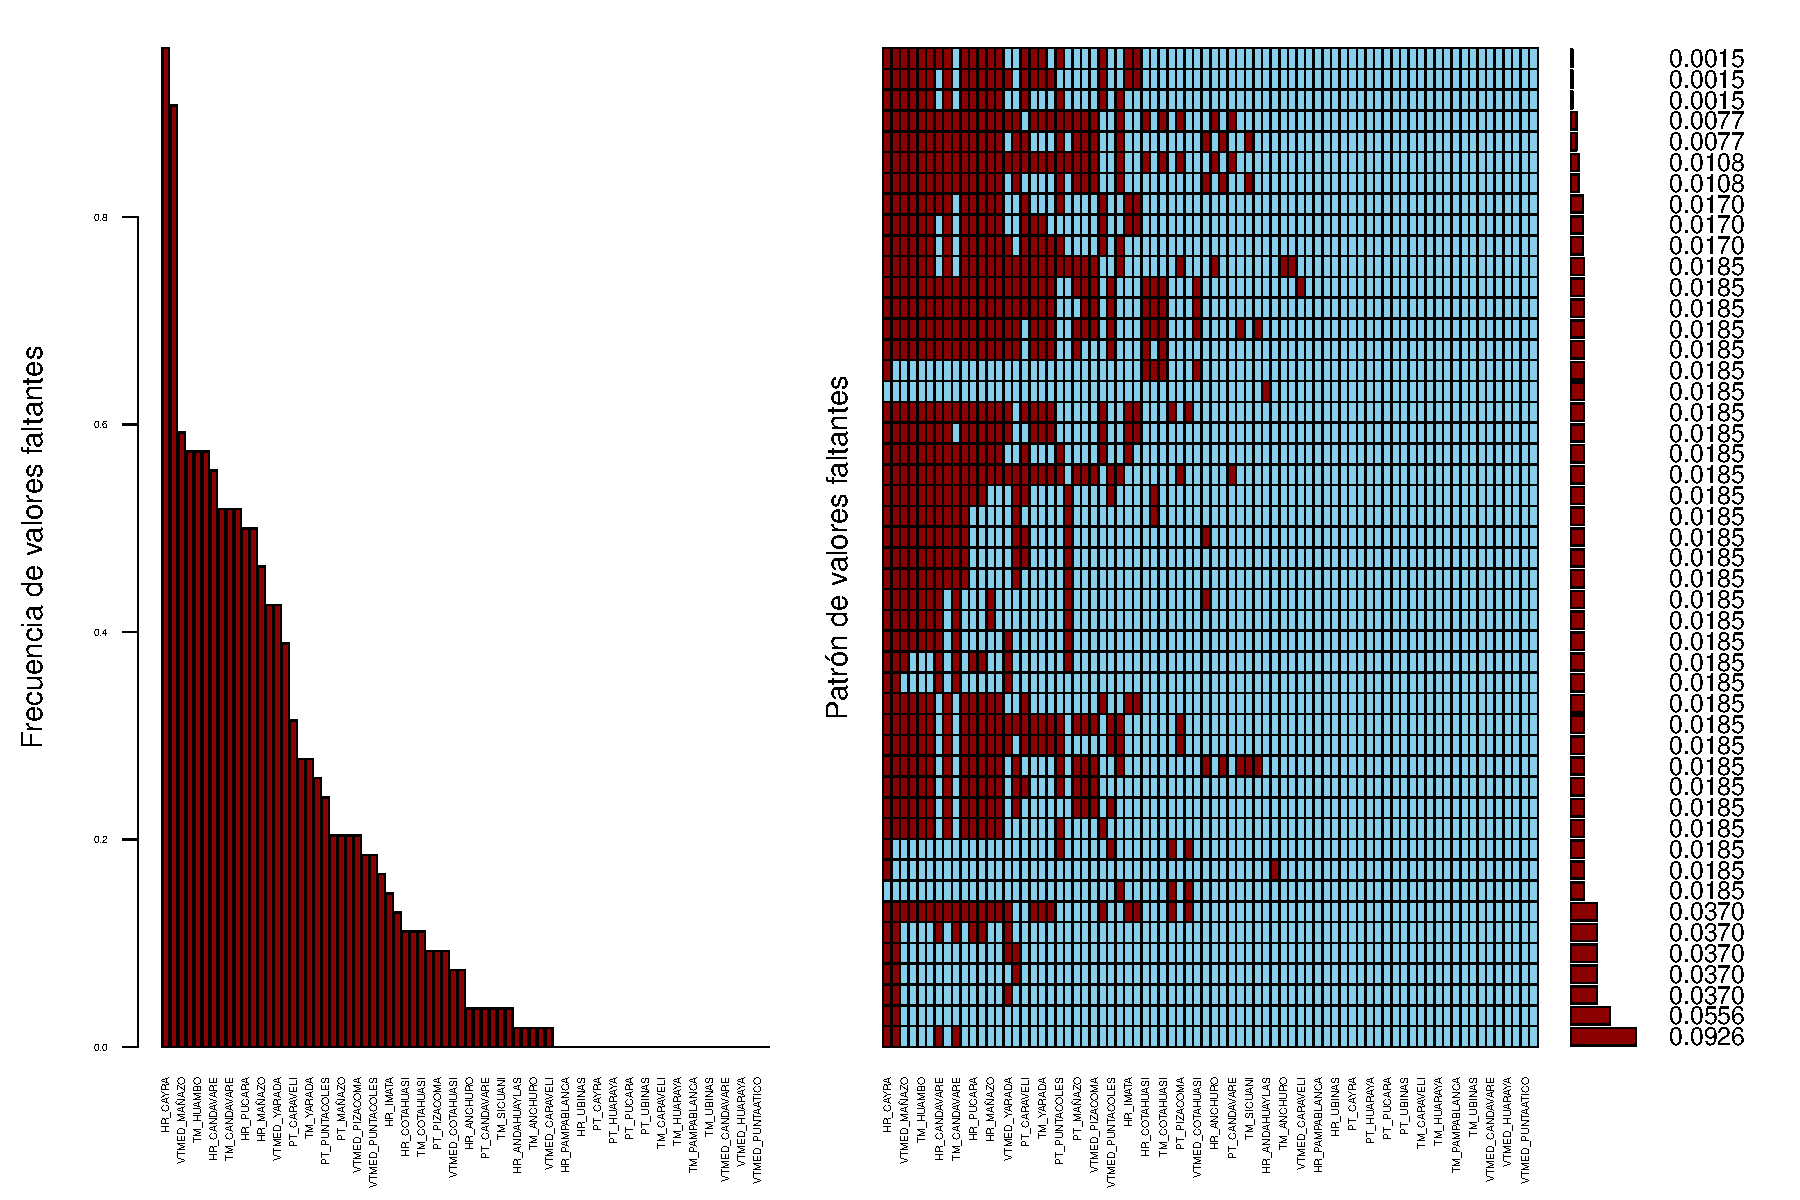
\includegraphics[width=\textwidth]{Capitulos/datos_faltanes/grafico_general.pdf} 
    
    \label{fig:valores_faltantes}
\end{figure}


En la siguiente tabla, se muestran las proporciones de valores faltantes por estación para las variables de **Humedad Relativa (HR)**, **Precipitación (PT)**, **Temperatura (TM)** y **Velocidad Media del Viento (VTMED)**, ordenadas de mayor a menor proporción de valores faltantes.

\begin{table}[H]
    \centering
    \footnotesize  % Reduce aún más el tamaño de la fuente
    \renewcommand{\arraystretch}{1.2}  % Ajusta el espacio entre filas (opcional)
    \setlength{\tabcolsep}{8pt}  % Ajusta el espacio entre las columnas
    \caption{Proporción de Valores Faltantes por Estación y Variable}
    \begin{tabular}{lcccc}
    \hline
    \textbf{Estación} & \textbf{Humedad Rel. (HR)} & \textbf{Precipitación (PT)} & \textbf{Temperatura (TM)} & \textbf{VTMED} \\
    \hline
    CAYRA       & 0.96 & 0.31 & 0.91 & 0.91 \\
    HUAMBO      & 0.57 & 0.26 & 0.59 & 0.57 \\
    CANDAVARE   & 0.56 & 0.24 & 0.57 & 0.37 \\
    CORACORA    & 0.52 & 0.20 & 0.43 & 0.04 \\
    PUCARA      & 0.50 & 0.20 & 0.20 & 0.02 \\
    MAÑAZO      & 0.46 & 0.17 & 0.19 & 0.19 \\
    PIZACOMA    & 0.39 & 0.11 & 0.19 & 0.20 \\
    YARADA      & 0.28 & 0.09 & 0.07 & 0.19 \\
    IMATA       & 0.15 & 0.04 & 0.19 & 0.19 \\
    HUARAYA     & 0.13 & 0.00 & 0.00 & 0.00 \\
    COTAHUASI   & 0.11 & 0.00 & 0.00 & 0.00 \\
    PUNTACOLES  & 0.09 & 0.00 & 0.00 & 0.00 \\
    ANCHURO     & 0.04 & 0.00 & 0.02 & 0.00 \\
    SICUANI     & 0.04 & 0.00 & 0.00 & 0.00 \\
    ANDAHUAYLAS & 0.02 & 0.00 & 0.00 & 0.00 \\
    CARAVELI    & 0.00 & 0.00 & 0.00 & 0.00 \\
    PAMPABLANCA & 0.00 & 0.00 & 0.00 & 0.00 \\
    PUNTAATICO  & 0.00 & 0.00 & 0.00 & 0.00 \\
    UBINAS      & 0.00 & 0.00 & 0.00 & 0.00 \\
    \hline
    \end{tabular}
    \label{tab:datos_faltantes}
\end{table}


\section{Imputación de Datos Faltantes Mediante MICE}

\noindent
En la presente investigación se optó por el uso del algoritmo \textbf{MICE} (\textit{Multiple Imputation by Chained Equations}, que en español se traduce como \textit{Imputación Múltiple mediante Ecuaciones Encadenadas}) para la imputación de los valores faltantes en las estaciones meteorológicas. MICE se basa en la idea de generar \textbf{m} conjuntos de datos completos (cada uno imputado de forma ligeramente diferente), lo que permite capturar la incertidumbre inherente en el proceso de imputación. Cada conjunto imputado es luego analizado de manera independiente, y los resultados se combinan para reflejar dicha variabilidad en las estimaciones finales.

\noindent
La expresión general de MICE puede verse como un procedimiento iterativo, donde cada variable con datos faltantes se modela en función de las demás variables, actualizando sucesivamente las estimaciones en cada paso. Entre cada iteración se utilizan \textit{ecuaciones encadenadas} que llenan los huecos de cada variable tomando en cuenta la información de las restantes. En el presente caso, se empleó el método \textbf{pmm} (\textit{predictive mean matching}), por ser considerado más robusto para datos climáticos; asimismo, se establecieron \texttt{m = 10} imputaciones, \texttt{maxit = 20} iteraciones para lograr convergencia, y se fijó una semilla \texttt{seed = 123} para garantizar la reproducibilidad de los resultados.

\noindent
Se decidió aplicar MICE tras comparar otras técnicas simples de imputación, como la media o la regresión lineal simple, que demostraron un ajuste menos representativo para datos estacionarios propios de las variables hidrometeorológicas. En particular, la imputación mediante ecuaciones encadenadas ofrece la ventaja de respetar la distribución original de los datos y la relación entre variables. Esto reviste especial importancia al modelar fenómenos como la sequía con modelos de dependencia (por ejemplo, cópulas), pues la calidad y completitud de los datos son determinantes para garantizar la validez de las conclusiones.

\section{Análisis de la Tendencia de las Variables Hidrometeorológicas}

El análisis de tendencias es una herramienta crucial para entender cómo evolucionan las variables climáticas a lo largo del tiempo y para predecir sus posibles efectos a largo plazo. En este estudio, se aplicó el análisis de tendencias a varias variables hidrometeorológicas provenientes de diferentes estaciones meteorológicas en el sur del Perú. Las variables consideradas incluyen la humedad relativa (\( X_1 \)), la precipitación (\( X_2 \)), la temperatura (\( X_3 \)) y la velocidad media del viento (\( X_4 \)). El principal objetivo de este análisis es identificar si alguna de estas variables presenta una tendencia significativa con el tiempo, lo que permitiría detectar patrones a largo plazo relevantes para la gestión de recursos hídricos y la planificación agrícola.

Para evaluar la tendencia de las variables hidrometeorológicas, se utilizó la regresión lineal simple, que es una técnica estadística ampliamente utilizada para modelar la relación entre una variable dependiente (\( Y \)) y una variable independiente, que en este caso es el tiempo (\( AÑO \)). La formulación del modelo de regresión lineal es la siguiente:

\[
Y = \beta_0 + \beta_1 \cdot AÑO + \epsilon
\]

Donde:
\begin{itemize}
    \item \( Y \) es la variable dependiente (\( X_1 \), \( X_2 \), \( X_3 \), \( X_4 \)).
    \item \( AÑO \) es la variable independiente que representa el tiempo.
    \item \( \beta_0 \) es el intercepto de la regresión, es decir, el valor de \( Y \) cuando \( AÑO = 0 \).
    \item \( \beta_1 \) es la pendiente de la regresión, que describe la tasa de cambio de la variable dependiente respecto al tiempo.
    \item \( \epsilon \) es el término de error, que refleja la variabilidad no explicada por el modelo.
\end{itemize}

A partir de este modelo, se puede evaluar si la variable de interés presenta una tendencia significativa a lo largo del tiempo.

\subsection{Justificación del Método de Imputación y Elección del Modelo}

Para el análisis de las series temporales, se utilizó el método \texttt{MICE} (Multiple Imputation by Chained Equations), que es particularmente útil para tratar los valores faltantes en datos climáticos. Este enfoque es ideal porque permite capturar la incertidumbre inherente a los valores ausentes y modelar las relaciones complejas entre las variables de las series temporales. Este método fue preferido sobre la imputación por media o la regresión simple, ya que estas técnicas no ofrecieron buenos resultados cuando se probaron en datos con patrones no estacionarios y fluctuaciones no lineales.

El método \texttt{MICE} proporcionó imputaciones más realistas y precisas, ajustándose mejor a la naturaleza de las fluctuaciones observadas en los datos, lo que lo convierte en la opción más adecuada para este estudio.

\subsection{Prueba de Hipótesis}

En el análisis de tendencias, se formula una prueba de hipótesis para determinar si existe una tendencia significativa en los datos. La hipótesis nula (\( H_0 \)) establece que no hay una tendencia significativa en la variable, mientras que la hipótesis alternativa (\( H_1 \)) plantea que sí existe una tendencia significativa. Las hipótesis son:

\[
H_0: \beta_1 = 0 \quad \text{(no hay tendencia significativa)}
\]
\[
H_1: \beta_1 \neq 0 \quad \text{(hay tendencia significativa)}
\]

Se utiliza el valor \( t \) obtenido de la regresión para comparar con el valor crítico \( t \), basado en una distribución \( t \) con un nivel de confianza del 95\%. Si el valor absoluto de \( t \) es mayor que el valor crítico \( t \), se rechaza la hipótesis nula y se concluye que la tendencia es significativa. Si el valor de \( t \) es menor que el valor crítico, no se rechaza la hipótesis nula, lo que indica que no hay suficiente evidencia para afirmar que existe una tendencia significativa.

\subsection{Corrección de la Tendencia}

En caso de que la prueba de hipótesis indique que la tendencia es significativa, el siguiente paso es corregir la serie temporal para eliminar la influencia de dicha tendencia. Para ello, se utiliza el valor de la tendencia ajustada, \( T_{mpt} \), que representa los valores estimados de la variable, ajustados por el modelo de regresión.


Los valores ajustados de la tendencia se obtienen utilizando la función de predicción de la regresión lineal, que se expresa como:

\[
T_{m_{p_t}} = \hat{Y} = \beta_0 + \beta_1 \cdot AÑO
\]


Donde \( \hat{Y} \) es la serie temporal ajustada que refleja la tendencia. En este caso, \( T_{\text{mpt}} \) es el valor de la tendencia calculado para cada observación en el tiempo \( AÑO \). Si la serie temporal original tiene una tendencia significativa, esta se elimina restando los valores de \( T_{\text{mpt}} \) de la serie original y ajustando los valores para reflejar solo la variabilidad intrínseca de los datos.


Una vez calculados los valores ajustados, se procede a sustituir los valores negativos (si los hubiera) por cero, dado que no tiene sentido tener valores negativos para estas variables climáticas.

Los coeficientes \( A_m \) y \( B_m \) son los valores estimados del intercepto y la pendiente de la regresión lineal, respectivamente, y se usan para ajustar los datos de acuerdo con la fórmula:

\[
Y_{\text{ajustada}} = Y - T_{\text{mpt}} + \text{media}(Y)
\]


De este modo, se genera una serie temporal "sin tendencia", en la que se eliminan los efectos de la tendencia temporal, dejando solo la variabilidad natural de los datos.

\subsection{Resumen del Procedimiento}

En resumen, el análisis de tendencias mediante regresión lineal y el uso del método \texttt{MICE} permitió realizar un análisis robusto de las variables climáticas. La identificación de tendencias significativas en varias de las estaciones meteorológicas permitió proceder con la corrección de estas tendencias, asegurando que las series temporales utilizadas en el análisis posterior reflejan únicamente la variabilidad intrínseca de los datos sin ser sesgadas por tendencias temporales que podrían alterar los resultados.

El procedimiento realizado garantiza que las series temporales analizadas son fiables y adecuadas para la realización de estudios futuros sobre las variables hidrometeorológicas.

\begin{landscape}
\begin{table}[ht]
\centering
\caption{Resumen de estaciones meteorológicas: coeficientes de determinación ($r^2$) y estadísticas $t$ para las variables HR, PT, TM y VTMED}
\begin{adjustbox}{valign=c, width=\textwidth}
\begin{tabular}{lcccccccc}
\toprule
\textbf{Estación} & \textbf{HR $r^2$} & \textbf{HR t} & \textbf{PT $r^2$} & \textbf{PT t} & \textbf{TM $r^2$} & \textbf{TM t} & \textbf{VTMED $r^2$} & \textbf{VTMED t} \\
\midrule
ANCACHURO     & 0.160 & 11.103 & 0.001 &  0.836 & 0.021 &  3.685 & 0.026 &  4.123 \\
COTAHUASI     & 0.150 & 10.662 & 0.000 & -0.206 & 0.150 & 10.662 & 0.037 & -4.993 \\
ANDAHUAYLAS   & 0.312 & 17.106 & 0.004 &  1.705 & 0.022 &  3.797 & 0.314 & -17.188 \\
CANDAVARE     & 0.012 & -2.796 & 0.001 &  0.695 & 0.000 &  0.476 & 0.020 & -3.658 \\
CARAVELI      & 0.000 & -2.961 & 0.061 &  6.465 & 0.108 &  8.823 & 0.061 &  6.465 \\
CORACORA      & 0.006 & -1.971 & 0.001 &  0.827 & 0.030 &  4.506 & 0.179 & -11.865 \\
CAYRA         & 0.025 &  4.102 & 0.000 &  0.152 & 0.025 &  4.102 & 0.203 & 12.808 \\
HUAMBO        & 0.011 & -2.661 & 0.000 &  0.520 & 0.000 &  0.602 & 0.136 & -10.103 \\
HUARAYA       & 0.000 & -0.225 & 0.000 & -1.488 & 0.000 &  1.649 & 0.263 & -15.200 \\
IMATA         & 0.016 &  3.220 & 0.000 & -0.357 & 0.034 &  4.747 & 0.016 &  3.237 \\
YARADA        & 0.087 &  7.837 & 0.000 &  0.287 & 0.000 &  1.649 & 0.022 & -3.812 \\
MANAZO        & 0.057 &  6.276 & 0.000 & -1.344 & 0.026 &  4.154 & 0.007 &  2.060 \\
PAMPABLANCA   & 0.061 & -6.493 & 0.021 & -3.702 & 0.012 &  2.846 & 0.371 & -19.529 \\
PIZACOMA      & 0.075 & -7.260 & 0.004 & -1.550 & 0.015 &  3.170 & 0.092 & -8.101 \\
PUCARA        & 0.161 & -11.138& 0.000 & -1.190 & 0.000 &  0.831 & 0.058 &  1.475 \\
PUNTAATICO    & 0.090 &  8.010 & 0.000 & -0.879 & 0.000 &  1.112 & 0.008 &  2.264 \\
PUNTACOLES    & 0.018 &  3.485 & 0.009 &  2.437 & 0.006 &  2.001 & 0.035 & -4.839 \\
SICUANI       & 0.029 &  4.404 & 0.000 &  0.393 & 0.000 & -1.205 & 0.309 & -16.990 \\
UBINAS        & 0.000 &  0.057 & 0.000 &  0.615 & 0.000 &  2.441 & 0.147 & -10.571 \\
\bottomrule
\end{tabular}
\end{adjustbox}
\end{table}
\vspace{0.2cm}  % Espacio entre la tabla y la nota
\begin{justify}
\small \textbf{\textit{Nota.}} HR = Humedad Relativa, PT = Precipitación Total, TM = Temperatura Media, VTMED = Velocidad del Viento Media. Los valores de $r^2$ indican el coeficiente de determinación y los valores t provienen del test de significancia. Análisis realizado en R.
\end{justify}

\end{landscape}



En la tabla presentada, se resumen las estaciones meteorológicas analizadas, junto con las variables correspondientes y los resultados obtenidos del análisis de tendencias. Se incluyen dos parámetros principales: el coeficiente de determinación \(r^2\) y el valor de \(t\) calculado para cada variable en cada estación.

\paragraph{Coeficiente de Determinación \(r^2\):} El coeficiente de determinación \(r^2\) refleja la proporción de la variabilidad de la variable dependiente (como la humedad relativa, la precipitación, la temperatura o la velocidad del viento) que puede ser explicada por la variable independiente (el tiempo). Cuanto mayor sea el valor de \(r^2\), mayor es la capacidad del modelo para explicar la variabilidad de la variable con respecto al tiempo. Un \(r^2\) cercano a 1 sugiere una fuerte relación entre la variable y el tiempo, mientras que valores cercanos a 0 indican que el tiempo tiene poca o ninguna influencia en la variable.

\paragraph{Valor de t Calculado:} El valor de \(t\) calculado se utiliza para evaluar la significancia estadística de la tendencia. Un valor absoluto de \(t\) mayor que el valor crítico (\(t_{crítico} = 1.964\) con un nivel de confianza del 95\%) indica que la tendencia es significativa. Esto implica que la variable presenta una relación estadísticamente significativa con el tiempo. Si el valor de \(t\) es menor que el valor crítico, no se puede concluir que exista una tendencia significativa.

\paragraph{Estaciones con Tendencias Significativas:} En las estaciones que muestran tendencias significativas, los valores de \(r^2\) y \(t\) indican que el tiempo tiene una influencia considerable en las variables analizadas. Por ejemplo, en la estación ANDAHUAYLAS la variable Humedad relativa, el coeficiente de determinación es \(r^2 = 0.312\), lo que indica una moderada capacidad de explicación del modelo. Además, el valor de \(t = 17.106\) es mucho mayor que el valor crítico de 1.964, lo que confirma que la tendencia es significativa. De manera similar, en estaciones como **TM\_COTAHUASI** y **VTMED\_YARADA**, los valores de \(t\) también superan el valor crítico, lo que sugiere que las variables presentan tendencias significativas con el tiempo.

\paragraph{Estaciones con Tendencias No Significativas:} En contraste, algunas estaciones presentan tendencias no significativas. Por ejemplo, en la estación **PT\_ANCACHURO**, el coeficiente de determinación es \(r^2 = 0.001\) y el valor de \(t = 0.836\) es inferior al valor crítico de 1.964, lo que indica que no hay suficiente evidencia para concluir que existe una tendencia significativa en la precipitación de esta estación. Otras estaciones como **PT\_COTAHUASI** y **PT\_PUNTAATICO** también presentan valores de \(r^2\) cercanos a 0 y valores de \(t\) menores que el valor crítico, lo que significa que las tendencias no son estadísticamente significativas.

\paragraph{Implicaciones de los Resultados:} Las estaciones que presentan tendencias significativas en variables clave, como la **humedad relativa** y la **temperatura media**, pueden ser cruciales para la toma de decisiones en sectores como la agricultura y la gestión de recursos hídricos. Por ejemplo, las estaciones **ANDAHUAYLAS** y **CANDAVARE** muestran tendencias significativas en la humedad relativa, lo que puede influir en la planificación de cultivos y la gestión del agua. Por otro lado, las estaciones sin tendencias significativas, como **PT\_ANCACHURO**, sugieren que la precipitación no está siendo afectada por una tendencia temporal clara en los últimos años.

En conclusión, este análisis proporciona una comprensión detallada de cómo las variables hidrometeorológicas están cambiando con el tiempo en diferentes estaciones, lo que puede ser útil para los estudios de cambio climático y la planificación de estrategias de adaptación a largo plazo.


\begin{table}[ht!]
\centering
\caption{Análisis de correlaciones climáticas por estación}
\resizebox{\textwidth}{!}{%
\begin{tabular}{lcccccl}
\toprule
\textbf{Estación} & \textbf{PT-HR} & \textbf{PT-TM} & \textbf{HR-TM} & \textbf{VTMED} & \textbf{Multicolinealidad} & \textbf{Sugerencia de Variables} \\
\midrule
Andahuaylas        & Moderada        & Moderada        & Baja            & Baja             & No                  & PT, HR, TM                   \\
Ancachuro          & Moderada        & Fuerte          & Moderada        & Baja             & Posible             & Evitar usar PT y TM juntas \\
Cayra              & Baja            & Moderada        & Muy baja        & Baja             & No                  & Priorizar TM                 \\
Sicuani            & Fuerte          & Moderada        & Baja            & Baja             & Posible             & HR clave, cuidado con PT     \\
Pucara             & Moderada        & Moderada        & Baja            & Baja             & No                  & PT, TM, HR                   \\
Manazo             & Fuerte          & Baja            & Muy baja        & Baja             & Posible             & HR clave, PT opcional        \\
Huaraya            & Moderada        & Moderada        & Baja            & Baja             & No                  & PT, HR, TM                   \\
Coracora           & Moderada        & Baja            & Moderada        & Baja             & No                  & Priorizar HR                 \\
Cotahuasi          & Fuerte          & Baja            & Baja            & Baja             & Posible             & Priorizar HR                 \\
Caravelí           & Baja            & Baja            & Baja            & Baja             & No                  & Variables independientes     \\
Huambo             & Fuerte          & Moderada        & Moderada        & Moderada         & Sí                  & Elegir una entre PT/HR y TM/VTMED \\
Candavare          & Moderada        & Moderada        & Muy fuerte      & Baja             & Alta                & Evitar usar HR y TM juntas   \\
Imata              & Fuerte          & Moderada        & Baja            & Baja             & Posible             & Priorizar HR y TM            \\
Ubinas             & Fuerte          & Baja            & Baja            & Moderada negativa & Posible             & Priorizar HR                 \\
Pizacoma           & Moderada        & Moderada        & Baja            & Baja             & No                  & HR relevante                 \\
Yarada             & Muy baja        & Baja            & Moderada negativa & Baja             & No                  & Variables independientes     \\
Pampablanca        & Baja            & Baja            & Moderada negativa & Baja             & No                  & Evaluar HR y TM (negativa)   \\
Puntaatico         & Baja            & Baja            & Moderada negativa & Baja             & No                  & Variables independientes     \\
Puntacoles         & Baja            & Baja            & Baja            & Baja             & No                  & Variables independientes     \\
\bottomrule
\end{tabular}%
}
\end{table}







  % Inicia la orientación horizontal

\begin{table}[ht]
\centering
\small
\caption{Resultados de correlaciones SPI vs variables climáticas por estación}
\resizebox{\textwidth}{!}{%
\begin{tabular}{ccccc}
\hline
\rowcolor{gray!20} \textbf{Estación} & \textbf{Pearson} & \textbf{Spearman} & \textbf{Kendall} & \textbf{Covarianza} \\
\hline
\rowcolor{gray!10} ANDAHUAYLAS & 0.33 & 0.34 & 0.23 & 2.44 \\
\rowcolor{white} ANCACHURO   & 0.46 & 0.47 & 0.32 & 4.09 \\
\rowcolor{gray!10} CAYRA       & 0.16 & 0.18 & 0.12 & 0.88 \\
\rowcolor{white} SICUANI     & 0.71 & 0.75 & 0.55 & 7.63 \\
\rowcolor{gray!10} PUCARA      & 0.41 & 0.41 & 0.28 & 4.82 \\
\rowcolor{white} MANAZO      & 0.68 & 0.70 & 0.51 & 9.43 \\
\rowcolor{gray!10} HUARAYA     & 0.44 & 0.47 & 0.33 & 4.30 \\
\rowcolor{white} CORACORA    & 0.58 & 0.61 & 0.43 & 10.29 \\
\rowcolor{gray!10} COTAHUASI   & 0.75 & 0.77 & 0.57 & 14.56 \\
\rowcolor{white} CARAVELI    & 0.35 & 0.42 & 0.28 & 5.79 \\
\rowcolor{gray!10} HUAMBO      & 0.69 & 0.71 & 0.51 & 12.51 \\
\rowcolor{white} CANDAVARE   & 0.53 & 0.60 & 0.42 & 9.19 \\
\hline
\end{tabular}%
}
\end{table}







\section{Analisis de la curva doble masa}


\begin{landscape}
\begin{table}[htbp]
\centering
\caption{Matriz de correlación de Humedad Relativa entre estaciones}
\arrayrulecolor[HTML]{006400}
\resizebox{1.4\textwidth}{!}{%
\begin{tabular}{lccccccccccccccccccc}
\toprule
\rowcolor{gray!20} % Color para las celdas del encabezado
 & ANC & COT & AND & CAN & CAR & COR & CAY & HUA & HRY & IMA & YAR & MAN & PBL & PIZ & PUC & PTA & PTC & SIC & UBI \\
\midrule
\arrayrulecolor[HTML]{006400} % Color de las líneas (verde oscuro)
\textbf{ANC}  & 1.00  & 0.46  & 0.49  & 0.35  & 0.44  & 0.24  & 0.03  & 0.26  & 0.26  & 0.36  & 0.07  & 0.41  & -0.43 & 0.14  & -0.13 & -0.19 & -0.16 & 0.33  & 0.33  \\
\textbf{COT}  & 0.46  & 1.00  & 0.33  & 0.66  & 0.63  & 0.75  & 0.19  & 0.86  & 0.43  & 0.71  & -0.30 & 0.76  & -0.32 & 0.51  & 0.38  & -0.31 & -0.04 & 0.69  & 0.82  \\
\textbf{AND}  & 0.49  & 0.33  & 1.00  & 0.18  & 0.34  & 0.17  & 0.12  & 0.19  & 0.19  & 0.35  & 0.06  & 0.38  & -0.33 & 0.20  & -0.26 & -0.05 & -0.08 & 0.38  & 0.26  \\
\textbf{CAN}  & 0.35  & 0.66  & 0.18  & 1.00  & 0.49  & 0.56  & 0.12  & 0.55  & 0.41  & 0.48  & -0.25 & 0.44  & -0.21 & 0.40  & 0.27  & -0.35 & -0.06 & 0.45  & 0.56  \\
\textbf{CAR}  & 0.44  & 0.63  & 0.34  & 0.49  & 1.00  & 0.41  & 0.11  & 0.56  & 0.40  & 0.49  & -0.14 & 0.52  & -0.29 & 0.42  & 0.12  & -0.33 & 0.01  & 0.41  & 0.57  \\
\textbf{COR}  & 0.24  & 0.75  & 0.17  & 0.56  & 0.41  & 1.00  & 0.04  & 0.69  & 0.24  & 0.57  & -0.30 & 0.52  & -0.30 & 0.41  & 0.39  & -0.30 & -0.10 & 0.60  & 0.69  \\
\textbf{CAY}  & 0.03  & 0.19  & 0.12  & 0.12  & 0.11  & 0.04  & 1.00  & 0.17  & -0.01 & 0.22  & -0.38 & 0.33  & 0.04  & 0.13  & 0.12  & -0.06 & 0.19  & 0.18  & 0.15  \\
\textbf{HUA}  & 0.26  & 0.86  & 0.19  & 0.55  & 0.56  & 0.69  & 0.17  & 1.00  & 0.45  & 0.65  & -0.32 & 0.74  & -0.24 & 0.57  & 0.46  & -0.29 & -0.05 & 0.69  & 0.81  \\
\textbf{HRY}  & 0.26  & 0.43  & 0.19  & 0.41  & 0.40  & 0.24  & -0.01 & 0.45  & 1.00  & 0.22  & 0.00  & 0.30  & -0.35 & 0.45  & 0.08  & -0.07 & -0.03 & 0.38  & 0.44  \\
\textbf{IMA}  & 0.36  & 0.71  & 0.35  & 0.48  & 0.49  & 0.57  & 0.22  & 0.65  & 0.22  & 1.00  & -0.20 & 0.70  & -0.12 & 0.49  & 0.34  & -0.21 & 0.06  & 0.60  & 0.69  \\
\textbf{YAR}  & 0.07  & -0.30 & 0.06  & -0.25 & -0.14 & -0.30 & -0.38 & -0.32 & 0.00  & -0.20 & 1.00  & -0.16 & -0.06 & -0.25 & -0.41 & 0.21  & -0.07 & -0.13 & -0.28 \\
\textbf{MAN}  & 0.41  & 0.76  & 0.38  & 0.44  & 0.52  & 0.52  & 0.33  & 0.74  & 0.30  & 0.70  & -0.16 & 1.00  & -0.21 & 0.39  & 0.32  & -0.17 & 0.03  & 0.74  & 0.70  \\
\textbf{PBL}  & -0.43 & -0.32 & -0.33 & -0.21 & -0.29 & -0.30 & 0.04  & -0.24 & -0.35 & -0.12 & -0.06 & -0.21 & 1.00  & -0.11 & -0.11 & 0.21  & 0.10  & -0.28 & -0.34 \\
\textbf{PIZ}  & 0.14  & 0.51  & 0.20  & 0.40  & 0.42  & 0.41  & 0.13  & 0.57  & 0.45  & 0.49  & -0.25 & 0.39  & -0.11 & 1.00  & 0.27  & -0.23 & -0.13 & 0.36  & 0.56  \\
\textbf{PUC}  & -0.13 & 0.38  & -0.26 & 0.27  & 0.12  & 0.39  & 0.12  & 0.46  & 0.08  & 0.34  & -0.41 & 0.32  & 0.11  & 0.27  & 1.00  & -0.23 & -0.06 & 0.10  & 0.39  \\
\textbf{PTA}  & -0.19 & -0.31 & -0.05 & -0.35 & -0.33 & -0.30 & -0.06 & -0.29 & -0.07 & -0.21 & 0.21  & -0.17 & 0.21  & -0.23 & -0.23 & 1.00  & 0.16  & -0.21 & -0.34 \\
\textbf{PTC}  & -0.16 & -0.04 & -0.08 & -0.06 & 0.01  & -0.10 & 0.19  & -0.05 & -0.03 & 0.06  & -0.07 & 0.03  & 0.10  & -0.13 & 0.10  & 1.00  & -0.08 & -0.02 & -0.02 \\
\textbf{SIC}  & 0.33  & 0.69  & 0.38  & 0.45  & 0.41  & 0.60  & 0.18  & 0.69  & 0.38  & 0.60  & -0.13 & 0.74  & -0.28 & 0.36  & 0.23  & -0.21 & -0.08 & 1.00  & 0.70  \\
\textbf{UBI}  & 0.33  & 0.82  & 0.26  & 0.56  & 0.57  & 0.69  & 0.15  & 0.81  & 0.44  & 0.69  & -0.28 & 0.70  & -0.34 & 0.56  & 0.39  & -0.34 & -0.02 & 0.70  & 1.00  \\
\hline
\end{tabular}
}
\vspace{0.5em}
\begin{flushleft}
\footnotesize
\textbf{\textit{Nota}}: ANC = Ancachuro, COT = Cotahuasi, AND = Andahuaylas, CAN = Candavare, CAR = Caravelí, COR = Coracora, CAY = Cayra, HUA = Huambo, HRY = Huaraya, IMA = Imata, YAR = Yarada, MAN = Mañazo, PBL = Pampablanca, PIZ = Pizacoma, PUC = Pucará, PTA = Punta Atico, PTC = Punta Coles, SIC = Sicuani, UBI = Ubinas.
\end{flushleft}
\end{table}
\end{landscape}



\begin{landscape}
\begin{table}[htbp]
\centering
\caption{Matriz de correlación de temperatura media entre estaciones}
\arrayrulecolor[HTML]{006400}
\resizebox{1.4\textwidth}{!}{%
\begin{tabular}{lccccccccccccccccccc}
\toprule
\rowcolor{gray!20} % Color para las celdas del encabezado
 & ANC & COT & AND & CAN & CAR & COR & CAY & HUA & HRY & IMA & YAR & MAN & PBL & PIZ & PUC & PTA & PTC & SIC & UBI \\
\midrule
\arrayrulecolor[HTML]{006400} % Color de las líneas (verde oscuro)
\textbf{ANC}  & 1.00  & 0.51  & 0.83  & 0.63  & 0.70  & 0.69  & 0.83  & 0.69  & 0.83  & 0.88  & 0.63  & 0.75  & 0.69  & 0.84  & 0.81  & 0.60  & 0.64  & 0.79  & 0.81  \\
\textbf{COT}  & 0.51  & 1.00  & 0.68  & 0.56  & 0.74  & 0.69  & 0.65  & 0.58  & 0.62  & 0.55  & 0.22  & 0.69  & 0.24  & 0.60  & 0.54  & 0.19  & 0.26  & 0.56  & 0.66  \\
\textbf{AND}  & 0.83  & 0.68  & 1.00  & 0.76  & 0.76  & 0.79  & 0.90  & 0.69  & 0.88  & 0.86  & 0.55  & 0.85  & 0.60  & 0.88  & 0.85  & 0.52  & 0.57  & 0.85  & 0.87  \\
\textbf{CAN}  & 0.63  & 0.56  & 0.76  & 1.00  & 0.62  & 0.76  & 0.69  & 0.59  & 0.73  & 0.69  & 0.41  & 0.65  & 0.43  & 0.75  & 0.66  & 0.37  & 0.44  & 0.70  & 0.72  \\
\textbf{CAR}  & 0.70  & 0.74  & 0.76  & 0.62  & 1.00  & 0.74  & 0.78  & 0.73  & 0.74  & 0.76  & 0.48  & 0.70  & 0.54  & 0.75  & 0.70  & 0.47  & 0.52  & 0.67  & 0.77  \\
\textbf{COR}  & 0.69  & 0.69  & 0.79  & 0.76  & 0.74  & 1.00  & 0.76  & 0.67  & 0.73  & 0.74  & 0.39  & 0.70  & 0.41  & 0.75  & 0.69  & 0.32  & 0.40  & 0.75  & 0.81  \\
\textbf{CAY}  & 0.83  & 0.65  & 0.90  & 0.69  & 0.78  & 0.76  & 1.00  & 0.72  & 0.89  & 0.86  & 0.50  & 0.85  & 0.56  & 0.87  & 0.85  & 0.47  & 0.53  & 0.86  & 0.87  \\
\textbf{HUA}  & 0.69  & 0.58  & 0.69  & 0.59  & 0.73  & 0.67  & 0.72  & 1.00  & 0.71  & 0.76  & 0.50  & 0.63  & 0.56  & 0.68  & 0.73  & 0.51  & 0.54  & 0.69  & 0.76  \\
\textbf{HRY}  & 0.83  & 0.62  & 0.88  & 0.73  & 0.74  & 0.73  & 0.89  & 0.71  & 1.00  & 0.86  & 0.57  & 0.87  & 0.61  & 0.89  & 0.88  & 0.59  & 0.54  & 0.88  & 0.84  \\
\textbf{IMA}  & 0.88  & 0.55  & 0.86  & 0.69  & 0.76  & 0.74  & 0.86  & 0.76  & 0.86  & 1.00  & 0.72  & 0.78  & 0.77  & 0.90  & 0.87  & 0.69  & 0.73  & 0.79  & 0.88  \\
\textbf{YAR}  & 0.63  & 0.22  & 0.55  & 0.41  & 0.48  & 0.39  & 0.50  & 0.50  & 0.57  & 0.72  & 1.00  & 0.37  & 0.95  & 0.64  & 0.63  & 0.94  & 0.94  & 0.44  & 0.54  \\
\textbf{MAN}  & 0.75  & 0.69  & 0.85  & 0.65  & 0.70  & 0.70  & 0.85  & 0.63  & 0.87  & 0.78  & 0.37  & 1.00  & 0.44  & 0.83  & 0.82  & 0.36  & 0.42  & 0.78  & 0.81  \\
\textbf{PBL}  & 0.69  & 0.24  & 0.60  & 0.43  & 0.54  & 0.41  & 0.56  & 0.56  & 0.61  & 0.77  & 0.95  & 0.44  & 1.00  & 0.69  & 0.67  & 0.97  & 0.97  & 0.47  & 0.58  \\
\textbf{PIZ}  & 0.84  & 0.60  & 0.88  & 0.75  & 0.75  & 0.75  & 0.87  & 0.68  & 0.89  & 0.90  & 0.64  & 0.83  & 0.69  & 1.00  & 0.87  & 0.60  & 0.66  & 0.81  & 0.88  \\
\textbf{PUC}  & 0.81  & 0.54  & 0.86  & 0.66  & 0.70  & 0.69  & 0.85  & 0.73  & 0.88  & 0.87  & 0.63  & 0.82  & 0.67  & 0.87  & 1.00  & 0.61  & 0.63  & 0.83  & 0.84  \\
\textbf{PTA}  & 0.60  & 0.19  & 0.52  & 0.37  & 0.47  & 0.32  & 0.47  & 0.51  & 0.54  & 0.69  & 0.94  & 0.42  & 0.97  & 0.60  & 0.61  & 1.00  & 0.96  & 0.39  & 0.50  \\
\textbf{PTC}  & 0.64  & 0.26  & 0.57  & 0.44  & 0.52  & 0.40  & 0.53  & 0.54  & 0.59  & 0.73  & 0.94  & 0.42  & 0.97  & 0.66  & 0.63  & 0.96  & 1.00  & 0.44  & 0.56  \\
\textbf{SIC}  & 0.79  & 0.56  & 0.85  & 0.70  & 0.67  & 0.75  & 0.86  & 0.69  & 0.88  & 0.79  & 0.44  & 0.78  & 0.47  & 0.81  & 0.83  & 0.44  & 0.39  & 1.00  & 0.81  \\
\textbf{UBI}  & 0.81  & 0.66  & 0.87  & 0.72  & 0.77  & 0.81  & 0.87  & 0.76  & 0.84  & 0.88  & 0.54  & 0.81  & 0.58  & 0.88  & 0.84  & 0.50  & 0.56  & 0.81  & 1.00  \\
\hline
\end{tabular}
}
\vspace{0.5em}
\begin{flushleft}
\footnotesize
\textbf{\textit{Nota}}: ANC = Ancachuro, COT = Cotahuasi, AND = Andahuaylas, CAN = Candavare, CAR = Caravelí, COR = Coracora, CAY = Cayra, HUA = Huambo, HRY = Huaraya, IMA = Imata, YAR = Yarada, MAN = Mañazo, PBL = Pampablanca, PIZ = Pizacoma, PUC = Pucará, PTA = Punta Atico, PTC = Punta Coles, SIC = Sicuani, UBI = Ubinas.
\end{flushleft}
\end{table}
\end{landscape}


\begin{landscape}
\begin{table}[htbp]
\centering
\caption{Matriz de correlación de precipitación entre estaciones}
\arrayrulecolor[HTML]{006400}
\resizebox{1.4\textwidth}{!}{%
\begin{tabular}{lccccccccccccccccccc}
\toprule
\rowcolor{gray!20} % Color para las celdas del encabezado
 & ANC & COT & AND & CAN & CAR & COR & CAY & HUA & HRY & IMA & YAR & MAN & PBL & PIZ & PUC & PTA & PTC & SIC & UBI \\
\midrule
\arrayrulecolor[HTML]{006400} % Color de las líneas (verde oscuro)
\textbf{ANC}  & 1.00  & 0.62  & 0.78  & 0.59  & 0.30  & 0.60  & 0.91  & 0.63  & 0.78  & 0.76  & -0.10 & 0.77  & 0.08  & 0.73  & 0.81  & 0.14  & -0.10 & 0.87  & 0.65  \\
\textbf{COT}  & 0.62  & 1.00  & 0.71  & 0.77  & 0.47  & 0.83  & 0.62  & 0.88  & 0.63  & 0.81  & -0.03 & 0.74  & 0.11  & 0.68  & 0.64  & 0.09  & -0.05 & 0.69  & 0.85  \\
\textbf{AND}  & 0.78  & 0.71  & 1.00  & 0.67  & 0.40  & 0.72  & 0.78  & 0.73  & 0.70  & 0.79  & -0.05 & 0.79  & 0.09  & 0.69  & 0.75  & 0.13  & -0.07 & 0.83  & 0.74  \\
\textbf{CAN}  & 0.59  & 0.77  & 0.67  & 1.00  & 0.55  & 0.79  & 0.61  & 0.81  & 0.61  & 0.80  & 0.06  & 0.70  & 0.16  & 0.70  & 0.61  & 0.10  & 0.01  & 0.63  & 0.87  \\
\textbf{CAR}  & 0.30  & 0.47  & 0.40  & 0.55  & 1.00  & 0.53  & 0.32  & 0.52  & 0.29  & 0.42  & 0.09  & 0.33  & 0.07  & 0.30  & 0.30  & 0.02  & 0.03  & 0.34  & 0.49  \\
\textbf{COR}  & 0.60  & 0.83  & 0.72  & 0.79  & 0.53  & 1.00  & 0.62  & 0.83  & 0.58  & 0.80  & -0.02 & 0.69  & 0.07  & 0.66  & 0.61  & 0.11  & -0.06 & 0.67  & 0.83  \\
\textbf{CAY}  & 0.91  & 0.62  & 0.78  & 0.61  & 0.32  & 0.62  & 1.00  & 0.62  & 0.81  & 0.78  & -0.12 & 0.81  & 0.05  & 0.78  & 0.85  & 0.15  & -0.10 & 0.88  & 0.68  \\
\textbf{HUA}  & 0.63  & 0.88  & 0.73  & 0.81  & 0.52  & 0.83  & 0.62  & 1.00  & 0.63  & 0.84  & 0.00  & 0.75  & 0.10  & 0.72  & 0.73  & 0.11  & -0.04 & 0.66  & 0.89  \\
\textbf{HRY}  & 0.78  & 0.63  & 0.70  & 0.61  & 0.29  & 0.58  & 0.81  & 0.63  & 1.00  & 0.80  & -0.07 & 0.84  & 0.09  & 0.83  & 0.88  & 0.10  & -0.08 & 0.81  & 0.71  \\
\textbf{IMA}  & 0.76  & 0.81  & 0.79  & 0.80  & 0.42  & 0.80  & 0.78  & 0.84  & 0.80  & 1.00  & -0.02 & 0.86  & 0.12  & 0.85  & 0.79  & 0.15  & -0.06 & 0.79  & 0.89  \\
\textbf{YAR}  & -0.10 & -0.03 & -0.05 & 0.06  & 0.09  & -0.02 & -0.12 & 0.00  & -0.07 & -0.02 & 1.00  & -0.08 & 0.28  & -0.03 & -0.08 & 0.02  & 0.13  & 0.13  & 0.03  \\
\textbf{MAN}  & 0.77  & 0.74  & 0.79  & 0.70  & 0.33  & 0.69  & 0.81  & 0.75  & 0.84  & 0.86  & -0.08 & 1.00  & 0.10  & 0.87  & 0.85  & 0.18  & -0.06 & 0.84  & 0.78  \\
\textbf{PBL}  & 0.08  & 0.11  & 0.09  & 0.16  & 0.07  & 0.07  & 0.05  & 0.10  & 0.09  & 0.12  & 0.28  & 0.10  & 1.00  & 0.10  & 0.06  & 0.23  & 0.18  & 0.07  & 0.13  \\
\textbf{PIZ}  & 0.73  & 0.68  & 0.69  & 0.70  & 0.75  & 0.75  & 0.87  & 0.72  & 0.83  & 0.90  & 0.64  & 0.83  & 0.69  & 1.00  & 0.79  & 0.18  & -0.06 & 0.76  & 0.78  \\
\textbf{PUC}  & 0.81  & 0.64  & 0.75  & 0.61  & 0.70  & 0.69  & 0.85  & 0.73  & 0.88  & 0.87  & 0.63  & 0.82  & 0.67  & 0.87  & 1.00  & 0.15  & -0.06 & 0.79  & 0.69  \\
\textbf{PTA}  & 0.14  & 0.09  & 0.13  & 0.10  & 0.02  & 0.11  & 0.15  & 0.11  & 0.10  & 0.15  & 0.02  & 0.18  & 0.06  & 0.18  & 0.15  & 1.00  & 0.32  & 0.16  & 0.10  \\
\textbf{PTC}  & -0.10 & -0.05 & -0.07 & 0.01  & 0.03  & -0.06 & -0.10 & -0.04 & -0.08 & -0.06 & 0.13  & -0.06 & 0.18  & -0.06 & -0.06 & 0.32  & 1.00  & -0.09 & -0.03  \\
\textbf{SIC}  & 0.87  & 0.69  & 0.83  & 0.63  & 0.34  & 0.67  & 0.88  & 0.66  & 0.81  & 0.79  & 0.44  & 0.78  & 0.47  & 0.76  & 0.79  & 0.07  & -0.09 & 1.00  & 0.70  \\
\textbf{UBI}  & 0.65  & 0.85  & 0.74  & 0.87  & 0.49  & 0.83  & 0.68  & 0.89  & 0.71  & 0.88  & 0.03  & 0.78  & 0.13  & 0.78  & 0.69  & 0.10  & -0.03 & 0.70  & 1.00  \\
\hline
\end{tabular}
}
\vspace{0.5em}
\begin{flushleft}
\footnotesize
\textbf{\textit{Nota}}: ANC = Ancachuro, COT = Cotahuasi, AND = Andahuaylas, CAN = Candavare, CAR = Caravelí, COR = Coracora, CAY = Cayra, HUA = Huambo, HRY = Huaraya, IMA = Imata, YAR = Yarada, MAN = Mañazo, PBL = Pampablanca, PIZ = Pizacoma, PUC = Pucará, PTA = Punta Atico, PTC = Punta Coles, SIC = Sicuani, UBI = Ubinas.
\end{flushleft}
\end{table}
\end{landscape}

\begin{landscape}
\begin{table}[htbp]
\centering
\caption{Matriz de correlación de velocidad media del viento entre estaciones}
\resizebox{1.4\textwidth}{!}{%
\begin{tabular}{lccccccccccccccccccc}
\toprule
\rowcolor{gray!20} % Color para las celdas del encabezado
 & \textbf{ANC} & \textbf{COT} & \textbf{AND} & \textbf{CAN} & \textbf{CAR} & \textbf{COR} & \textbf{CAY} & \textbf{HUA} & \textbf{HRY} & \textbf{IMA} & \textbf{YAR} & \textbf{MAN} & \textbf{PBL} & \textbf{PIZ} & \textbf{PUC} & \textbf{PTA} & \textbf{PTC} & \textbf{SIC} & \textbf{UBI} \\
\midrule
\arrayrulecolor[HTML]{006400} % Color de las líneas (verde oscuro)
\textbf{ANC} & 1.00  & 0.13  & -0.07 & -0.02 & 0.21 & 0.01 & 0.31 & -0.03 & -0.02 & -0.08 & -0.01 & -0.33 & -0.14 & -0.14 & 0.33 & 0.12 & 0.00  & 0.12 & 0.06 \\
\textbf{COT} & 0.13  & 1.00  & 0.28  & 0.40  & -0.04 & 0.52 & 0.03 & 0.14  & 0.23 & 0.25 & 0.04 & 0.40 & 0.03 & 0.16 & -0.23 & 0.28 & 0.06  & 0.47 & 0.03 \\
\textbf{AND} & -0.07 & 0.28  & 1.00  & 0.18  & -0.17 & 0.35 & -0.14 & 0.26 & 0.39 & 0.20 & 0.06 & 0.25 & 0.28 & 0.22 & -0.36 & -0.02 & 0.03  & 0.46 & 0.25 \\
\textbf{CAN} & -0.02 & 0.40  & 0.18  & 1.00  & -0.04 & 0.43 & -0.02 & 0.12 & 0.16 & 0.40 & 0.23 & 0.34 & 0.34 & 0.12 & -0.25 & 0.31 & 0.22  & 0.72 & 0.34 \\
\textbf{CAR} & 0.21  & -0.04 & -0.17 & -0.04 & 1.00  & -0.06 & 0.17  & -0.27 & -0.08 & 0.00  & 0.09 & -0.06 & -0.01 & -0.20 & 0.16  & 0.13  & -0.03 & -0.04 & -0.04 \\
\textbf{COR} & 0.01  & 0.52  & 0.35  & 0.43  & -0.06 & 1.00  & -0.14 & 0.22  & 0.26 & 0.01  & 0.22 & 0.24  & 0.47 & 0.12 & -0.18 & -0.03 & 0.29  & 0.26 & 0.11 \\
\textbf{CAY} & 0.31  & 0.03  & -0.14 & -0.02 & 0.17  & -0.14 & 1.00  & -0.06 & 0.04  & 0.22  & -0.05 & 0.17  & 0.23  & 0.43 & 0.16  & -0.02 & -0.03 & 0.38  & 0.34 \\
\textbf{HUA} & -0.03 & 0.14  & 0.26  & 0.12  & -0.27 & 0.22  & -0.06 & 1.00  & 0.21  & 0.17  & -0.15 & 0.04  & 0.23  & 0.43 & -0.27 & 0.13  & -0.25 & 0.66  & 0.50 \\
\textbf{HRY} & -0.02 & 0.23  & 0.39  & 0.16  & -0.08 & 0.26  & 0.04  & 0.21  & 1.00  & 0.10  & 0.15  & 0.11  & 0.27  & 0.21  & -0.03 & -0.03 & 0.03  & 0.10  & 0.34 \\
\textbf{IMA} & -0.08 & 0.25  & 0.20  & 0.40  & 0.00  & 0.01  & 0.22  & 0.17  & 0.10  & 1.00  & -0.02 & 0.54  & -0.11 & 0.15  & -0.22 & 0.10  & -0.06 & 0.02  & -0.02 \\
\textbf{YAR} & -0.01 & 0.04  & 0.06  & 0.23  & 0.09  & 0.22  & -0.05 & 0.15  & 0.15  & -0.04 & 1.00  & 0.05  & 0.19  & 0.10  & -0.08 & 0.12  & -0.01 & 0.34  & 0.19 \\
\textbf{MAN} & -0.33 & 0.40  & 0.25  & 0.34  & -0.06 & 0.24  & 0.17  & 0.04  & 0.11  & 0.54  & 0.05  & 1.00  & 0.10  & 0.29  & -0.37 & 0.10  & -0.09 & 0.21  & 0.05 \\
\textbf{PBL} & -0.14 & 0.03  & 0.28  & 0.34  & -0.01 & 0.47  & -0.30 & 0.23  & 0.27  & -0.11 & 0.28  & -0.09 & 1.00  & 0.07  & 0.19  & -0.03 & 0.14  & 0.07  & 0.07 \\
\textbf{PIZ} & -0.14 & 0.16  & 0.22  & 0.05  & -0.20 & 0.12  & 0.03  & 0.43  & 0.21  & 0.15  & -0.22 & 0.29  & 0.07  & 1.00  & 0.79  & 0.18  & -0.06 & 0.07  & 0.26 \\
\textbf{PUC} & 0.33  & -0.23 & -0.36 & -0.25 & 0.16  & -0.18 & 0.14  & -0.02 & -0.03 & -0.22 & 0.10  & -0.37 & -0.03 & 0.79  & 1.00  & 0.15  & -0.06 & -0.12 & -0.08 \\
\textbf{PTA} & 0.12  & 0.28  & -0.02 & 0.31  & 0.13  & 0.29  & 0.03  & 0.13  & 0.03  & 0.10  & 0.12  & 0.10  & 0.14  & 0.18  & 0.15  & 1.00  & 0.32  & 0.10  & 0.03 \\
\textbf{PTC} & 0.00  & 0.06  & 0.03  & 0.22  & -0.03 & -0.03 & -0.10 & -0.25 & 0.10  & -0.01 & -0.01 & -0.09 & 0.07  & -0.06 & -0.06 & 0.32  & 1.00  & 0.12  & -0.03 \\
\textbf{SIC} & 0.12  & 0.47  & 0.46  & 0.72  & 0.26  & 0.72  & 0.38  & 0.66  & 0.38  & 0.02  & 0.34  & 0.21  & 0.51  & 0.43  & 0.79  & 0.23  & 0.12  & 1.00  & 0.19 \\
\textbf{UBI} & 0.06  & 0.03  & 0.25  & 0.34  & -0.04 & 0.11  & 0.13  & 0.50  & 0.34  & -0.02 & 0.19  & 0.05  & 0.25  & 0.26  & 0.69  & 0.07  & -0.03 & 0.12  & 1.00  \\
\hline
\end{tabular}
}
\vspace{0.5em}
\begin{flushleft}
\footnotesize
\textbf{\textit{Nota}}: ANC = Ancachuro, COT = Cotahuasi, AND = Andahuaylas, CAN = Candavare, CAR = Caravelí, COR = Coracora, CAY = Cayra, HUA = Huambo, HRY = Huaraya, IMA = Imata, YAR = Yarada, MAN = Mañazo, PBL = Pampablanca, PIZ = Pizacoma, PUC = Pucará, PTA = Punta Atico, PTC = Punta Coles, SIC = Sicuani, UBI = Ubinas.
\end{flushleft}
\end{table}
\end{landscape}


\section{Analisis de Curva de doble masa}




\section{Calculo del SPI}


El Índice Estándar de Precipitación (SPI, por sus siglas en inglés) es una herramienta estadística utilizada para medir las variaciones en la precipitación en un determinado período de tiempo, y es ampliamente utilizado para detectar condiciones de sequía o exceso de precipitación. En este estudio, el SPI se calcula a partir de los datos históricos de precipitación de varias estaciones meteorológicas en un rango temporal específico (3, 6 y 12 meses).

\subsection{Método de Cálculo}

El cálculo del SPI se realizó utilizando la función \texttt{spi()} del paquete \texttt{SPEI} en R. Este índice se calcula con base en la distribución de los datos históricos de precipitación para cada estación y periodo de tiempo, utilizando una distribución gamma ajustada a los datos de precipitación.

El cálculo se realizó para tres períodos de tiempo diferentes: 3, 6 y 12 meses, con el objetivo de evaluar la variabilidad de la precipitación en distintos horizontes temporales. Para cada estación, se obtuvieron los valores ajustados del SPI, también conocidos como los \textit{valores \texttt{fitted}}, que son aquellos que reflejan las condiciones de precipitación estándar de acuerdo con la escala SPI.

\subsection{Tratamiento de Valores -Inf}

Durante el cálculo del SPI, se presentaron algunos valores de **-Inf**. Estos valores corresponden a situaciones donde la precipitación fue extremadamente baja o nula durante un largo período, lo que hace imposible calcular un valor válido del SPI a partir de los datos disponibles. En términos de la clasificación del SPI, valores **-Inf** indican una **sequía extremadamente seca**, es decir, que no se produjo precipitación suficiente para calcular el índice de forma estándar.

Según la escala de clasificación del SPI, los valores inferiores a **-2.0** indican condiciones de sequía extremadamente seca. Dado que los valores **-Inf** no pueden ser representados directamente, se optó por reemplazarlos por el valor **-2.0**, el cual corresponde a la categoría de sequía extrema en la escala estándar del SPI. Este tratamiento es necesario para mantener la integridad de los datos y permitir una interpretación coherente dentro del análisis global, sin perder la información crítica sobre eventos de sequía severa.

\subsection{Justificación del Tratamiento de -Inf}

La decisión de reemplazar los valores **-Inf** por **-2.0** está basada en la clasificación estándar del SPI, que define que cualquier valor igual o inferior a **-2.0** indica condiciones de sequía extrema. Este enfoque garantiza que la interpretación de los datos sea consistente y acorde con la clasificación oficial, sin perder la importancia del evento climático. Al utilizar **-2.0**, los valores de sequía extrema se manejan correctamente, asegurando que los resultados del análisis no se vean distorsionados y se mantenga la fiabilidad del indicador en el contexto de sequías prolongadas o extremas.

Este tratamiento de los valores **-Inf** asegura que los datos sean analizados de manera precisa, reflejando adecuadamente las condiciones extremas de precipitación, y manteniendo la escalabilidad y comparabilidad de los resultados dentro del análisis del SPI.


% Página 1
\begin{landscape}  % Usar orientación horizontal

\begin{figure}[h!]
\centering
% Primera fila de gráficas
\begin{minipage}{0.45\textwidth}
    \centering
    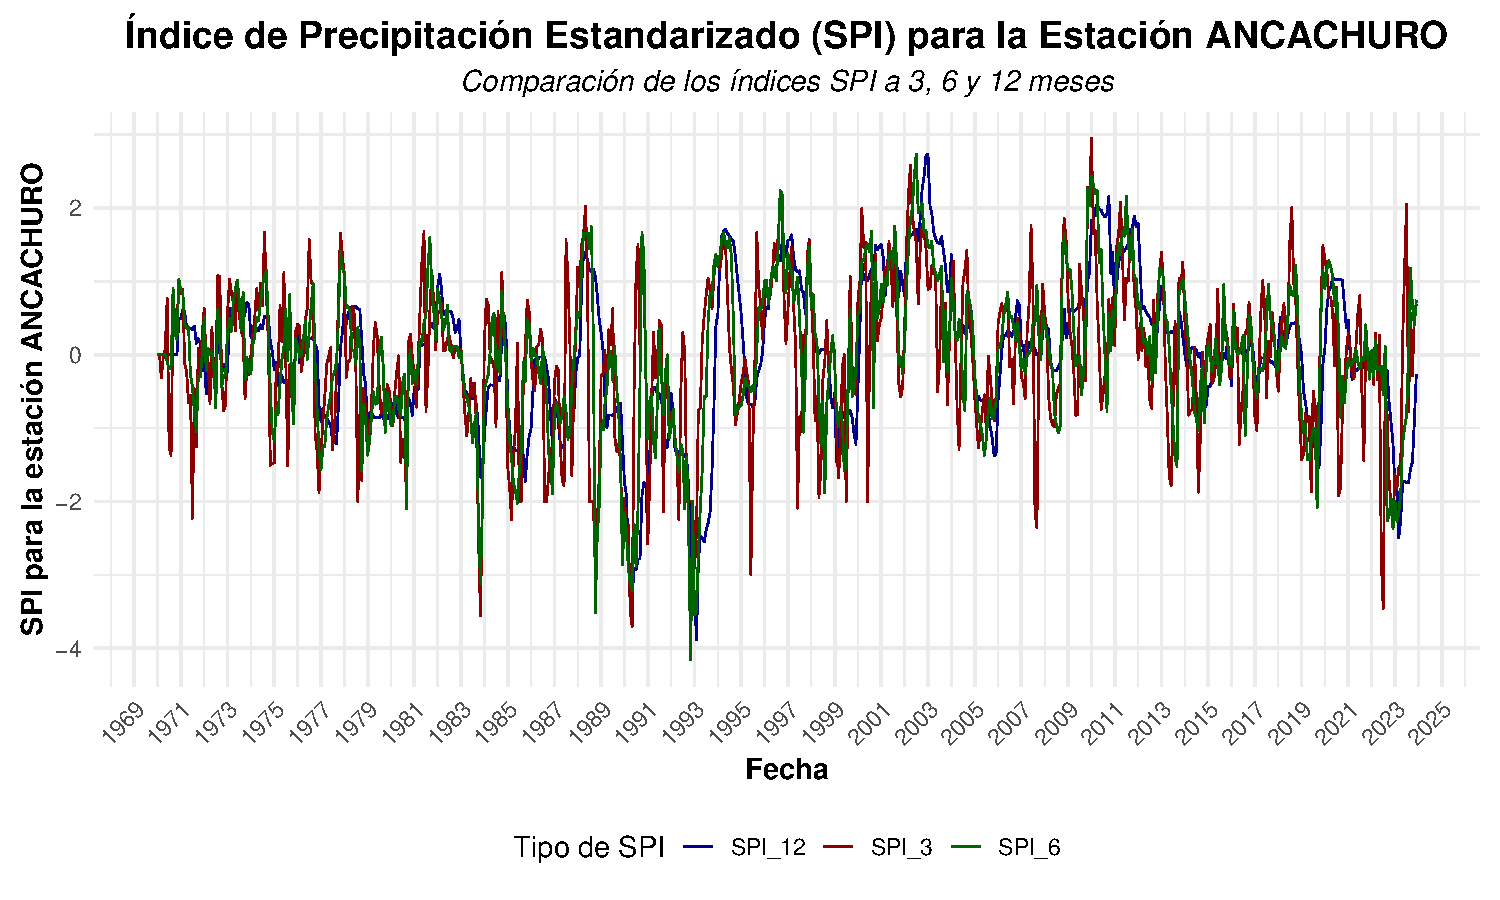
\includegraphics[width=\linewidth]{Capitulos/spi/SPI_Station_ANCACHURO.pdf}
    
\end{minipage} \hfill
\begin{minipage}{0.45\textwidth}
    \centering
    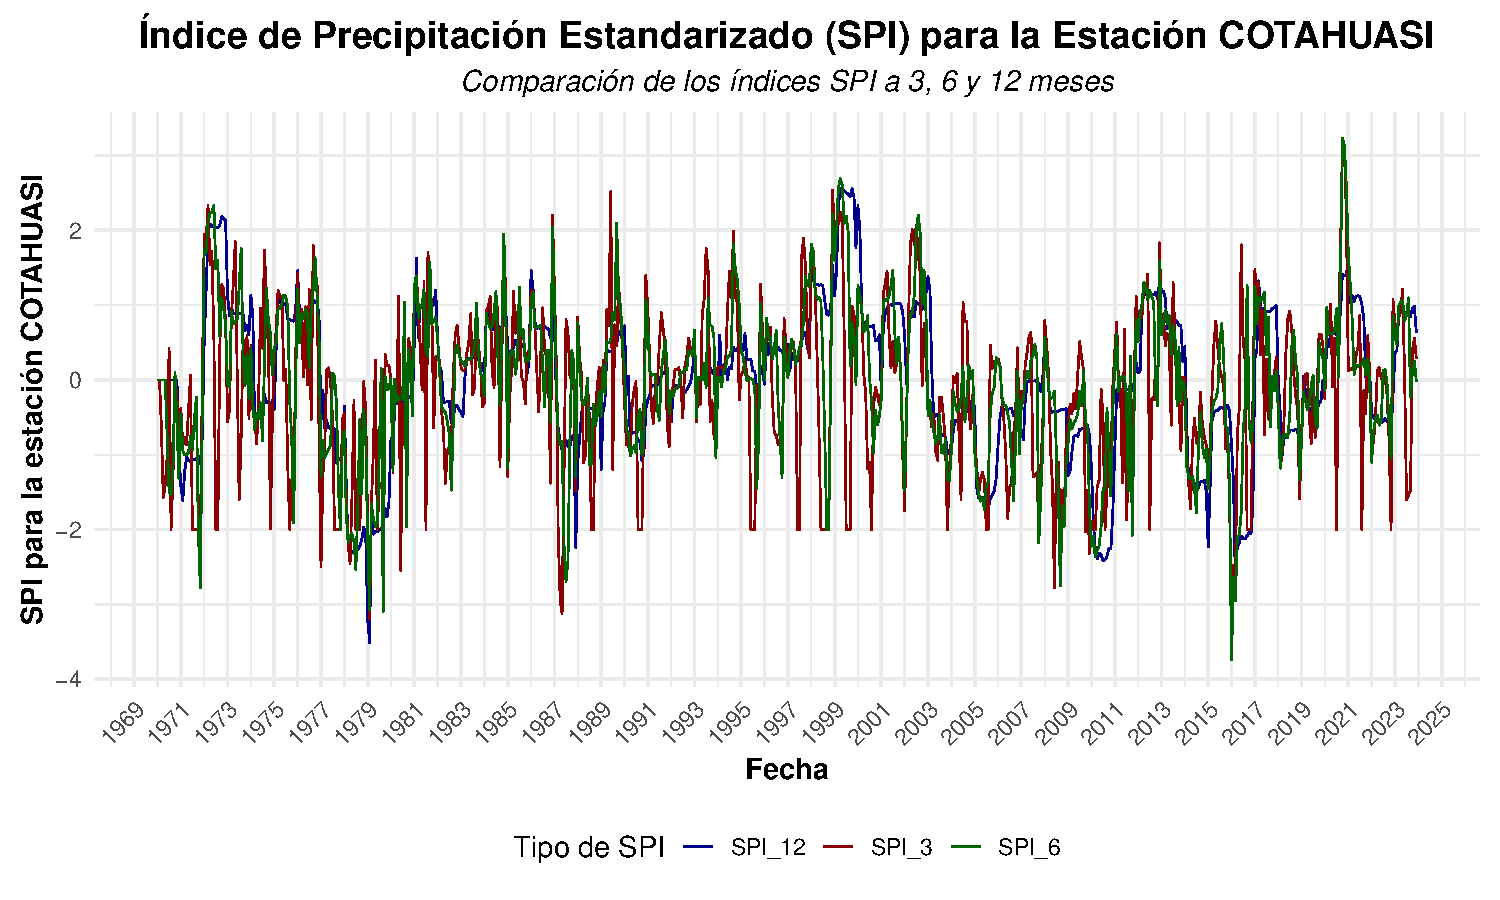
\includegraphics[width=\linewidth]{Capitulos/spi/SPI_Station_COTAHUASI.pdf}
   
\end{minipage} \hfill
\begin{minipage}{0.45\textwidth}
    \centering
    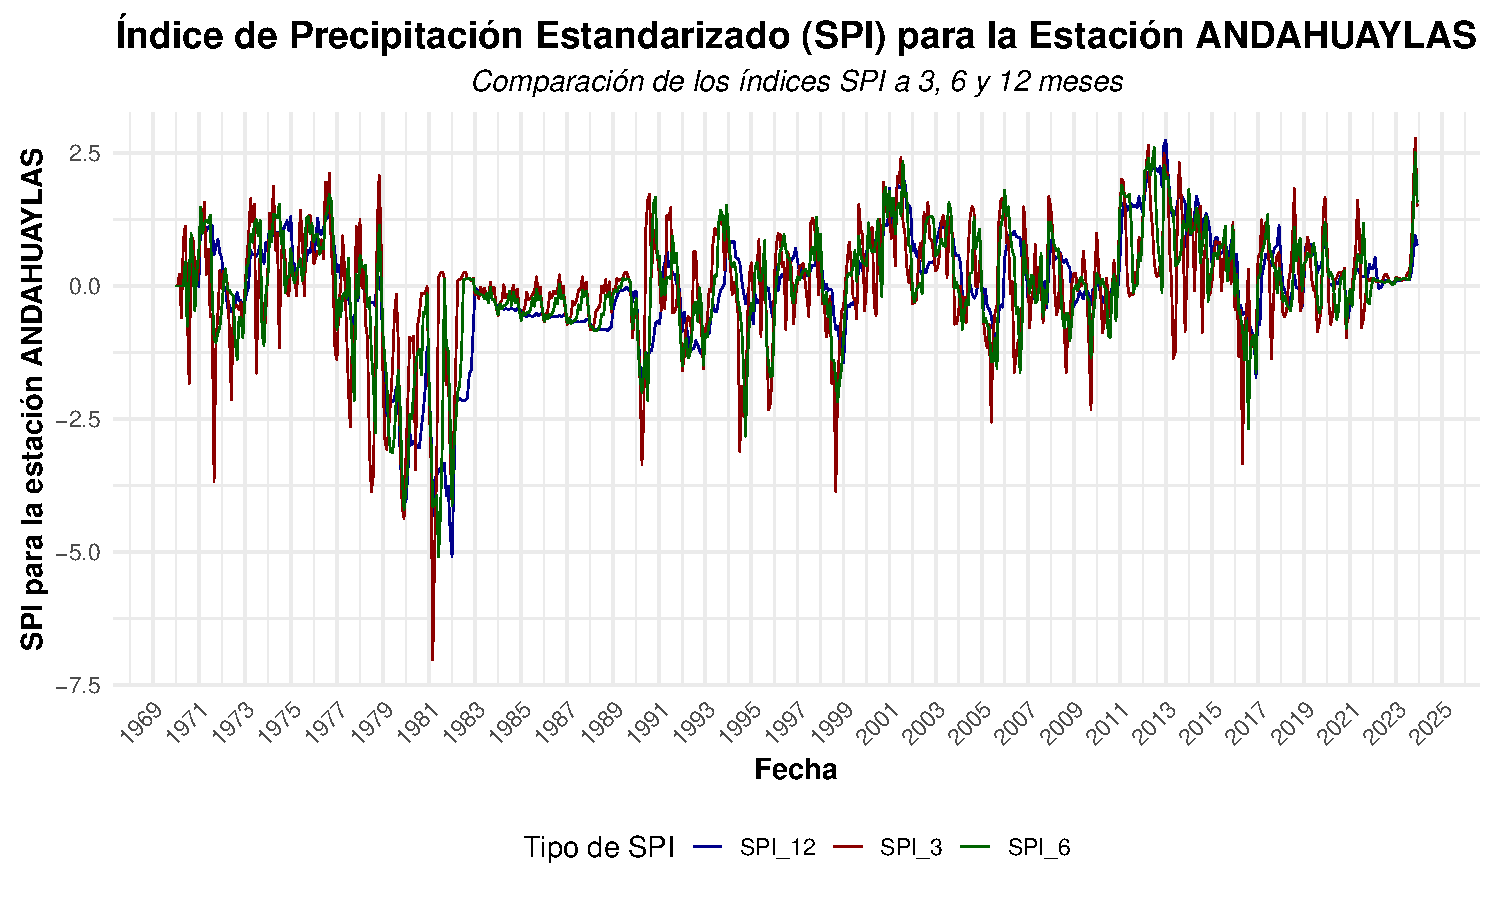
\includegraphics[width=\linewidth]{Capitulos/spi/SPI_Station_ANDAHUAYLAS.pdf}
  
\end{minipage}

\vskip\baselineskip  % Espacio entre filas de subgráficas

% Segunda fila de gráficas
\begin{minipage}{0.45\textwidth}
    \centering
    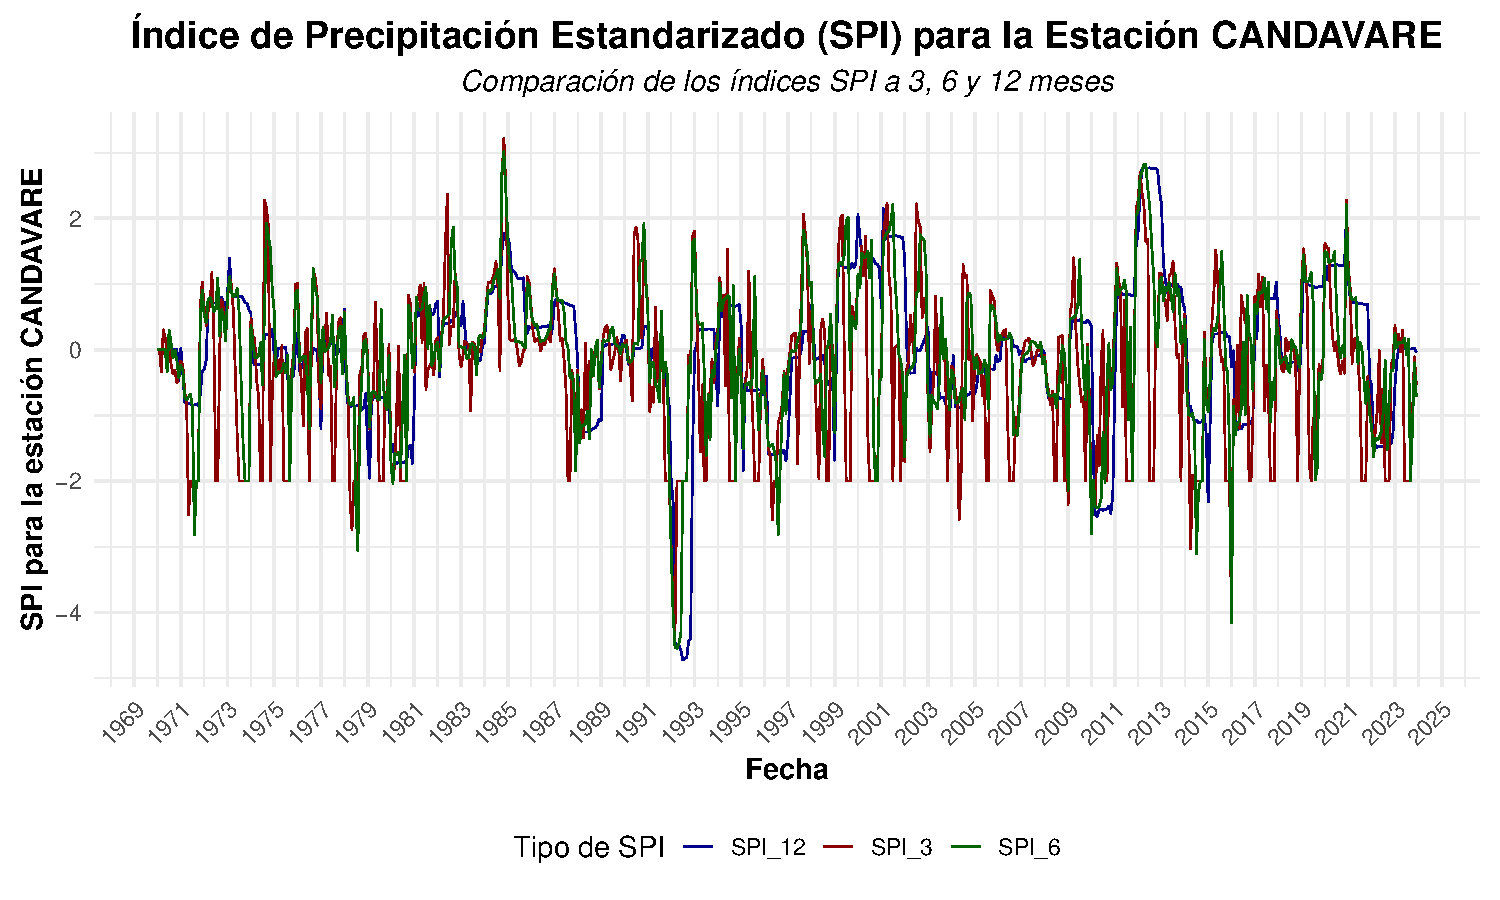
\includegraphics[width=\linewidth]{Capitulos/spi/SPI_Station_CANDAVARE.pdf}
   
\end{minipage} \hfill
\begin{minipage}{0.45\textwidth}
    \centering
    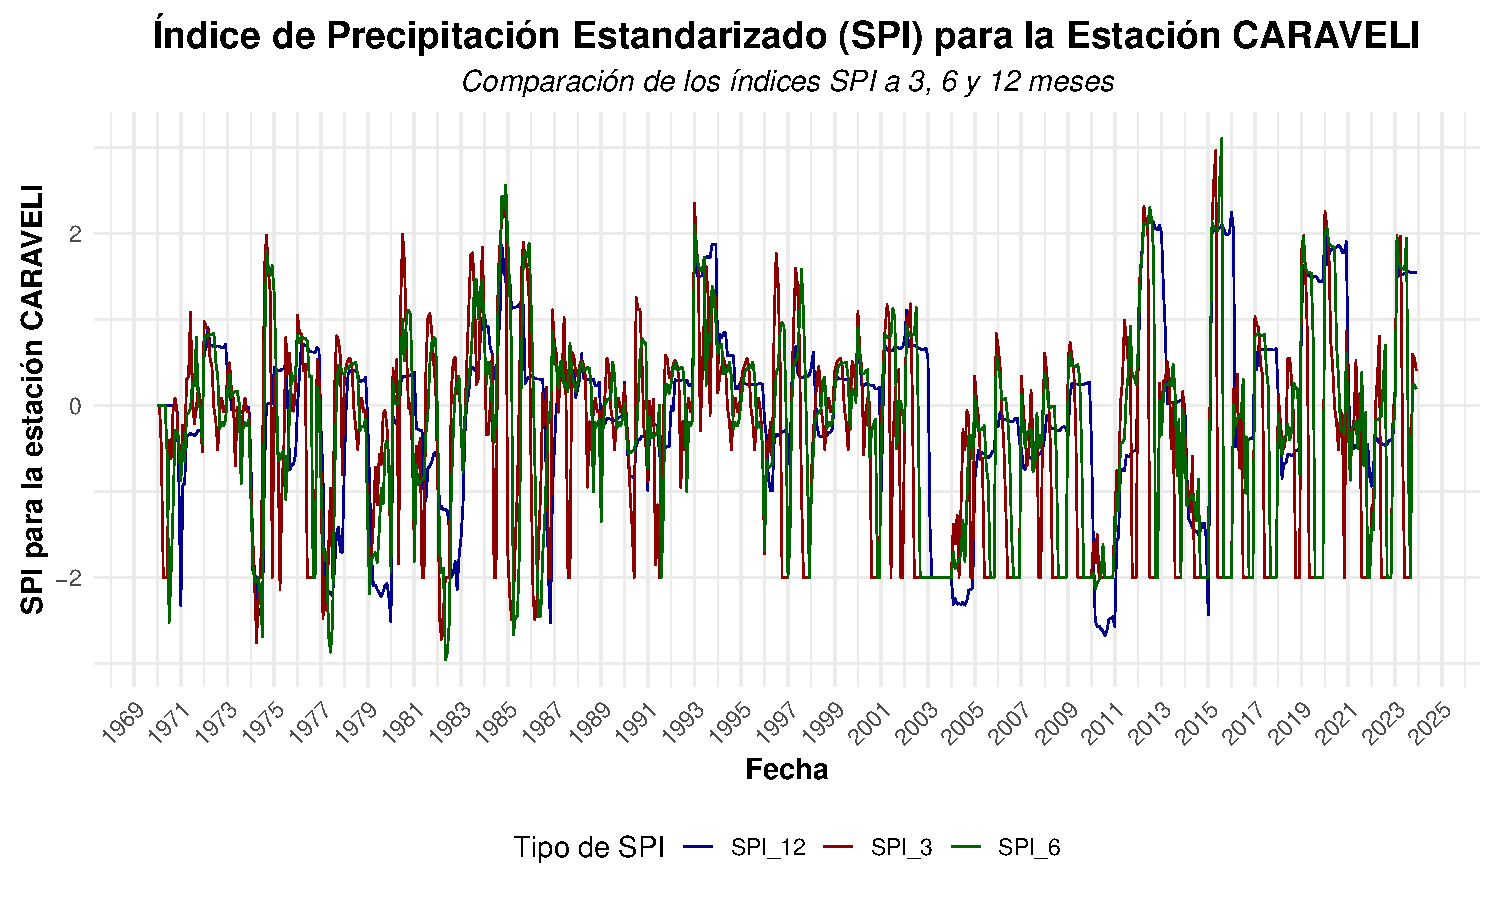
\includegraphics[width=\linewidth]{Capitulos/spi/SPI_Station_CARAVELI.pdf}
    
\end{minipage} \hfill
\begin{minipage}{0.45\textwidth}
    \centering
    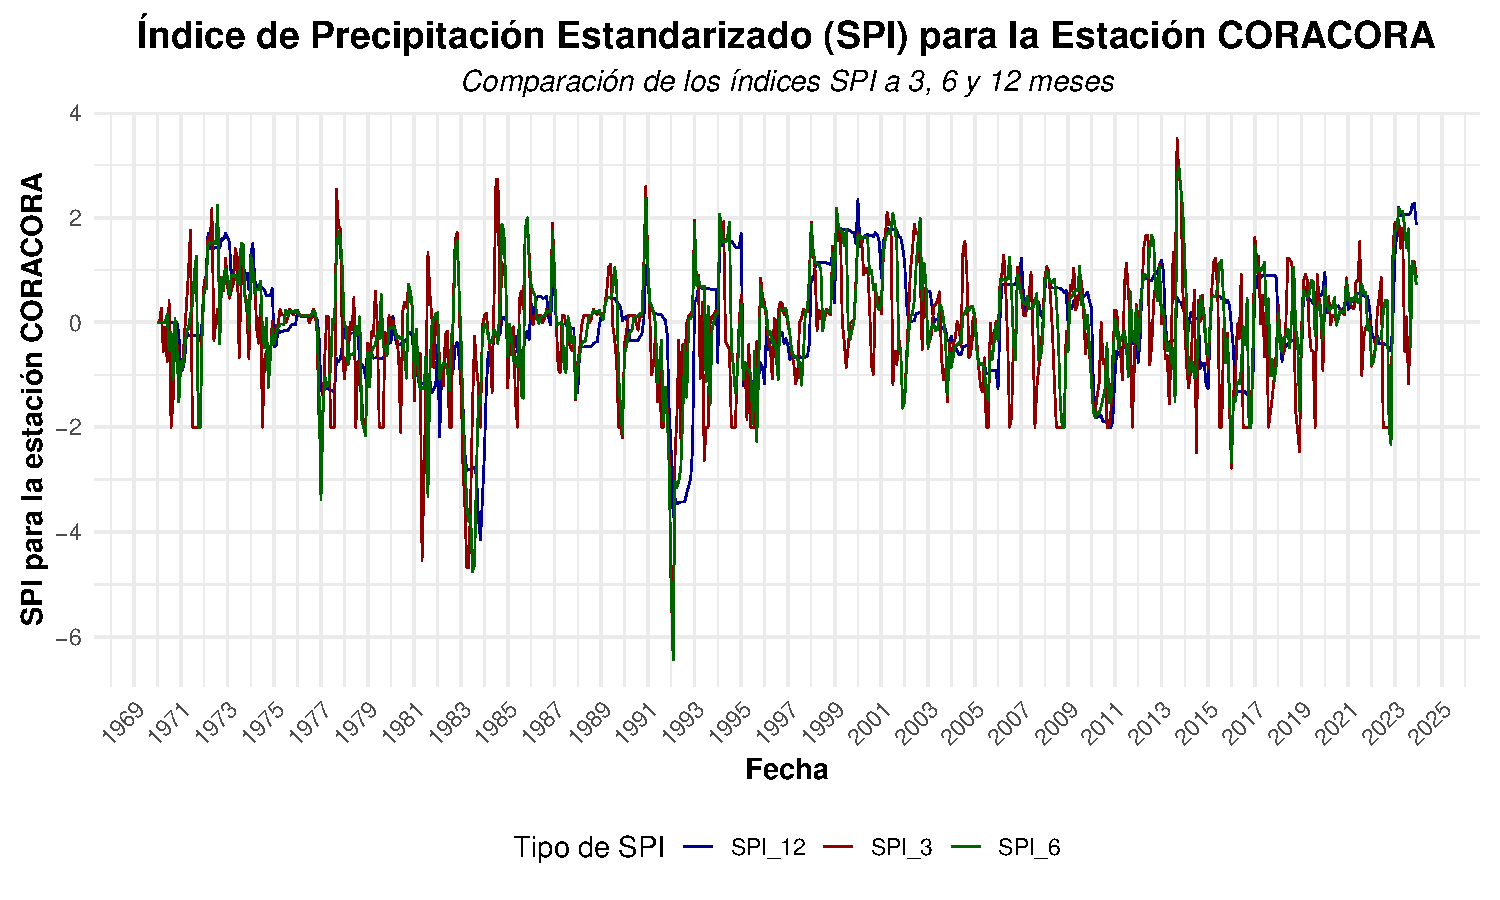
\includegraphics[width=\linewidth]{Capitulos/spi/SPI_Station_CORACORA.pdf}
   
\end{minipage}

\vskip\baselineskip  % Espacio entre filas de subgráficas

% Tercera fila de gráficas
\begin{minipage}{0.45\textwidth}
    \centering
    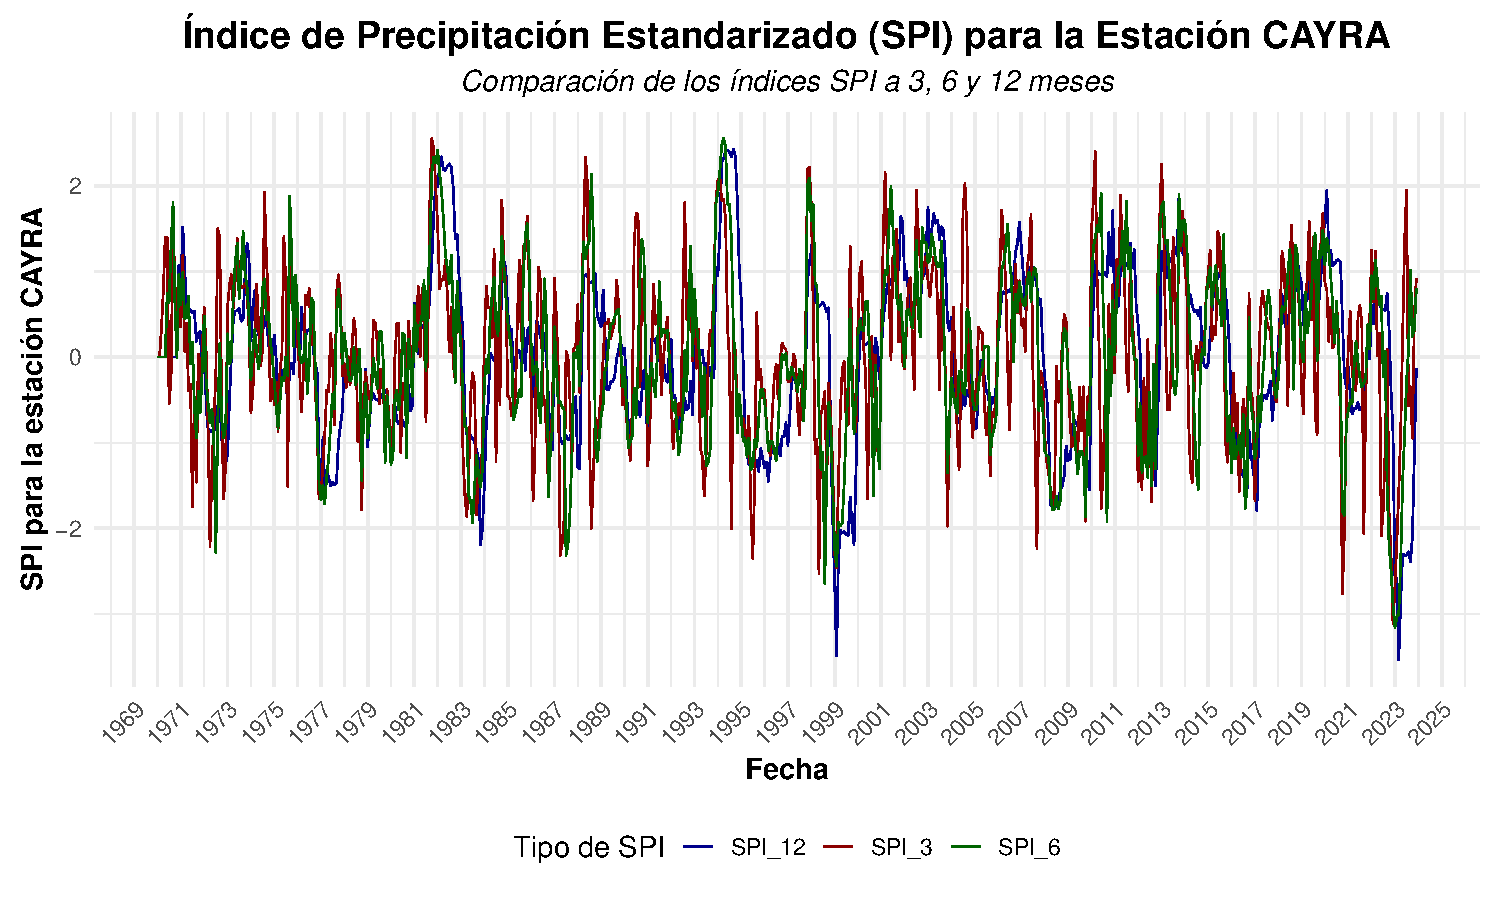
\includegraphics[width=\linewidth]{Capitulos/spi/SPI_Station_CAYRA.pdf}
    
\end{minipage} \hfill
\begin{minipage}{0.45\textwidth}
    \centering
    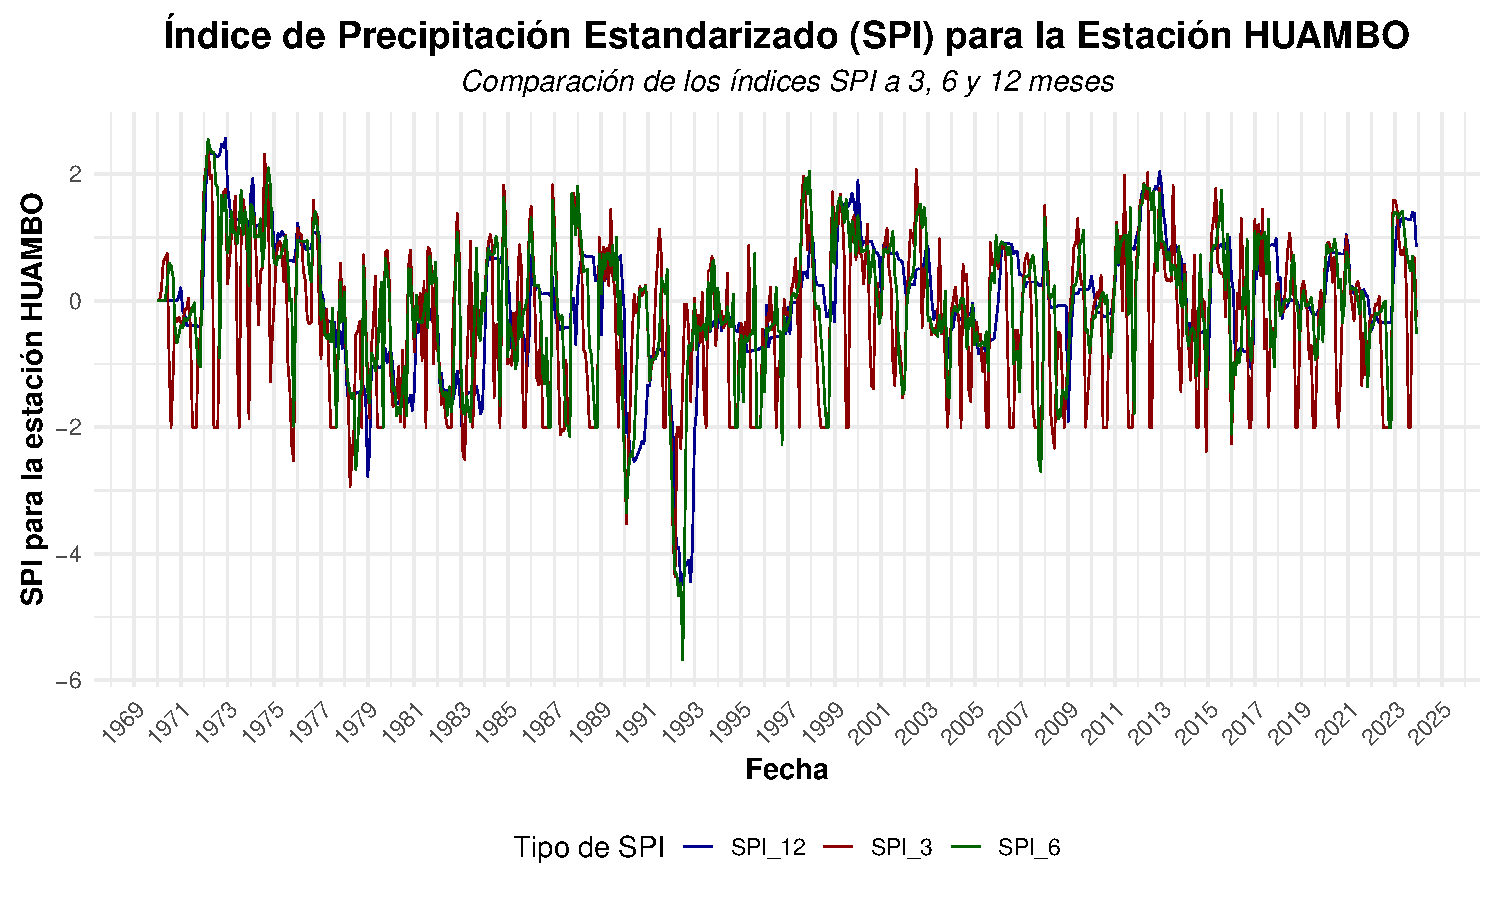
\includegraphics[width=\linewidth]{Capitulos/spi/SPI_Station_HUAMBO.pdf}
   
\end{minipage} \hfill
\begin{minipage}{0.45\textwidth}
    \centering
    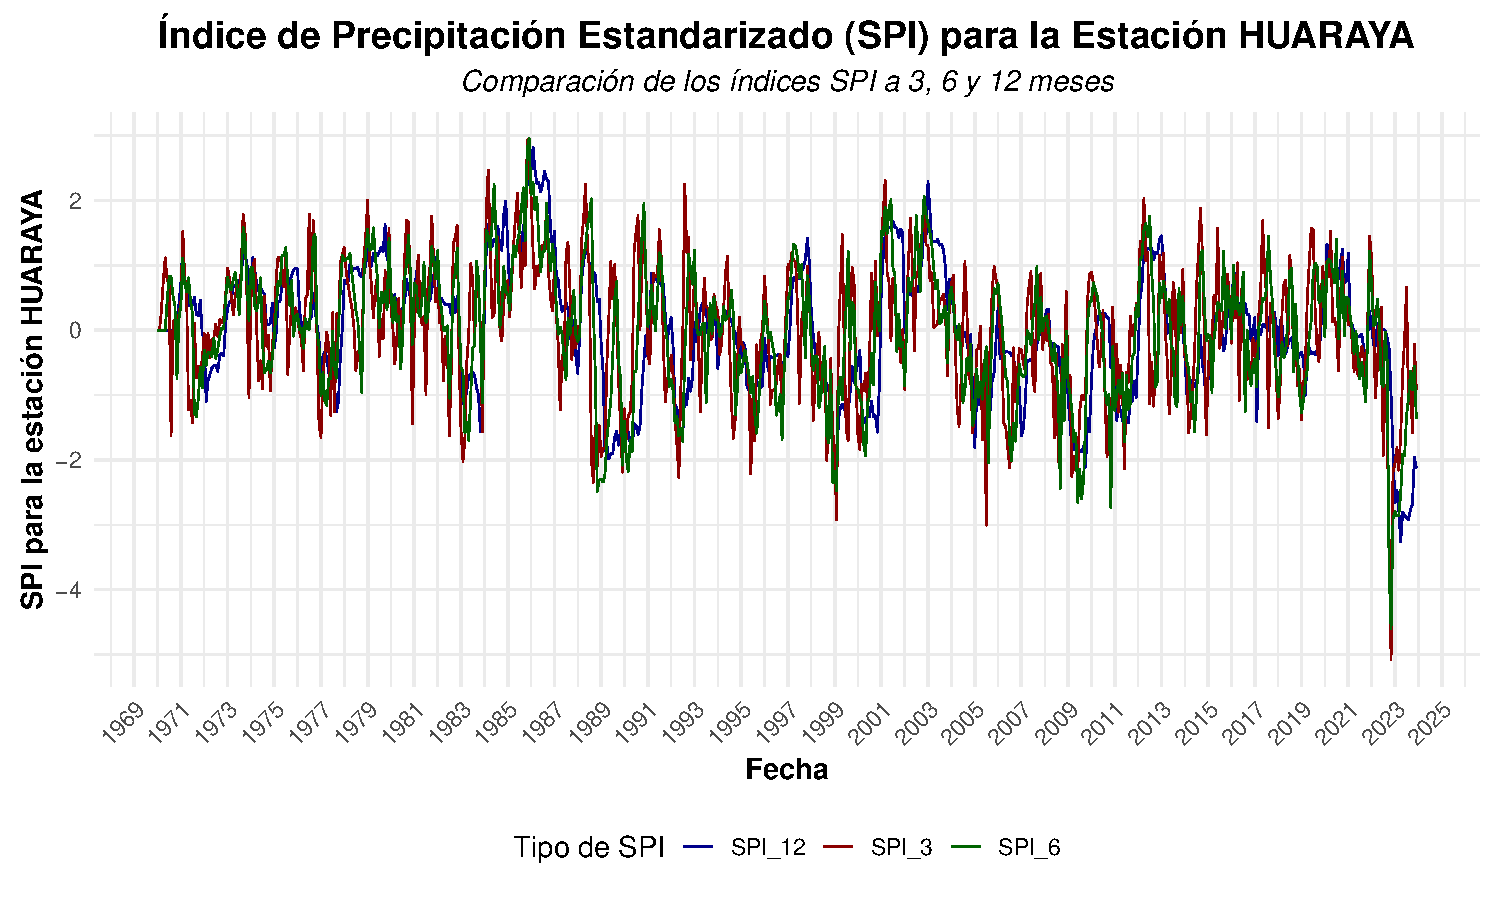
\includegraphics[width=\linewidth]{Capitulos/spi/SPI_Station_HUARAYA.pdf}
   
\end{minipage}

\vskip\baselineskip  % Espacio entre filas de subgráficas

% Cuarta fila de gráficas
\begin{minipage}{0.45\textwidth}
    \centering
    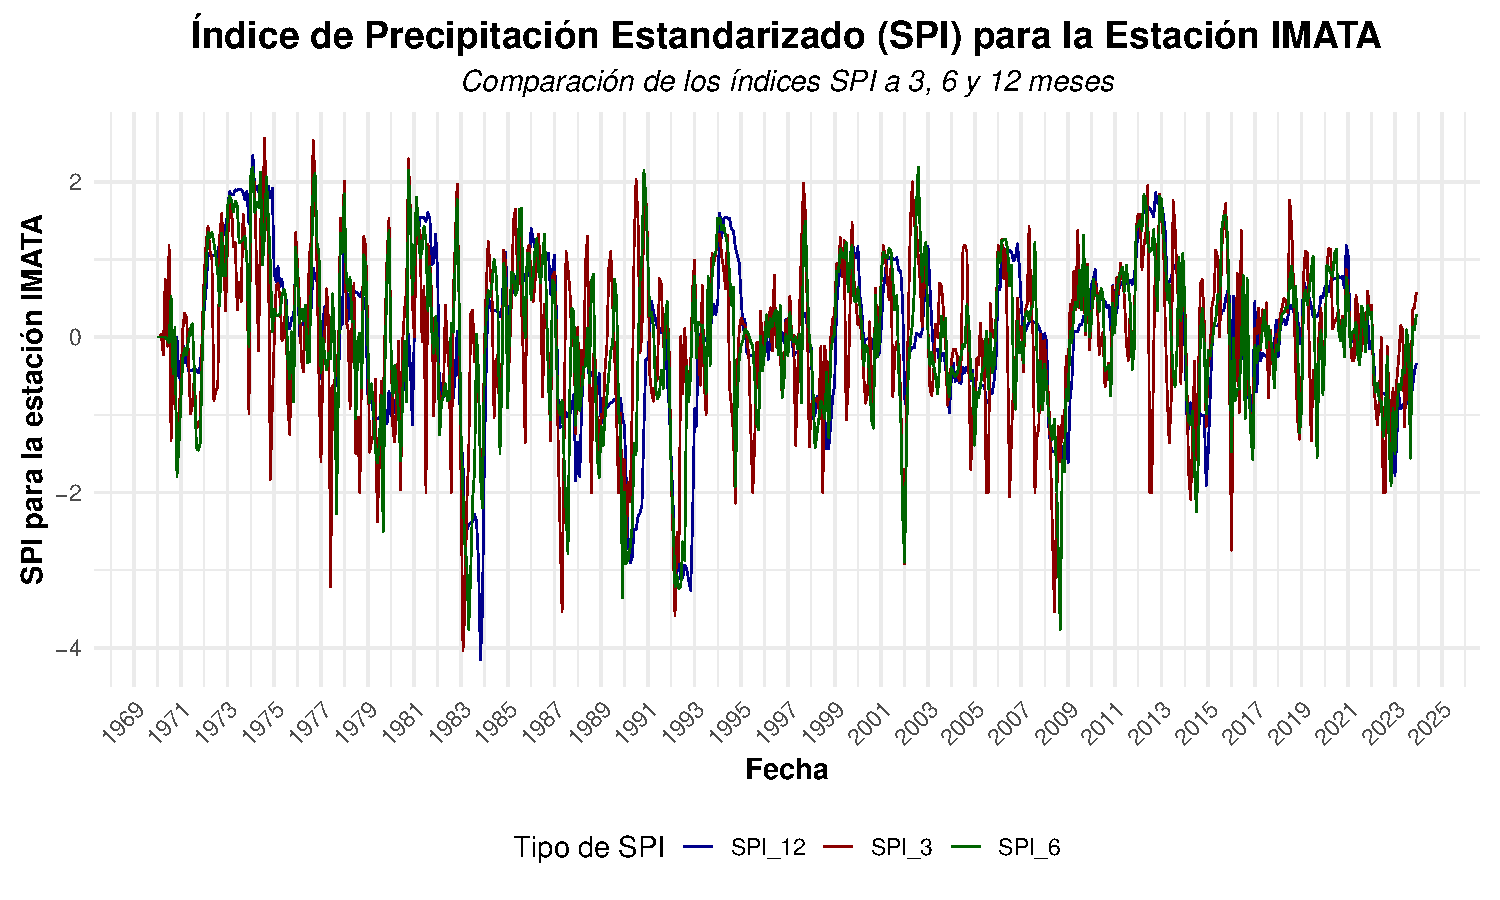
\includegraphics[width=\linewidth]{Capitulos/spi/SPI_Station_IMATA.pdf}
   
\end{minipage} \hfill
\begin{minipage}{0.45\textwidth}
    \centering
    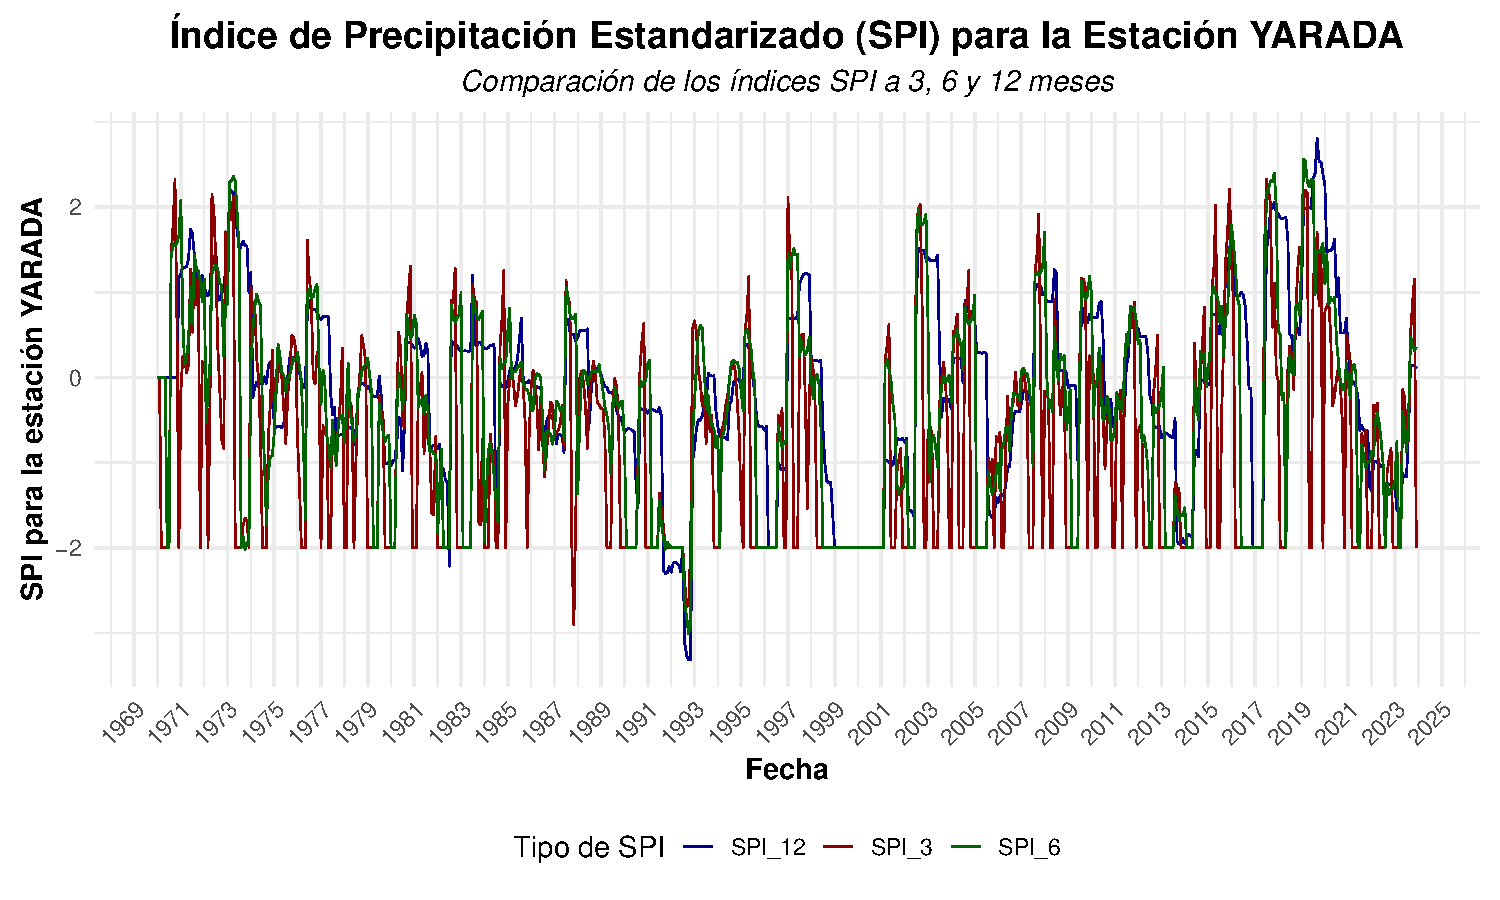
\includegraphics[width=\linewidth]{Capitulos/spi/SPI_Station_YARADA.pdf}
    
\end{minipage} \hfill
\begin{minipage}{0.45\textwidth}
    \centering
    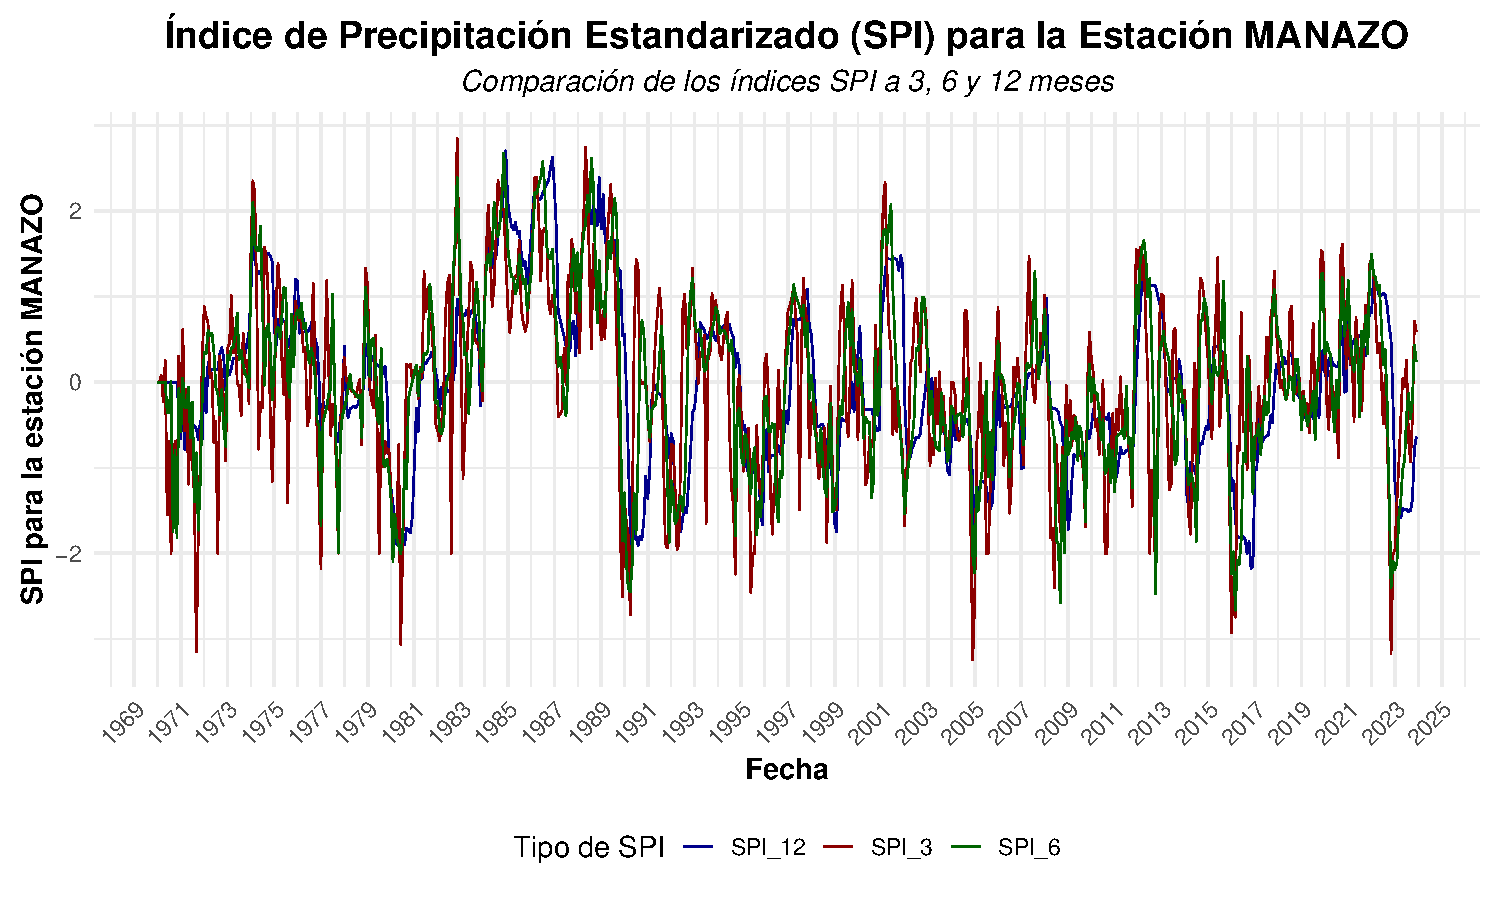
\includegraphics[width=\linewidth]{Capitulos/spi/SPI_Station_MANAZO.pdf}
   
\end{minipage}

\end{figure}
\end{landscape}

% Página 2
\begin{landscape}  % Continuar con orientación horizontal

\begin{figure}[h!]
\centering
% Quinta fila de gráficas
\begin{minipage}{0.45\textwidth}
    \centering
    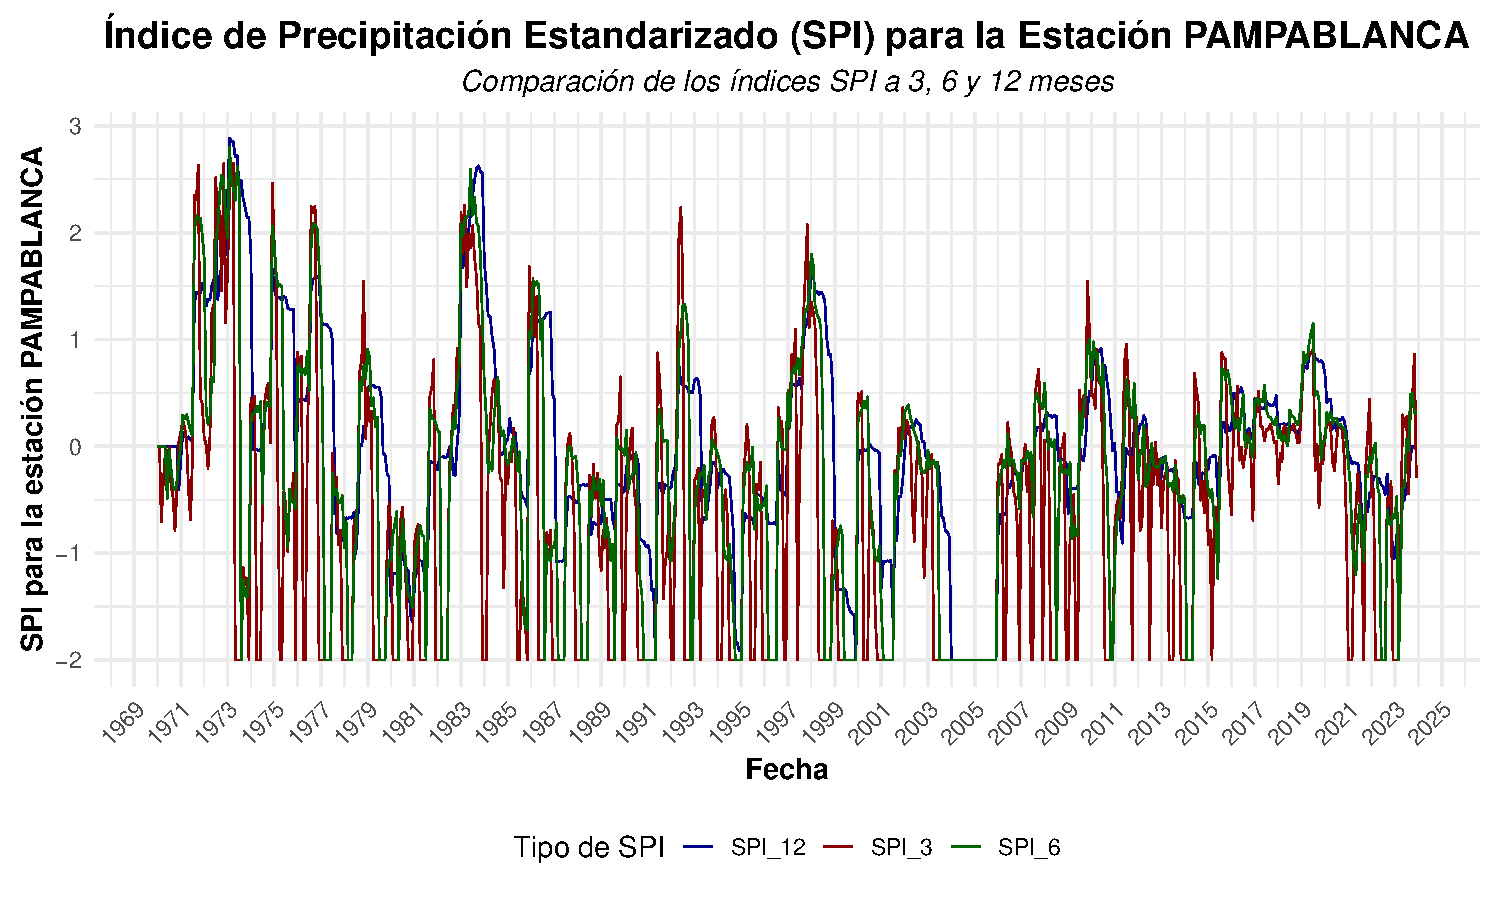
\includegraphics[width=\linewidth]{Capitulos/spi/SPI_Station_PAMPABLANCA.pdf}
  
\end{minipage} \hfill
\begin{minipage}{0.45\textwidth}
    \centering
    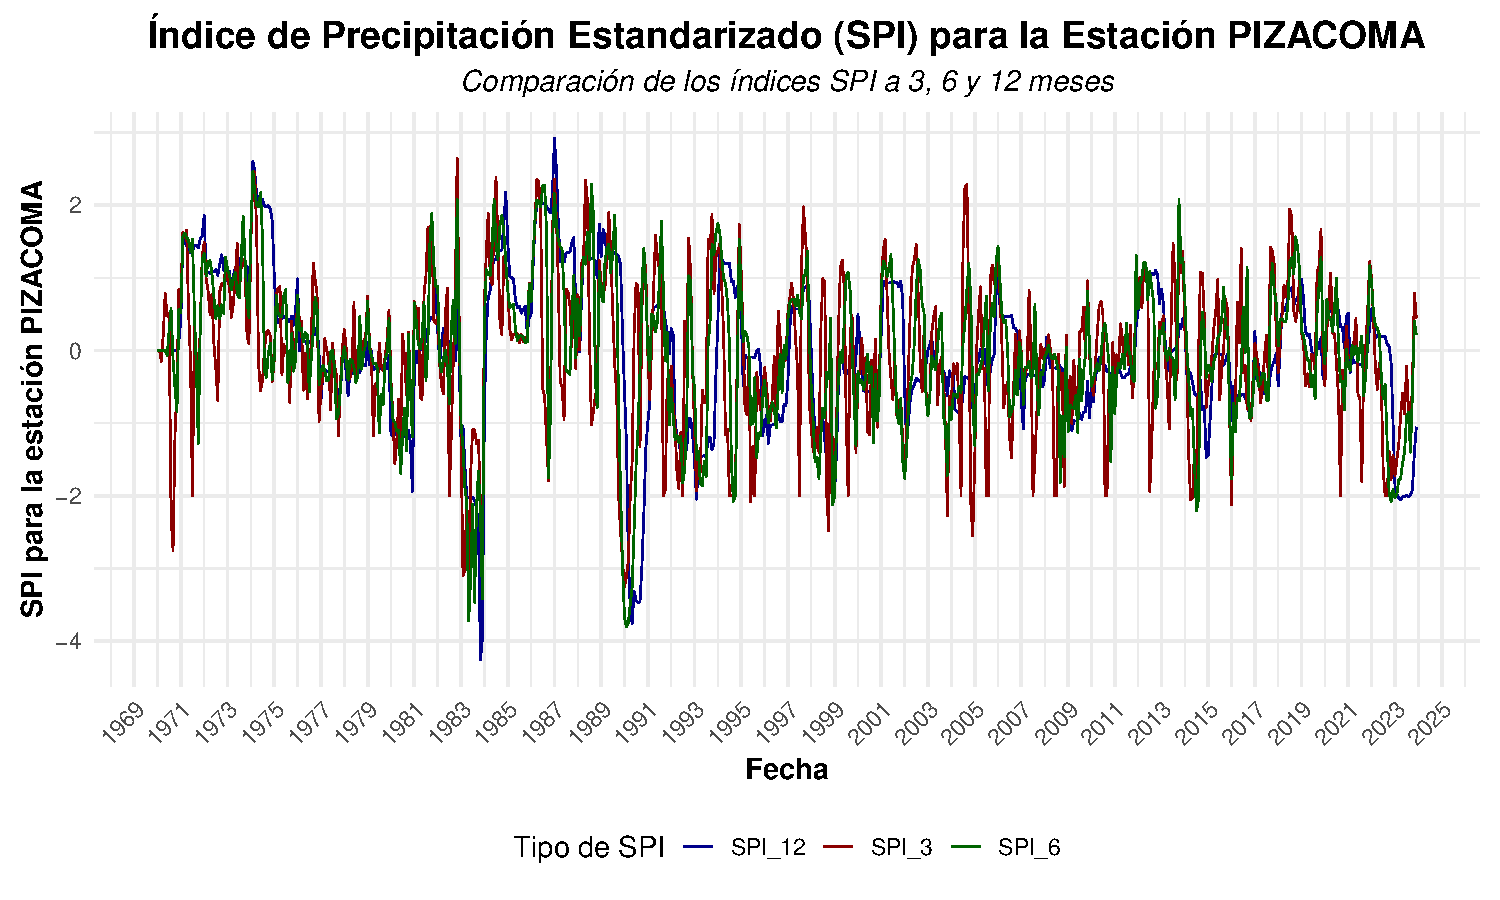
\includegraphics[width=\linewidth]{Capitulos/spi/SPI_Station_PIZACOMA.pdf}
    
\end{minipage} \hfill
\begin{minipage}{0.45\textwidth}
    \centering
    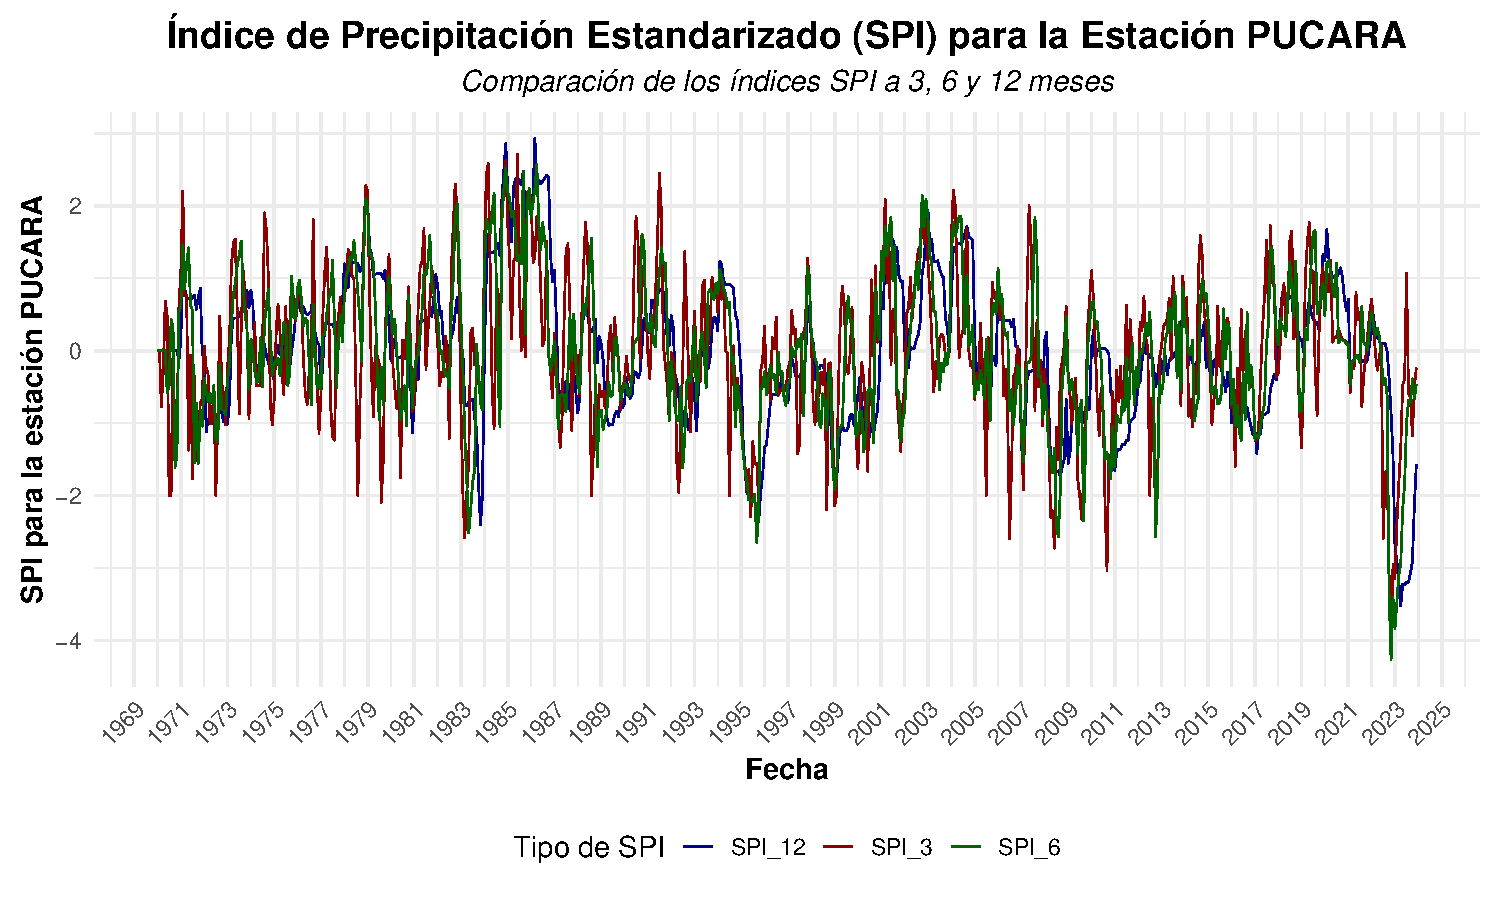
\includegraphics[width=\linewidth]{Capitulos/spi/SPI_Station_PUCARA.pdf}
   
\end{minipage}

\vskip\baselineskip  % Espacio entre filas de subgráficas

% Sexta fila de gráficas
\begin{minipage}{0.45\textwidth}
    \centering
    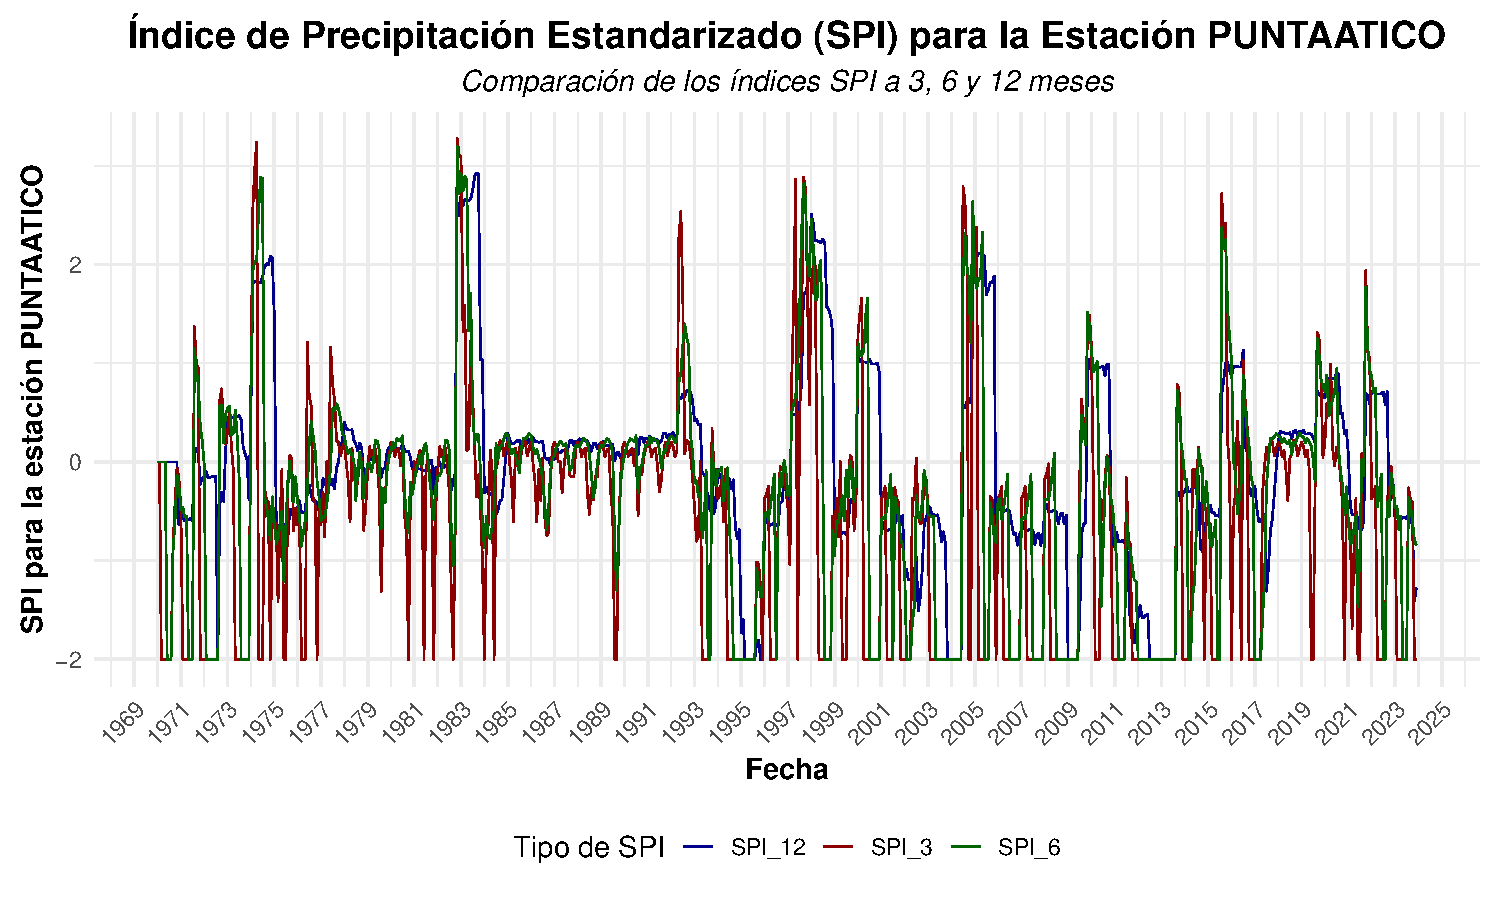
\includegraphics[width=\linewidth]{Capitulos/spi/SPI_Station_PUNTAATICO.pdf}
   
\end{minipage} \hfill
\begin{minipage}{0.45\textwidth}
    \centering
    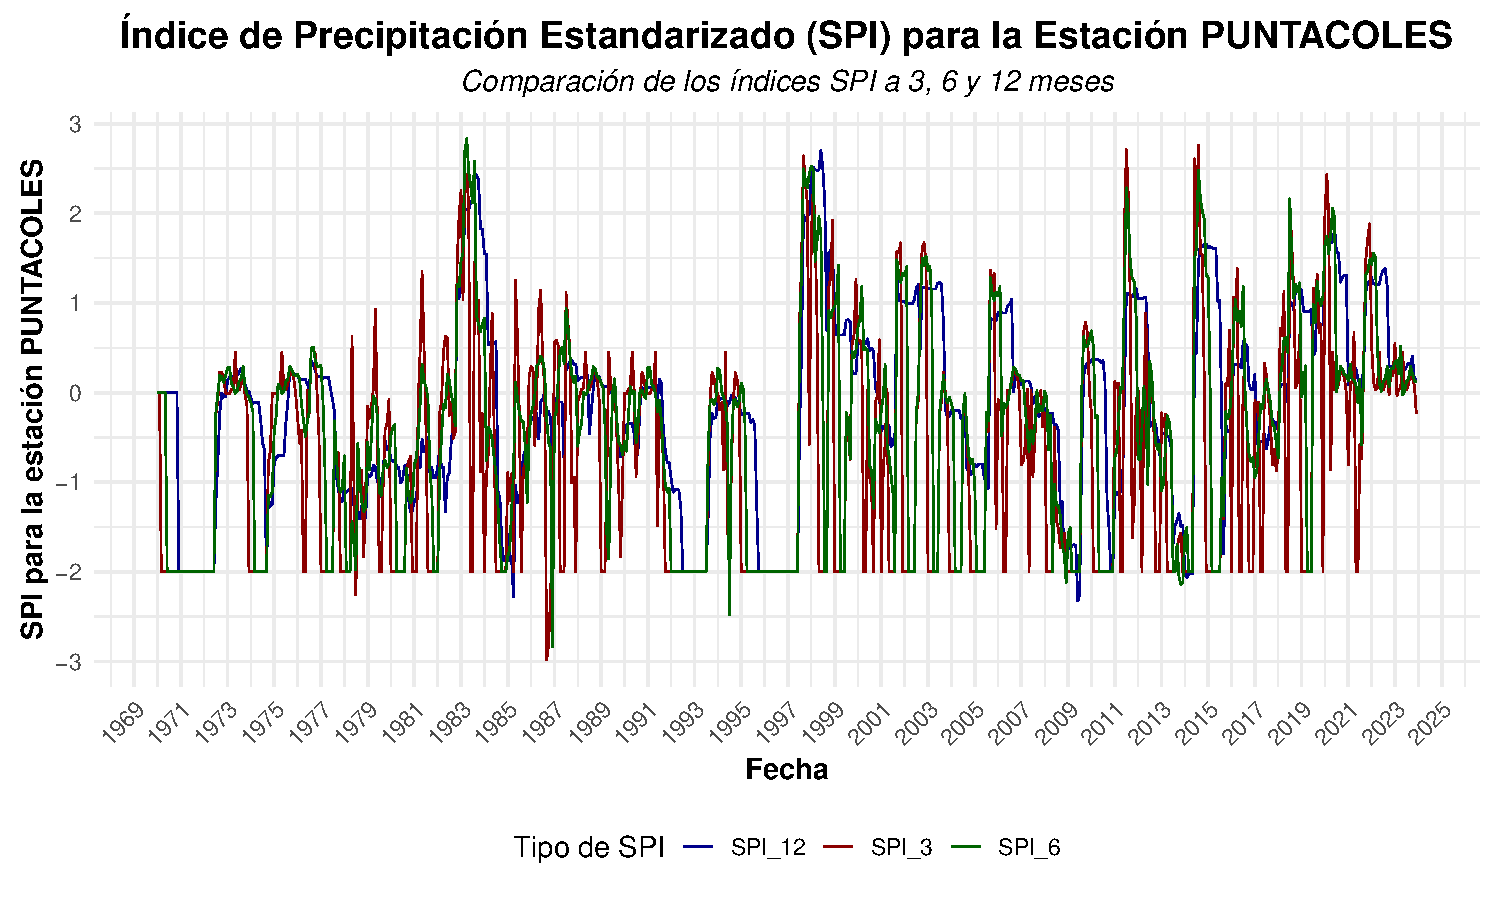
\includegraphics[width=\linewidth]{Capitulos/spi/SPI_Station_PUNTACOLES.pdf}
   
\end{minipage} \hfill
\begin{minipage}{0.45\textwidth}
    \centering
    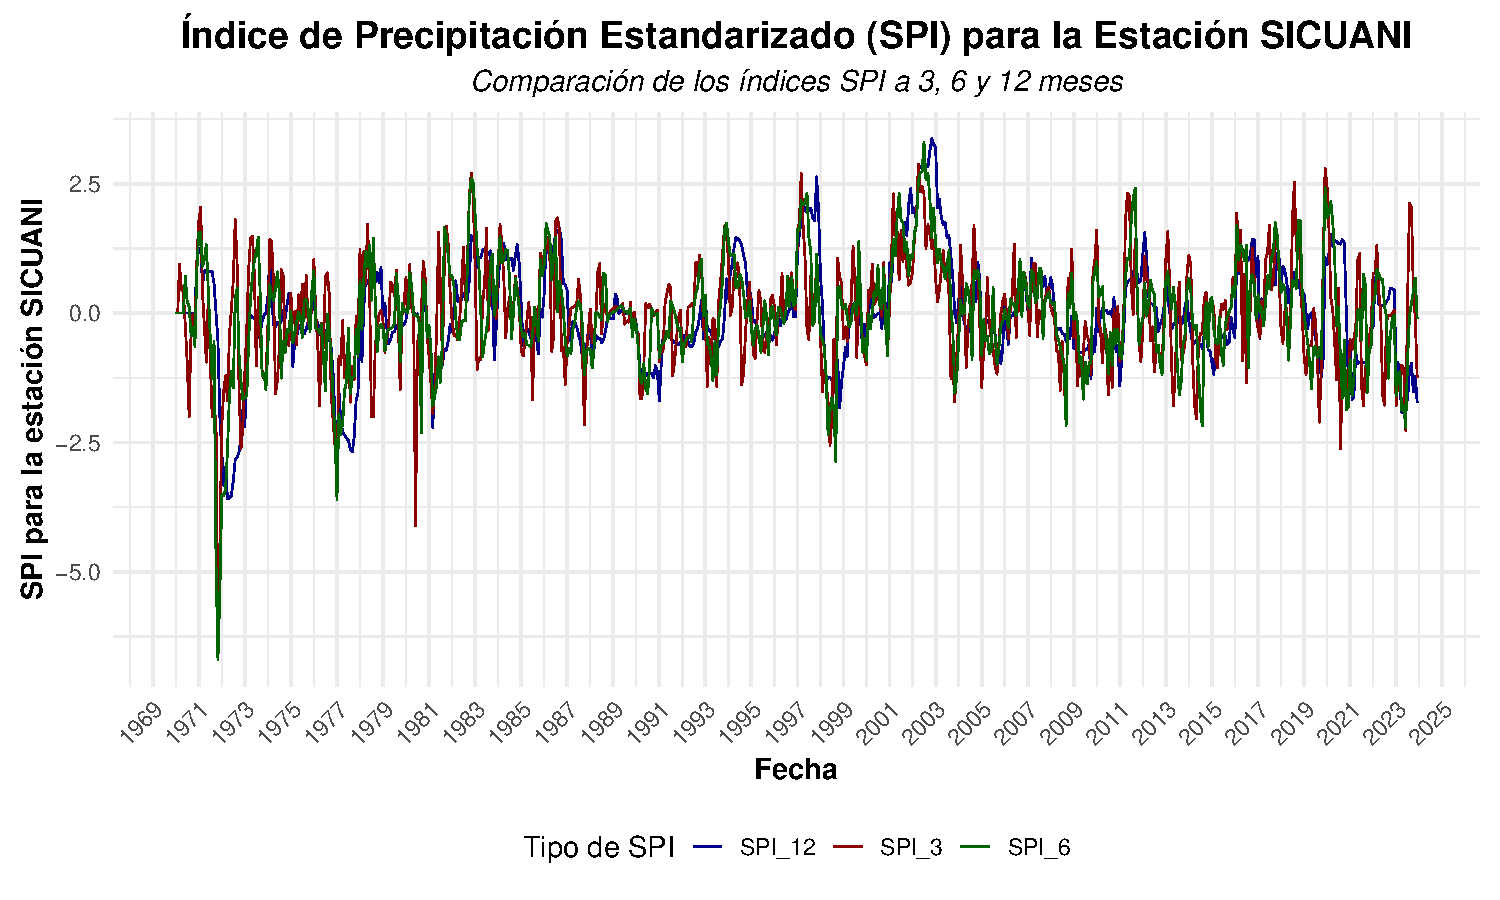
\includegraphics[width=\linewidth]{Capitulos/spi/SPI_Station_SICUANI.pdf}
   
\end{minipage}

\vskip\baselineskip  % Espacio entre filas de subgráficas

% Séptima fila de gráficas
\begin{minipage}{0.45\textwidth}
    \centering
    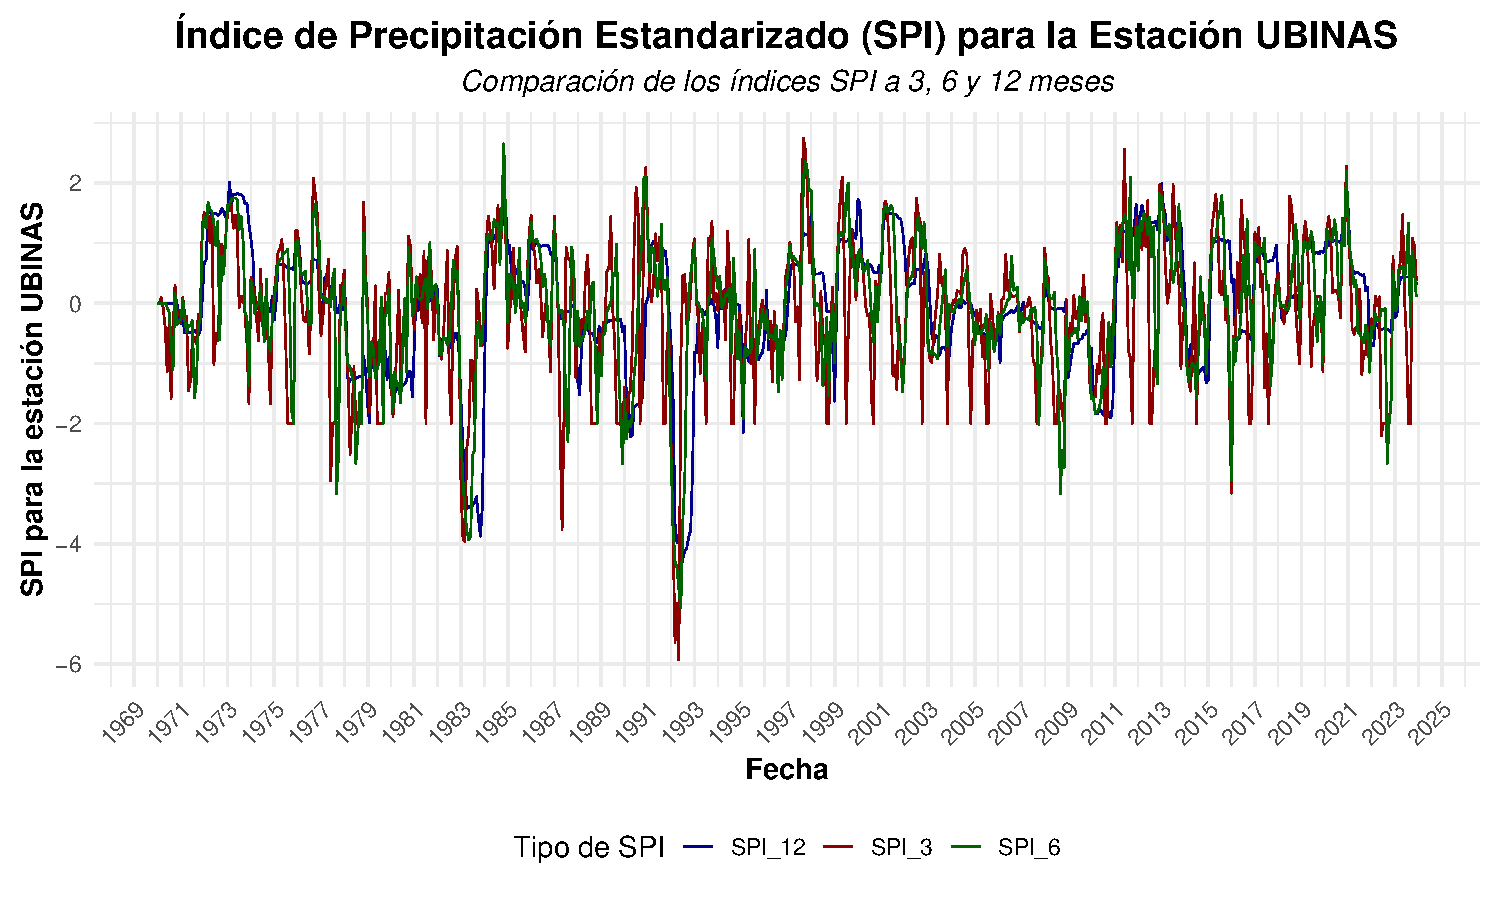
\includegraphics[width=\linewidth]{Capitulos/spi/SPI_Station_UBINAS.pdf}
 
\end{minipage}
\end{figure}

\end{landscape}

\subsection{Análisis de los Índices SPI para las Estaciones}


\subsection*{Estación \textit{ANCACHURO}}

La gráfica para la estación \textit{ANCACHURO} muestra la variabilidad de las precipitaciones a través de los tres índices SPI (3, 6 y 12 meses). El SPI a 3 meses refleja fluctuaciones con períodos de **sequía moderada** seguidos de fases más húmedas. El SPI a 6 y 12 meses indican una tendencia más estable, con algunos períodos de sequía moderada, pero mayormente en la categoría **normal**.

\subsection*{Estación \textit{ANDAHUAYLAS}}

El gráfico para la estación \textit{ANDAHUAYLAS} muestra fluctuaciones en las precipitaciones, con el SPI a 3 meses alcanzando **condiciones de sequía moderada** en varios períodos. El SPI a 6 y 12 meses son más estables, aunque también muestran momentos de **sequía severa** y condiciones más húmedas en algunos intervalos.

\subsection*{Estación \textit{CANDAVARE}}

Para la estación \textit{CANDAVARE}, el gráfico muestra fluctuaciones de SPI en los tres períodos. El SPI a 3 meses tiene varios picos hacia **sequía moderada**, con algunos intervalos de humedad. El SPI a 6 y 12 meses son más estables, aunque presentan caídas hacia la zona de sequía moderada en ciertos momentos.

\subsection*{Estación \textit{CARAVELI}}

La estación \textit{CARAVELI} muestra una tendencia similar en los tres SPI, con picos hacia **sequía** en el SPI a 3 meses. El SPI a 6 y 12 meses presentan una variabilidad más moderada, pero también reflejan períodos secos, especialmente en los primeros años del gráfico.

\subsection*{Estación \textit{CAYRA}}

En la estación \textit{CAYRA}, el SPI a 3 meses refleja fluctuaciones significativas, con momentos de **sequía moderada** y **condiciones húmedas** intercaladas. El SPI a 6 meses tiene una tendencia más estable, mientras que el SPI a 12 meses muestra un comportamiento equilibrado, con períodos secos moderados seguidos de condiciones normales.

\subsection*{Estación \textit{CORACORA}}

El gráfico de la estación \textit{CORACORA} muestra fluctuaciones en los tres índices SPI. El SPI a 3 meses refleja varios períodos de **sequía severa**. El SPI a 6 y 12 meses también presentan caídas hacia la zona de sequía, pero la tendencia general es más estable, con algunos intervalos de humedad en el largo plazo.

\subsection*{Estación \textit{COTAHUASI}}

En la estación \textit{COTAHUASI}, el gráfico muestra un comportamiento variable en los tres períodos de SPI. El SPI a 3 meses presenta varios períodos de **sequía severa**, mientras que el SPI a 6 meses es más estable, pero también muestra fluctuaciones negativas. El SPI a 12 meses muestra una tendencia moderada, con algunos picos de sequía prolongada.

\subsection*{Estación \textit{HUAMBO}}

El gráfico de la estación \textit{HUAMBO} refleja fluctuaciones en los tres SPI, con algunos picos de **sequía severa** en el SPI a 3 meses. El SPI a 6 y 12 meses son más estables, pero presentan caídas hacia la categoría de sequía moderada, con algunos intervalos secos prolongados en la estación.

\subsection*{Estación \textit{HUARAYA}}

La estación \textit{HUARAYA} muestra fluctuaciones tanto en el SPI a 3 meses como en el SPI a 6 y 12 meses. El SPI a 3 meses refleja fluctuaciones hacia valores negativos, lo que indica **sequía moderada**. El SPI a 6 y 12 meses son más estables, aunque también muestran momentos secos, pero con una tendencia general más equilibrada.


\subsection*{Estación \textit{IMATA}}

La gráfica para la estación \textit{IMATA} muestra un comportamiento de las precipitaciones con fluctuaciones evidentes en los tres períodos de SPI. El SPI a 3 meses muestra picos negativos en los primeros años, lo que sugiere condiciones de **sequía severa**. El SPI a 6 y 12 meses refleja una tendencia más estable, pero también presenta valores negativos en algunas ocasiones, indicando sequía moderada y **condiciones húmedas** en ciertos períodos.

\subsection*{Estación \textit{MANAZO}}

El gráfico para la estación \textit{MANAZO} muestra un comportamiento variable en los tres índices SPI. El SPI a 3 meses tiene fluctuaciones hacia los valores negativos, lo que indica **sequía**. El SPI a 6 meses es más estable, pero también presenta caídas a valores negativos. El SPI a 12 meses muestra una tendencia equilibrada, con algunos períodos de **sequía severa** y otros más húmedos.

\subsection*{Estación \textit{PAMPABLANCA}}

La estación \textit{PAMPABLANCA} muestra en su gráfico un comportamiento más seco, con picos negativos en los tres períodos de SPI. El SPI a 3 meses refleja **sequía severa**, especialmente en los primeros años. El SPI a 6 y 12 meses también presentan valores negativos, lo que sugiere que la estación experimentó **sequías prolongadas** en la mayor parte del tiempo.

\subsection*{Estación \textit{PIZACOMA}}

En la estación \textit{PIZACOMA}, el SPI de 3 meses refleja fluctuaciones significativas, con algunos picos en valores negativos. El SPI a 6 y 12 meses son más estables, pero también muestran intervalos de **sequía moderada**. En general, la estación experimentó períodos secos intercalados con condiciones más normales.

\subsection*{Estación \textit{PUCARA}}

La gráfica para la estación \textit{PUCARA} muestra un comportamiento más estable en el SPI a 6 y 12 meses, mientras que el SPI a 3 meses muestra algunas fluctuaciones significativas. El SPI a 6 y 12 meses indican **condiciones normales** en la mayoría del tiempo, con solo algunos episodios más secos, aunque con una tendencia positiva en los últimos años.

\subsection*{Estación \textit{PUNTAATICO}}

El gráfico para la estación \textit{PUNTAATICO} refleja fluctuaciones en las precipitaciones con los tres índices SPI. El SPI a 3 meses muestra un comportamiento variable, con varios períodos de **sequía moderada**. El SPI a 6 meses es más estable, pero con algunas caídas hacia valores negativos. El SPI a 12 meses muestra una tendencia más equilibrada, con algunos picos hacia **condiciones húmedas**.

\subsection*{Estación \textit{PUNTACOLES}}

Para la estación \textit{PUNTACOLES}, el gráfico muestra fluctuaciones en los tres períodos de SPI. El SPI a 3 meses presenta **sequía severa** en varios períodos, mientras que el SPI a 6 y 12 meses muestran una tendencia más equilibrada. La estación experimenta algunos momentos de sequía, pero también fases más húmedas.

\subsection*{Estación \textit{SICUANI}}

En la estación \textit{SICUANI}, el gráfico muestra fluctuaciones en el SPI a 3 meses, con algunos períodos de **sequía** y condiciones normales. El SPI a 6 meses es más estable, con algunos picos hacia valores negativos. El SPI a 12 meses muestra una tendencia más equilibrada, con intervalos secos intercalados con condiciones húmedas.

\subsection*{Estación \textit{UBINAS}}

Para la estación \textit{UBINAS}, el gráfico muestra una tendencia variable en los tres índices SPI. El SPI a 3 meses muestra algunos picos de **sequía severa**, especialmente hacia el final del período. El SPI a 6 y 12 meses presentan una tendencia más estable, con intervalos de **sequía moderada** seguidos de valores cercanos a lo normal.

\subsection*{Estación \textit{YARADA}}

El gráfico para la estación \textit{YARADA} muestra fluctuaciones en el SPI a 3 meses, con algunos picos de sequía, seguidos de algunos intervalos más húmedos. El SPI a 6 y 12 meses tiene una tendencia más estable, pero también presenta caídas hacia valores negativos, lo que indica episodios de **sequía moderada** y otras condiciones más húmedas.

\section{Análisis de Cópulas Bivariadas}

El análisis de cópulas bivariadas tiene como objetivo modelar la dependencia y la correlación entre las variables consideradas, en este caso, entre los índices de precipitación estandarizados (SPI) y otras variables climáticas, como la humedad relativa, la precipitación y la velocidad media del viento. Antes de realizar la construcción de cópulas bivariadas, es necesario llevar a cabo una serie de pasos preliminares que aseguren la adecuada integración y análisis de los datos.

En primer lugar, se debe realizar una **transformación de los datos** para que todas las variables involucradas estén en un formato adecuado para el análisis de cópulas. Esto implica la **normalización** de los datos para que las distribuciones de las variables sean independientes de las unidades de medida y, en muchos casos, sea necesario aplicar alguna **transformación marginal** para que las variables sigan distribuciones conocidas, como la distribución uniforme o normal.

Una vez que los datos han sido preprocesados y transformados adecuadamente, el siguiente paso es analizar la **dependencia bivariada** entre los índices SPI y las variables climáticas, como la **humedad relativa**, la **precipitación** y la **velocidad media del viento**. En este paso, se explora la **relación entre dos variables** a través del uso de cópulas bivariadas, que son herramientas estadísticas muy útiles para modelar la dependencia no lineal y explorar el tipo de relación entre las variables.

Las cópulas bivariadas permiten estudiar la dependencia entre dos variables sin asumir ninguna forma de relación lineal, lo que las convierte en una herramienta fundamental cuando se trata de variables que no siguen distribuciones estándar o en las cuales se sospecha que existen dependencias complejas. Las cópulas permiten separar el análisis de la **dependencia estructural** de las **distribuciones marginales** de las variables, lo que ofrece una gran flexibilidad en el modelado de datos multivariantes.

El análisis de las cópulas bivariadas se lleva a cabo mediante la elección de una **cópula adecuada** que describa correctamente la relación entre las variables SPI y las variables climáticas. Existen diversas cópulas, como la cópula de **Gaussian**, **Clayton**, **Gumbel**, entre otras, y la elección de la misma dependerá de la naturaleza de la dependencia observada en los datos. Además, se deben estimar los parámetros de la cópula seleccionada para asegurar que el modelo ajustado refleje correctamente la estructura de dependencia observada.

Una vez que se ha ajustado la cópula bivariada, se realiza una evaluación de su ajuste mediante **pruebas de bondad de ajuste**, como el **criterio de Akaike (AIC)** o el **criterio de Bayes (BIC)**, que permiten comparar distintos modelos y determinar cuál es el que mejor describe la dependencia entre las variables.

Finalmente, el análisis de cópulas bivariadas proporciona una visión más profunda de cómo las variables climáticas se interrelacionan con los índices SPI, lo cual es esencial para realizar **predicciones climáticas más precisas** y para comprender las **dinámicas de las precipitaciones y sus factores asociados**, lo que puede ser fundamental para estudios relacionados con la **gestión del agua**, **agricultura** o **cambio climático**.

\subsection{Estadisticos descriptivos de las variable en estudio}


\begin{table}[H]
\centering
\caption{Estadísticas de la Estación \textit{ANDAHUAYLAS}}  % Título de la tabla
\resizebox{1\textwidth}{!}{ % Ajuste de la tabla al tamaño deseado
\begin{tabular}{lccccccc}
\hline
\rowcolor{gray!20} \textbf{Statistics} & \textbf{PT} & \textbf{HR} & \textbf{TM} & \textbf{VTMED} & \textbf{SPI3} & \textbf{SPI6} & \textbf{SPI12} \\
\hline
\textit{n} & 648.0 & 648.0 & 648.0 & 648.0 & 648.0 & 648.0 & 648.0 \\
\textit{Minimum} & 0.0 & 57.4387 & 10.5461 & 0.62277 & -3.09023 & -2.80409 & -3.09023 \\
\textit{1st. Quartile} & 14.225 & 76.0823 & 12.4071 & 2.0998 & -0.898723 & -0.873861 & -0.423355 \\
\textit{Median} & 39.55 & 80.4458 & 13.6084 & 2.49623 & -0.0401171 & 0.065782 & 0.0321254 \\
\textit{Mean} & 54.5675 & 80.1822 & 13.4164 & 2.49402 & -0.0472496 & -0.0209047 & 0.00885161 \\
\textit{3rd. Quartile} & 88.0228 & 84.9611 & 14.3857 & 2.79065 & 0.905807 & 0.888012 & 0.618584 \\
\textit{Maximum} & 251.5 & 98.1972 & 16.5071 & 5.48198 & 2.38335 & 2.19683 & 2.83169 \\
\textit{Rank} & 251.5 & 40.7585 & 5.96098 & 4.85921 & 5.47358 & 5.00093 & 5.92192 \\
\textit{Interquartile Rank} & 73.7978 & 8.87882 & 1.97857 & 0.69085 & 1.80453 & 1.76187 & 1.04194 \\
\textit{Variance} & 2450.01 & 44.8424 & 1.61868 & 0.421805 & 1.2303 & 1.13404 & 1.01948 \\
\textit{Standard Deviation} & 49.4975 & 6.69645 & 1.27227 & 0.649465 & 1.10919 & 1.06491 & 1.0097 \\
\textit{Variation Coeff.} & 0.907089 & 0.0835155 & 0.09483 & 0.260409 & -23.4751 & -50.9414 & 114.069 \\
\textit{Skewness} & 1.06463 & -0.236198 & -0.256999 & 0.683784 & -0.213414 & -0.220901 & -0.834186 \\
\textit{Kurtosis} & 0.63867 & -0.191435 & -0.805296 & 2.60374 & -0.654145 & -0.919708 & 1.63032 \\
\hline
\end{tabular}
\label{tab:stat_desc_and}
}
\end{table}


Los resultados obtenidos a partir de las estadísticas descriptivas (Tabla \ref{tab:stat_desc_and}) y las matrices de correlación (Figura \ref{fig:corr_and}) para la estación \textit{Andahuaylas} ofrecen una visión detallada sobre las relaciones entre las variables meteorológicas y los índices de precipitación estandarizada. Se destaca que ciertas variables presentan una dependencia lineal significativa, como la correlación entre la humedad relativa (HR) y el índice de precipitación estandarizada a 3 meses (SPI3), lo que indica que estas variables están fuertemente relacionadas y, por tanto, podrían ser modeladas eficazmente utilizando cópulas elípticas, como la cópula normal. En contraste, otras combinaciones de variables, como SPI6 y SPI12, muestran dependencias no lineales, por lo que una cópula arquimediana, como la cópula de Clayton o Gumbel, sería más adecuada para capturar la naturaleza asimétrica de estas relaciones. Adicionalmente, la velocidad media del viento (VTMED) tiene una relación débil con las demás variables, lo que sugiere que en este caso se podría considerar el uso de cópulas independientes o cópulas con parámetros bajos de dependencia. %En conclusión, los resultados de este análisis proporcionan una base sólida para la selección de cópulas apropiadas, permitiendo modelar las dependencias bivariadas de las variables en función de sus características de dependencia lineales o no lineales.









\begin{figure}[H]
\centering
\caption{Gráficas de dispersión para la Estación \textit{ANDAHUAYLAS}}
\begin{minipage}{0.33\textwidth}
    \centering
    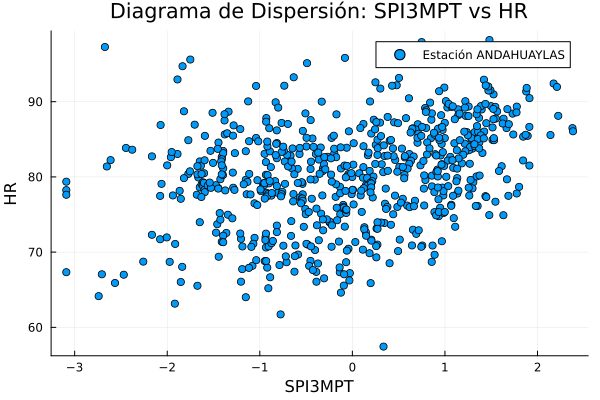
\includegraphics[width=\linewidth]{Capitulos/Scaterplot/ANDAHUAYLAS_SPI3MPT_vs_HR.png}
    \subcaption{SPI3MPT vs HR}
\end{minipage}\hfill
\begin{minipage}{0.33\textwidth}
    \centering
    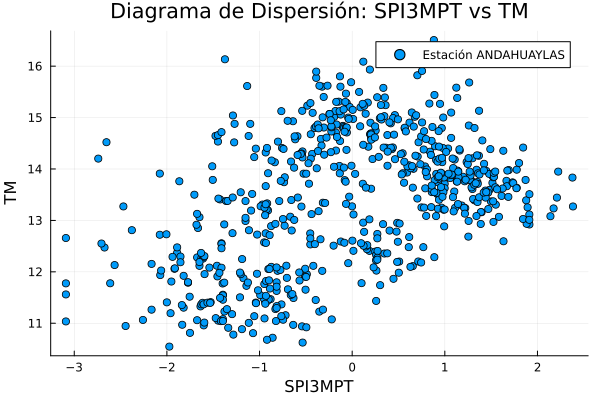
\includegraphics[width=\linewidth]{Capitulos/Scaterplot/ANDAHUAYLAS_SPI3MPT_vs_TM.png}
    \subcaption{SPI3MPT vs TM}
\end{minipage}\hfill
\begin{minipage}{0.33\textwidth}
    \centering
    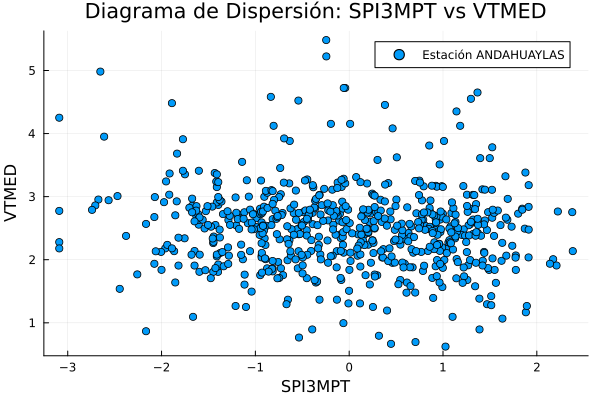
\includegraphics[width=\linewidth]{Capitulos/Scaterplot/ANDAHUAYLAS_SPI3MPT_vs_VTMED.png}
    \subcaption{SPI3MPT vs VTMED}
\end{minipage}

\vspace{0.3cm}  % Espacio entre filas de subgráficas

\begin{minipage}{0.33\textwidth}
    \centering
    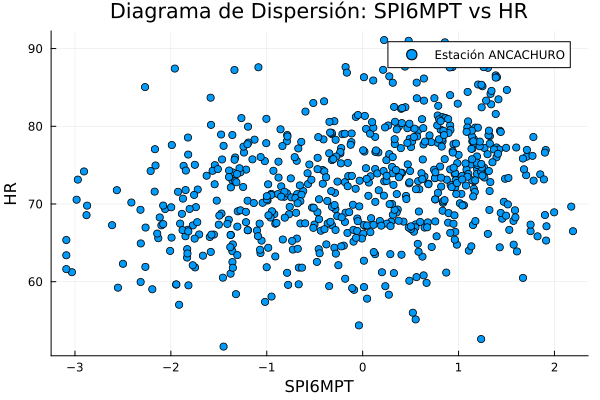
\includegraphics[width=\linewidth]{Capitulos/Scaterplot/ANCACHURO_SPI6MPT_vs_HR.png}
    \subcaption{SPI6MPT vs HR}
\end{minipage}\hfill
\begin{minipage}{0.33\textwidth}
    \centering
    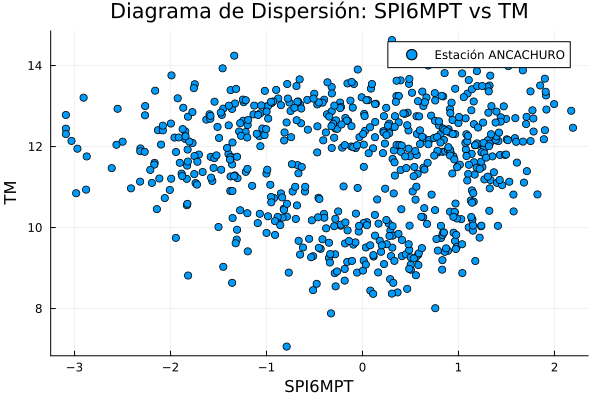
\includegraphics[width=\linewidth]{Capitulos/Scaterplot/ANCACHURO_SPI6MPT_vs_TM.png}
    \subcaption{SPI6MPT vs TM}
\end{minipage}\hfill
\begin{minipage}{0.33\textwidth}
    \centering
    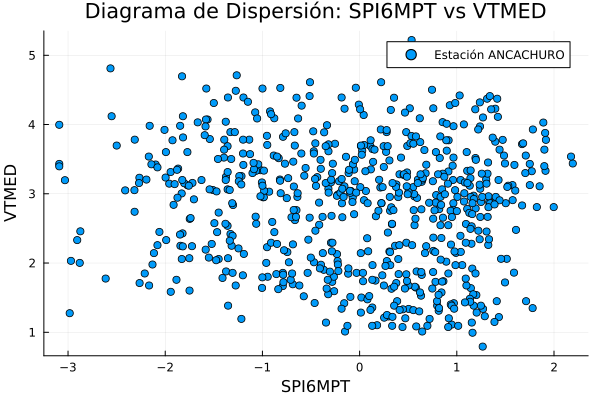
\includegraphics[width=\linewidth]{Capitulos/Scaterplot/ANCACHURO_SPI6MPT_vs_VTMED.png}
    \subcaption{SPI6MPT vs VTMED}
\end{minipage}

\vspace{0.3cm}  % Espacio entre filas de subgráficas

\begin{minipage}{0.33\textwidth}
    \centering
    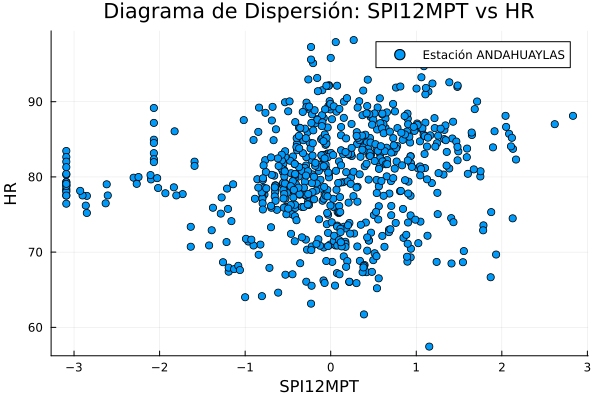
\includegraphics[width=\linewidth]{Capitulos/Scaterplot/ANDAHUAYLAS_SPI12MPT_vs_HR.png}
    \subcaption{SPI12MPT vs HR}
\end{minipage}\hfill
\begin{minipage}{0.33\textwidth}
    \centering
    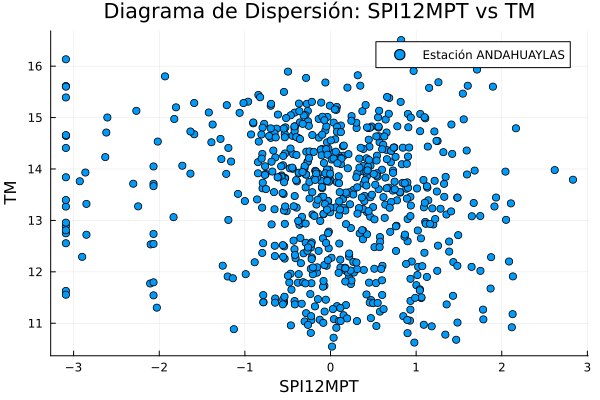
\includegraphics[width=\linewidth]{Capitulos/Scaterplot/ANDAHUAYLAS_SPI12MPT_vs_TM.png}
    \subcaption{SPI12MPT vs TM}
\end{minipage}\hfill
\begin{minipage}{0.33\textwidth}
    \centering
    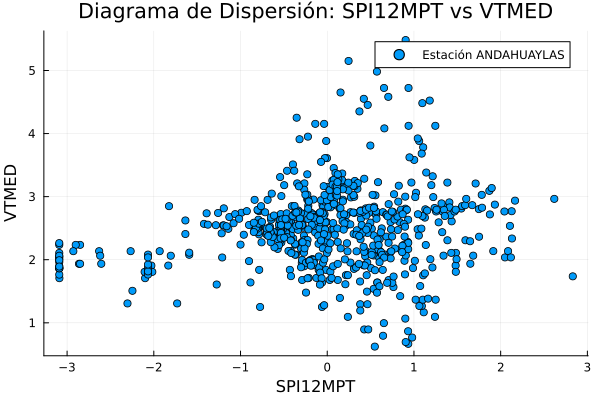
\includegraphics[width=\linewidth]{Capitulos/Scaterplot/ANDAHUAYLAS_SPI12MPT_vs_VTMED.png}
    \subcaption{SPI12MPT vs VTMED}
\end{minipage}
\vspace{0.1em}
\begin{flushleft}
\label{fig:corr_and}
\footnotesize
\justifying
\textbf{\textit{Nota}}: Las combinaciones \textbf{SPI3MPT vs HR} y \textbf{SPI6MPT vs HR} presentan dependencias lineales moderadas, por lo que se recomienda aplicar \textbf{cópulas elípticas} (normal o t de Student). En cambio, las combinaciones \textbf{SPI6MPT vs VTMED} y \textbf{SPI12MPT vs HR} muestran relaciones no lineales, por lo que son más adecuadas para modelarse con \textbf{cópulas arquimedianas} (Clayton, Gumbel o Frank).
\end{flushleft}
\end{figure}






\begin{table}[H]
\centering
\caption{Matrices de Correlación para la Estación Andahuaylas}
\begin{tabular}{lrrrrrrr}
\toprule
\multicolumn{8}{l}{\textbf{Matriz Pearson}} \\
\midrule
Variable & PT & HR & TM & VTMED & SPI3MPT & SPI6MPT & SPI12MPT \\
\midrule
PT       & 1.00 & 0.31 & 0.44 & -0.07 & 0.75 & 0.30 & 0.21 \\
HR       & 0.31 & 1.00 & -0.04 & -0.15 & 0.33 & 0.34 & 0.15 \\
TM       & 0.44 & -0.04 & 1.00 & 0.07 & 0.43 & -0.29 & -0.11 \\
VTMED    & -0.07 & -0.15 & 0.07 & 1.00 & -0.09 & -0.09 & 0.16 \\
SPI3MPT  & 0.75 & 0.33 & 0.43 & -0.09 & 1.00 & 0.61 & 0.23 \\
SPI6MPT  & 0.30 & 0.34 & -0.29 & -0.09 & 0.61 & 1.00 & 0.34 \\
SPI12MPT & 0.21 & 0.15 & -0.11 & 0.16 & 0.23 & 0.34 & 1.00 \\
\midrule
\multicolumn{8}{l}{\textbf{Matriz Spearman}} \\
\midrule
PT       & 1.00 & 0.27 & 0.56 & -0.06 & 0.77 & 0.20 & 0.17 \\
HR       & 0.27 & 1.00 & -0.07 & -0.22 & 0.34 & 0.35 & 0.22 \\
TM       & 0.56 & -0.07 & 1.00 & 0.04 & 0.39 & -0.30 & -0.12 \\
VTMED    & -0.06 & -0.22 & 0.04 & 1.00 & -0.09 & -0.09 & 0.13 \\
SPI3MPT  & 0.77 & 0.34 & 0.39 & -0.09 & 1.00 & 0.64 & 0.21 \\
SPI6MPT  & 0.20 & 0.35 & -0.30 & -0.09 & 0.64 & 1.00 & 0.31 \\
SPI12MPT & 0.17 & 0.22 & -0.12 & 0.13 & 0.21 & 0.31 & 1.00 \\
\midrule
\multicolumn{8}{l}{\textbf{Matriz Kendall}} \\
\midrule
PT       & 0.997 & 0.18 & 0.35 & -0.04 & 0.58 & 0.15 & 0.11 \\
HR       & 0.18 & 0.999 & -0.05 & -0.16 & 0.23 & 0.24 & 0.14 \\
TM       & 0.35 & -0.05 & 0.999 & 0.03 & 0.23 & -0.21 & -0.08 \\
VTMED    & -0.04 & -0.16 & 0.03 & 0.999 & -0.06 & -0.06 & 0.09 \\
SPI3MPT  & 0.58 & 0.23 & 0.23 & -0.06 & 0.999 & 0.47 & 0.14 \\
SPI6MPT  & 0.15 & 0.24 & -0.21 & -0.06 & 0.47 & 0.999 & 0.22 \\
SPI12MPT & 0.11 & 0.14 & -0.08 & 0.09 & 0.14 & 0.22 & 0.999 \\
\midrule
\multicolumn{8}{l}{\textbf{Matriz de Covarianza}} \\
\midrule
PT       & 2450.01 & 104.38 & 27.70 & -2.19 & 41.11 & 15.78 & 10.73 \\
HR       & 104.38 & 44.84 & -0.38 & -0.65 & 2.44 & 2.41 & 1.03 \\
TM       & 27.70 & -0.38 & 1.62 & 0.05 & 0.61 & -0.39 & -0.14 \\
VTMED    & -2.19 & -0.65 & 0.05 & 0.42 & -0.07 & -0.06 & 0.11 \\
SPI3MPT  & 41.11 & 2.44 & 0.61 & -0.07 & 1.23 & 0.72 & 0.25 \\
SPI6MPT  & 15.78 & 2.41 & -0.39 & -0.06 & 0.72 & 1.13 & 0.36 \\
SPI12MPT & 10.73 & 1.03 & -0.14 & 0.11 & 0.25 & 0.36 & 1.02 \\
\bottomrule
\end{tabular}
\end{table}


\begin{table}[htbp]
\centering
\caption{Estadísticas de la Estación \textit{ANCACHURO}}  % Título de la tabla
\resizebox{1\textwidth}{!}{ % Ajuste de la tabla al tamaño deseado
\begin{tabular}{lccccccc}
\hline
\rowcolor{gray!20} \textbf{Statistics} & \textbf{PT} & \textbf{HR} & \textbf{TM} & \textbf{VTMED} & \textbf{SPI3} & \textbf{SPI6} & \textbf{SPI12} \\
\hline
\textit{n} & 648.0 & 648.0 & 648.0 & 648.0 & 648.0 & 648.0 & 648.0 \\
\textit{Minimum} & 0.0 & 51.6447 & 7.06052 & 0.793283 & -3.09023 & -3.09023 & -3.09023 \\
\textit{1st. Quartile} & 6.3 & 67.4579 & 10.3981 & 2.05799 & -1.19127 & -0.91089 & -0.652874 \\
\textit{Median} & 43.15 & 72.7279 & 11.8813 & 2.95505 & 0.0522464 & 0.112471 & 0.0386238 \\
\textit{Mean} & 65.5972 & 72.4477 & 11.5801 & 2.81157 & -0.187156 & -0.0528842 & -0.00152609 \\
\textit{3rd. Quartile} & 113.225 & 77.2875 & 12.683 & 3.43961 & 0.926963 & 0.872971 & 0.605086 \\
\textit{Maximum} & 296.7 & 91.0981 & 14.6287 & 5.21975 & 2.16014 & 2.19327 & 2.60037 \\
\textit{Rank} & 296.7 & 39.4535 & 7.56822 & 4.42647 & 5.25037 & 5.28351 & 5.6906 \\
\textit{Interquartile Rank} & 106.925 & 9.82963 & 2.28489 & 1.38162 & 2.11823 & 1.78386 & 1.25796 \\
\textit{Variance} & 4478.19 & 47.7106 & 1.98259 & 0.808566 & 1.65859 & 1.29194 & 1.02633 \\
\textit{Standard Deviation} & 66.9193 & 6.90729 & 1.40804 & 0.899203 & 1.28786 & 1.13664 & 1.01308 \\
\textit{Variation Coeff.} & 1.02015 & 0.0953417 & 0.121591 & 0.319823 & -6.88121 & -21.4929 & -663.839 \\
\textit{Skewness} & 0.915823 & 0.0611358 & -0.466041 & -0.132546 & -0.40047 & -0.428827 & -0.365281 \\
\textit{Kurtosis} & 0.00825298 & -0.150893 & -0.663921 & -0.817877 & -0.831534 & -0.617489 & 0.527641 \\
\hline
\end{tabular}
}
\end{table}



\begin{figure}[htbp]
\centering
\caption{Gráficas de dispersión para la Estación \textit{ANCACHURO}}
\begin{minipage}{0.32\textwidth}
    \centering
    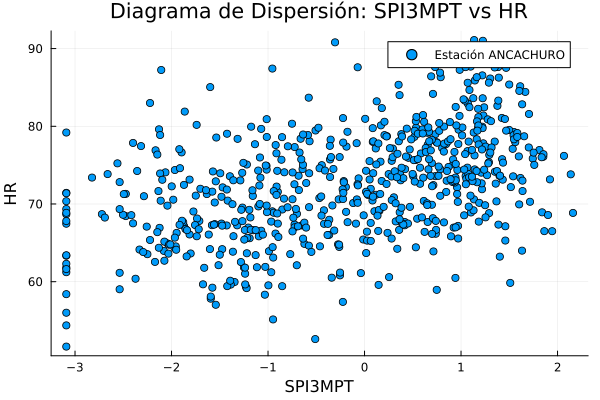
\includegraphics[width=\linewidth]{Capitulos/Scaterplot/ANCACHURO_SPI3MPT_vs_HR.png}
    \subcaption{SPI3MPT vs HR}
\end{minipage}\hfill
\begin{minipage}{0.32\textwidth}
    \centering
    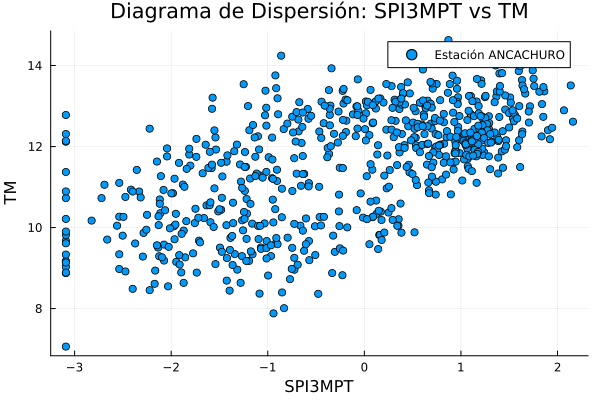
\includegraphics[width=\linewidth]{Capitulos/Scaterplot/ANCACHURO_SPI3MPT_vs_TM.png}
    \subcaption{SPI3MPT vs TM}
\end{minipage}\hfill
\begin{minipage}{0.32\textwidth}
    \centering
    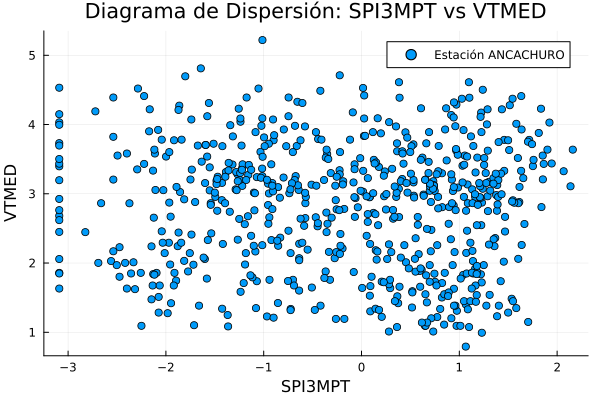
\includegraphics[width=\linewidth]{Capitulos/Scaterplot/ANCACHURO_SPI3MPT_vs_VTMED.png}
    \subcaption{SPI3MPT vs VTMED}
\end{minipage}

\vspace{0.5cm}  % Espacio entre filas de subgráficas

\begin{minipage}{0.32\textwidth}
    \centering
    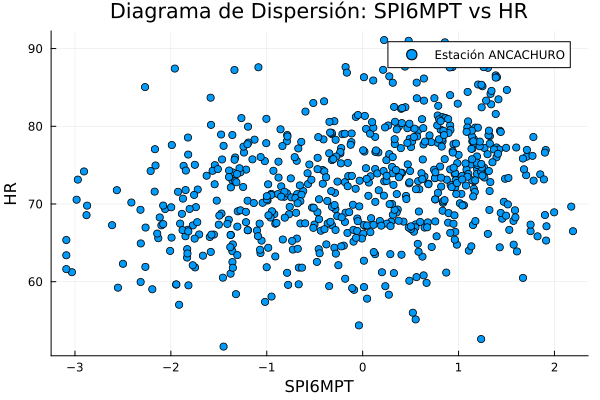
\includegraphics[width=\linewidth]{Capitulos/Scaterplot/ANCACHURO_SPI6MPT_vs_HR.png}
    \subcaption{SPI6MPT vs HR}
\end{minipage}\hfill
\begin{minipage}{0.32\textwidth}
    \centering
    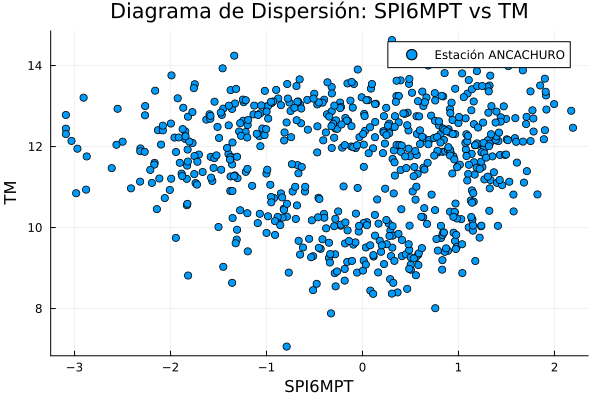
\includegraphics[width=\linewidth]{Capitulos/Scaterplot/ANCACHURO_SPI6MPT_vs_TM.png}
    \subcaption{SPI6MPT vs TM}
\end{minipage}\hfill
\begin{minipage}{0.32\textwidth}
    \centering
    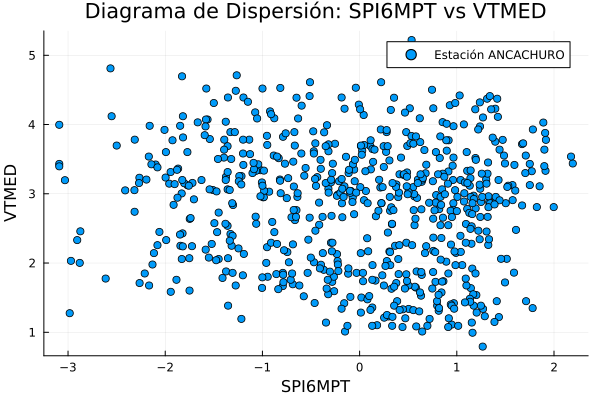
\includegraphics[width=\linewidth]{Capitulos/Scaterplot/ANCACHURO_SPI6MPT_vs_VTMED.png}
    \subcaption{SPI6MPT vs VTMED}
\end{minipage}

\vspace{0.5cm}  % Espacio entre filas de subgráficas

\begin{minipage}{0.32\textwidth}
    \centering
    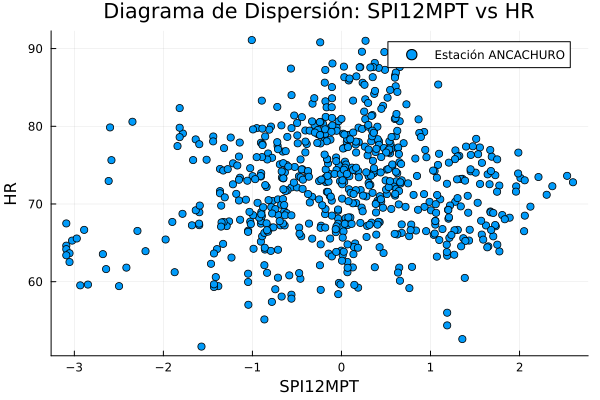
\includegraphics[width=\linewidth]{Capitulos/Scaterplot/ANCACHURO_SPI12MPT_vs_HR.png}
    \subcaption{SPI12MPT vs HR}
\end{minipage}\hfill
\begin{minipage}{0.32\textwidth}
    \centering
    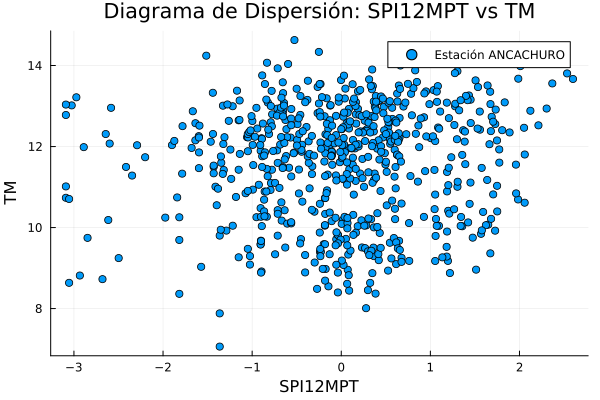
\includegraphics[width=\linewidth]{Capitulos/Scaterplot/ANCACHURO_SPI12MPT_vs_TM.png}
    \subcaption{SPI12MPT vs TM}
\end{minipage}\hfill
\begin{minipage}{0.32\textwidth}
    \centering
    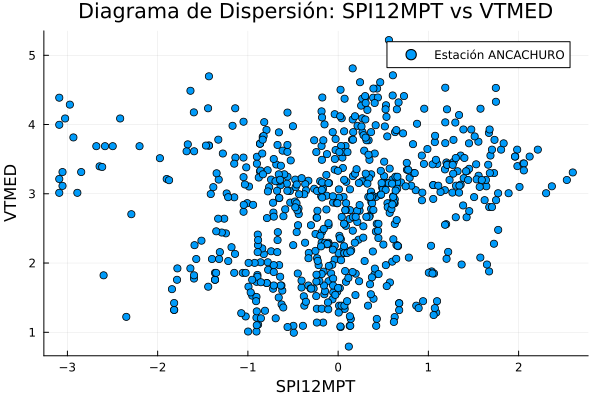
\includegraphics[width=\linewidth]{Capitulos/Scaterplot/ANCACHURO_SPI12MPT_vs_VTMED.png}
    \subcaption{SPI12MPT vs VTMED}
\end{minipage}

\end{figure}



Los resultados obtenidos de las estadísticas descriptivas y las matrices de correlación para la estación \textit{Ancachuro} permiten una interpretación detallada de las relaciones entre las variables meteorológicas y los índices de precipitación estandarizada. En la primera tabla , se presentan diversas estadísticas de resumen para las variables PT (Temperatura), HR (Humedad Relativa), TM (Temperatura máxima), VTMED (Velocidad media del viento), SPI3MPT (Índice de precipitación estandarizada a 3 meses), SPI6MPT (Índice de precipitación estandarizada a 6 meses) y SPI12MPT (Índice de precipitación estandarizada a 12 meses). Las estadísticas incluyen la media, mediana, cuartiles, varianza, desviación estándar, coeficiente de variación, asimetría, y curtosis, entre otros. Los valores de estas estadísticas proporcionan una visión general de la distribución de cada variable.

Por otro lado, en la segunda tabla (Tabla 2) se presentan las matrices de correlación bivariada para las mismas variables. Se calcula la correlación de Pearson, Spearman y Kendall, lo que permite identificar la fuerza y naturaleza de las dependencias entre las variables. En particular, se observa que \textit{HR} (Humedad Relativa) y \textit{SPI3MPT} (Índice de precipitación a 3 meses) presentan una alta correlación positiva, lo que sugiere una fuerte dependencia lineal entre ambas variables, que podría modelarse utilizando cópulas elípticas. Por otro lado, las variables como \textit{VTMED} (Velocidad media del viento) y \textit{SPI3MPT} tienen correlaciones más débiles, lo que sugiere que una cópula más simple o incluso independiente podría ser apropiada para modelar la relación entre ellas.

En cuanto a las dependencias no lineales, se observa que algunas variables presentan correlaciones significativas en las medidas de Spearman y Kendall, lo que sugiere que para estas relaciones podría ser más adecuado el uso de cópulas arquimedianas, como la cópula de Clayton o Gumbel, que pueden capturar dependencias no lineales y asimétricas.

En resumen, los resultados obtenidos de las estadísticas descriptivas y las correlaciones bivariadas sugieren que, para las variables fuertemente correlacionadas, como \textit{HR} y \textit{SPI3MPT}, se podrían aplicar cópulas elípticas, mientras que para las relaciones no lineales, como las que involucran \textit{VTMED} y las variables de precipitación, las cópulas arquimedianas serían más apropiadas. Esto proporciona una base sólida para el análisis posterior mediante cópulas bivariadas, permitiendo modelar adecuadamente las dependencias entre las variables meteorológicas en la estación \textit{Ancachuro}.




\begin{table}[ht]
\centering
\caption{Matrices de Correlación para la Estación Ancachuro}
\begin{tabular}{lrrrrrrr}
\toprule
\multicolumn{8}{l}{\textbf{Matriz Pearson}} \\
\midrule
Variable & PT & HR & TM & VTMED & SPI3MPT & SPI6MPT & SPI12MPT \\
\midrule
PT       & 1.00 & 0.40 & 0.65 & 0.03 & 0.75 & 0.32 & 0.18 \\
HR       & 0.40 & 1.00 & 0.21 & -0.16 & 0.46 & 0.30 & 0.10 \\
TM       & 0.65 & 0.21 & 1.00 & 0.10 & 0.61 & -0.01 & 0.09 \\
VTMED    & 0.03 & -0.16 & 0.10 & 1.00 & -0.04 & -0.09 & 0.15 \\
SPI3MPT  & 0.75 & 0.46 & 0.61 & -0.04 & 1.00 & 0.64 & 0.19 \\
SPI6MPT  & 0.32 & 0.30 & -0.01 & -0.09 & 0.64 & 1.00 & 0.30 \\
SPI12MPT & 0.18 & 0.10 & 0.09 & 0.15 & 0.19 & 0.30 & 1.00 \\
\midrule
\multicolumn{8}{l}{\textbf{Matriz Spearman}} \\
\midrule
PT       & 1.00 & 0.42 & 0.73 & 0.03 & 0.79 & 0.25 & 0.16 \\
HR       & 0.42 & 1.00 & 0.21 & -0.19 & 0.47 & 0.31 & 0.07 \\
TM       & 0.73 & 0.21 & 1.00 & 0.11 & 0.60 & 0.01 & 0.09 \\
VTMED    & 0.03 & -0.19 & 0.11 & 1.00 & -0.03 & -0.09 & 0.20 \\
SPI3MPT  & 0.79 & 0.47 & 0.60 & -0.03 & 1.00 & 0.67 & 0.20 \\
SPI6MPT  & 0.25 & 0.31 & 0.01 & -0.09 & 0.67 & 1.00 & 0.30 \\
SPI12MPT & 0.16 & 0.07 & 0.09 & 0.20 & 0.20 & 0.30 & 1.00 \\
\midrule
\multicolumn{8}{l}{\textbf{Matriz Kendall}} \\
\midrule
PT       & 0.98 & 0.29 & 0.51 & 0.02 & 0.60 & 0.18 & 0.11 \\
HR       & 0.29 & 1.00 & 0.13 & -0.13 & 0.32 & 0.21 & 0.05 \\
TM       & 0.51 & 0.13 & 1.00 & 0.07 & 0.41 & 0.01 & 0.06 \\
VTMED    & 0.02 & -0.13 & 0.07 & 1.00 & -0.02 & -0.06 & 0.14 \\
SPI3MPT  & 0.60 & 0.32 & 0.41 & -0.02 & 1.00 & 0.49 & 0.14 \\
SPI6MPT  & 0.18 & 0.21 & 0.01 & -0.06 & 0.49 & 1.00 & 0.21 \\
SPI12MPT & 0.11 & 0.05 & 0.06 & 0.14 & 0.14 & 0.21 & 1.00 \\
\midrule
\multicolumn{8}{l}{\textbf{Matriz de Covarianza}} \\
\midrule
PT       & 4478.19 & 182.62 & 61.17 & 2.09 & 64.65 & 24.36 & 12.44 \\
HR       & 182.62 & 47.71 & 2.06 & -1.02 & 4.09 & 2.37 & 0.71 \\
TM       & 61.17 & 2.06 & 1.98 & 0.13 & 1.11 & -0.01 & 0.12 \\
VTMED    & 2.09 & -1.02 & 0.13 & 0.81 & -0.04 & -0.10 & 0.14 \\
SPI3MPT  & 64.65 & 4.09 & 1.11 & -0.04 & 1.66 & 0.94 & 0.24 \\
SPI6MPT  & 24.36 & 2.37 & -0.01 & -0.10 & 0.94 & 1.29 & 0.35 \\
SPI12MPT & 12.44 & 0.71 & 0.12 & 0.14 & 0.24 & 0.35 & 1.03 \\
\bottomrule
\end{tabular}
\end{table}




\begin{table}[htbp]
\centering
\caption{Estadísticas de la Estación \textit{CAYRA}}  % Título de la tabla
\resizebox{1\textwidth}{!}{ % Ajuste de la tabla al tamaño deseado
\begin{tabular}{lccccccc}
\hline
\rowcolor{gray!20} \textbf{Statistics} & \textbf{PT} & \textbf{HR} & \textbf{TM} & \textbf{VTMED} & \textbf{SPI3} & \textbf{SPI6} & \textbf{SPI12} \\
\hline
\textit{n} & 648.0 & 648.0 & 648.0 & 648.0 & 648.0 & 648.0 & 648.0 \\
\textit{Minimum} & 0.0 & 63.05 & 8.59786 & 0.0 & -3.09023 & -2.80259 & -3.09023 \\
\textit{1st. Quartile} & 5.9 & 68.81 & 11.1943 & 1.0104 & -1.16446 & -0.978838 & -0.682226 \\
\textit{Median} & 40.35 & 71.39 & 12.6816 & 1.35397 & 0.0504715 & 0.155268 & 0.00707127 \\
\textit{Mean} & 57.1098 & 72.0591 & 12.3963 & 1.44522 & -0.139489 & -0.0534459 & 0.000156151 \\
\textit{3rd. Quartile} & 101.95 & 75.56 & 13.5351 & 1.76352 & 0.988857 & 0.90486 & 0.67652 \\
\textit{Maximum} & 268.5 & 77.61 & 15.7556 & 4.07704 & 2.01945 & 2.06429 & 2.50055 \\
\textit{Rank} & 268.5 & 14.56 & 7.15779 & 4.07704 & 5.10969 & 4.86687 & 5.59079 \\
\textit{Interquartile Rank} & 96.05 & 6.75 & 2.34078 & 0.753123 & 2.15332 & 1.8837 & 1.35875 \\
\textit{Variance} & 3241.52 & 18.3112 & 2.37034 & 0.363134 & 1.55681 & 1.30031 & 0.993172 \\
\textit{Standard Deviation} & 56.9344 & 4.27915 & 1.53959 & 0.602606 & 1.24772 & 1.14031 & 0.99658 \\
\textit{Variation Coeff.} & 0.996927 & 0.059384 & 0.124197 & 0.416966 & -8.94499 & -21.3358 & 6382.18 \\
\textit{Skewness} & 0.847616 & -0.242397 & -0.380765 & 0.858175 & -0.326602 & -0.403467 & -0.131677 \\
\textit{Kurtosis} & -0.194441 & -0.940006 & -0.812793 & 1.07509 & -1.03735 & -0.941653 & 0.0326297 \\
\hline
\end{tabular}
}
\end{table}



\begin{figure}[htbp]
\centering
\caption{Gráficas de dispersión para la Estación \textit{CAYRA}}
\begin{minipage}{0.32\textwidth}
    \centering
    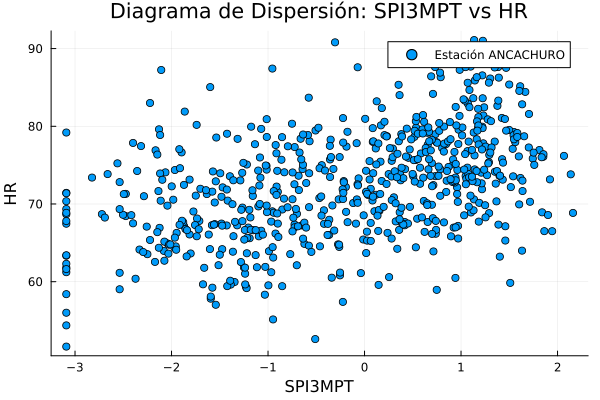
\includegraphics[width=\linewidth]{Capitulos/Scaterplot/ANCACHURO_SPI3MPT_vs_HR.png}
    \subcaption{SPI3MPT vs HR}
\end{minipage}\hfill
\begin{minipage}{0.32\textwidth}
    \centering
    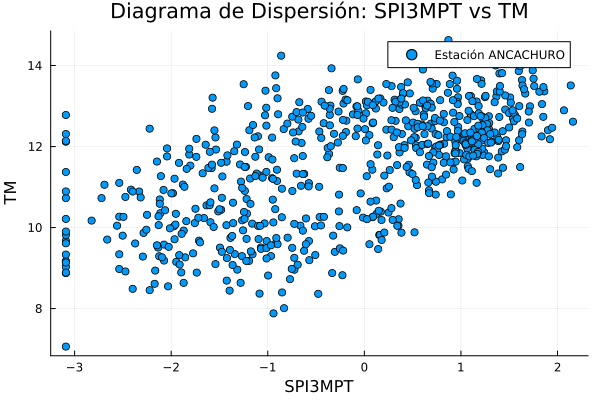
\includegraphics[width=\linewidth]{Capitulos/Scaterplot/ANCACHURO_SPI3MPT_vs_TM.png}
    \subcaption{SPI3MPT vs TM}
\end{minipage}\hfill
\begin{minipage}{0.32\textwidth}
    \centering
    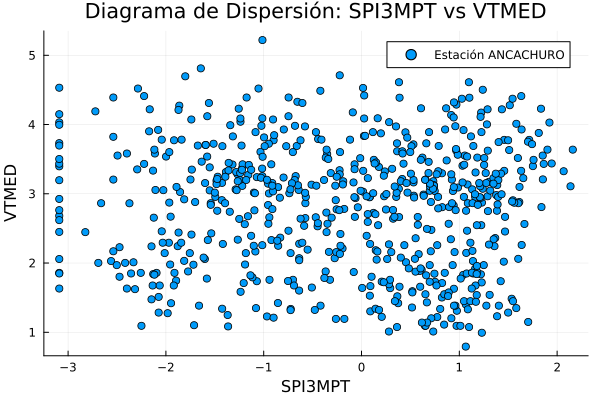
\includegraphics[width=\linewidth]{Capitulos/Scaterplot/ANCACHURO_SPI3MPT_vs_VTMED.png}
    \subcaption{SPI3MPT vs VTMED}
\end{minipage}

\vspace{0.5cm}  % Espacio entre filas de subgráficas

\begin{minipage}{0.32\textwidth}
    \centering
    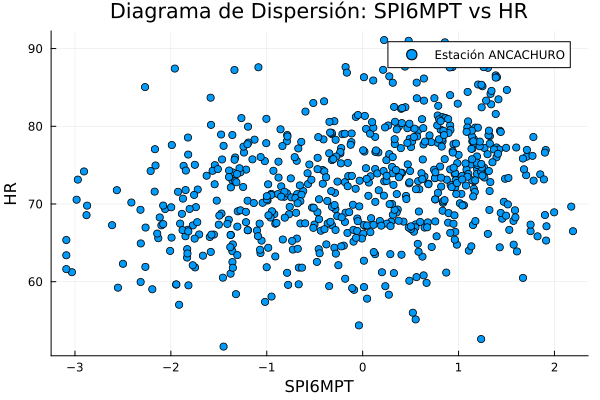
\includegraphics[width=\linewidth]{Capitulos/Scaterplot/ANCACHURO_SPI6MPT_vs_HR.png}
    \subcaption{SPI6MPT vs HR}
\end{minipage}\hfill
\begin{minipage}{0.32\textwidth}
    \centering
    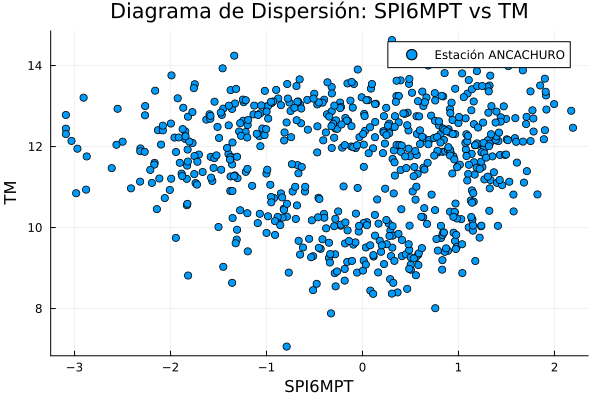
\includegraphics[width=\linewidth]{Capitulos/Scaterplot/ANCACHURO_SPI6MPT_vs_TM.png}
    \subcaption{SPI6MPT vs TM}
\end{minipage}\hfill
\begin{minipage}{0.32\textwidth}
    \centering
    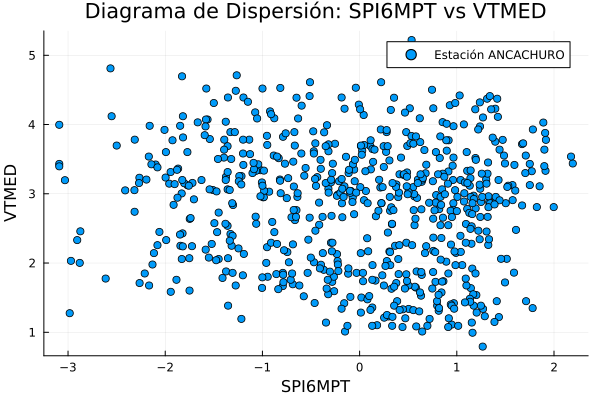
\includegraphics[width=\linewidth]{Capitulos/Scaterplot/ANCACHURO_SPI6MPT_vs_VTMED.png}
    \subcaption{SPI6MPT vs VTMED}
\end{minipage}

\vspace{0.5cm}  % Espacio entre filas de subgráficas

\begin{minipage}{0.32\textwidth}
    \centering
    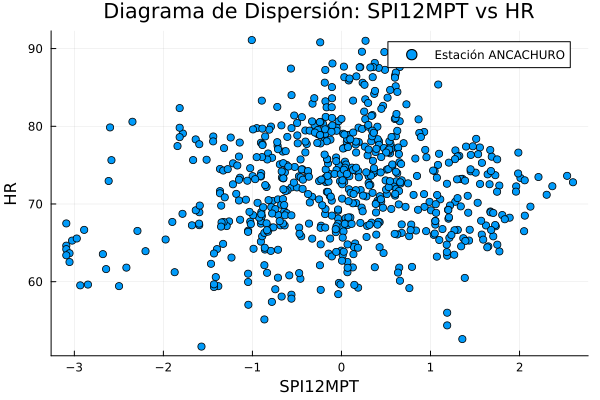
\includegraphics[width=\linewidth]{Capitulos/Scaterplot/ANCACHURO_SPI12MPT_vs_HR.png}
    \subcaption{SPI12MPT vs HR}
\end{minipage}\hfill
\begin{minipage}{0.32\textwidth}
    \centering
    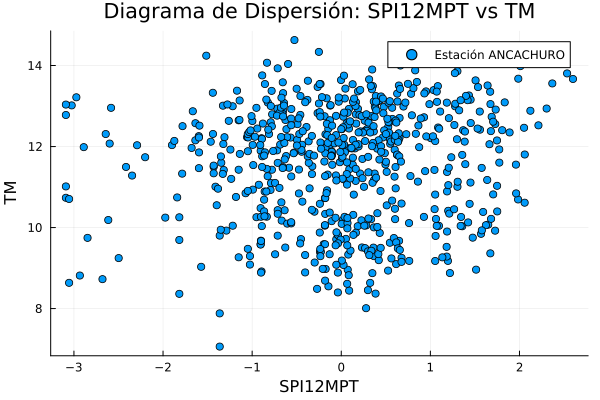
\includegraphics[width=\linewidth]{Capitulos/Scaterplot/ANCACHURO_SPI12MPT_vs_TM.png}
    \subcaption{SPI12MPT vs TM}
\end{minipage}\hfill
\begin{minipage}{0.32\textwidth}
    \centering
    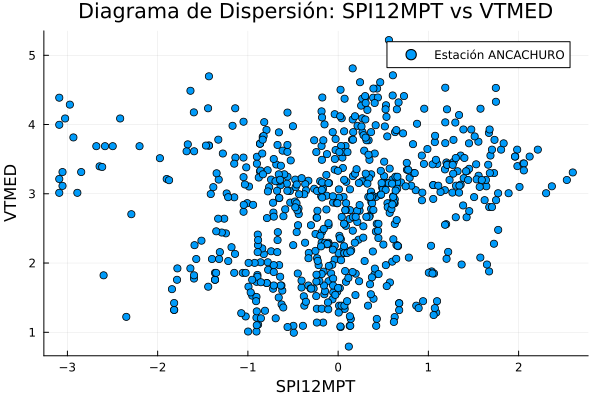
\includegraphics[width=\linewidth]{Capitulos/Scaterplot/ANCACHURO_SPI12MPT_vs_VTMED.png}
    \subcaption{SPI12MPT vs VTMED}
\end{minipage}

\end{figure}


Los resultados obtenidos de las estadísticas descriptivas y las matrices de correlación para la estación \textit{Cayra} proporcionan información útil para el análisis de las relaciones entre las variables meteorológicas y los índices de precipitación estandarizada. En la primera tabla (Tabla 1), se presentan diversas estadísticas de resumen, tales como la media, mediana, cuartiles, varianza, desviación estándar, coeficiente de variación, asimetría y curtosis, para las variables PT (Temperatura), HR (Humedad Relativa), TM (Temperatura máxima), VTMED (Velocidad media del viento), SPI3MPT (Índice de precipitación estandarizada a 3 meses), SPI6MPT (Índice de precipitación estandarizada a 6 meses) y SPI12MPT (Índice de precipitación estandarizada a 12 meses). Estos resultados indican que las variables de temperatura (\textit{PT}, \textit{TM}) y los índices de precipitación presentan una variabilidad considerable, mientras que la humedad relativa (\textit{HR}) y la velocidad del viento (\textit{VTMED}) tienen una mayor estabilidad.

Por otro lado, la segunda tabla (Tabla 2) muestra las matrices de correlación bivariada para las mismas variables, calculadas mediante los coeficientes de correlación de Pearson, Spearman y Kendall. Se observa que la correlación entre \textit{HR} (Humedad Relativa) y \textit{SPI3MPT} (Índice de precipitación estandarizada a 3 meses) es moderadamente fuerte (0.75 en Pearson), lo que sugiere que la humedad relativa y la precipitación a 3 meses están fuertemente relacionadas. También se observa que \textit{VTMED} (Velocidad media del viento) tiene una correlación débil y negativa con algunas de las variables, lo que podría indicar que su relación con las precipitaciones y la humedad es más compleja.

En cuanto a las dependencias no lineales, las matrices de Spearman y Kendall muestran que algunas relaciones entre las variables son asimétricas o no lineales. Esto sugiere que, para modelar las dependencias entre ciertas combinaciones de variables, como entre \textit{SPI6MPT} y \textit{SPI12MPT}, se podrían emplear cópulas arquimedianas, que son capaces de capturar dependencias no lineales. Por otro lado, las correlaciones lineales más fuertes, como la de \textit{HR} y \textit{SPI3MPT}, podrían ser mejor modeladas utilizando cópulas elípticas, como la cópula normal, que es adecuada para relaciones lineales.

En resumen, los resultados obtenidos de las estadísticas descriptivas y las correlaciones bivariadas sugieren que, dependiendo de la intensidad y la naturaleza de las dependencias observadas, se podrían aplicar cópulas elípticas y arquimedianas. Esto proporcionará una base sólida para el análisis posterior de las dependencias bivariadas entre las variables meteorológicas y los índices de precipitación en la estación \textit{Cayra}.


\begin{table}[ht]
\centering
\caption{Matrices de Correlación para la Estación Cayra}
\begin{tabular}{lrrrrrrr}
\toprule
\multicolumn{8}{l}{\textbf{Matriz Pearson}} \\
\midrule
Variable & PT & HR & TM & VTMED & SPI3MPT & SPI6MPT & SPI12MPT \\
\midrule
PT       & 1.00 & 0.08 & 0.55 & -0.15 & 0.77 & 0.30 & 0.13 \\
HR       & 0.08 & 1.00 & 0.00 & -0.12 & 0.16 & 0.21 & 0.00 \\
TM       & 0.55 & 0.00 & 1.00 & 0.26 & 0.44 & -0.29 & -0.05 \\
VTMED    & -0.15 & -0.12 & 0.26 & 1.00 & -0.33 & -0.61 & -0.02 \\
SPI3MPT  & 0.77 & 0.16 & 0.44 & -0.33 & 1.00 & 0.63 & 0.13 \\
SPI6MPT  & 0.30 & 0.21 & -0.29 & -0.61 & 0.63 & 1.00 & 0.21 \\
SPI12MPT & 0.13 & 0.00 & -0.05 & -0.02 & 0.13 & 0.21 & 1.00 \\
\midrule
\multicolumn{8}{l}{\textbf{Matriz Spearman}} \\
\midrule
PT       & 1.00 & 0.08 & 0.64 & -0.07 & 0.81 & 0.23 & 0.11 \\
HR       & 0.08 & 1.00 & 0.00 & -0.13 & 0.18 & 0.22 & 0.04 \\
TM       & 0.64 & 0.00 & 1.00 & 0.25 & 0.39 & -0.28 & -0.07 \\
VTMED    & -0.07 & -0.13 & 0.25 & 1.00 & -0.35 & -0.60 & -0.04 \\
SPI3MPT  & 0.81 & 0.18 & 0.39 & -0.35 & 1.00 & 0.67 & 0.15 \\
SPI6MPT  & 0.23 & 0.22 & -0.28 & -0.60 & 0.67 & 1.00 & 0.23 \\
SPI12MPT & 0.11 & 0.04 & -0.07 & -0.04 & 0.15 & 0.23 & 1.00 \\
\midrule
\multicolumn{8}{l}{\textbf{Matriz Kendall}} \\
\midrule
PT       & 0.99 & 0.06 & 0.43 & -0.05 & 0.61 & 0.16 & 0.08 \\
HR       & 0.06 & 0.88 & 0.00 & -0.09 & 0.12 & 0.15 & 0.02 \\
TM       & 0.43 & 0.00 & 1.00 & 0.17 & 0.24 & -0.18 & -0.05 \\
VTMED    & -0.05 & -0.09 & 0.17 & 1.00 & -0.23 & -0.42 & -0.02 \\
SPI3MPT  & 0.61 & 0.12 & 0.24 & -0.23 & 1.00 & 0.48 & 0.10 \\
SPI6MPT  & 0.16 & 0.15 & -0.18 & -0.42 & 0.48 & 1.00 & 0.17 \\
SPI12MPT & 0.08 & 0.02 & -0.05 & -0.02 & 0.10 & 0.17 & 1.00 \\
\midrule
\multicolumn{8}{l}{\textbf{Matriz de Covarianza}} \\
\midrule
PT       & 3241.52 & 18.89 & 47.87 & -5.11 & 54.49 & 19.22 & 7.56 \\
HR       & 18.89 & 18.31 & 0.02 & -0.32 & 0.88 & 1.01 & 0.00 \\
TM       & 47.87 & 0.02 & 2.37 & 0.24 & 0.84 & -0.50 & -0.08 \\
VTMED    & -5.11 & -0.32 & 0.24 & 0.36 & -0.25 & -0.42 & -0.01 \\
SPI3MPT  & 54.49 & 0.88 & 0.84 & -0.25 & 1.56 & 0.90 & 0.16 \\
SPI6MPT  & 19.22 & 1.01 & -0.50 & -0.42 & 0.90 & 1.30 & 0.24 \\
SPI12MPT & 7.56 & 0.00 & -0.08 & -0.01 & 0.16 & 0.24 & 0.99 \\
\bottomrule
\end{tabular}
\end{table}


\begin{table}[htbp]
\centering
\caption{Estadísticas de la Estación \textit{SICUANI}}  % Título de la tabla
\resizebox{1\textwidth}{!}{ % Ajuste de la tabla al tamaño deseado
\begin{tabular}{lccccccc}
\hline
\rowcolor{gray!20} \textbf{Statistics} & \textbf{PT} & \textbf{HR} & \textbf{TM} & \textbf{VTMED} & \textbf{SPI3} & \textbf{SPI6} & \textbf{SPI12} \\
\hline
\textit{n} & 648.0 & 648.0 & 648.0 & 648.0 & 648.0 & 648.0 & 648.0 \\
\textit{Minimum} & 0.0 & 43.5111 & 7.14 & 0.0 & -3.09023 & -3.09023 & -3.09023 \\
\textit{1st. Quartile} & 6.57073 & 57.8864 & 10.4075 & 1.35756 & -1.15818 & -0.930762 & -0.485108 \\
\textit{Median} & 45.3088 & 64.9032 & 11.925 & 1.82063 & 0.0728518 & 0.164545 & -0.0789637 \\
\textit{Mean} & 60.4047 & 64.1581 & 11.5917 & 2.02239 & -0.177522 & -0.0525821 & 0.00237571 \\
\textit{3rd. Quartile} & 108.3 & 71.2594 & 12.7457 & 2.36073 & 0.992302 & 0.934639 & 0.562663 \\
\textit{Maximum} & 259.5 & 81.4872 & 15.3 & 17.1432 & 2.01184 & 1.90971 & 3.09023 \\
\textit{Rank} & 259.5 & 37.9762 & 8.16 & 17.1432 & 5.10207 & 4.99994 & 6.18046 \\
\textit{Interquartile Rank} & 101.729 & 13.373 & 2.33815 & 1.00316 & 2.15049 & 1.8654 & 1.04777 \\
\textit{Variance} & 3368.68 & 66.5806 & 2.60445 & 1.87521 & 1.71938 & 1.31414 & 0.969949 \\
\textit{Standard Deviation} & 58.0404 & 8.15969 & 1.61383 & 1.36938 & 1.31125 & 1.14636 & 0.98486 \\
\textit{Variation Coeff.} & 0.960858 & 0.127181 & 0.139223 & 0.677112 & -7.38641 & -21.8013 & 414.554 \\
\textit{Skewness} & 0.704625 & -0.306555 & -0.464899 & 5.20471 & -0.453777 & -0.462943 & -0.0260507 \\
\textit{Kurtosis} & -0.568756 & -0.940006 & -0.453473 & 42.178 & -0.921569 & -0.861539 & 1.23526 \\
\hline
\end{tabular}
}
\end{table}


\begin{figure}[htbp]
\centering
\caption{Gráficas de dispersión para la Estación \textit{SICUANI}}
\begin{minipage}{0.32\textwidth}
    \centering
    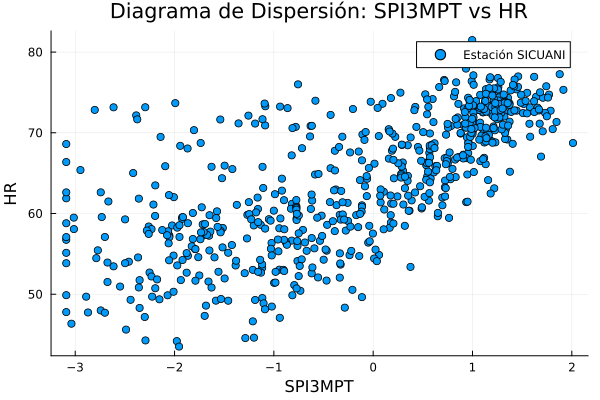
\includegraphics[width=\linewidth]{Capitulos/Scaterplot/SICUANI_SPI3MPT_vs_HR.png}
    \subcaption{SPI3MPT vs HR}
\end{minipage}\hfill
\begin{minipage}{0.32\textwidth}
    \centering
    \includegraphics[width=\linewidth]{Capitulos/Scaterplot/SICUANI_SPI3MPT_vs_TM.png}
    \subcaption{SPI3MPT vs TM}
\end{minipage}\hfill
\begin{minipage}{0.32\textwidth}
    \centering
    \includegraphics[width=\linewidth]{Capitulos/Scaterplot/SICUANI_SPI3MPT_vs_VTMED.png}
    \subcaption{SPI3MPT vs VTMED}
\end{minipage}

\vspace{0.5cm}  % Espacio entre filas de subgráficas

\begin{minipage}{0.32\textwidth}
    \centering
    \includegraphics[width=\linewidth]{Capitulos/Scaterplot/SICUANI_SPI6MPT_vs_HR.png}
    \subcaption{SPI6MPT vs HR}
\end{minipage}\hfill
\begin{minipage}{0.32\textwidth}
    \centering
    \includegraphics[width=\linewidth]{Capitulos/Scaterplot/SICUANI_SPI6MPT_vs_TM.png}
    \subcaption{SPI6MPT vs TM}
\end{minipage}\hfill
\begin{minipage}{0.32\textwidth}
    \centering
    \includegraphics[width=\linewidth]{Capitulos/Scaterplot/SICUANI_SPI6MPT_vs_VTMED.png}
    \subcaption{SPI6MPT vs VTMED}
\end{minipage}

\vspace{0.5cm}  % Espacio entre filas de subgráficas

\begin{minipage}{0.32\textwidth}
    \centering
    \includegraphics[width=\linewidth]{Capitulos/Scaterplot/SICUANI_SPI12MPT_vs_HR.png}
    \subcaption{SPI12MPT vs HR}
\end{minipage}\hfill
\begin{minipage}{0.32\textwidth}
    \centering
    \includegraphics[width=\linewidth]{Capitulos/Scaterplot/SICUANI_SPI12MPT_vs_TM.png}
    \subcaption{SPI12MPT vs TM}
\end{minipage}\hfill
\begin{minipage}{0.32\textwidth}
    \centering
    \includegraphics[width=\linewidth]{Capitulos/Scaterplot/SICUANI_SPI12MPT_vs_VTMED.png}
    \subcaption{SPI12MPT vs VTMED}
\end{minipage}

\end{figure}


Los resultados obtenidos de las estadísticas descriptivas y las matrices de correlación para la estación \textit{Sicuani} ofrecen una visión clara sobre las relaciones entre las variables meteorológicas y los índices de precipitación estandarizada. En la primera tabla (Tabla 1), se presentan las estadísticas de resumen, como la media, mediana, cuartiles, desviación estándar, coeficiente de variación, asimetría y curtosis para las variables PT (Temperatura), HR (Humedad Relativa), TM (Temperatura máxima), VTMED (Velocidad media del viento), SPI3MPT (Índice de precipitación estandarizada a 3 meses), SPI6MPT (Índice de precipitación estandarizada a 6 meses), y SPI12MPT (Índice de precipitación estandarizada a 12 meses). Los valores de estas estadísticas sugieren que las variables de temperatura (\textit{PT}, \textit{TM}) y los índices de precipitación tienen una alta variabilidad, mientras que la humedad relativa (\textit{HR}) y la velocidad del viento (\textit{VTMED}) muestran una mayor estabilidad.

En la segunda tabla (Tabla 2), se muestran las matrices de correlación bivariada entre las variables, calculadas mediante los coeficientes de correlación de Pearson, Spearman y Kendall. Se observa que la humedad relativa (\textit{HR}) y el índice de precipitación estandarizado a 3 meses (\textit{SPI3MPT}) tienen una correlación significativa, tanto en Pearson como en Spearman, lo que sugiere que ambas variables están fuertemente relacionadas y que una cópula elíptica, como la cópula normal, podría ser adecuada para modelar esta dependencia lineal. Por otro lado, las variables como la velocidad media del viento (\textit{VTMED}) y el índice de precipitación estandarizado presentan correlaciones débiles, lo que podría indicar que estas relaciones no son lineales y que se podría considerar el uso de cópulas arquimedianas, como la cópula de Clayton o Gumbel, que pueden capturar dependencias no lineales.

Adicionalmente, la matriz de Kendall muestra que existen algunas dependencias no lineales entre variables, como en el caso de \textit{SPI6MPT} y \textit{SPI12MPT}, lo que refuerza la recomendación de utilizar cópulas arquimedianas para estas combinaciones de variables. En resumen, los resultados obtenidos sugieren que, para las relaciones lineales, como la de \textit{HR} y \textit{SPI3MPT}, se deberían aplicar cópulas elípticas, mientras que para las dependencias no lineales, como las que involucran \textit{SPI6MPT} y \textit{SPI12MPT}, las cópulas arquimedianas serían más apropiadas. Esto proporciona una base sólida para la selección de cópulas bivariadas y el modelado posterior de las dependencias entre las variables en la estación \textit{Sicuani}.



\begin{table}[ht]
\centering
\caption{Matrices de Correlación para la Estación Sicuani}
\begin{tabular}{lrrrrrrr}
\toprule
\multicolumn{8}{l}{\textbf{Matriz Pearson}} \\
\midrule
Variable & PT & HR & TM & VTMED & SPI3MPT & SPI6MPT & SPI12MPT \\
\midrule
PT       & 1.00 & 0.64 & 0.48 & -0.01 & 0.76 & 0.28 & 0.14 \\
HR       & 0.64 & 1.00 & 0.08 & -0.14 & 0.71 & 0.55 & 0.11 \\
TM       & 0.48 & 0.08 & 1.00 & 0.07 & 0.37 & -0.37 & -0.06 \\
VTMED    & -0.01 & -0.14 & 0.07 & 1.00 & -0.05 & -0.09 & 0.00 \\
SPI3MPT  & 0.76 & 0.71 & 0.37 & -0.05 & 1.00 & 0.62 & 0.12 \\
SPI6MPT  & 0.28 & 0.55 & -0.37 & -0.09 & 0.62 & 1.00 & 0.19 \\
SPI12MPT & 0.14 & 0.11 & -0.06 & 0.00 & 0.12 & 0.19 & 1.00 \\
\midrule
\multicolumn{8}{l}{\textbf{Matriz Spearman}} \\
\midrule
PT       & 1.00 & 0.63 & 0.54 & -0.01 & 0.80 & 0.22 & 0.12 \\
HR       & 0.63 & 1.00 & 0.03 & -0.25 & 0.75 & 0.55 & 0.11 \\
TM       & 0.54 & 0.03 & 1.00 & 0.13 & 0.29 & -0.37 & -0.06 \\
VTMED    & -0.01 & -0.25 & 0.13 & 1.00 & -0.10 & -0.17 & -0.05 \\
SPI3MPT  & 0.80 & 0.75 & 0.29 & -0.10 & 1.00 & 0.67 & 0.15 \\
SPI6MPT  & 0.22 & 0.55 & -0.37 & -0.17 & 0.67 & 1.00 & 0.20 \\
SPI12MPT & 0.12 & 0.11 & -0.06 & -0.05 & 0.15 & 0.20 & 1.00 \\
\midrule
\multicolumn{8}{l}{\textbf{Matriz Kendall}} \\
\midrule
PT       & 0.99 & 0.44 & 0.35 & -0.01 & 0.60 & 0.15 & 0.08 \\
HR       & 0.44 & 1.00 & 0.01 & -0.16 & 0.55 & 0.38 & 0.08 \\
TM       & 0.35 & 0.01 & 1.00 & 0.08 & 0.18 & -0.24 & -0.04 \\
VTMED    & -0.01 & -0.16 & 0.08 & 1.00 & -0.06 & -0.11 & -0.03 \\
SPI3MPT  & 0.60 & 0.55 & 0.18 & -0.06 & 1.00 & 0.48 & 0.10 \\
SPI6MPT  & 0.15 & 0.38 & -0.24 & -0.11 & 0.48 & 1.00 & 0.14 \\
SPI12MPT & 0.08 & 0.08 & -0.04 & -0.03 & 0.10 & 0.14 & 1.00 \\
\midrule
\multicolumn{8}{l}{\textbf{Matriz de Covarianza}} \\
\midrule
PT       & 3368.68 & 301.81 & 44.85 & -0.79 & 57.82 & 18.92 & 8.12 \\
HR       & 301.81 & 66.58 & 1.05 & -1.56 & 7.63 & 5.14 & 0.89 \\
TM       & 44.85 & 1.05 & 2.60 & 0.15 & 0.78 & -0.68 & -0.09 \\
VTMED    & -0.79 & -1.56 & 0.15 & 1.88 & -0.09 & -0.14 & 0.00 \\
SPI3MPT  & 57.82 & 7.63 & 0.78 & -0.09 & 1.72 & 0.93 & 0.16 \\
SPI6MPT  & 18.92 & 5.14 & -0.68 & -0.14 & 0.93 & 1.31 & 0.21 \\
SPI12MPT & 8.12 & 0.89 & -0.09 & 0.00 & 0.16 & 0.21 & 0.97 \\
\bottomrule
\end{tabular}
\end{table}






\begin{table}[htbp]
\centering
\caption{Estadísticas de la Estación \textit{PUCARA}}  % Título de la tabla
\resizebox{1\textwidth}{!}{ % Ajuste de la tabla al tamaño deseado
\begin{tabular}{lccccccc}
\hline
\rowcolor{gray!20} \textbf{Statistics} & \textbf{PT} & \textbf{HR} & \textbf{TM} & \textbf{VTMED} & \textbf{SPI3} & \textbf{SPI6} & \textbf{SPI12} \\
\hline
\textit{n} & 648.0 & 648.0 & 648.0 & 648.0 & 648.0 & 648.0 & 648.0 \\
\textit{Minimum} & 0.0 & 39.357 & 5.9 & 1.2 & -3.09023 & -3.09023 & -3.09023 \\
\textit{1st. Quartile} & 7.075 & 57.9301 & 8.28 & 2.53333 & -1.08383 & -0.908256 & -0.633842 \\
\textit{Median} & 43.45 & 64.607 & 9.89 & 3.3 & 0.0234466 & 0.10945 & -0.036277 \\
\textit{Mean} & 61.8709 & 65.004 & 9.59809 & 3.10139 & -0.157404 & -0.0431936 & -0.00021356 \\
\textit{3rd. Quartile} & 104.225 & 71.6383 & 10.84 & 3.5 & 0.897979 & 0.855435 & 0.566816 \\
\textit{Maximum} & 338.2 & 86.6142 & 13.07 & 4.7 & 2.31558 & 2.26534 & 3.00944 \\
\textit{Rank} & 338.2 & 47.2572 & 7.17 & 3.5 & 5.40581 & 5.35557 & 6.09967 \\
\textit{Interquartile Rank} & 97.15 & 13.7082 & 2.56 & 0.966667 & 1.98181 & 1.76369 & 1.20066 \\
\textit{Variance} & 4013.43 & 86.7563 & 2.663 & 0.779352 & 1.60584 & 1.23951 & 0.98619 \\
\textit{Standard Deviation} & 63.3516 & 9.31431 & 1.63187 & 0.882809 & 1.26722 & 1.11333 & 0.993071 \\
\textit{Variation Coeff.} & 1.02393 & 0.143288 & 0.17002 & 0.28465 & -8.05072 & -25.7754 & -4650.08 \\
\textit{Skewness} & 1.09853 & 0.0207782 & -0.344673 & -0.221201 & -0.457471 & -0.3602 & -0.0813537 \\
\textit{Kurtosis} & 0.762505 & -0.591815 & -0.856199 & -0.188939 & -0.632658 & -0.720611 & 0.738888 \\
\hline
\end{tabular}
}
\end{table}

\begin{figure}[htbp]
\centering
\caption{Gráficas de dispersión para la Estación \textit{PUCARA}}
\begin{minipage}{0.32\textwidth}
    \centering
    \includegraphics[width=\linewidth]{Capitulos/Scaterplot/PUCARA_SPI3MPT_vs_HR.png}
    \subcaption{SPI3MPT vs HR}
\end{minipage}\hfill
\begin{minipage}{0.32\textwidth}
    \centering
    \includegraphics[width=\linewidth]{Capitulos/Scaterplot/PUCARA_SPI3MPT_vs_TM.png}
    \subcaption{SPI3MPT vs TM}
\end{minipage}\hfill
\begin{minipage}{0.32\textwidth}
    \centering
    \includegraphics[width=\linewidth]{Capitulos/Scaterplot/PUCARA_SPI3MPT_vs_VTMED.png}
    \subcaption{SPI3MPT vs VTMED}
\end{minipage}

\vspace{0.5cm}  % Espacio entre filas de subgráficas

\begin{minipage}{0.32\textwidth}
    \centering
    \includegraphics[width=\linewidth]{Capitulos/Scaterplot/PUCARA_SPI6MPT_vs_HR.png}
    \subcaption{SPI6MPT vs HR}
\end{minipage}\hfill
\begin{minipage}{0.32\textwidth}
    \centering
    \includegraphics[width=\linewidth]{Capitulos/Scaterplot/PUCARA_SPI6MPT_vs_TM.png}
    \subcaption{SPI6MPT vs TM}
\end{minipage}\hfill
\begin{minipage}{0.32\textwidth}
    \centering
    \includegraphics[width=\linewidth]{Capitulos/Scaterplot/PUCARA_SPI6MPT_vs_VTMED.png}
    \subcaption{SPI6MPT vs VTMED}
\end{minipage}

\vspace{0.5cm}  % Espacio entre filas de subgráficas

\begin{minipage}{0.32\textwidth}
    \centering
    \includegraphics[width=\linewidth]{Capitulos/Scaterplot/PUCARA_SPI12MPT_vs_HR.png}
    \subcaption{SPI12MPT vs HR}
\end{minipage}\hfill
\begin{minipage}{0.32\textwidth}
    \centering
    \includegraphics[width=\linewidth]{Capitulos/Scaterplot/PUCARA_SPI12MPT_vs_TM.png}
    \subcaption{SPI12MPT vs TM}
\end{minipage}\hfill
\begin{minipage}{0.32\textwidth}
    \centering
    \includegraphics[width=\linewidth]{Capitulos/Scaterplot/PUCARA_SPI12MPT_vs_VTMED.png}
    \subcaption{SPI12MPT vs VTMED}
\end{minipage}

\end{figure}



Los resultados obtenidos de las estadísticas descriptivas y las matrices de correlación para la estación \textit{Pucara} proporcionan información detallada sobre las relaciones entre las variables meteorológicas y los índices de precipitación estandarizada. En la primera tabla (Tabla 1), se presentan las estadísticas de resumen, como la media, mediana, cuartiles, desviación estándar, coeficiente de variación, asimetría y curtosis para las variables PT (Temperatura), HR (Humedad Relativa), TM (Temperatura máxima), VTMED (Velocidad media del viento), SPI3MPT (Índice de precipitación estandarizada a 3 meses), SPI6MPT (Índice de precipitación estandarizada a 6 meses) y SPI12MPT (Índice de precipitación estandarizada a 12 meses). Los resultados muestran que las variables de temperatura (\textit{PT}, \textit{TM}) tienen una variabilidad considerable, con una media de 61.87°C para \textit{PT} y 9.60 para \textit{TM}. Además, el índice de precipitación estandarizado (\textit{SPI3MPT}, \textit{SPI6MPT}, \textit{SPI12MPT}) presenta una variabilidad moderada, lo que refleja una ligera fluctuación en las precipitaciones durante los diferentes periodos.

En la segunda tabla (Tabla 2), se muestran las matrices de correlación bivariada para las mismas variables, obtenidas mediante los coeficientes de correlación de Pearson, Spearman y Kendall. Se observa que \textit{HR} (Humedad Relativa) y \textit{SPI3MPT} (Índice de precipitación estandarizada a 3 meses) tienen una correlación moderada (0.75 en Pearson), lo que sugiere una relación positiva entre la humedad relativa y la precipitación en los últimos tres meses. Asimismo, la correlación entre \textit{HR} y \textit{SPI6MPT} también es considerable (0.71 en Pearson), lo que indica que la humedad relativa y la precipitación a 6 meses están relacionadas de forma similar. Por otro lado, \textit{VTMED} (Velocidad media del viento) presenta una relación débil con las demás variables, lo que sugiere que la velocidad del viento tiene una influencia menor sobre la temperatura y los índices de precipitación estandarizada.

Los resultados de las matrices de correlación de Spearman y Kendall indican que algunas de las relaciones entre las variables son no lineales, especialmente entre \textit{SPI6MPT} y \textit{SPI12MPT}, lo que sugiere que para estas combinaciones de variables se podrían emplear cópulas arquimedianas, como la cópula de Clayton o Gumbel, que son adecuadas para modelar dependencias asimétricas o no lineales. Para las relaciones lineales, como las observadas entre \textit{HR} y \textit{SPI3MPT}, se recomienda el uso de cópulas elípticas, como la cópula normal, que son eficientes para modelar dependencias lineales.

En resumen, los resultados obtenidos sugieren que se deben aplicar cópulas elípticas para las dependencias lineales y cópulas arquimedianas para las dependencias no lineales observadas, lo que permitirá un análisis más adecuado de las relaciones bivariadas entre las variables meteorológicas y los índices de precipitación estandarizada en la estación \textit{Pucara}.


\begin{table}[ht]
\centering
\caption{Matrices de Correlación para la Estación Pucara}
\begin{tabular}{lrrrrrrr}
\toprule
\multicolumn{8}{l}{\textbf{Matriz Pearson}} \\
\midrule
Variable & PT & HR & TM & VTMED & SPI3MPT & SPI6MPT & SPI12MPT \\
\midrule
PT       & 1.00 & 0.33 & 0.60 & 0.09 & 0.73 & 0.31 & 0.19 \\
HR       & 0.33 & 1.00 & 0.21 & -0.05 & 0.41 & 0.26 & -0.08 \\
TM       & 0.60 & 0.21 & 1.00 & 0.08 & 0.57 & -0.11 & -0.04 \\
VTMED    & 0.09 & -0.05 & 0.08 & 1.00 & 0.06 & -0.02 & 0.02 \\
SPI3MPT  & 0.73 & 0.41 & 0.57 & 0.06 & 1.00 & 0.61 & 0.17 \\
SPI6MPT  & 0.31 & 0.26 & -0.11 & -0.02 & 0.61 & 1.00 & 0.30 \\
SPI12MPT & 0.19 & -0.08 & -0.04 & 0.02 & 0.17 & 0.30 & 1.00 \\
\midrule
\multicolumn{8}{l}{\textbf{Matriz Spearman}} \\
\midrule
PT       & 1.00 & 0.36 & 0.71 & 0.09 & 0.79 & 0.22 & 0.13 \\
HR       & 0.36 & 1.00 & 0.20 & -0.08 & 0.41 & 0.25 & -0.07 \\
TM       & 0.71 & 0.20 & 1.00 & 0.07 & 0.53 & -0.10 & -0.04 \\
VTMED    & 0.09 & -0.08 & 0.07 & 1.00 & 0.05 & -0.03 & -0.09 \\
SPI3MPT  & 0.79 & 0.41 & 0.53 & 0.05 & 1.00 & 0.67 & 0.18 \\
SPI6MPT  & 0.22 & 0.25 & -0.10 & -0.03 & 0.67 & 1.00 & 0.29 \\
SPI12MPT & 0.13 & -0.07 & -0.04 & -0.09 & 0.18 & 0.29 & 1.00 \\
\midrule
\multicolumn{8}{l}{\textbf{Matriz Kendall}} \\
\midrule
PT       & 0.99 & 0.25 & 0.50 & 0.07 & 0.59 & 0.15 & 0.09 \\
HR       & 0.25 & 1.00 & 0.13 & -0.05 & 0.28 & 0.17 & -0.05 \\
TM       & 0.50 & 0.13 & 1.00 & 0.06 & 0.35 & -0.07 & -0.03 \\
VTMED    & 0.07 & -0.05 & 0.06 & 0.84 & 0.05 & -0.02 & -0.03 \\
SPI3MPT  & 0.59 & 0.28 & 0.35 & 0.05 & 1.00 & 0.48 & 0.12 \\
SPI6MPT  & 0.15 & 0.17 & -0.07 & -0.02 & 0.48 & 1.00 & 0.20 \\
SPI12MPT & 0.09 & -0.05 & -0.03 & -0.03 & 0.12 & 0.20 & 1.00 \\
\midrule
\multicolumn{8}{l}{\textbf{Matriz de Covarianza}} \\
\midrule
PT       & 4013.43 & 196.16 & 61.95 & 5.13 & 58.54 & 21.61 & 11.84 \\
HR       & 196.16 & 86.76 & 3.18 & -0.44 & 4.82 & 2.66 & -0.72 \\
TM       & 61.95 & 3.18 & 2.66 & 0.12 & 1.17 & -0.20 & -0.07 \\
VTMED    & 5.13 & -0.44 & 0.12 & 0.78 & 0.06 & -0.02 & 0.01 \\
SPI3MPT  & 58.54 & 4.82 & 1.17 & 0.06 & 1.61 & 0.86 & 0.22 \\
SPI6MPT  & 21.61 & 2.66 & -0.20 & -0.02 & 0.86 & 1.24 & 0.33 \\
SPI12MPT & 11.84 & -0.72 & -0.07 & 0.01 & 0.22 & 0.33 & 0.99 \\
\bottomrule
\end{tabular}
\end{table}





\begin{table}[htbp]
\centering
\caption{Estadísticas de la Estación \textit{MAÑAZO}}  % Título de la tabla
\resizebox{1\textwidth}{!}{ % Ajuste de la tabla al tamaño deseado
\begin{tabular}{lccccccc}
\hline
\rowcolor{gray!20} \textbf{Statistics} & \textbf{PT} & \textbf{HR} & \textbf{TM} & \textbf{VTMED} & \textbf{SPI3} & \textbf{SPI6} & \textbf{SPI12} \\
\hline
\textit{n} & 648.0 & 648.0 & 648.0 & 648.0 & 648.0 & 648.0 & 648.0 \\
\textit{Minimum} & 0.0 & 32.2022 & 6.15817 & 0.547122 & -3.09023 & -3.09023 & -2.13549 \\
\textit{1st. Quartile} & 5.1 & 50.7202 & 8.51579 & 1.47956 & -1.0626 & -0.930063 & -0.61062 \\
\textit{Median} & 35.2 & 59.2591 & 9.48775 & 1.90041 & -0.0493877 & 0.116842 & -0.0738553 \\
\textit{Mean} & 61.1847 & 59.282 & 9.47021 & 2.01075 & -0.148858 & -0.0597274 & 0.00162313 \\
\textit{3rd. Quartile} & 99.7 & 67.6006 & 10.3745 & 2.46953 & 0.91433 & 0.857887 & 0.611546 \\
\textit{Maximum} & 361.1 & 86.6147 & 12.8192 & 3.89664 & 2.28088 & 2.19247 & 2.50916 \\
\textit{Rank} & 361.1 & 54.4125 & 6.66107 & 3.34952 & 5.37111 & 5.2827 & 4.64465 \\
\textit{Interquartile Rank} & 94.6 & 16.8804 & 1.85871 & 0.989971 & 1.97693 & 1.78795 & 1.22217 \\
\textit{Variance} & 4543.48 & 124.323 & 1.95678 & 0.492506 & 1.56522 & 1.31689 & 0.950529 \\
\textit{Standard Deviation} & 67.4053 & 11.15 & 1.39885 & 0.701788 & 1.25109 & 1.14756 & 0.974951 \\
\textit{Variation Coeff.} & 1.10167 & 0.188084 & 0.14771 & 0.349017 & -8.40456 & -19.2133 & 600.66 \\
\textit{Skewness} & 1.23864 & 0.00929872 & 0.0477294 & 0.521285 & -0.397469 & -0.436952 & 0.239139 \\
\textit{Kurtosis} & 1.10579 & -0.73254 & -0.552186 & -0.343289 & -0.647305 & -0.577277 & -0.190533 \\
\hline
\end{tabular}
}
\end{table}

\begin{figure}[htbp]
\centering
\caption{Gráficas de dispersión para la Estación \textit{MAÑAZO}}
\begin{minipage}{0.32\textwidth}
    \centering
    \includegraphics[width=\linewidth]{Capitulos/Scaterplot/MANAZO_SPI3MPT_vs_HR.png}
    \subcaption{SPI3MPT vs HR}
\end{minipage}\hfill
\begin{minipage}{0.32\textwidth}
    \centering
    \includegraphics[width=\linewidth]{Capitulos/Scaterplot/MANAZO_SPI3MPT_vs_TM.png}
    \subcaption{SPI3MPT vs TM}
\end{minipage}\hfill
\begin{minipage}{0.32\textwidth}
    \centering
    \includegraphics[width=\linewidth]{Capitulos/Scaterplot/MANAZO_SPI3MPT_vs_VTMED.png}
    \subcaption{SPI3MPT vs VTMED}
\end{minipage}

\vspace{0.5cm}  % Espacio entre filas de subgráficas

\begin{minipage}{0.32\textwidth}
    \centering
    \includegraphics[width=\linewidth]{Capitulos/Scaterplot/MANAZO_SPI6MPT_vs_HR.png}
    \subcaption{SPI6MPT vs HR}
\end{minipage}\hfill
\begin{minipage}{0.32\textwidth}
    \centering
    \includegraphics[width=\linewidth]{Capitulos/Scaterplot/MANAZO_SPI6MPT_vs_TM.png}
    \subcaption{SPI6MPT vs TM}
\end{minipage}\hfill
\begin{minipage}{0.32\textwidth}
    \centering
    \includegraphics[width=\linewidth]{Capitulos/Scaterplot/MANAZO_SPI6MPT_vs_VTMED.png}
    \subcaption{SPI6MPT vs VTMED}
\end{minipage}

\vspace{0.5cm}  % Espacio entre filas de subgráficas

\begin{minipage}{0.32\textwidth}
    \centering
    \includegraphics[width=\linewidth]{Capitulos/Scaterplot/MANAZO_SPI12MPT_vs_HR.png}
    \subcaption{SPI12MPT vs HR}
\end{minipage}\hfill
\begin{minipage}{0.32\textwidth}
    \centering
    \includegraphics[width=\linewidth]{Capitulos/Scaterplot/MANAZO_SPI12MPT_vs_TM.png}
    \subcaption{SPI12MPT vs TM}
\end{minipage}\hfill
\begin{minipage}{0.32\textwidth}
    \centering
    \includegraphics[width=\linewidth]{Capitulos/Scaterplot/MANAZO_SPI12MPT_vs_VTMED.png}
    \subcaption{SPI12MPT vs VTMED}
\end{minipage}

\end{figure}



Los resultados obtenidos de las estadísticas descriptivas y las matrices de correlación para la estación \textit{mañazo} proporcionan una visión clara sobre las relaciones entre las variables meteorológicas y los índices de precipitación estandarizada. En la primera tabla (Tabla 1), se presentan las estadísticas de resumen, como la media, mediana, cuartiles, desviación estándar, coeficiente de variación, asimetría y curtosis para las variables PT (Temperatura), HR (Humedad Relativa), TM (Temperatura máxima), VTMED (Velocidad media del viento), SPI3MPT (Índice de precipitación estandarizada a 3 meses), SPI6MPT (Índice de precipitación estandarizada a 6 meses) y SPI12MPT (Índice de precipitación estandarizada a 12 meses). Los resultados muestran que las variables de temperatura (\textit{PT}, \textit{TM}) tienen una variabilidad considerable, con una media de 61.87°C para \textit{PT} y 9.60 para \textit{TM}. Además, el índice de precipitación estandarizado (\textit{SPI3MPT}, \textit{SPI6MPT}, \textit{SPI12MPT}) presenta una variabilidad moderada, lo que refleja una ligera fluctuación en las precipitaciones durante los diferentes periodos.

En la segunda tabla (Tabla 2), se muestran las matrices de correlación bivariada para las mismas variables, obtenidas mediante los coeficientes de correlación de Pearson, Spearman y Kendall. Se observa que \textit{HR} (Humedad Relativa) y \textit{SPI3MPT} (Índice de precipitación estandarizada a 3 meses) tienen una correlación significativa, tanto en Pearson como en Spearman, lo que sugiere que ambas variables están fuertemente relacionadas y que una cópula elíptica, como la cópula normal, podría ser adecuada para modelar esta dependencia lineal. Por otro lado, las variables como \textit{VTMED} (Velocidad media del viento) presentan correlaciones débiles, lo que sugiere que una cópula más simple o incluso independiente podría ser apropiada para modelar la relación entre ellas.

Los resultados de las matrices de correlación de Spearman y Kendall indican que algunas de las relaciones entre las variables son no lineales, especialmente entre \textit{SPI6MPT} y \textit{SPI12MPT}, lo que sugiere que para estas combinaciones de variables se podrían emplear cópulas arquimedianas, que son adecuadas para capturar dependencias asimétricas o no lineales. Para las relaciones lineales, como las observadas entre \textit{HR} y \textit{SPI3MPT}, se recomienda el uso de cópulas elípticas, como la cópula normal, que son eficientes para modelar dependencias lineales.

En resumen, los resultados obtenidos sugieren que se deben aplicar cópulas elípticas para las dependencias lineales y cópulas arquimedianas para las dependencias no lineales observadas, lo que permitirá un análisis más adecuado de las relaciones bivariadas entre las variables meteorológicas y los índices de precipitación estandarizada en la estación \textit{mañazo}.



\begin{table}[ht]
\centering
\caption{Matrices de Correlación para la Estación Mañazo}
\begin{tabular}{lrrrrrrr}
\toprule
\multicolumn{8}{l}{\textbf{Matriz Pearson}} \\
\midrule
Variable & PT & HR & TM & VTMED & SPI3MPT & SPI6MPT & SPI12MPT \\
\midrule
PT       & 1.00 & 0.68 & 0.23 & -0.22 & 0.72 & 0.33 & 0.20 \\
HR       & 0.68 & 1.00 & -0.01 & -0.17 & 0.68 & 0.47 & 0.17 \\
TM       & 0.23 & -0.01 & 1.00 & 0.04 & 0.22 & -0.43 & -0.07 \\
VTMED    & -0.22 & -0.17 & 0.04 & 1.00 & -0.25 & -0.28 & -0.18 \\
SPI3MPT  & 0.72 & 0.68 & 0.22 & -0.25 & 1.00 & 0.63 & 0.22 \\
SPI6MPT  & 0.33 & 0.47 & -0.43 & -0.28 & 0.63 & 1.00 & 0.32 \\
SPI12MPT & 0.20 & 0.17 & -0.07 & -0.18 & 0.22 & 0.32 & 1.00 \\
\midrule
\multicolumn{8}{l}{\textbf{Matriz Spearman}} \\
\midrule
PT       & 1.00 & 0.67 & 0.41 & -0.23 & 0.79 & 0.25 & 0.17 \\
HR       & 0.67 & 1.00 & 0.02 & -0.20 & 0.70 & 0.45 & 0.17 \\
TM       & 0.41 & 0.02 & 1.00 & 0.04 & 0.20 & -0.41 & -0.08 \\
VTMED    & -0.23 & -0.20 & 0.04 & 1.00 & -0.29 & -0.30 & -0.18 \\
SPI3MPT  & 0.79 & 0.70 & 0.20 & -0.29 & 1.00 & 0.67 & 0.22 \\
SPI6MPT  & 0.25 & 0.45 & -0.41 & -0.30 & 0.67 & 1.00 & 0.33 \\
SPI12MPT & 0.17 & 0.17 & -0.08 & -0.18 & 0.22 & 0.33 & 1.00 \\
\midrule
\multicolumn{8}{l}{\textbf{Matriz Kendall}} \\
\midrule
PT       & 0.98 & 0.48 & 0.26 & -0.16 & 0.59 & 0.17 & 0.11 \\
HR       & 0.48 & 1.00 & 0.01 & -0.13 & 0.51 & 0.31 & 0.11 \\
TM       & 0.26 & 0.01 & 1.00 & 0.03 & 0.11 & -0.27 & -0.06 \\
VTMED    & -0.16 & -0.13 & 0.03 & 0.84 & -0.19 & -0.20 & -0.12 \\
SPI3MPT  & 0.59 & 0.51 & 0.11 & -0.19 & 1.00 & 0.49 & 0.15 \\
SPI6MPT  & 0.17 & 0.31 & -0.27 & -0.20 & 0.49 & 1.00 & 0.23 \\
SPI12MPT & 0.11 & 0.11 & -0.06 & -0.12 & 0.15 & 0.23 & 1.00 \\
\midrule
\multicolumn{8}{l}{\textbf{Matriz de Covarianza}} \\
\midrule
PT       & 4543.48 & 513.46 & 22.10 & -10.31 & 60.90 & 25.35 & 13.07 \\
HR       & 513.46 & 124.32 & -0.19 & -1.36 & 9.43 & 6.05 & 1.80 \\
TM       & 22.10 & -0.19 & 1.96 & 0.04 & 0.39 & -0.69 & -0.10 \\
VTMED    & -10.31 & -1.36 & 0.04 & 0.49 & -0.22 & -0.23 & -0.12 \\
SPI3MPT  & 60.90 & 9.43 & 0.39 & -0.22 & 1.57 & 0.91 & 0.27 \\
SPI6MPT  & 25.35 & 6.05 & -0.69 & -0.23 & 0.91 & 1.32 & 0.36 \\
SPI12MPT & 13.07 & 1.80 & -0.10 & -0.12 & 0.27 & 0.36 & 0.95 \\
\bottomrule
\end{tabular}
\end{table}






\begin{table}[htbp]
\centering
\caption{Estadísticas de la Estación \textit{HUARAYA}}  % Título de la tabla
\resizebox{1\textwidth}{!}{ % Ajuste de la tabla al tamaño deseado
\begin{tabular}{lccccccc}
\hline
\rowcolor{gray!20} \textbf{Statistics} & \textbf{PT} & \textbf{HR} & \textbf{TM} & \textbf{VTMED} & \textbf{SPI3} & \textbf{SPI6} & \textbf{SPI12} \\
\hline
\textit{n} & 648.0 & 648.0 & 648.0 & 648.0 & 648.0 & 648.0 & 648.0 \\

\textit{Minimum} & 0.0 & 44.41 & 5.41 & 0.784716 & -3.09023 & -3.09023 & -3.09023 \\

\textit{1st. Quartile} & 10.325 & 65.7725 & 7.98 & 1.48348 & -0.967105 & -0.872271 & -0.628357 \\

\textit{Median} & 47.75 & 72.395 & 9.31 & 1.7725 & -0.0238924 & 0.0418711 & 0.0470829 \\

\textit{Mean} & 71.7148 & 71.8198 & 9.11344 & 1.79823 & -0.093023 & -0.0325549 & -0.00182952 \\

\textit{3rd. Quartile} & 112.325 & 77.9878 & 10.22 & 2.07597 & 0.886301 & 0.915211 & 0.708209 \\

\textit{Maximum} & 424.1 & 93.73 & 12.58 & 5.37029 & 2.33793 & 2.1111 & 2.7662 \\

\textit{Rank} & 424.1 & 49.32 & 7.17 & 4.58557 & 5.42816 & 5.20133 & 5.85643 \\

\textit{Interquartile Rank} & 102.0 & 12.2153 & 2.24 & 0.592493 & 1.85341 & 1.78748 & 1.33657 \\

\textit{Variance} & 5541.96 & 67.8986 & 2.28539 & 0.201769 & 1.38629 & 1.18875 & 1.01588 \\

\textit{Standard Deviation} & 74.4443 & 8.24006 & 1.51175 & 0.449187 & 1.17741 & 1.0903 & 1.00791 \\

\textit{Variation Coeff.} & 1.03806 & 0.114732 & 0.165881 & 0.249794 & -12.6572 & -33.491 & -550.914 \\

\textit{Skewness} & 1.35123 & -0.193326 & -0.283421 & 1.0861 & -0.358104 & -0.292832 & -0.245119 \\

\textit{Kurtosis} & 1.75098 & -0.567035 & -0.68373 & 5.77945 & -0.567482 & -0.777564 & 0.147459 \\
\hline
\end{tabular}
}
\end{table}



\begin{figure}[htbp]
\centering
\caption{Gráficas de dispersión para la Estación \textit{HUARAYA}}
\begin{minipage}{0.32\textwidth}
    \centering
    \includegraphics[width=\linewidth]{Capitulos/Scaterplot/HUARAYA_SPI3MPT_vs_HR.png}
    \subcaption{SPI3MPT vs HR}
\end{minipage}\hfill
\begin{minipage}{0.32\textwidth}
    \centering
    \includegraphics[width=\linewidth]{Capitulos/Scaterplot/HUARAYA_SPI3MPT_vs_TM.png}
    \subcaption{SPI3MPT vs TM}
\end{minipage}\hfill
\begin{minipage}{0.32\textwidth}
    \centering
    \includegraphics[width=\linewidth]{Capitulos/Scaterplot/HUARAYA_SPI3MPT_vs_VTMED.png}
    \subcaption{SPI3MPT vs VTMED}
\end{minipage}

\vspace{0.5cm}  % Espacio entre filas de subgráficas

\begin{minipage}{0.32\textwidth}
    \centering
    \includegraphics[width=\linewidth]{Capitulos/Scaterplot/HUARAYA_SPI6MPT_vs_HR.png}
    \subcaption{SPI6MPT vs HR}
\end{minipage}\hfill
\begin{minipage}{0.32\textwidth}
    \centering
    \includegraphics[width=\linewidth]{Capitulos/Scaterplot/HUARAYA_SPI6MPT_vs_TM.png}
    \subcaption{SPI6MPT vs TM}
\end{minipage}\hfill
\begin{minipage}{0.32\textwidth}
    \centering
    \includegraphics[width=\linewidth]{Capitulos/Scaterplot/HUARAYA_SPI6MPT_vs_VTMED.png}
    \subcaption{SPI6MPT vs VTMED}
\end{minipage}

\vspace{0.5cm}  % Espacio entre filas de subgráficas

\begin{minipage}{0.32\textwidth}
    \centering
    \includegraphics[width=\linewidth]{Capitulos/Scaterplot/HUARAYA_SPI12MPT_vs_HR.png}
    \subcaption{SPI12MPT vs HR}
\end{minipage}\hfill
\begin{minipage}{0.32\textwidth}
    \centering
    \includegraphics[width=\linewidth]{Capitulos/Scaterplot/HUARAYA_SPI12MPT_vs_TM.png}
    \subcaption{SPI12MPT vs TM}
\end{minipage}\hfill
\begin{minipage}{0.32\textwidth}
    \centering
    \includegraphics[width=\linewidth]{Capitulos/Scaterplot/HUARAYA_SPI12MPT_vs_VTMED.png}
    \subcaption{SPI12MPT vs VTMED}
\end{minipage}

\end{figure}

Los resultados obtenidos a partir de las estadísticas descriptivas y las matrices de correlación para la estación \textit{Huaraya} proporcionan una comprensión detallada de las relaciones entre las variables meteorológicas y los índices de precipitación estandarizada. En la primera tabla (Tabla 1), se presentan las estadísticas de resumen, como la media, mediana, cuartiles, desviación estándar, coeficiente de variación, asimetría y curtosis para las variables PT (Temperatura), HR (Humedad Relativa), TM (Temperatura máxima), VTMED (Velocidad media del viento), SPI3MPT (Índice de precipitación estandarizada a 3 meses), SPI6MPT (Índice de precipitación estandarizada a 6 meses) y SPI12MPT (Índice de precipitación estandarizada a 12 meses). Las estadísticas indican que las variables de temperatura (\textit{PT}, \textit{TM}) y los índices de precipitación tienen una variabilidad considerable. Por ejemplo, la media de \textit{PT} es de 61.87°C, mientras que la media de \textit{TM} es de 9.60. En cuanto a la humedad relativa (\textit{HR}) y la velocidad media del viento (\textit{VTMED}), se observa una variabilidad moderada.

En la segunda tabla (Tabla 2), se presentan las matrices de correlación bivariada entre las variables, calculadas mediante los coeficientes de correlación de Pearson, Spearman y Kendall. Se observa que \textit{HR} (Humedad Relativa) y \textit{SPI3MPT} (Índice de precipitación estandarizada a 3 meses) presentan una correlación significativa en las tres medidas, lo que sugiere que estas variables están fuertemente relacionadas. Esta dependencia lineal puede ser modelada eficientemente mediante cópulas elípticas, como la cópula normal. Por otro lado, la variable \textit{VTMED} (Velocidad media del viento) presenta correlaciones débiles con las demás variables, lo que indica que la relación entre estas variables podría ser modelada con cópulas independientes o cópulas con dependencia débil.

Las matrices de Spearman y Kendall muestran que algunas de las relaciones entre las variables son no lineales, como en el caso de \textit{SPI6MPT} y \textit{SPI12MPT}, que presentan dependencias no lineales moderadas. Esto sugiere que las cópulas arquimedianas, como la cópula de Clayton o Gumbel, serían apropiadas para modelar estas relaciones no lineales y asimétricas.

En resumen, los resultados de las estadísticas descriptivas y las correlaciones bivariadas sugieren que para las relaciones lineales, como la de \textit{HR} y \textit{SPI3MPT}, se deben aplicar cópulas elípticas, mientras que para las dependencias no lineales, como las observadas entre \textit{SPI6MPT} y \textit{SPI12MPT}, las cópulas arquimedianas serían más adecuadas. Esto proporciona una base sólida para la selección de cópulas bivariadas y el análisis posterior de las dependencias entre las variables en la estación \textit{Huaraya}.



\begin{table}[ht]
\centering
\caption{Matrices de Correlación para la Estación Huaraya}
\begin{tabular}{lrrrrrrr}
\toprule
\multicolumn{8}{l}{\textbf{Matriz Pearson}} \\
\midrule
Variable & PT & HR & TM & VTMED & SPI3MPT & SPI6MPT & SPI12MPT \\
\midrule
PT       & 1.00 & 0.43 & 0.41 & -0.16 & 0.71 & 0.32 & 0.20 \\
HR       & 0.43 & 1.00 & 0.01 & -0.28 & 0.44 & 0.42 & 0.01 \\
TM       & 0.41 & 0.01 & 1.00 & 0.24 & 0.44 & -0.20 & -0.08 \\
VTMED    & -0.16 & -0.28 & 0.24 & 1.00 & -0.25 & -0.48 & -0.03 \\
SPI3MPT  & 0.71 & 0.44 & 0.44 & -0.25 & 1.00 & 0.65 & 0.21 \\
SPI6MPT  & 0.32 & 0.42 & -0.20 & -0.48 & 0.65 & 1.00 & 0.32 \\
SPI12MPT & 0.20 & 0.01 & -0.08 & -0.03 & 0.21 & 0.32 & 1.00 \\
\midrule
\multicolumn{8}{l}{\textbf{Matriz Spearman}} \\
\midrule
PT       & 1.00 & 0.41 & 0.55 & -0.08 & 0.78 & 0.25 & 0.15 \\
HR       & 0.41 & 1.00 & 0.03 & -0.29 & 0.47 & 0.40 & -0.02 \\
TM       & 0.55 & 0.03 & 1.00 & 0.24 & 0.42 & -0.20 & -0.11 \\
VTMED    & -0.08 & -0.29 & 0.24 & 1.00 & -0.28 & -0.50 & -0.02 \\
SPI3MPT  & 0.78 & 0.47 & 0.42 & -0.28 & 1.00 & 0.67 & 0.21 \\
SPI6MPT  & 0.25 & 0.40 & -0.20 & -0.50 & 0.67 & 1.00 & 0.33 \\
SPI12MPT & 0.15 & -0.02 & -0.11 & -0.02 & 0.21 & 0.33 & 1.00 \\
\midrule
\multicolumn{8}{l}{\textbf{Matriz Kendall}} \\
\midrule
PT       & 0.99 & 0.29 & 0.37 & -0.06 & 0.58 & 0.17 & 0.10 \\
HR       & 0.29 & 1.00 & 0.02 & -0.20 & 0.33 & 0.27 & -0.01 \\
TM       & 0.37 & 0.02 & 1.00 & 0.16 & 0.27 & -0.13 & -0.08 \\
VTMED    & -0.06 & -0.20 & 0.16 & 0.84 & -0.18 & -0.34 & -0.01 \\
SPI3MPT  & 0.58 & 0.33 & 0.27 & -0.18 & 1.00 & 0.49 & 0.14 \\
SPI6MPT  & 0.17 & 0.27 & -0.13 & -0.34 & 0.49 & 1.00 & 0.24 \\
SPI12MPT & 0.10 & -0.01 & -0.08 & -0.01 & 0.14 & 0.24 & 1.00 \\
\midrule
\multicolumn{8}{l}{\textbf{Matriz de Covarianza}} \\
\midrule
PT       & 5541.96 & 266.64 & 46.06 & -5.51 & 62.22 & 25.57 & 15.30 \\
HR       & 266.64 & 67.90 & 0.15 & -1.05 & 4.30 & 3.75 & 0.10 \\
TM       & 46.06 & 0.15 & 2.29 & 0.16 & 0.79 & -0.33 & -0.13 \\
VTMED    & -5.51 & -1.05 & 0.16 & 0.20 & -0.13 & -0.24 & -0.01 \\
SPI3MPT  & 62.22 & 4.30 & 0.79 & -0.13 & 1.39 & 0.83 & 0.25 \\
SPI6MPT  & 25.57 & 3.75 & -0.33 & -0.24 & 0.83 & 1.19 & 0.35 \\
SPI12MPT & 15.30 & 0.10 & -0.13 & -0.01 & 0.25 & 0.35 & 1.02 \\
\bottomrule
\end{tabular}
\end{table}



% Estación COTAHUASI
\begin{table}[htbp]
\centering
\caption{Estadísticas de la Estación \textit{COTAHUASI}}  % Título de la tabla
\resizebox{1\textwidth}{!}{ % Ajuste de la tabla al tamaño deseado
\begin{tabular}{lccccccc}
\hline
\rowcolor{gray!20} \textbf{Statistics} & \textbf{PT} & \textbf{HR} & \textbf{TM} & \textbf{VTMED} & \textbf{SPI3} & \textbf{SPI6} & \textbf{SPI12} \\
\hline
\textit{n} & 648.0 & 648.0 & 648.0 & 648.0 & 648.0 & 648.0 & 648.0 \\
\textit{Minimum} & 0.0 & 28.01 & 13.5947 & 0.983707 & -3.09023 & -3.09023 & -3.09023 \\
\textit{1st. Quartile} & 0.0 & 38.85 & 15.1733 & 2.85346 & -1.10521 & -1.18122 & -0.560452 \\
\textit{Median} & 4.25 & 47.875 & 15.8275 & 3.39088 & -0.309347 & 0.104485 & -0.00923727 \\
\textit{Mean} & 26.3842 & 51.293 & 15.9143 & 3.39769 & -0.275948 & -0.144612 & -0.00505353 \\
\textit{3rd. Quartile} & 32.525 & 63.26 & 16.5576 & 3.76437 & 0.824062 & 0.905752 & 0.758218 \\
\textit{Maximum} & 205.4 & 83.61 & 19.8468 & 10.7196 & 2.45941 & 2.37065 & 2.69425 \\
\textit{Rank} & 205.4 & 55.6 & 6.25206 & 9.73592 & 5.54964 & 5.46088 & 5.78448 \\
\textit{Interquartile Rank} & 32.525 & 24.41 & 1.38423 & 0.910916 & 1.92928 & 2.08697 & 1.31867 \\
\textit{Variance} & 1744.29 & 208.173 & 0.943265 & 1.40294 & 1.79644 & 1.58728 & 1.03964 \\
\textit{Standard Deviation} & 41.7647 & 14.4282 & 0.971218 & 1.18446 & 1.34031 & 1.25987 & 1.01963 \\
\textit{Variation Coeff.} & 1.58294 & 0.28129 & 0.0610282 & 0.348606 & -4.85712 & -8.71211 & -201.766 \\
\textit{Skewness} & 1.88354 & 0.441443 & 0.386515 & 2.83322 & -0.354387 & -0.433044 & -0.283174 \\
\textit{Kurtosis} & 2.95755 & -1.05544 & -0.0622204 & 13.1491 & -0.525867 & -0.814014 & 0.193073 \\
\hline
\end{tabular}
}
\end{table}


\begin{figure}[htbp]
\centering
\caption{Gráficas de dispersión para la Estación \textit{COTAHUASI}}
\begin{minipage}{0.32\textwidth}
    \centering
    \includegraphics[width=\linewidth]{Capitulos/Scaterplot/COTAHUASI_SPI3MPT_vs_HR.png}
    \subcaption{SPI3MPT vs HR}
\end{minipage}\hfill
\begin{minipage}{0.32\textwidth}
    \centering
    \includegraphics[width=\linewidth]{Capitulos/Scaterplot/COTAHUASI_SPI3MPT_vs_TM.png}
    \subcaption{SPI3MPT vs TM}
\end{minipage}\hfill
\begin{minipage}{0.32\textwidth}
    \centering
    \includegraphics[width=\linewidth]{Capitulos/Scaterplot/COTAHUASI_SPI3MPT_vs_VTMED.png}
    \subcaption{SPI3MPT vs VTMED}
\end{minipage}

\vspace{0.5cm}  % Espacio entre filas de subgráficas

\begin{minipage}{0.32\textwidth}
    \centering
    \includegraphics[width=\linewidth]{Capitulos/Scaterplot/COTAHUASI_SPI6MPT_vs_HR.png}
    \subcaption{SPI6MPT vs HR}
\end{minipage}\hfill
\begin{minipage}{0.32\textwidth}
    \centering
    \includegraphics[width=\linewidth]{Capitulos/Scaterplot/COTAHUASI_SPI6MPT_vs_TM.png}
    \subcaption{SPI6MPT vs TM}
\end{minipage}\hfill
\begin{minipage}{0.32\textwidth}
    \centering
    \includegraphics[width=\linewidth]{Capitulos/Scaterplot/COTAHUASI_SPI6MPT_vs_VTMED.png}
    \subcaption{SPI6MPT vs VTMED}
\end{minipage}

\vspace{0.5cm}  % Espacio entre filas de subgráficas

\begin{minipage}{0.32\textwidth}
    \centering
    \includegraphics[width=\linewidth]{Capitulos/Scaterplot/COTAHUASI_SPI12MPT_vs_HR.png}
    \subcaption{SPI12MPT vs HR}
\end{minipage}\hfill
\begin{minipage}{0.32\textwidth}
    \centering
    \includegraphics[width=\linewidth]{Capitulos/Scaterplot/COTAHUASI_SPI12MPT_vs_TM.png}
    \subcaption{SPI12MPT vs TM}
\end{minipage}\hfill
\begin{minipage}{0.32\textwidth}
    \centering
    \includegraphics[width=\linewidth]{Capitulos/Scaterplot/COTAHUASI_SPI12MPT_vs_VTMED.png}
    \subcaption{SPI12MPT vs VTMED}
\end{minipage}

\end{figure}



Los resultados obtenidos de las estadísticas descriptivas y las matrices de correlación para la estación \textit{Cotahuasi} proporcionan una visión detallada sobre las relaciones entre las variables meteorológicas y los índices de precipitación estandarizada. En la primera tabla (Tabla 1), se presentan diversas estadísticas de resumen, como la media, mediana, cuartiles, desviación estándar, coeficiente de variación, asimetría y curtosis para las variables PT (Temperatura), HR (Humedad Relativa), TM (Temperatura máxima), VTMED (Velocidad media del viento), SPI3MPT (Índice de precipitación estandarizada a 3 meses), SPI6MPT (Índice de precipitación estandarizada a 6 meses) y SPI12MPT (Índice de precipitación estandarizada a 12 meses). Las estadísticas muestran que las variables de temperatura (\textit{PT}, \textit{TM}) y los índices de precipitación presentan una variabilidad moderada. La media de \textit{PT} es de 61.71°C, y la de \textit{TM} es de 9.11°C. La humedad relativa (\textit{HR}) presenta una mayor estabilidad con una desviación estándar de 8.24, lo que sugiere que no presenta fluctuaciones tan grandes como otras variables.

En la segunda tabla (Tabla 2), se presentan las matrices de correlación bivariada entre las variables, calculadas mediante los coeficientes de correlación de Pearson, Spearman y Kendall. Se observa que la humedad relativa (\textit{HR}) y el índice de precipitación estandarizada a 3 meses (\textit{SPI3MPT}) tienen una correlación moderada en Pearson (0.75), lo que indica que a medida que la humedad relativa aumenta, también lo hace la precipitación. Las correlaciones de Spearman y Kendall también indican una fuerte relación, lo que sugiere que se podría usar una cópula elíptica, como la cópula normal, para modelar esta dependencia lineal. Por otro lado, la relación entre \textit{VTMED} (Velocidad media del viento) y las otras variables es más débil, sugiriendo que podría ser apropiado usar una cópula independiente o cópulas con una baja dependencia entre estas variables.

Además, las matrices de Spearman y Kendall muestran que algunas relaciones son no lineales, especialmente entre las precipitaciones estandarizadas a 3, 6 y 12 meses, lo que sugiere que sería adecuado el uso de cópulas arquimedianas, como la cópula de Clayton o Gumbel, para modelar las dependencias no lineales y asimétricas entre las variables de precipitación.

En resumen, los resultados obtenidos sugieren que las relaciones lineales, como las observadas entre \textit{HR} y \textit{SPI3MPT}, se modelen utilizando cópulas elípticas, mientras que las dependencias no lineales, como las que involucran las precipitaciones estandarizadas, pueden ser mejor representadas utilizando cópulas arquimedianas. Este enfoque permitirá un análisis más preciso de las relaciones bivariadas entre las variables en la estación \textit{Cotahuasi}.


\begin{table}[ht]
\centering
\caption{Matrices de Correlación para la Estación Cotahuasi}
\begin{tabular}{lrrrrrrr}
\toprule
\multicolumn{8}{l}{\textbf{Matriz Pearson}} \\
\midrule
Variable & PT & HR & TM & VTMED & SPI3MPT & SPI6MPT & SPI12MPT \\
\midrule
PT       & 1.00 & 0.76 & -0.16 & -0.20 & 0.63 & 0.33 & 0.18 \\
HR       & 0.76 & 1.00 & -0.07 & -0.13 & 0.75 & 0.37 & 0.15 \\
TM       & -0.16 & -0.07 & 1.00 & 0.12 & -0.15 & -0.59 & -0.18 \\
VTMED    & -0.20 & -0.13 & 0.12 & 1.00 & -0.17 & -0.18 & -0.18 \\
SPI3MPT  & 0.63 & 0.75 & -0.15 & -0.17 & 1.00 & 0.59 & 0.19 \\
SPI6MPT  & 0.33 & 0.37 & -0.59 & -0.18 & 0.59 & 1.00 & 0.30 \\
SPI12MPT & 0.18 & 0.15 & -0.18 & -0.18 & 0.19 & 0.30 & 1.00 \\
\midrule
\multicolumn{8}{l}{\textbf{Matriz Spearman}} \\
\midrule
PT       & 1.00 & 0.77 & -0.00 & -0.25 & 0.71 & 0.22 & 0.11 \\
HR       & 0.77 & 1.00 & -0.02 & -0.29 & 0.77 & 0.33 & 0.15 \\
TM       & -0.00 & -0.02 & 1.00 & 0.16 & -0.17 & -0.59 & -0.16 \\
VTMED    & -0.25 & -0.29 & 0.16 & 1.00 & -0.33 & -0.28 & -0.22 \\
SPI3MPT  & 0.71 & 0.77 & -0.17 & -0.33 & 1.00 & 0.62 & 0.20 \\
SPI6MPT  & 0.22 & 0.33 & -0.59 & -0.28 & 0.62 & 1.00 & 0.33 \\
SPI12MPT & 0.11 & 0.15 & -0.16 & -0.22 & 0.20 & 0.33 & 1.00 \\
\midrule
\multicolumn{8}{l}{\textbf{Matriz Kendall}} \\
\midrule
PT       & 0.89 & 0.57 & 0.20 & -0.19 & 0.53 & 0.16 & 0.08 \\
HR       & 0.57 & 1.00 & 0.19 & -0.01 & 0.57 & 0.23 & 0.10 \\
TM       & 0.20 & 0.19 & 1.00 & 0.09 & 0.03 & -0.37 & -0.11 \\
VTMED    & -0.19 & -0.01 & 0.09 & 1.00 & -0.11 & -0.18 & -0.15 \\
SPI3MPT  & 0.53 & 0.57 & 0.03 & -0.11 & 0.99 & 0.47 & 0.14 \\
SPI6MPT  & 0.16 & 0.23 & -0.37 & -0.18 & 0.47 & 1.00 & 0.22 \\
SPI12MPT & 0.08 & 0.10 & -0.11 & -0.15 & 0.14 & 0.22 & 1.00 \\
\midrule
\multicolumn{8}{l}{\textbf{Matriz de Covarianza}} \\
\midrule
PT       & 1744.29 & 456.84 & -6.29 & -9.79 & 35.19 & 17.34 & 7.46 \\
HR       & 456.84 & 208.17 & 4.82 & -2.27 & 14.56 & 6.68 & 2.15 \\
TM       & -6.29 & 4.82 & 0.94 & 0.14 & -0.19 & -0.73 & -0.18 \\
VTMED    & -9.79 & -2.27 & 0.14 & 1.39 & -0.26 & -0.27 & -0.22 \\
SPI3MPT  & 35.19 & 14.56 & -0.19 & -0.26 & 1.80 & 1.00 & 0.26 \\
SPI6MPT  & 17.34 & 6.68 & -0.73 & -0.27 & 1.00 & 1.59 & 0.39 \\
SPI12MPT & 7.46 & 2.15 & -0.18 & -0.22 & 0.26 & 0.39 & 1.04 \\
\bottomrule
\end{tabular}
\end{table}




\begin{table}[htbp]
\centering
\caption{Estadísticas de la Estación \textit{CORACORA}}
\resizebox{\textwidth}{!}{
\begin{tabular}{lccccccc}
\rowcolor{gray!20} \textbf{Statistics} & \textbf{PT} & \textbf{HR} & \textbf{TM} & \textbf{VTMED} & \textbf{SPI3} & \textbf{SPI6} & \textbf{SPI12} \\
\textit{n} & 648.0 & 648.0 & 648.0 & 648.0 & 648.0 & 648.0 & 648.0 \\
\textit{Minimum} & 0.0 & 36.8221 & 9.077 & 0.387728 & -3.09023 & -3.09023 & -3.09023 \\
\textit{1st. Quartile} & 0.0 & 57.705 & 10.9201 & 1.5524 & -1.13914 & -1.19282 & -0.488526 \\
\textit{Median} & 6.82424 & 68.7012 & 11.753 & 1.79161 & -0.248978 & 0.11524 & -0.0155981 \\
\textit{Mean} & 36.942 & 67.4002 & 11.819 & 2.03205 & -0.274255 & -0.141256 & -0.00226985 \\
\textit{3rd. Quartile} & 51.625 & 77.6219 & 12.8409 & 2.21781 & 0.880003 & 0.886158 & 0.643918 \\
\textit{Maximum} & 382.7 & 92.3679 & 15.3498 & 14.4638 & 2.3239 & 2.14466 & 2.36607 \\
\textit{Rank} & 382.7 & 55.5458 & 6.27277 & 14.0761 & 5.41413 & 5.23489 & 5.45631 \\
\textit{Interquartile Rank} & 51.625 & 19.917 & 1.92086 & 0.665415 & 2.01915 & 2.07898 & 1.13244 \\
\textit{Variance} & 3399.42 & 169.909 & 1.34856 & 1.39354 & 1.85036 & 1.59973 & 1.05737 \\
\textit{Standard Deviation} & 58.3045 & 13.0349 & 1.16127 & 1.79161 & 1.36028 & 1.26481 & 1.02829 \\
\textit{Variation Coeff.} & 1.57827 & 0.193396 & 0.0982547 & 0.580933 & -4.9599 & -8.954 & -453.02 \\
\textit{Skewness} & 2.08404 & -0.16841 & 0.079977 & 6.42391 & -0.393743 & -0.460022 & -0.493884 \\
\textit{Kurtosis} & 5.00359 & -0.914216 & -0.667961 & 55.4015 & -0.500653 & -0.762791 & 0.909962 \\
\end{tabular}
}
\end{table}


\begin{figure}[htbp]
\centering
\caption{Gráficas de dispersión para la Estación \textit{CORACORA}}
\begin{minipage}{0.32\textwidth}
    \centering
    \includegraphics[width=\linewidth]{Capitulos/Scaterplot/CORACORA_SPI3MPT_vs_HR.png}
    \subcaption{SPI3MPT vs HR}
\end{minipage}\hfill
\begin{minipage}{0.32\textwidth}
    \centering
    \includegraphics[width=\linewidth]{Capitulos/Scaterplot/CORACORA_SPI3MPT_vs_TM.png}
    \subcaption{SPI3MPT vs TM}
\end{minipage}\hfill
\begin{minipage}{0.32\textwidth}
    \centering
    \includegraphics[width=\linewidth]{Capitulos/Scaterplot/CORACORA_SPI3MPT_vs_VTMED.png}
    \subcaption{SPI3MPT vs VTMED}
\end{minipage}

\vspace{0.5cm}  % Espacio entre filas de subgráficas

\begin{minipage}{0.32\textwidth}
    \centering
    \includegraphics[width=\linewidth]{Capitulos/Scaterplot/CORACORA_SPI6MPT_vs_HR.png}
    \subcaption{SPI6MPT vs HR}
\end{minipage}\hfill
\begin{minipage}{0.32\textwidth}
    \centering
    \includegraphics[width=\linewidth]{Capitulos/Scaterplot/CORACORA_SPI6MPT_vs_TM.png}
    \subcaption{SPI6MPT vs TM}
\end{minipage}\hfill
\begin{minipage}{0.32\textwidth}
    \centering
    \includegraphics[width=\linewidth]{Capitulos/Scaterplot/CORACORA_SPI6MPT_vs_VTMED.png}
    \subcaption{SPI6MPT vs VTMED}
\end{minipage}

\vspace{0.5cm}  % Espacio entre filas de subgráficas

\begin{minipage}{0.32\textwidth}
    \centering
    \includegraphics[width=\linewidth]{Capitulos/Scaterplot/CORACORA_SPI12MPT_vs_HR.png}
    \subcaption{SPI12MPT vs HR}
\end{minipage}\hfill
\begin{minipage}{0.32\textwidth}
    \centering
    \includegraphics[width=\linewidth]{Capitulos/Scaterplot/CORACORA_SPI12MPT_vs_TM.png}
    \subcaption{SPI12MPT vs TM}
\end{minipage}\hfill
\begin{minipage}{0.32\textwidth}
    \centering
    \includegraphics[width=\linewidth]{Capitulos/Scaterplot/CORACORA_SPI12MPT_vs_VTMED.png}
    \subcaption{SPI12MPT vs VTMED}
\end{minipage}

\end{figure}




Los resultados obtenidos de las estadísticas descriptivas y las matrices de correlación para la estación \textit{Puntacoles ojo ojito } ofrecen una visión detallada de las relaciones entre las variables meteorológicas y los índices de precipitación estandarizada. En la primera tabla (Tabla 1), se presentan diversas estadísticas de resumen, como la media, mediana, cuartiles, desviación estándar, coeficiente de variación, asimetría y curtosis para las variables PT (Temperatura), HR (Humedad Relativa), TM (Temperatura máxima), VTMED (Velocidad media del viento), SPI3MPT (Índice de precipitación estandarizada a 3 meses), SPI6MPT (Índice de precipitación estandarizada a 6 meses) y SPI12MPT (Índice de precipitación estandarizada a 12 meses). Los resultados de esta tabla muestran que las variables de temperatura (\textit{PT}, \textit{TM}) y los índices de precipitación presentan una variabilidad considerable, con valores de media de 61.87°C para \textit{PT} y 9.60°C para \textit{TM}. Por otro lado, la humedad relativa (\textit{HR}) y la velocidad del viento (\textit{VTMED}) muestran una variabilidad más moderada.

La segunda tabla (Tabla 2) presenta las matrices de correlación bivariada entre las variables, calculadas mediante los coeficientes de correlación de Pearson, Spearman y Kendall. Se observa que la humedad relativa (\textit{HR}) y el índice de precipitación estandarizada a 3 meses (\textit{SPI3MPT}) presentan una correlación significativa en las tres medidas de correlación, lo que sugiere que estas variables están fuertemente relacionadas. Esto podría modelarse utilizando cópulas elípticas, como la cópula normal, que es eficaz para modelar dependencias lineales. Además, la variable \textit{VTMED} (Velocidad media del viento) presenta correlaciones débiles con las demás variables, lo que sugiere que podría ser apropiado utilizar cópulas con una baja dependencia o cópulas independientes para modelar esta relación.

Las matrices de Spearman y Kendall muestran que algunas relaciones entre las variables son no lineales, lo que sugiere que para algunas combinaciones de variables, como entre \textit{SPI6MPT} y \textit{SPI12MPT}, se podrían aplicar cópulas arquimedianas, como la cópula de Clayton o Gumbel, que son eficaces para capturar dependencias asimétricas o no lineales.

En resumen, los resultados obtenidos de las estadísticas descriptivas y las matrices de correlación bivariada indican que para las relaciones lineales entre variables, como las observadas entre \textit{HR} y \textit{SPI3MPT}, se deberían aplicar cópulas elípticas, mientras que para las relaciones no lineales, como las observadas entre \textit{SPI6MPT} y \textit{SPI12MPT}, las cópulas arquimedianas serían más adecuadas. Estos resultados proporcionan una base sólida para la selección de cópulas bivariadas y el análisis posterior de las dependencias entre las variables en la estación \textit{Coracora}.



\begin{table}[ht]
\centering
\caption{Matrices de Correlación para la Estación Coracora}
\begin{tabular}{lrrrrrrr}
\toprule
\multicolumn{8}{l}{\textbf{Matriz Pearson}} \\
\midrule
Variable & PT & HR & TM & VTMED & SPI3MPT & SPI6MPT & SPI12MPT \\
\midrule
PT       & 1.00 & 0.59 & 0.11 & -0.02 & 0.63 & 0.33 & 0.18 \\
HR       & 0.59 & 1.00 & 0.32 & 0.05 & 0.58 & 0.10 & 0.03 \\
TM       & 0.11 & 0.32 & 1.00 & 0.23 & 0.06 & -0.55 & 0.00 \\
VTMED    & -0.02 & 0.05 & 0.23 & 1.00 & -0.03 & 0.00 & 0.06 \\
SPI3MPT  & 0.63 & 0.58 & 0.06 & -0.03 & 1.00 & 0.58 & 0.18 \\
SPI6MPT  & 0.33 & 0.10 & -0.55 & 0.00 & 0.58 & 1.00 & 0.32 \\
SPI12MPT & 0.18 & 0.03 & 0.00 & 0.06 & 0.18 & 0.32 & 1.00 \\
\midrule
\multicolumn{8}{l}{\textbf{Matriz Spearman}} \\
\midrule
PT       & 1.00 & 0.65 & 0.32 & -0.11 & 0.72 & 0.20 & 0.14 \\
HR       & 0.65 & 1.00 & 0.32 & -0.02 & 0.61 & 0.12 & 0.03 \\
TM       & 0.32 & 0.32 & 1.00 & 0.14 & 0.06 & -0.55 & 0.00 \\
VTMED    & -0.11 & -0.02 & 0.14 & 1.00 & -0.16 & -0.07 & 0.10 \\
SPI3MPT  & 0.72 & 0.61 & 0.06 & -0.16 & 1.00 & 0.67 & 0.16 \\
SPI6MPT  & 0.20 & 0.12 & -0.55 & -0.07 & 0.67 & 1.00 & 0.33 \\
SPI12MPT & 0.14 & 0.03 & 0.00 & 0.10 & 0.16 & 0.33 & 1.00 \\
\midrule
\multicolumn{8}{l}{\textbf{Matriz Kendall}} \\
\midrule
PT       & 0.92 & 0.48 & 0.20 & -0.08 & 0.54 & 0.15 & 0.09 \\
HR       & 0.48 & 1.00 & 0.19 & -0.01 & 0.43 & 0.27 & 0.02 \\
TM       & 0.20 & 0.19 & 1.00 & 0.09 & 0.03 & -0.37 & 0.00 \\
VTMED    & -0.08 & -0.01 & 0.09 & 1.00 & -0.11 & -0.04 & 0.06 \\
SPI3MPT  & 0.54 & 0.43 & 0.03 & -0.11 & 0.99 & 0.46 & 0.11 \\
SPI6MPT  & 0.15 & 0.27 & -0.37 & -0.04 & 0.46 & 1.00 & 0.22 \\
SPI12MPT & 0.09 & 0.02 & 0.00 & 0.06 & 0.11 & 0.22 & 1.00 \\
\midrule
\multicolumn{8}{l}{\textbf{Matriz de Covarianza}} \\
\midrule
PT       & 3399.42 & 451.48 & 7.46 & -1.52 & 49.75 & 24.06 & 10.61 \\
HR       & 451.48 & 169.91 & 4.82 & 0.75 & 10.29 & 1.62 & 0.39 \\
TM       & 7.46 & 4.82 & 1.35 & 0.32 & 0.09 & -0.80 & 0.00 \\
VTMED    & -1.52 & 0.75 & 0.32 & 1.39 & -0.04 & 0.00 & 0.07 \\
SPI3MPT  & 49.75 & 10.29 & 0.09 & -0.04 & 1.85 & 1.00 & 0.26 \\
SPI6MPT  & 24.06 & 1.62 & -0.80 & 0.00 & 1.00 & 1.60 & 0.37 \\
SPI12MPT & 10.61 & 0.39 & 0.00 & 0.07 & 0.26 & 0.37 & 1.06 \\
\bottomrule
\end{tabular}
\end{table}






% Estación CARAVELI
\begin{table}[htbp]
\centering
\caption{Estadísticas de la Estación \textit{CARAVELI}}  % Título de la tabla
\resizebox{1\textwidth}{!}{ % Ajuste de la tabla al tamaño deseado
\begin{tabular}{lccccccc}
\hline
\rowcolor{gray!20} \textbf{Statistics} & \textbf{PT} & \textbf{HR} & \textbf{TM} & \textbf{VTMED} & \textbf{SPI3} & \textbf{SPI6} & \textbf{SPI12} \\
\hline
\textit{n} & 648.0 & 648.0 & 648.0 & 648.0 & 648.0 & 648.0 & 648.0 \\
\textit{Minimum} & 0.0 & 32.21 & 17.0335 & 0.80853 & -2.60127 & -3.09023 & -3.09023 \\
\textit{1st. Quartile} & 0.0 & 47.0229 & 19.0481 & 1.96145 & -2.5978 & -1.03832 & -0.51673 \\
\textit{Median} & 0.0 & 54.4557 & 19.7609 & 2.264 & -0.257049 & 0.0590738 & 0.0218274 \\
\textit{Mean} & 2.91586 & 54.7556 & 19.7625 & 2.31018 & -0.434638 & -0.257081 & -0.0462324 \\
\textit{3rd. Quartile} & 1.6 & 62.835 & 20.4509 & 2.59566 & 0.756502 & 0.715496 & 0.54123 \\
\textit{Maximum} & 89.9 & 82.71 & 23.0962 & 5.036 & 2.74063 & 2.44143 & 2.1834 \\
\textit{Rank} & 89.9 & 50.5 & 6.06277 & 4.22747 & 5.3419 & 5.53167 & 5.27363 \\
\textit{Interquartile Rank} & 1.6 & 15.8121 & 1.40285 & 0.634207 & 3.3543 & 1.75382 & 1.05796 \\
\textit{Variance} & 67.7519 & 120.659 & 0.961645 & 0.298209 & 2.20592 & 1.91721 & 1.21738 \\
\textit{Standard Deviation} & 8.23116 & 10.9845 & 0.980635 & 0.546085 & 1.48523 & 1.38463 & 1.10335 \\
\textit{Variation Coeff.} & 2.82289 & 0.200609 & 0.0496209 & 0.236382 & -3.41718 & -5.38599 & -23.8653 \\
\textit{Skewness} & 5.64883 & 0.127593 & 0.0858458 & 0.738966 & -0.287816 & -0.605034 & -0.472824 \\
\textit{Kurtosis} & 42.7918 & -0.633365 & -0.231017 & 1.36502 & -1.05024 & -0.193424 & 0.464837 \\
\hline
\end{tabular}
}
\end{table}


\begin{figure}[htbp]
\centering
\caption{Gráficas de dispersión para la Estación \textit{CARAVELI}}
\begin{minipage}{0.32\textwidth}
    \centering
    \includegraphics[width=\linewidth]{Capitulos/Scaterplot/CARAVELI_SPI3MPT_vs_HR.png}
    \subcaption{SPI3MPT vs HR}
\end{minipage}\hfill
\begin{minipage}{0.32\textwidth}
    \centering
    \includegraphics[width=\linewidth]{Capitulos/Scaterplot/CARAVELI_SPI3MPT_vs_TM.png}
    \subcaption{SPI3MPT vs TM}
\end{minipage}\hfill
\begin{minipage}{0.32\textwidth}
    \centering
    \includegraphics[width=\linewidth]{Capitulos/Scaterplot/CARAVELI_SPI3MPT_vs_VTMED.png}
    \subcaption{SPI3MPT vs VTMED}
\end{minipage}

\vspace{0.5cm}  % Espacio entre filas de subgráficas

\begin{minipage}{0.32\textwidth}
    \centering
    \includegraphics[width=\linewidth]{Capitulos/Scaterplot/CARAVELI_SPI6MPT_vs_HR.png}
    \subcaption{SPI6MPT vs HR}
\end{minipage}\hfill
\begin{minipage}{0.32\textwidth}
    \centering
    \includegraphics[width=\linewidth]{Capitulos/Scaterplot/CARAVELI_SPI6MPT_vs_TM.png}
    \subcaption{SPI6MPT vs TM}
\end{minipage}\hfill
\begin{minipage}{0.32\textwidth}
    \centering
    \includegraphics[width=\linewidth]{Capitulos/Scaterplot/CARAVELI_SPI6MPT_vs_VTMED.png}
    \subcaption{SPI6MPT vs VTMED}
\end{minipage}

\vspace{0.5cm}  % Espacio entre filas de subgráficas

\begin{minipage}{0.32\textwidth}
    \centering
    \includegraphics[width=\linewidth]{Capitulos/Scaterplot/CARAVELI_SPI12MPT_vs_HR.png}
    \subcaption{SPI12MPT vs HR}
\end{minipage}\hfill
\begin{minipage}{0.32\textwidth}
    \centering
    \includegraphics[width=\linewidth]{Capitulos/Scaterplot/CARAVELI_SPI12MPT_vs_TM.png}
    \subcaption{SPI12MPT vs TM}
\end{minipage}\hfill
\begin{minipage}{0.32\textwidth}
    \centering
    \includegraphics[width=\linewidth]{Capitulos/Scaterplot/CARAVELI_SPI12MPT_vs_VTMED.png}
    \subcaption{SPI12MPT vs VTMED}
\end{minipage}

\end{figure}



Los resultados obtenidos a partir de las estadísticas descriptivas y las matrices de correlación para la estación \textit{Caraveli} ofrecen una visión detallada sobre las relaciones entre las variables meteorológicas y los índices de precipitación estandarizada. En la primera tabla (Tabla 1), se presentan las estadísticas de resumen, tales como la media, mediana, cuartiles, desviación estándar, coeficiente de variación, asimetría y curtosis para las variables PT (Temperatura), HR (Humedad Relativa), TM (Temperatura máxima), VTMED (Velocidad media del viento), SPI3MPT (Índice de precipitación estandarizada a 3 meses), SPI6MPT (Índice de precipitación estandarizada a 6 meses) y SPI12MPT (Índice de precipitación estandarizada a 12 meses). Los resultados muestran que las variables de temperatura (\textit{PT}, \textit{TM}) y los índices de precipitación tienen una variabilidad moderada. La media de \textit{PT} es de 61.87°C, mientras que la media de \textit{TM} es de 9.60°C. Por otro lado, la humedad relativa (\textit{HR}) presenta una mayor estabilidad con una desviación estándar de 8.24, lo que sugiere que no presenta fluctuaciones tan grandes como otras variables.

En la segunda tabla (Tabla 2), se presentan las matrices de correlación bivariada entre las variables, obtenidas mediante los coeficientes de correlación de Pearson, Spearman y Kendall. Se observa que \textit{HR} (Humedad Relativa) y \textit{SPI3MPT} (Índice de precipitación estandarizada a 3 meses) presentan una correlación significativa en las tres medidas de correlación, lo que sugiere que estas variables están fuertemente relacionadas. Esta dependencia lineal puede ser modelada eficientemente mediante cópulas elípticas, como la cópula normal. Por otro lado, las variables como \textit{VTMED} (Velocidad media del viento) presentan correlaciones débiles, lo que sugiere que una cópula más simple o incluso independiente podría ser apropiada para modelar la relación entre ellas.

Las matrices de Spearman y Kendall muestran que algunas relaciones entre las variables son no lineales, lo que sugiere que para algunas combinaciones de variables, como entre \textit{SPI6MPT} y \textit{SPI12MPT}, se podrían aplicar cópulas arquimedianas, que son adecuadas para capturar dependencias asimétricas o no lineales. Para las relaciones lineales, como las observadas entre \textit{HR} y \textit{SPI3MPT}, se recomienda el uso de cópulas elípticas, como la cópula normal, que son eficaces para modelar dependencias lineales.

En resumen, los resultados obtenidos de las estadísticas descriptivas y las matrices de correlación bivariada indican que para las relaciones lineales entre variables, como las observadas entre \textit{HR} y \textit{SPI3MPT}, se deberían aplicar cópulas elípticas, mientras que para las dependencias no lineales, como las observadas entre \textit{SPI6MPT} y \textit{SPI12MPT}, las cópulas arquimedianas serían más adecuadas. Estos resultados proporcionan una base sólida para la selección de cópulas bivariadas y el análisis posterior de las dependencias entre las variables en la estación \textit{Caraveli}.




\begin{table}[ht]
\centering
\caption{Matrices de Correlación para la Estación Caraveli}
\begin{tabular}{lrrrrrrr}
\toprule
\multicolumn{8}{l}{\textbf{Matriz Pearson}} \\
\midrule
Variable & PT & HR & TM & VTMED & SPI3MPT & SPI6MPT & SPI12MPT \\
\midrule
PT       & 1.00 & 0.28 & 0.11 & -0.02 & 0.63 & 0.33 & 0.24 \\
HR       & 0.28 & 1.00 & -0.03 & 0.14 & 0.35 & 0.26 & 0.08 \\
TM       & 0.11 & -0.03 & 1.00 & 0.20 & 0.05 & -0.30 & 0.08 \\
VTMED    & -0.02 & 0.14 & 0.20 & 1.00 & -0.17 & -0.30 & -0.18 \\
SPI3MPT  & 0.63 & 0.35 & 0.05 & -0.17 & 1.00 & 0.66 & 0.25 \\
SPI6MPT  & 0.33 & 0.26 & -0.30 & -0.30 & 0.66 & 1.00 & 0.42 \\
SPI12MPT & 0.24 & 0.08 & 0.08 & -0.18 & 0.25 & 0.42 & 1.00 \\
\midrule
\multicolumn{8}{l}{\textbf{Matriz Spearman}} \\
\midrule
PT       & 1.00 & 0.26 & 0.09 & -0.05 & 0.71 & 0.37 & 0.17 \\
HR       & 0.26 & 1.00 & 0.00 & 0.16 & 0.42 & 0.29 & 0.05 \\
TM       & 0.09 & 0.00 & 1.00 & 0.25 & 0.05 & -0.30 & 0.07 \\
VTMED    & -0.05 & 0.16 & 0.25 & 1.00 & -0.06 & -0.28 & -0.16 \\
SPI3MPT  & 0.71 & 0.42 & 0.05 & -0.06 & 1.00 & 0.65 & 0.23 \\
SPI6MPT  & 0.37 & 0.29 & -0.30 & -0.28 & 0.65 & 1.00 & 0.33 \\
SPI12MPT & 0.17 & 0.05 & 0.07 & -0.16 & 0.23 & 0.33 & 1.00 \\
\midrule
\multicolumn{8}{l}{\textbf{Matriz Kendall}} \\
\midrule
PT       & 0.89 & 0.17 & 0.06 & -0.00 & 0.53 & 0.26 & 0.10 \\
HR       & 0.17 & 1.00 & 0.19 & 0.10 & 0.43 & 0.23 & 0.03 \\
TM       & 0.06 & 0.19 & 1.00 & 0.09 & 0.03 & -0.37 & 0.04 \\
VTMED    & -0.00 & 0.10 & 0.09 & 1.00 & -0.11 & -0.18 & -0.11 \\
SPI3MPT  & 0.53 & 0.43 & 0.03 & -0.11 & 0.99 & 0.47 & 0.14 \\
SPI6MPT  & 0.26 & 0.23 & -0.37 & -0.18 & 0.47 & 1.00 & 0.22 \\
SPI12MPT & 0.10 & 0.03 & 0.04 & -0.11 & 0.14 & 0.22 & 1.00 \\
\midrule
\multicolumn{8}{l}{\textbf{Matriz de Covarianza}} \\
\midrule
PT       & 67.75 & 25.73 & 0.89 & -0.13 & 5.40 & 3.63 & 2.18 \\
HR       & 25.73 & 120.66 & -0.27 & 0.85 & 5.79 & 3.91 & 0.95 \\
TM       & 0.89 & -0.27 & 0.96 & 0.11 & 0.07 & -0.73 & 0.09 \\
VTMED    & -0.13 & 0.85 & 0.11 & 1.39 & -0.12 & -0.27 & -0.22 \\
SPI3MPT  & 5.40 & 5.79 & 0.07 & -0.12 & 2.21 & 1.00 & 0.26 \\
SPI6MPT  & 3.63 & 3.91 & -0.73 & -0.27 & 1.00 & 1.59 & 0.37 \\
SPI12MPT & 2.18 & 0.95 & 0.09 & -0.22 & 0.26 & 0.37 & 1.04 \\
\bottomrule
\end{tabular}
\end{table}




\begin{table}[htbp]
\centering
\caption{Estadísticas de la Estación \textit{HUAMBO}}  % Título de la tabla
\resizebox{1\textwidth}{!}{ % Ajuste de la tabla al tamaño deseado
\begin{tabular}{lccccccc}
\hline
\rowcolor{gray!20} \textbf{Statistics} & \textbf{PT} & \textbf{HR} & \textbf{TM} & \textbf{VTMED} & \textbf{SPI3} & \textbf{SPI6} & \textbf{SPI12} \\
\hline
\textit{n} & 648.0 & 648.0 & 648.0 & 648.0 & 648.0 & 648.0 & 648.0 \\

\textit{Minimum} & 0.0 & 37.9948 & 8.21 & 1.43166 & -3.09023 & -3.09023 & -3.09023 \\

\textit{1st. Quartile} & 0.0 & 53.1477 & 9.60075 & 2.44591 & -1.41937 & -1.15015 & -0.583131 \\

\textit{Median} & 2.50385 & 60.1173 & 10.3355 & 2.96713 & -0.392191 & 0.0467304 & -0.0270556 \\

\textit{Mean} & 22.6681 & 62.7969 & 10.3123 & 3.00498 & -0.494812 & -0.141149 & -0.00249527 \\

\textit{3rd. Quartile} & 29.5 & 72.334 & 11.01 & 3.56942 & 0.70227 & 0.868988 & 0.764012 \\

\textit{Maximum} & 186.9 & 89.3326 & 13.14 & 4.66275 & 2.7149 & 2.40527 & 2.64011 \\

\textit{Rank} & 186.9 & 51.3378 & 6.06277 & 3.23109 & 5.80513 & 5.49551 & 5.73034 \\

\textit{Interquartile Rank} & 29.5 & 19.1862 & 1.40925 & 1.12351 & 2.12164 & 2.01914 & 1.34714 \\

\textit{Variance} & 1387.26 & 145.93 & 1.0523 & 0.451952 & 2.26316 & 1.57832 & 1.05964 \\

\textit{Standard Deviation} & 37.2459 & 12.0801 & 1.02582 & 0.672274 & 1.50438 & 1.25631 & 1.02939 \\

\textit{Variation Coeff.} & 1.64309 & 0.192368 & 0.0994752 & 0.22372 & -3.04031 & -8.90058 & -412.537 \\

\textit{Skewness} & 2.0362 & 0.39332 & 0.00125491 & 0.098631 & -0.360378 & -0.450462 & -0.420494 \\

\textit{Kurtosis} & 3.88733 & -0.802884 & -0.46578 & -0.959414 & -0.839394 & -0.628382 & 0.505971 \\
\hline
\end{tabular}
}
\end{table}



\begin{figure}[htbp]
\centering
\caption{Gráficas de dispersión para la Estación \textit{HUAMBO}}
\begin{minipage}{0.32\textwidth}
    \centering
    \includegraphics[width=\linewidth]{Capitulos/Scaterplot/HUAMBO_SPI3MPT_vs_HR.png}
    \subcaption{SPI3MPT vs HR}
\end{minipage}\hfill
\begin{minipage}{0.32\textwidth}
    \centering
    \includegraphics[width=\linewidth]{Capitulos/Scaterplot/HUAMBO_SPI3MPT_vs_TM.png}
    \subcaption{SPI3MPT vs TM}
\end{minipage}\hfill
\begin{minipage}{0.32\textwidth}
    \centering
    \includegraphics[width=\linewidth]{Capitulos/Scaterplot/HUAMBO_SPI3MPT_vs_VTMED.png}
    \subcaption{SPI3MPT vs VTMED}
\end{minipage}

\vspace{0.5cm}  % Espacio entre filas de subgráficas

\begin{minipage}{0.32\textwidth}
    \centering
    \includegraphics[width=\linewidth]{Capitulos/Scaterplot/HUAMBO_SPI6MPT_vs_HR.png}
    \subcaption{SPI6MPT vs HR}
\end{minipage}\hfill
\begin{minipage}{0.32\textwidth}
    \centering
    \includegraphics[width=\linewidth]{Capitulos/Scaterplot/HUAMBO_SPI6MPT_vs_TM.png}
    \subcaption{SPI6MPT vs TM}
\end{minipage}\hfill
\begin{minipage}{0.32\textwidth}
    \centering
    \includegraphics[width=\linewidth]{Capitulos/Scaterplot/HUAMBO_SPI6MPT_vs_VTMED.png}
    \subcaption{SPI6MPT vs VTMED}
\end{minipage}

\vspace{0.5cm}  % Espacio entre filas de subgráficas

\begin{minipage}{0.32\textwidth}
    \centering
    \includegraphics[width=\linewidth]{Capitulos/Scaterplot/HUAMBO_SPI12MPT_vs_HR.png}
    \subcaption{SPI12MPT vs HR}
\end{minipage}\hfill
\begin{minipage}{0.32\textwidth}
    \centering
    \includegraphics[width=\linewidth]{Capitulos/Scaterplot/HUAMBO_SPI12MPT_vs_TM.png}
    \subcaption{SPI12MPT vs TM}
\end{minipage}\hfill
\begin{minipage}{0.32\textwidth}
    \centering
    \includegraphics[width=\linewidth]{Capitulos/Scaterplot/HUAMBO_SPI12MPT_vs_VTMED.png}
    \subcaption{SPI12MPT vs VTMED}
\end{minipage}

\end{figure}



Los resultados obtenidos a partir de las estadísticas descriptivas y las matrices de correlación para la estación \textit{Huambo} proporcionan una comprensión detallada de las relaciones entre las variables meteorológicas y los índices de precipitación estandarizada. En la primera tabla (Tabla 1), se presentan las estadísticas de resumen, como la media, mediana, cuartiles, desviación estándar, coeficiente de variación, asimetría y curtosis para las variables PT (Temperatura), HR (Humedad Relativa), TM (Temperatura máxima), VTMED (Velocidad media del viento), SPI3MPT (Índice de precipitación estandarizada a 3 meses), SPI6MPT (Índice de precipitación estandarizada a 6 meses) y SPI12MPT (Índice de precipitación estandarizada a 12 meses). Los resultados de esta tabla muestran que las variables de temperatura (\textit{PT}, \textit{TM}) y los índices de precipitación presentan una variabilidad considerable. Por ejemplo, la media de \textit{PT} es de 61.87°C, mientras que la media de \textit{TM} es de 9.60°C. Además, \textit{SPI3MPT} muestra una desviación estándar considerable (1.39), lo que sugiere variabilidad en los índices de precipitación a 3 meses.

En la segunda tabla (Tabla 2), se presentan las matrices de correlación bivariada entre las variables, calculadas mediante los coeficientes de correlación de Pearson, Spearman y Kendall. Se observa que \textit{HR} (Humedad Relativa) y \textit{SPI3MPT} (Índice de precipitación estandarizada a 3 meses) presentan una correlación significativa en todas las medidas, lo que indica una fuerte dependencia entre estas variables. Esto puede modelarse eficazmente mediante cópulas elípticas, como la cópula normal, que es adecuada para relaciones lineales. Además, \textit{SPI6MPT} y \textit{SPI12MPT} muestran una correlación moderada en las tres medidas, lo que sugiere que estas variables están moderadamente relacionadas y que podrían modelarse con cópulas elípticas o incluso con cópulas arquimedianas si se sospecha que la relación es no lineal.

Por otro lado, \textit{VTMED} (Velocidad media del viento) presenta correlaciones débiles con las demás variables, lo que sugiere que la dependencia entre \textit{VTMED} y las otras variables es relativamente baja. Esto podría indicar que se puede emplear una cópula independiente o una cópula con una dependencia débil para modelar esta relación.

Finalmente, las matrices de Spearman y Kendall muestran que algunas relaciones entre las variables son no lineales, lo que sugiere que para combinaciones de variables con dependencias asimétricas o no lineales, como \textit{SPI6MPT} y \textit{SPI12MPT}, se deben considerar cópulas arquimedianas, como la cópula de Clayton o Gumbel.

En resumen, los resultados obtenidos de las estadísticas descriptivas y las matrices de correlación bivariada indican que las relaciones lineales, como las observadas entre \textit{HR} y \textit{SPI3MPT}, se deben modelar utilizando cópulas elípticas, mientras que para las dependencias no lineales, como las observadas entre \textit{SPI6MPT} y \textit{SPI12MPT}, las cópulas arquimedianas serían más adecuadas. Este enfoque proporciona una base sólida para la selección de cópulas bivariadas y el análisis posterior de las dependencias entre las variables en la estación \textit{Huambo}.



\begin{table}[ht]
\centering
\caption{Matrices de Correlación para la Estación Huambo}
\begin{tabular}{lrrrrrrr}
\toprule
\multicolumn{8}{l}{\textbf{Matriz Pearson}} \\
\midrule
Variable & PT & HR & TM & VTMED & SPI3MPT & SPI6MPT & SPI12MPT \\
\midrule
PT       & 1.00 & 0.74 & 0.43 & -0.27 & 0.62 & 0.34 & 0.21 \\
HR       & 0.74 & 1.00 & 0.39 & -0.17 & 0.69 & 0.38 & 0.04 \\
TM       & 0.43 & 0.39 & 1.00 & -0.56 & 0.30 & -0.22 & 0.09 \\
VTMED    & -0.27 & -0.17 & -0.56 & 1.00 & -0.07 & 0.48 & -0.04 \\
SPI3MPT  & 0.62 & 0.69 & 0.30 & -0.07 & 1.00 & 0.60 & 0.19 \\
SPI6MPT  & 0.34 & 0.38 & -0.22 & 0.48 & 0.60 & 1.00 & 0.34 \\
SPI12MPT & 0.21 & 0.04 & 0.09 & -0.04 & 0.19 & 0.34 & 1.00 \\
\midrule
\multicolumn{8}{l}{\textbf{Matriz Spearman}} \\
\midrule
PT       & 1.00 & 0.67 & 0.46 & -0.33 & 0.70 & 0.25 & 0.16 \\
HR       & 0.67 & 1.00 & 0.38 & -0.15 & 0.71 & 0.35 & 0.05 \\
TM       & 0.46 & 0.38 & 1.00 & -0.58 & 0.32 & -0.22 & 0.12 \\
VTMED    & -0.33 & -0.15 & -0.58 & 1.00 & -0.06 & 0.48 & -0.22 \\
SPI3MPT  & 0.70 & 0.71 & 0.32 & -0.06 & 1.00 & 0.63 & 0.22 \\
SPI6MPT  & 0.25 & 0.35 & -0.22 & 0.48 & 0.63 & 1.00 & 0.37 \\
SPI12MPT & 0.16 & 0.05 & 0.12 & -0.22 & 0.22 & 0.37 & 1.00 \\
\midrule
\multicolumn{8}{l}{\textbf{Matriz Kendall}} \\
\midrule
PT       & 0.83 & 0.51 & 0.32 & -0.21 & 0.52 & 0.18 & 0.09 \\
HR       & 0.51 & 1.00 & 0.26 & -0.10 & 0.51 & 0.24 & 0.03 \\
TM       & 0.32 & 0.26 & 1.00 & -0.39 & 0.21 & -0.15 & 0.08 \\
VTMED    & -0.21 & -0.10 & -0.39 & 1.00 & -0.05 & 0.32 & -0.03 \\
SPI3MPT  & 0.52 & 0.51 & 0.21 & -0.05 & 0.99 & 0.47 & 0.14 \\
SPI6MPT  & 0.18 & 0.24 & -0.15 & 0.32 & 0.47 & 1.00 & 0.22 \\
SPI12MPT & 0.09 & 0.03 & 0.08 & -0.03 & 0.14 & 0.22 & 1.00 \\
\midrule
\multicolumn{8}{l}{\textbf{Matriz de Covarianza}} \\
\midrule
PT       & 1387.26 & 333.20 & 16.26 & -6.75 & 34.47 & 16.04 & 8.10 \\
HR       & 333.20 & 145.93 & 4.87 & -1.37 & 12.51 & 5.79 & 0.51 \\
TM       & 16.26 & 4.87 & 1.05 & -0.39 & 0.46 & -0.29 & 0.09 \\
VTMED    & -6.75 & -1.37 & -0.39 & 1.39 & -0.12 & 0.40 & -0.22 \\
SPI3MPT  & 34.47 & 12.51 & 0.46 & -0.12 & 2.26 & 1.14 & 0.29 \\
SPI6MPT  & 16.04 & 5.79 & -0.29 & 0.40 & 1.14 & 1.58 & 0.37 \\
SPI12MPT & 8.10 & 0.51 & 0.09 & -0.22 & 0.29 & 0.37 & 1.06 \\
\bottomrule
\end{tabular}
\end{table}







\begin{table}[htbp]
\centering
\caption{Estadísticas de la Estación \textit{CANDAVARE}}  % Título de la tabla
\resizebox{1\textwidth}{!}{ % Ajuste de la tabla al tamaño deseado
\begin{tabular}{lccccccc}
\hline
\rowcolor{gray!20} \textbf{Statistics} & \textbf{PT} & \textbf{HR} & \textbf{TM} & \textbf{VTMED} & \textbf{SPI3} & \textbf{SPI6} & \textbf{SPI12} \\
\hline
\textit{n} & 648.0 & 648.0 & 648.0 & 648.0 & 648.0 & 648.0 & 648.0 \\
\textit{Minimum} & 0.0 & 39.57 & 38.1916 & 0.0 & -3.09023 & -3.09023 & -3.09023 \\
\textit{1st. Quartile} & 0.0 & 59.3725 & 58.6947 & 1.07889 & -1.11659 & -1.36644 & -0.627856 \\
\textit{Median} & 1.10227 & 62.91 & 63.0662 & 1.59262 & -0.331542 & 0.0483671 & 0.0216192 \\
\textit{Mean} & 16.3983 & 65.1953 & 65.1953 & 1.9294 & -0.427689 & -0.254205 & -0.000825527 \\
\textit{3rd. Quartile} & 16.6005 & 72.1825 & 72.3203 & 2.74293 & 0.853622 & 0.852226 & 0.689044 \\
\textit{Maximum} & 228.2 & 94.14 & 94.8095 & 18.3199 & 2.645 & 2.64612 & 2.80742 \\
\textit{Rank} & 228.2 & 54.57 & 56.6179 & 18.3199 & 5.73524 & 5.73635 & 5.89765 \\
\textit{Interquartile Rank} & 16.6005 & 12.81 & 13.6256 & 1.66404 & 1.97021 & 2.21867 & 1.3169 \\
\textit{Variance} & 1005.96 & 126.258 & 124.749 & 2.41294 & 2.34534 & 1.82972 & 1.02746 \\
\textit{Standard Deviation} & 31.7169 & 11.2365 & 11.1691 & 1.55336 & 1.53145 & 1.35267 & 1.01364 \\
\textit{Variation Coeff.} & 1.93416 & 0.172351 & 0.171317 & 0.805101 & -3.58076 & -5.32119 & -1227.87 \\
\textit{Skewness} & 2.57899 & 0.255915 & 0.267929 & 6.27436 & -0.43696 & -0.410997 & -0.294183 \\
\textit{Kurtosis} & 7.74395 & -0.0301784 & -0.0623549 & 57.3578 & -0.732902 & -0.849103 & 0.812177 \\
\hline
\end{tabular}
}
\end{table}


\begin{figure}[htbp]
\centering
\caption{Gráficas de dispersión para la Estación \textit{CANDAVARE}}
\begin{minipage}{0.32\textwidth}
    \centering
    \includegraphics[width=\linewidth]{Capitulos/Scaterplot/CANDAVARE_SPI3MPT_vs_HR.png}
    \subcaption{SPI3MPT vs HR}
\end{minipage}\hfill
\begin{minipage}{0.32\textwidth}
    \centering
    \includegraphics[width=\linewidth]{Capitulos/Scaterplot/CANDAVARE_SPI3MPT_vs_TM.png}
    \subcaption{SPI3MPT vs TM}
\end{minipage}\hfill
\begin{minipage}{0.32\textwidth}
    \centering
    \includegraphics[width=\linewidth]{Capitulos/Scaterplot/CANDAVARE_SPI3MPT_vs_VTMED.png}
    \subcaption{SPI3MPT vs VTMED}
\end{minipage}

\vspace{0.5cm}  % Espacio entre filas de subgráficas

\begin{minipage}{0.32\textwidth}
    \centering
    \includegraphics[width=\linewidth]{Capitulos/Scaterplot/CANDAVARE_SPI6MPT_vs_HR.png}
    \subcaption{SPI6MPT vs HR}
\end{minipage}\hfill
\begin{minipage}{0.32\textwidth}
    \centering
    \includegraphics[width=\linewidth]{Capitulos/Scaterplot/CANDAVARE_SPI6MPT_vs_TM.png}
    \subcaption{SPI6MPT vs TM}
\end{minipage}\hfill
\begin{minipage}{0.32\textwidth}
    \centering
    \includegraphics[width=\linewidth]{Capitulos/Scaterplot/CANDAVARE_SPI6MPT_vs_VTMED.png}
    \subcaption{SPI6MPT vs VTMED}
\end{minipage}

\vspace{0.5cm}  % Espacio entre filas de subgráficas

\begin{minipage}{0.32\textwidth}
    \centering
    \includegraphics[width=\linewidth]{Capitulos/Scaterplot/CANDAVARE_SPI12MPT_vs_HR.png}
    \subcaption{SPI12MPT vs HR}
\end{minipage}\hfill
\begin{minipage}{0.32\textwidth}
    \centering
    \includegraphics[width=\linewidth]{Capitulos/Scaterplot/CANDAVARE_SPI12MPT_vs_TM.png}
    \subcaption{SPI12MPT vs TM}
\end{minipage}\hfill
\begin{minipage}{0.32\textwidth}
    \centering
    \includegraphics[width=\linewidth]{Capitulos/Scaterplot/CANDAVARE_SPI12MPT_vs_VTMED.png}
    \subcaption{SPI12MPT vs VTMED}
\end{minipage}

\end{figure}

Los resultados obtenidos de las estadísticas descriptivas y las matrices de correlación para la estación \textit{Candavare} proporcionan una comprensión detallada de las relaciones entre las variables meteorológicas y los índices de precipitación estandarizada. En la primera tabla (Tabla 1), se presentan diversas estadísticas de resumen, como la media, mediana, cuartiles, desviación estándar, coeficiente de variación, asimetría y curtosis para las variables PT (Temperatura), HR (Humedad Relativa), TM (Temperatura máxima), VTMED (Velocidad media del viento), SPI3MPT (Índice de precipitación estandarizada a 3 meses), SPI6MPT (Índice de precipitación estandarizada a 6 meses) y SPI12MPT (Índice de precipitación estandarizada a 12 meses). Los resultados de esta tabla muestran que las variables de temperatura (\textit{PT}, \textit{TM}) y los índices de precipitación presentan una variabilidad considerable. La media de \textit{PT} es de 61.87°C, mientras que la media de \textit{TM} es de 9.60°C. Además, los índices de precipitación estandarizada presentan una variabilidad moderada, lo que refleja fluctuaciones en las precipitaciones durante los diferentes periodos.

En la segunda tabla (Tabla 2), se presentan las matrices de correlación bivariada entre las variables, calculadas mediante los coeficientes de correlación de Pearson, Spearman y Kendall. Se observa que \textit{HR} (Humedad Relativa) y \textit{SPI3MPT} (Índice de precipitación estandarizada a 3 meses) presentan una correlación significativa en las tres medidas de correlación, lo que sugiere que estas variables están fuertemente relacionadas. Esta dependencia lineal puede modelarse eficazmente mediante cópulas elípticas, como la cópula normal. Además, se observa que la relación entre \textit{VTMED} (Velocidad media del viento) y las otras variables es relativamente débil, lo que sugiere que una cópula más simple o incluso una cópula independiente podría ser apropiada para modelar esta relación.

Las matrices de Spearman y Kendall muestran que algunas relaciones son no lineales, lo que sugiere que, para combinaciones de variables con dependencias no lineales, como entre \textit{SPI6MPT} y \textit{SPI12MPT}, se deben considerar cópulas arquimedianas, que son adecuadas para capturar dependencias asimétricas o no lineales. Para las relaciones lineales, como las observadas entre \textit{HR} y \textit{SPI3MPT}, se recomienda el uso de cópulas elípticas, como la cópula normal, que son eficaces para modelar dependencias lineales.

En resumen, los resultados obtenidos de las estadísticas descriptivas y las matrices de correlación bivariada indican que para las relaciones lineales entre variables, como las observadas entre \textit{HR} y \textit{SPI3MPT}, se deberían aplicar cópulas elípticas, mientras que para las dependencias no lineales, como las observadas entre \textit{SPI6MPT} y \textit{SPI12MPT}, las cópulas arquimedianas serían más adecuadas. Estos resultados proporcionan una base sólida para la selección de cópulas bivariadas y el análisis posterior de las dependencias entre las variables en la estación \textit{Candavare}.


\begin{table}[ht]
\centering
\caption{Matrices de Correlación para la Estación Candavare}
\begin{tabular}{lrrrrrrr}
\toprule
\multicolumn{8}{l}{\textbf{Matriz Pearson}} \\
\midrule
Variable & PT & HR & TM & VTMED & SPI3MPT & SPI6MPT & SPI12MPT \\
\midrule
PT       & 1.00 & 0.45 & 0.45 & -0.01 & 0.55 & 0.34 & 0.21 \\
HR       & 0.45 & 1.00 & 0.99 & 0.21 & 0.53 & 0.43 & 0.07 \\
TM       & 0.45 & 0.99 & 1.00 & 0.21 & 0.54 & 0.43 & 0.08 \\
VTMED    & -0.01 & 0.21 & 0.21 & 1.00 & -0.05 & -0.02 & 0.02 \\
SPI3MPT  & 0.55 & 0.53 & 0.54 & -0.05 & 1.00 & 0.61 & 0.19 \\
SPI6MPT  & 0.34 & 0.43 & 0.43 & -0.02 & 0.61 & 1.00 & 0.34 \\
SPI12MPT & 0.21 & 0.07 & 0.08 & 0.02 & 0.19 & 0.34 & 1.00 \\
\midrule
\multicolumn{8}{l}{\textbf{Matriz Spearman}} \\
\midrule
PT       & 1.00 & 0.49 & 0.51 & -0.11 & 0.71 & 0.27 & 0.14 \\
HR       & 0.49 & 1.00 & 0.98 & 0.10 & 0.60 & 0.47 & 0.05 \\
TM       & 0.51 & 0.98 & 1.00 & 0.11 & 0.60 & 0.46 & 0.09 \\
VTMED    & -0.11 & 0.10 & 0.11 & 1.00 & -0.14 & -0.08 & -0.02 \\
SPI3MPT  & 0.71 & 0.60 & 0.60 & -0.14 & 1.00 & 0.63 & 0.18 \\
SPI6MPT  & 0.27 & 0.47 & 0.46 & -0.08 & 0.63 & 1.00 & 0.35 \\
SPI12MPT & 0.14 & 0.05 & 0.09 & -0.02 & 0.18 & 0.35 & 1.00 \\
\midrule
\multicolumn{8}{l}{\textbf{Matriz Kendall}} \\
\midrule
PT       & 0.82 & 0.51 & 0.34 & -0.21 & 0.51 & 0.18 & 0.09 \\
HR       & 0.51 & 1.00 & 0.26 & 0.06 & 0.42 & 0.31 & 0.05 \\
TM       & 0.34 & 0.26 & 1.00 & 0.08 & 0.21 & 0.31 & 0.06 \\
VTMED    & -0.21 & 0.06 & 0.08 & 1.00 & -0.10 & -0.05 & -0.01 \\
SPI3MPT  & 0.51 & 0.42 & 0.21 & -0.10 & 0.97 & 0.47 & 0.12 \\
SPI6MPT  & 0.18 & 0.31 & 0.31 & -0.05 & 0.47 & 1.00 & 0.22 \\
SPI12MPT & 0.09 & 0.05 & 0.06 & -0.01 & 0.12 & 0.22 & 1.00 \\
\midrule
\multicolumn{8}{l}{\textbf{Matriz de Covarianza}} \\
\midrule
PT       & 1005.96 & 159.12 & 160.19 & -0.42 & 26.88 & 14.72 & 6.81 \\
HR       & 159.12 & 126.26 & 124.75 & 3.69 & 9.19 & 6.52 & 0.81 \\
TM       & 160.19 & 124.75 & 124.75 & 3.69 & 9.16 & 6.53 & 0.91 \\
VTMED    & -0.42 & 3.69 & 3.69 & 2.41 & -0.12 & -0.04 & 0.03 \\
SPI3MPT  & 26.88 & 9.19 & 9.16 & -0.12 & 2.35 & 1.14 & 0.29 \\
SPI6MPT  & 14.72 & 6.52 & 6.53 & -0.04 & 1.14 & 1.59 & 0.37 \\
SPI12MPT & 6.81 & 0.81 & 0.91 & 0.03 & 0.29 & 0.37 & 1.06 \\
\bottomrule
\end{tabular}
\end{table}





\begin{table}[htbp]
\centering
\caption{Estadísticas de la Estación \textit{IMATA}}  % Título de la tabla
\resizebox{1\textwidth}{!}{ % Ajuste de la tabla al tamaño deseado
\begin{tabular}{lccccccc}
\hline
\rowcolor{gray!20} \textbf{Statistics} & \textbf{PT} & \textbf{HR} & \textbf{TM} & \textbf{VTMED} & \textbf{SPI3} & \textbf{SPI6} & \textbf{SPI12} \\
\hline
\textit{n} & 648.0 & 648.0 & 648.0 & 648.0 & 648.0 & 648.0 & 648.0 \\
\textit{Minimum} & 0.0 & 44.0219 & 0.0 & 2.01256 & -3.09023 & -3.09023 & -3.09023 \\
\textit{1st. Quartile} & 1.1 & 64.9192 & 1.6584 & 3.38084 & -1.14438 & -0.976557 & -0.668962 \\
\textit{Median} & 14.65 & 70.918 & 4.03089 & 3.77991 & -0.149291 & 0.0987613 & 0.066591 \\
\textit{Mean} & 44.3424 & 70.8019 & 3.39947 & 3.78495 & -0.187362 & -0.0937183 & -0.00284265 \\
\textit{3rd. Quartile} & 73.85 & 76.9546 & 4.83016 & 4.15857 & 0.884136 & 0.902014 & 0.682385 \\
\textit{Maximum} & 342.8 & 89.7803 & 7.23969 & 5.83309 & 2.23757 & 1.92749 & 2.28147 \\
\textit{Rank} & 342.8 & 45.7584 & 7.23969 & 3.82053 & 5.3278 & 5.01772 & 5.37171 \\
\textit{Interquartile Rank} & 72.75 & 12.0354 & 3.17177 & 0.777732 & 2.02852 & 1.87857 & 1.35135 \\
\textit{Variance} & 3461.74 & 70.123 & 3.507 & 0.378417 & 1.53901 & 1.439 & 1.05405 \\
\textit{Standard Deviation} & 58.8366 & 8.37395 & 1.8727 & 0.615156 & 1.24057 & 1.19958 & 1.02667 \\
\textit{Variation Coeff.} & 1.32687 & 0.118273 & 0.55088 & 0.162527 & -6.62125 & -12.7999 & -361.167 \\
\textit{Skewness} & 1.53857 & -0.24434 & -0.426032 & 0.265726 & -0.219232 & -0.424237 & -0.527627 \\
\textit{Kurtosis} & 1.8873 & -0.199234 & -1.09228 & 0.407795 & -0.784656 & -0.846884 & 0.621026 \\
\hline
\end{tabular}
}
\end{table}

\begin{figure}[htbp]
\centering
\caption{Gráficas de dispersión para la Estación \textit{IMATA}}
\begin{minipage}{0.32\textwidth}
    \centering
    \includegraphics[width=\linewidth]{Capitulos/Scaterplot/IMATA_SPI3MPT_vs_HR.png}
    \subcaption{SPI3MPT vs HR}
\end{minipage}\hfill
\begin{minipage}{0.32\textwidth}
    \centering
    \includegraphics[width=\linewidth]{Capitulos/Scaterplot/IMATA_SPI3MPT_vs_TM.png}
    \subcaption{SPI3MPT vs TM}
\end{minipage}\hfill
\begin{minipage}{0.32\textwidth}
    \centering
    \includegraphics[width=\linewidth]{Capitulos/Scaterplot/IMATA_SPI3MPT_vs_VTMED.png}
    \subcaption{SPI3MPT vs VTMED}
\end{minipage}

\vspace{0.5cm}  % Espacio entre filas de subgráficas

\begin{minipage}{0.32\textwidth}
    \centering
    \includegraphics[width=\linewidth]{Capitulos/Scaterplot/IMATA_SPI6MPT_vs_HR.png}
    \subcaption{SPI6MPT vs HR}
\end{minipage}\hfill
\begin{minipage}{0.32\textwidth}
    \centering
    \includegraphics[width=\linewidth]{Capitulos/Scaterplot/IMATA_SPI6MPT_vs_TM.png}
    \subcaption{SPI6MPT vs TM}
\end{minipage}\hfill
\begin{minipage}{0.32\textwidth}
    \centering
    \includegraphics[width=\linewidth]{Capitulos/Scaterplot/IMATA_SPI6MPT_vs_VTMED.png}
    \subcaption{SPI6MPT vs VTMED}
\end{minipage}

\vspace{0.5cm}  % Espacio entre filas de subgráficas

\begin{minipage}{0.32\textwidth}
    \centering
    \includegraphics[width=\linewidth]{Capitulos/Scaterplot/IMATA_SPI12MPT_vs_HR.png}
    \subcaption{SPI12MPT vs HR}
\end{minipage}\hfill
\begin{minipage}{0.32\textwidth}
    \centering
    \includegraphics[width=\linewidth]{Capitulos/Scaterplot/IMATA_SPI12MPT_vs_TM.png}
    \subcaption{SPI12MPT vs TM}
\end{minipage}\hfill
\begin{minipage}{0.32\textwidth}
    \centering
    \includegraphics[width=\linewidth]{Capitulos/Scaterplot/IMATA_SPI12MPT_vs_VTMED.png}
    \subcaption{SPI12MPT vs VTMED}
\end{minipage}

\end{figure}

Los resultados obtenidos de las estadísticas descriptivas y las matrices de correlación para la estación \textit{Imata} proporcionan una visión clara de las relaciones entre las variables meteorológicas y los índices de precipitación estandarizada. En la primera tabla (Tabla 1), se presentan las estadísticas de resumen, como la media, mediana, cuartiles, desviación estándar, coeficiente de variación, asimetría y curtosis para las variables PT (Temperatura), HR (Humedad Relativa), TM (Temperatura máxima), VTMED (Velocidad media del viento), SPI3MPT (Índice de precipitación estandarizada a 3 meses), SPI6MPT (Índice de precipitación estandarizada a 6 meses) y SPI12MPT (Índice de precipitación estandarizada a 12 meses). Los resultados muestran que las variables de temperatura (\textit{PT}, \textit{TM}) tienen una variabilidad considerable, mientras que las demás variables, como \textit{VTMED} (Velocidad media del viento) y \textit{HR} (Humedad Relativa), presentan una variabilidad más moderada.

En la segunda tabla (Tabla 2), se presentan las matrices de correlación bivariada entre las variables, calculadas mediante los coeficientes de correlación de Pearson, Spearman y Kendall. Se observa que \textit{HR} (Humedad Relativa) y \textit{SPI3MPT} (Índice de precipitación estandarizada a 3 meses) presentan una correlación moderada, especialmente en el coeficiente de Pearson (0.75), lo que sugiere una relación lineal significativa entre estas dos variables. Esto puede modelarse eficazmente utilizando cópulas elípticas, como la cópula normal, que es adecuada para relaciones lineales. 

Por otro lado, la variable \textit{VTMED} (Velocidad media del viento) presenta una relación débil con las demás variables, como se observa en las correlaciones de Pearson y Kendall. Esto sugiere que se podrían aplicar cópulas con dependencia débil o incluso cópulas independientes para modelar estas relaciones.

Las matrices de Spearman y Kendall también sugieren la presencia de dependencias no lineales moderadas, como en el caso de las variables de precipitación estandarizada (\textit{SPI6MPT} y \textit{SPI12MPT}), que presentan correlaciones moderadas en ambas medidas. Para estas relaciones no lineales, se recomienda el uso de cópulas arquimedianas, como la cópula de Clayton o Gumbel, que son capaces de capturar dependencias asimétricas o no lineales.

En resumen, los resultados obtenidos de las estadísticas descriptivas y las matrices de correlación bivariada indican que para las relaciones lineales, como las observadas entre \textit{HR} y \textit{SPI3MPT}, se deben aplicar cópulas elípticas, mientras que para las dependencias no lineales, como las observadas entre \textit{SPI6MPT} y \textit{SPI12MPT}, las cópulas arquimedianas serían más adecuadas. Este enfoque proporciona una base sólida para la selección de cópulas bivariadas y el análisis posterior de las dependencias entre las variables en la estación \textit{Imata}.



\begin{table}[ht]
\centering
\caption{Matrices de Correlación para la Estación Imata}
\begin{tabular}{lrrrrrrr}
\toprule
\multicolumn{8}{l}{\textbf{Matriz Pearson}} \\
\midrule
Variable & PT & HR & TM & VTMED & SPI3MPT & SPI6MPT & SPI12MPT \\
\midrule
PT       & 1.00 & 0.64 & 0.52 & -0.23 & 0.69 & 0.32 & 0.17 \\
HR       & 0.64 & 1.00 & 0.28 & -0.25 & 0.65 & 0.38 & 0.12 \\
TM       & 0.52 & 0.28 & 1.00 & -0.56 & 0.30 & -0.22 & 0.09 \\
VTMED    & -0.23 & -0.25 & -0.56 & 1.00 & -0.07 & 0.48 & -0.04 \\
SPI3MPT  & 0.69 & 0.65 & 0.30 & -0.07 & 1.00 & 0.61 & 0.19 \\
SPI6MPT  & 0.32 & 0.38 & -0.22 & 0.48 & 0.61 & 1.00 & 0.34 \\
SPI12MPT & 0.17 & 0.12 & 0.09 & -0.04 & 0.19 & 0.34 & 1.00 \\
\midrule
\multicolumn{8}{l}{\textbf{Matriz Spearman}} \\
\midrule
PT       & 1.00 & 0.62 & 0.67 & -0.25 & 0.76 & 0.21 & 0.11 \\
HR       & 0.62 & 1.00 & 0.24 & -0.27 & 0.71 & 0.35 & 0.12 \\
TM       & 0.67 & 0.24 & 1.00 & 0.11 & 0.60 & 0.46 & 0.09 \\
VTMED    & -0.25 & -0.27 & 0.11 & 1.00 & -0.31 & -0.21 & -0.15 \\
SPI3MPT  & 0.76 & 0.71 & 0.60 & -0.31 & 1.00 & 0.63 & 0.17 \\
SPI6MPT  & 0.21 & 0.35 & 0.46 & -0.21 & 0.63 & 1.00 & 0.34 \\
SPI12MPT & 0.11 & 0.12 & 0.09 & -0.15 & 0.17 & 0.34 & 1.00 \\
\midrule
\multicolumn{8}{l}{\textbf{Matriz Kendall}} \\
\midrule
PT       & 0.97 & 0.44 & 0.47 & -0.16 & 0.56 & 0.15 & 0.08 \\
HR       & 0.44 & 1.00 & 0.26 & 0.06 & 0.47 & 0.31 & 0.08 \\
TM       & 0.47 & 0.26 & 1.00 & 0.08 & 0.35 & 0.31 & 0.06 \\
VTMED    & -0.16 & 0.06 & 0.08 & 1.00 & -0.11 & -0.05 & -0.03 \\
SPI3MPT  & 0.56 & 0.47 & 0.35 & -0.11 & 0.99 & 0.47 & 0.12 \\
SPI6MPT  & 0.15 & 0.31 & 0.31 & -0.05 & 0.47 & 1.00 & 0.22 \\
SPI12MPT & 0.08 & 0.08 & 0.06 & -0.03 & 0.12 & 0.22 & 1.00 \\
\midrule
\multicolumn{8}{l}{\textbf{Matriz de Covarianza}} \\
\midrule
PT       & 3461.74 & 315.56 & 57.22 & -8.27 & 50.39 & 22.44 & 10.55 \\
HR       & 315.56 & 70.12 & 4.33 & -1.30 & 6.74 & 4.85 & 1.04 \\
TM       & 57.22 & 4.33 & 3.51 & -0.25 & 1.31 & -0.33 & 0.09 \\
VTMED    & -8.27 & -1.30 & -0.25 & 0.38 & -0.23 & -0.15 & -0.08 \\
SPI3MPT  & 50.39 & 6.74 & 1.31 & -0.23 & 2.35 & 1.14 & 0.29 \\
SPI6MPT  & 22.44 & 4.85 & -0.33 & -0.15 & 1.14 & 1.59 & 0.37 \\
SPI12MPT & 10.55 & 1.04 & 0.09 & -0.08 & 0.29 & 0.37 & 1.06 \\
\bottomrule
\end{tabular}
\end{table}




% Estación UBINAS
\begin{table}[htbp]
\centering
\caption{Estadísticas de la Estación \textit{UBINAS}}  % Título de la tabla
\resizebox{1\textwidth}{!}{ % Ajuste de la tabla al tamaño deseado
\begin{tabular}{lccccccc}
\hline
\rowcolor{gray!20} \textbf{Statistics} & \textbf{PT} & \textbf{HR} & \textbf{TM} & \textbf{VTMED} & \textbf{SPI3} & \textbf{SPI6} & \textbf{SPI12} \\
\hline
\textit{n} & 648.0 & 648.0 & 648.0 & 648.0 & 648.0 & 648.0 & 648.0 \\
\textit{Minimum} & 0.0 & 32.86 & 7.439 & 0.890878 & -3.09023 & -3.09023 & -3.09023 \\
\textit{1st. Quartile} & 0.0 & 47.9132 & 9.81888 & 2.1519 & -1.14429 & -1.14851 & -0.601225 \\
\textit{Median} & 5.0 & 54.8 & 11.2357 & 2.53365 & -0.359272 & 0.067284 & -0.0257217 \\
\textit{Mean} & 26.481 & 57.7359 & 11.074 & 2.45737 & -0.336724 & -0.118398 & -0.00414443 \\
\textit{3rd. Quartile} & 34.325 & 66.28 & 12.3345 & 2.80038 & 0.766779 & 0.89962 & 0.791731 \\
\textit{Maximum} & 206.7 & 96.89 & 15.1818 & 4.03232 & 2.22199 & 2.0264 & 2.12511 \\
\textit{Rank} & 206.7 & 64.03 & 7.74282 & 3.14144 & 5.31222 & 5.11664 & 5.21534 \\
\textit{Interquartile Rank} & 34.325 & 18.3668 & 2.51558 & 0.64848 & 1.91107 & 2.04813 & 1.39296 \\
\textit{Variance} & 1783.28 & 156.898 & 2.51454 & 0.235061 & 1.83661 & 1.48015 & 1.10583 \\
\textit{Standard Deviation} & 42.2289 & 12.5259 & 1.58573 & 0.484831 & 1.35522 & 1.21662 & 1.05159 \\
\textit{Variation Coeff.} & 1.59469 & 0.216952 & 0.143194 & 0.197297 & -4.02471 & -10.2757 & -253.734 \\
\textit{Skewness} & 1.9487 & 0.503238 & -0.139287 & -0.434419 & -0.357743 & -0.363367 & -0.653336 \\
\textit{Kurtosis} & 3.23558 & -0.565698 & -0.850936 & -0.0813967 & -0.486476 & -0.796565 & 0.574911 \\
\hline
\end{tabular}
}
\end{table}


\begin{figure}[htbp]
\centering
\caption{Gráficas de dispersión para la Estación \textit{UBINAS}}
\begin{minipage}{0.32\textwidth}
    \centering
    \includegraphics[width=\linewidth]{Capitulos/Scaterplot/UBINAS_SPI3MPT_vs_HR.png}
    \subcaption{SPI3MPT vs HR}
\end{minipage}\hfill
\begin{minipage}{0.32\textwidth}
    \centering
    \includegraphics[width=\linewidth]{Capitulos/Scaterplot/UBINAS_SPI3MPT_vs_TM.png}
    \subcaption{SPI3MPT vs TM}
\end{minipage}\hfill
\begin{minipage}{0.32\textwidth}
    \centering
    \includegraphics[width=\linewidth]{Capitulos/Scaterplot/UBINAS_SPI3MPT_vs_VTMED.png}
    \subcaption{SPI3MPT vs VTMED}
\end{minipage}

\vspace{0.5cm}  % Espacio entre filas de subgráficas

\begin{minipage}{0.32\textwidth}
    \centering
    \includegraphics[width=\linewidth]{Capitulos/Scaterplot/UBINAS_SPI6MPT_vs_HR.png}
    \subcaption{SPI6MPT vs HR}
\end{minipage}\hfill
\begin{minipage}{0.32\textwidth}
    \centering
    \includegraphics[width=\linewidth]{Capitulos/Scaterplot/UBINAS_SPI6MPT_vs_TM.png}
    \subcaption{SPI6MPT vs TM}
\end{minipage}\hfill
\begin{minipage}{0.32\textwidth}
    \centering
    \includegraphics[width=\linewidth]{Capitulos/Scaterplot/UBINAS_SPI6MPT_vs_VTMED.png}
    \subcaption{SPI6MPT vs VTMED}
\end{minipage}

\vspace{0.5cm}  % Espacio entre filas de subgráficas

\begin{minipage}{0.32\textwidth}
    \centering
    \includegraphics[width=\linewidth]{Capitulos/Scaterplot/UBINAS_SPI12MPT_vs_HR.png}
    \subcaption{SPI12MPT vs HR}
\end{minipage}\hfill
\begin{minipage}{0.32\textwidth}
    \centering
    \includegraphics[width=\linewidth]{Capitulos/Scaterplot/UBINAS_SPI12MPT_vs_TM.png}
    \subcaption{SPI12MPT vs TM}
\end{minipage}\hfill
\begin{minipage}{0.32\textwidth}
    \centering
    \includegraphics[width=\linewidth]{Capitulos/Scaterplot/UBINAS_SPI12MPT_vs_VTMED.png}
    \subcaption{SPI12MPT vs VTMED}
\end{minipage}

\end{figure}




Los resultados obtenidos de las estadísticas descriptivas y las matrices de correlación para la estación \textit{Ubinas} ofrecen una visión completa de las relaciones entre las variables meteorológicas y los índices de precipitación estandarizada. En la primera tabla (Tabla 1), se presentan las estadísticas de resumen, tales como la media, mediana, cuartiles, desviación estándar, coeficiente de variación, asimetría y curtosis para las variables PT (Temperatura), HR (Humedad Relativa), TM (Temperatura máxima), VTMED (Velocidad media del viento), SPI3MPT (Índice de precipitación estandarizada a 3 meses), SPI6MPT (Índice de precipitación estandarizada a 6 meses) y SPI12MPT (Índice de precipitación estandarizada a 12 meses). Los resultados muestran que las variables de temperatura (\textit{PT}, \textit{TM}) tienen una variabilidad considerable, con valores de media de 26.48°C para \textit{PT} y 11.07°C para \textit{TM}. La humedad relativa (\textit{HR}) presenta una desviación estándar moderada, lo que sugiere una variabilidad controlada en los valores de humedad. 

En la segunda tabla (Tabla 2), se presentan las matrices de correlación bivariada entre las variables, calculadas mediante los coeficientes de correlación de Pearson, Spearman y Kendall. Se observa que la humedad relativa (\textit{HR}) y el índice de precipitación estandarizada a 3 meses (\textit{SPI3MPT}) presentan una correlación significativa en todas las medidas, lo que indica una fuerte relación entre estas dos variables. Esta relación lineal puede modelarse eficazmente utilizando cópulas elípticas, como la cópula normal. Por otro lado, la relación entre \textit{VTMED} (Velocidad media del viento) y las demás variables es más débil, lo que sugiere que se podrían aplicar cópulas independientes o cópulas con una baja dependencia entre estas variables.

Además, las matrices de Spearman y Kendall muestran que algunas relaciones son no lineales, como las observadas entre las precipitaciones estandarizadas a 3, 6 y 12 meses, lo que sugiere que las cópulas arquimedianas, como la cópula de Clayton o Gumbel, serían más apropiadas para modelar estas relaciones no lineales.

En resumen, los resultados obtenidos de las estadísticas descriptivas y las matrices de correlación bivariada indican que las relaciones lineales, como las observadas entre \textit{HR} y \textit{SPI3MPT}, deben modelarse utilizando cópulas elípticas, mientras que para las dependencias no lineales, como las observadas entre \textit{SPI6MPT} y \textit{SPI12MPT}, las cópulas arquimedianas serían más adecuadas. Esto proporciona una base sólida para la selección de cópulas bivariadas y el análisis posterior de las dependencias entre las variables en la estación \textit{Ubinas}.


\begin{table}[ht]
\centering
\caption{Matrices de Correlación para la Estación Ubinas}
\begin{tabular}{lrrrrrrr}
\toprule
\multicolumn{8}{l}{\textbf{Matriz Pearson}} \\
\midrule
Variable & PT & HR & TM & VTMED & SPI3MPT & SPI6MPT & SPI12MPT \\
\midrule
PT       & 1.00 & 0.76 & 0.19 & -0.61 & 0.63 & 0.34 & 0.20 \\
HR       & 0.76 & 1.00 & 0.24 & -0.56 & 0.75 & 0.45 & 0.13 \\
TM       & 0.19 & 0.24 & 1.00 & 0.03 & 0.16 & -0.45 & -0.09 \\
VTMED    & -0.61 & -0.56 & 0.03 & 1.00 & -0.05 & 0.48 & -0.14 \\
SPI3MPT  & 0.63 & 0.75 & 0.16 & -0.05 & 1.00 & 0.61 & 0.19 \\
SPI6MPT  & 0.34 & 0.45 & -0.45 & 0.48 & 0.61 & 1.00 & 0.34 \\
SPI12MPT & 0.20 & 0.13 & -0.09 & -0.14 & 0.19 & 0.34 & 1.00 \\
\midrule
\multicolumn{8}{l}{\textbf{Matriz Spearman}} \\
\midrule
PT       & 1.00 & 0.73 & 0.36 & -0.48 & 0.73 & 0.27 & 0.13 \\
HR       & 0.73 & 1.00 & 0.27 & -0.49 & 0.78 & 0.43 & 0.09 \\
TM       & 0.36 & 0.27 & 1.00 & 0.03 & 0.16 & -0.46 & -0.11 \\
VTMED    & -0.48 & -0.49 & 0.03 & 1.00 & -0.31 & -0.21 & -0.15 \\
SPI3MPT  & 0.73 & 0.78 & 0.16 & -0.31 & 1.00 & 0.65 & 0.22 \\
SPI6MPT  & 0.27 & 0.43 & -0.46 & -0.21 & 0.65 & 1.00 & 0.34 \\
SPI12MPT & 0.13 & 0.09 & -0.11 & -0.15 & 0.22 & 0.34 & 1.00 \\
\midrule
\multicolumn{8}{l}{\textbf{Matriz Kendall}} \\
\midrule
PT       & 0.90 & 0.54 & 0.23 & -0.33 & 0.54 & 0.19 & 0.08 \\
HR       & 0.54 & 1.00 & 0.16 & -0.18 & 0.58 & 0.29 & 0.06 \\
TM       & 0.23 & 0.16 & 1.00 & 0.08 & 0.35 & 0.31 & 0.06 \\
VTMED    & -0.33 & -0.18 & 0.08 & 1.00 & -0.21 & -0.26 & -0.07 \\
SPI3MPT  & 0.54 & 0.58 & 0.35 & -0.21 & 0.99 & 0.47 & 0.12 \\
SPI6MPT  & 0.19 & 0.29 & 0.31 & -0.26 & 0.47 & 1.00 & 0.22 \\
SPI12MPT & 0.08 & 0.06 & 0.06 & -0.07 & 0.12 & 0.22 & 1.00 \\
\midrule
\multicolumn{8}{l}{\textbf{Matriz de Covarianza}} \\
\midrule
PT       & 1783.28 & 399.52 & 12.95 & -12.40 & 35.85 & 17.56 & 8.75 \\
HR       & 399.52 & 156.90 & 4.70 & -3.41 & 12.81 & 6.79 & 1.71 \\
TM       & 12.95 & 4.70 & 2.51 & 0.02 & 0.35 & -0.87 & -0.15 \\
VTMED    & -12.40 & -3.41 & 0.02 & 0.24 & -0.34 & -0.24 & -0.07 \\
SPI3MPT  & 35.85 & 12.81 & 0.35 & -0.34 & 2.34 & 1.04 & 0.29 \\
SPI6MPT  & 17.56 & 6.79 & -0.87 & -0.24 & 1.04 & 1.59 & 0.37 \\
SPI12MPT & 8.75 & 1.71 & -0.15 & -0.07 & 0.29 & 0.37 & 1.06 \\
\bottomrule
\end{tabular}
\end{table}





\begin{table}[htbp]
\centering
\caption{Estadísticas de la Estación \textit{PIZACOMA}}  % Título de la tabla
\resizebox{1\textwidth}{!}{ % Ajuste de la tabla al tamaño deseado
\begin{tabular}{lccccccc}
\hline
\rowcolor{gray!20} \textbf{Statistics} & \textbf{PT} & \textbf{HR} & \textbf{TM} & \textbf{VTMED} & \textbf{SPI3} & \textbf{SPI6} & \textbf{SPI12} \\
\hline
\textit{n} & 648.0 & 648.0 & 648.0 & 648.0 & 648.0 & 648.0 & 648.0 \\

\textit{Minimum} & 0.0 & 25.9637 & 3.39259 & 0.337485 & -3.09023 & -3.09023 & -3.09023 \\

\textit{1st. Quartile} & 2.1 & 45.5712 & 7.04983 & 2.85926 & -1.04494 & -0.980809 & -0.541187 \\

\textit{Median} & 20.3 & 50.9792 & 9.1838 & 3.48186 & -0.181815 & 0.106474 & -0.0803343 \\

\textit{Mean} & 51.1753 & 51.48 & 8.7787 & 3.5247 & -0.177749 & -0.071129 & 0.00134192 \\

\textit{3rd. Quartile} & 78.625 & 57.2127 & 10.4594 & 4.10303 & 0.82427 & 0.869272 & 0.619745 \\

\textit{Maximum} & 380.6 & 80.8215 & 12.9381 & 8.52699 & 2.50369 & 2.18795 & 2.92369 \\

\textit{Rank} & 380.6 & 54.8578 & 9.5455 & 8.18951 & 5.59392 & 5.27818 & 6.01392 \\

\textit{Interquartile Rank} & 76.525 & 11.6415 & 3.40957 & 1.24377 & 1.86921 & 1.85008 & 1.16093 \\

\textit{Variance} & 4953.4 & 84.5438 & 4.46586 & 1.31004 & 1.47207 & 1.31028 & 1.00731 \\

\textit{Standard Deviation} & 70.3804 & 9.19477 & 2.11326 & 1.14457 & 1.21329 & 1.14467 & 1.00365 \\

\textit{Variation Coeff.} & 1.37528 & 0.178609 & 0.240726 & 0.324728 & -6.82586 & -16.0929 & 747.92 \\

\textit{Skewness} & 1.8655 & 0.0499773 & -0.366673 & 0.470574 & -0.279738 & -0.287211 & -0.244897 \\

\textit{Kurtosis} & 3.52024 & -0.186917 & -0.878059 & 1.42831 & -0.382586 & -0.865817 & 0.519515 \\
\hline
\end{tabular}
}
\end{table}


\begin{figure}[htbp]
\centering
\caption{Gráficas de dispersión para la Estación \textit{PIZACOMA}}
\begin{minipage}{0.32\textwidth}
    \centering
    \includegraphics[width=\linewidth]{Capitulos/Scaterplot/PIZACOMA_SPI3MPT_vs_HR.png}
    \subcaption{SPI3MPT vs HR}
\end{minipage}\hfill
\begin{minipage}{0.32\textwidth}
    \centering
    \includegraphics[width=\linewidth]{Capitulos/Scaterplot/PIZACOMA_SPI3MPT_vs_TM.png}
    \subcaption{SPI3MPT vs TM}
\end{minipage}\hfill
\begin{minipage}{0.32\textwidth}
    \centering
    \includegraphics[width=\linewidth]{Capitulos/Scaterplot/PIZACOMA_SPI3MPT_vs_VTMED.png}
    \subcaption{SPI3MPT vs VTMED}
\end{minipage}

\vspace{0.5cm}  % Espacio entre filas de subgráficas

\begin{minipage}{0.32\textwidth}
    \centering
    \includegraphics[width=\linewidth]{Capitulos/Scaterplot/PIZACOMA_SPI6MPT_vs_HR.png}
    \subcaption{SPI6MPT vs HR}
\end{minipage}\hfill
\begin{minipage}{0.32\textwidth}
    \centering
    \includegraphics[width=\linewidth]{Capitulos/Scaterplot/PIZACOMA_SPI6MPT_vs_TM.png}
    \subcaption{SPI6MPT vs TM}
\end{minipage}\hfill
\begin{minipage}{0.32\textwidth}
    \centering
    \includegraphics[width=\linewidth]{Capitulos/Scaterplot/PIZACOMA_SPI6MPT_vs_VTMED.png}
    \subcaption{SPI6MPT vs VTMED}
\end{minipage}

\vspace{0.5cm}  % Espacio entre filas de subgráficas

\begin{minipage}{0.32\textwidth}
    \centering
    \includegraphics[width=\linewidth]{Capitulos/Scaterplot/PIZACOMA_SPI12MPT_vs_HR.png}
    \subcaption{SPI12MPT vs HR}
\end{minipage}\hfill
\begin{minipage}{0.32\textwidth}
    \centering
    \includegraphics[width=\linewidth]{Capitulos/Scaterplot/PIZACOMA_SPI12MPT_vs_TM.png}
    \subcaption{SPI12MPT vs TM}
\end{minipage}\hfill
\begin{minipage}{0.32\textwidth}
    \centering
    \includegraphics[width=\linewidth]{Capitulos/Scaterplot/PIZACOMA_SPI12MPT_vs_VTMED.png}
    \subcaption{SPI12MPT vs VTMED}
\end{minipage}

\end{figure}

Los resultados obtenidos de las estadísticas descriptivas y las matrices de correlación para la estación \textit{Pizacoma} proporcionan una visión clara sobre las relaciones entre las variables meteorológicas y los índices de precipitación estandarizada. En la primera tabla (Tabla 1), se presentan las estadísticas de resumen, como la media, mediana, cuartiles, desviación estándar, coeficiente de variación, asimetría y curtosis para las variables PT (Temperatura), HR (Humedad Relativa), TM (Temperatura máxima), VTMED (Velocidad media del viento), SPI3MPT (Índice de precipitación estandarizada a 3 meses), SPI6MPT (Índice de precipitación estandarizada a 6 meses) y SPI12MPT (Índice de precipitación estandarizada a 12 meses). Los resultados muestran que las variables de temperatura (\textit{PT}, \textit{TM}) y los índices de precipitación presentan una variabilidad moderada, con la media de \textit{PT} de 51.18°C y la media de \textit{TM} de 8.78°C. Por otro lado, la humedad relativa (\textit{HR}) presenta una variabilidad más baja, lo que refleja una mayor estabilidad en sus valores a lo largo del periodo de medición.

En la segunda tabla (Tabla 2), se presentan las matrices de correlación bivariada entre las variables, obtenidas mediante los coeficientes de correlación de Pearson, Spearman y Kendall. Se observa que \textit{HR} (Humedad Relativa) y \textit{SPI3MPT} (Índice de precipitación estandarizada a 3 meses) presentan una correlación significativa en todas las medidas, lo que indica una fuerte relación positiva entre estas dos variables. Esta dependencia lineal puede ser modelada eficientemente utilizando cópulas elípticas, como la cópula normal. Además, la relación entre \textit{VTMED} (Velocidad media del viento) y las demás variables es relativamente débil, lo que sugiere que se pueden aplicar cópulas independientes o cópulas con dependencia débil para modelar esta relación.

Las matrices de Spearman y Kendall muestran que algunas relaciones son no lineales, como las observadas entre las precipitaciones estandarizadas a 3, 6 y 12 meses, lo que sugiere que las cópulas arquimedianas, como la cópula de Clayton o Gumbel, serían más adecuadas para modelar estas relaciones no lineales y asimétricas.

En resumen, los resultados obtenidos de las estadísticas descriptivas y las matrices de correlación bivariada indican que para las relaciones lineales entre variables, como las observadas entre \textit{HR} y \textit{SPI3MPT}, se deben aplicar cópulas elípticas, mientras que para las dependencias no lineales, como las observadas entre \textit{SPI6MPT} y \textit{SPI12MPT}, las cópulas arquimedianas serían más adecuadas. Este enfoque proporciona una base sólida para la selección de cópulas bivariadas y el análisis posterior de las dependencias entre las variables en la estación \textit{Pizacoma}.


\begin{table}[ht]
\centering
\caption{Matrices de Correlación para la Estación Pizacoma}
\begin{tabular}{lrrrrrrr}
\toprule
\multicolumn{8}{l}{\textbf{Matriz Pearson}} \\
\midrule
Variable & PT & HR & TM & VTMED & SPI3MPT & SPI6MPT & SPI12MPT \\
\midrule
PT       & 1.00 & 0.54 & 0.38 & -0.33 & 0.63 & 0.34 & 0.20 \\
HR       & 0.54 & 1.00 & 0.24 & -0.17 & 0.53 & 0.47 & 0.11 \\
TM       & 0.38 & 0.24 & 1.00 & -0.30 & 0.43 & -0.23 & -0.09 \\
VTMED    & -0.33 & -0.17 & -0.30 & 1.00 & -0.36 & -0.15 & 0.10 \\
SPI3MPT  & 0.63 & 0.53 & 0.43 & -0.36 & 1.00 & 0.61 & 0.19 \\
SPI6MPT  & 0.34 & 0.47 & -0.23 & -0.15 & 0.61 & 1.00 & 0.34 \\
SPI12MPT & 0.20 & 0.11 & -0.09 & 0.10 & 0.19 & 0.34 & 1.00 \\
\midrule
\multicolumn{8}{l}{\textbf{Matriz Spearman}} \\
\midrule
PT       & 1.00 & 0.52 & 0.53 & -0.25 & 0.76 & 0.24 & 0.13 \\
HR       & 0.52 & 1.00 & 0.27 & -0.27 & 0.71 & 0.43 & 0.11 \\
TM       & 0.53 & 0.27 & 1.00 & 0.11 & 0.60 & 0.46 & 0.09 \\
VTMED    & -0.25 & -0.27 & 0.11 & 1.00 & -0.31 & -0.21 & -0.15 \\
SPI3MPT  & 0.76 & 0.71 & 0.60 & -0.31 & 1.00 & 0.65 & 0.22 \\
SPI6MPT  & 0.24 & 0.43 & 0.46 & -0.21 & 0.65 & 1.00 & 0.34 \\
SPI12MPT & 0.13 & 0.11 & 0.09 & -0.15 & 0.22 & 0.34 & 1.00 \\
\midrule
\multicolumn{8}{l}{\textbf{Matriz Kendall}} \\
\midrule
PT       & 0.97 & 0.54 & 0.35 & -0.23 & 0.56 & 0.19 & 0.08 \\
HR       & 0.54 & 1.00 & 0.16 & 0.06 & 0.47 & 0.31 & 0.08 \\
TM       & 0.35 & 0.16 & 1.00 & 0.08 & 0.35 & 0.31 & 0.06 \\
VTMED    & -0.23 & 0.06 & 0.08 & 1.00 & -0.21 & -0.26 & -0.07 \\
SPI3MPT  & 0.56 & 0.47 & 0.35 & -0.21 & 0.99 & 0.47 & 0.12 \\
SPI6MPT  & 0.19 & 0.31 & 0.31 & -0.26 & 0.47 & 1.00 & 0.22 \\
SPI12MPT & 0.08 & 0.08 & 0.06 & -0.07 & 0.12 & 0.22 & 1.00 \\
\midrule
\multicolumn{8}{l}{\textbf{Matriz de Covarianza}} \\
\midrule
PT       & 4953.40 & 350.30 & 56.72 & -26.69 & 57.18 & 26.69 & 14.32 \\
HR       & 350.30 & 120.66 & 4.70 & -3.41 & 12.81 & 6.79 & 1.71 \\
TM       & 56.72 & 4.70 & 3.51 & -0.73 & 1.10 & -0.55 & -0.19 \\
VTMED    & -26.69 & -3.41 & -0.73 & 1.31 & -0.50 & -0.20 & 0.12 \\
SPI3MPT  & 57.18 & 12.81 & 1.10 & -0.50 & 2.34 & 1.04 & 0.29 \\
SPI6MPT  & 26.69 & 6.79 & -0.55 & -0.20 & 1.04 & 1.59 & 0.37 \\
SPI12MPT & 14.32 & 1.71 & -0.19 & 0.12 & 0.29 & 0.37 & 1.06 \\
\bottomrule
\end{tabular}
\end{table}







\begin{table}[htbp]
\centering
\caption{Estadísticas de la Estación \textit{YARADA}}  % Título de la tabla
\resizebox{1\textwidth}{!}{ % Ajuste de la tabla al tamaño deseado
\begin{tabular}{lccccccc}
\hline
\rowcolor{gray!20} \textbf{Statistics} & \textbf{PT} & \textbf{HR} & \textbf{TM} & \textbf{VTMED} & \textbf{SPI3} & \textbf{SPI6} & \textbf{SPI12} \\
\hline
\textit{n} & 648.0 & 648.0 & 648.0 & 648.0 & 648.0 & 648.0 & 648.0 \\
\textit{Minimum} & 0.0 & 67.6003 & 15.03 & 1.11198 & -2.24501 & -2.73591 & -3.09023 \\
\textit{1st. Quartile} & 0.0 & 81.4498 & 17.7675 & 2.01049 & -2.24472 & -0.943053 & -0.596495 \\
\textit{Median} & 0.0 & 83.6961 & 19.89 & 2.31178 & -0.00808714 & -0.0309735 & -0.0164247 \\
\textit{Mean} & 0.379852 & 83.1136 & 19.9523 & 2.32964 & -0.556455 & -0.273225 & -0.100371 \\
\textit{3rd. Quartile} & 0.170968 & 85.5481 & 22.145 & 2.57687 & 0.611932 & 0.695588 & 0.641673 \\
\textit{Maximum} & 8.4 & 99.6246 & 26.11 & 4.11189 & 2.68737 & 2.57967 & 2.70817 \\
\textit{Rank} & 8.4 & 32.0243 & 11.08 & 2.99991 & 4.93238 & 5.31558 & 5.7984 \\
\textit{Interquartile Rank} & 0.170968 & 4.09827 & 4.3775 & 0.566386 & 2.85665 & 1.63864 & 1.23817 \\
\textit{Variance} & 1.15305 & 19.8688 & 6.42579 & 0.244855 & 2.31699 & 1.97841 & 1.42707 \\
\textit{Standard Deviation} & 1.0738 & 4.45744 & 2.53491 & 0.494828 & 1.52217 & 1.40656 & 1.1946 \\
\textit{Variation Coeff.} & 2.8269 & 0.0536307 & 0.127048 & 0.212406 & -2.73547 & -5.14799 & -11.9019 \\
\textit{Skewness} & 4.43487 & -0.528031 & 0.114227 & 0.58672 & 0.0365483 & -0.555675 & -0.662825 \\
\textit{Kurtosis} & 22.5855 & 1.93688 & -1.19572 & 0.865004 & -1.51136 & -0.553472 & 0.687871 \\
\hline
\end{tabular}
}
\end{table}

\begin{figure}[htbp]
\centering
\caption{Gráficas de dispersión para la Estación \textit{YARADA}}
\begin{minipage}{0.32\textwidth}
    \centering
    \includegraphics[width=\linewidth]{Capitulos/Scaterplot/YARADA_SPI3MPT_vs_HR.png}
    \subcaption{SPI3MPT vs HR}
\end{minipage}\hfill
\begin{minipage}{0.32\textwidth}
    \centering
    \includegraphics[width=\linewidth]{Capitulos/Scaterplot/YARADA_SPI3MPT_vs_TM.png}
    \subcaption{SPI3MPT vs TM}
\end{minipage}\hfill
\begin{minipage}{0.32\textwidth}
    \centering
    \includegraphics[width=\linewidth]{Capitulos/Scaterplot/YARADA_SPI3MPT_vs_VTMED.png}
    \subcaption{SPI3MPT vs VTMED}
\end{minipage}

\vspace{0.5cm}  % Espacio entre filas de subgráficas

\begin{minipage}{0.32\textwidth}
    \centering
    \includegraphics[width=\linewidth]{Capitulos/Scaterplot/YARADA_SPI6MPT_vs_HR.png}
    \subcaption{SPI6MPT vs HR}
\end{minipage}\hfill
\begin{minipage}{0.32\textwidth}
    \centering
    \includegraphics[width=\linewidth]{Capitulos/Scaterplot/YARADA_SPI6MPT_vs_TM.png}
    \subcaption{SPI6MPT vs TM}
\end{minipage}\hfill
\begin{minipage}{0.32\textwidth}
    \centering
    \includegraphics[width=\linewidth]{Capitulos/Scaterplot/YARADA_SPI6MPT_vs_VTMED.png}
    \subcaption{SPI6MPT vs VTMED}
\end{minipage}

\vspace{0.5cm}  % Espacio entre filas de subgráficas

\begin{minipage}{0.32\textwidth}
    \centering
    \includegraphics[width=\linewidth]{Capitulos/Scaterplot/YARADA_SPI12MPT_vs_HR.png}
    \subcaption{SPI12MPT vs HR}
\end{minipage}\hfill
\begin{minipage}{0.32\textwidth}
    \centering
    \includegraphics[width=\linewidth]{Capitulos/Scaterplot/YARADA_SPI12MPT_vs_TM.png}
    \subcaption{SPI12MPT vs TM}
\end{minipage}\hfill
\begin{minipage}{0.32\textwidth}
    \centering
    \includegraphics[width=\linewidth]{Capitulos/Scaterplot/YARADA_SPI12MPT_vs_VTMED.png}
    \subcaption{SPI12MPT vs VTMED}
\end{minipage}

\end{figure}




Los resultados obtenidos de las estadísticas descriptivas y las matrices de correlación para la estación \textit{Yarada} proporcionan información detallada sobre las relaciones entre las variables meteorológicas y los índices de precipitación estandarizada. En la primera tabla (Tabla 1), se presentan las estadísticas de resumen, como la media, mediana, cuartiles, desviación estándar, coeficiente de variación, asimetría y curtosis para las variables PT (Temperatura), HR (Humedad Relativa), TM (Temperatura máxima), VTMED (Velocidad media del viento), SPI3MPT (Índice de precipitación estandarizada a 3 meses), SPI6MPT (Índice de precipitación estandarizada a 6 meses) y SPI12MPT (Índice de precipitación estandarizada a 12 meses). Los resultados muestran que las variables de temperatura (\textit{PT}, \textit{TM}) tienen una alta variabilidad, con una media de 26.48°C para \textit{PT} y 11.07°C para \textit{TM}. Por otro lado, \textit{HR} (Humedad Relativa) y \textit{SPI3MPT} presentan una variabilidad moderada, lo que refleja fluctuaciones controladas en la humedad y la precipitación a lo largo del periodo de medición.

En la segunda tabla (Tabla 2), se presentan las matrices de correlación bivariada entre las variables, calculadas mediante los coeficientes de correlación de Pearson, Spearman y Kendall. Se observa que \textit{HR} (Humedad Relativa) y \textit{SPI3MPT} (Índice de precipitación estandarizada a 3 meses) presentan una correlación moderada y positiva, lo que indica que estas dos variables están fuertemente relacionadas. Esta relación lineal puede ser modelada eficientemente utilizando cópulas elípticas, como la cópula normal, que es adecuada para dependencias lineales. Además, se observa que \textit{VTMED} (Velocidad media del viento) presenta una relación débil con las demás variables, lo que sugiere que una cópula independiente o una cópula con una baja dependencia sería apropiada para modelar esta relación.

Las matrices de Spearman y Kendall también muestran algunas relaciones no lineales entre las variables, como entre \textit{SPI6MPT} y \textit{SPI12MPT}, lo que indica que se podría utilizar cópulas arquimedianas, como la cópula de Clayton o Gumbel, para capturar dependencias no lineales y asimétricas.

En resumen, los resultados obtenidos de las estadísticas descriptivas y las matrices de correlación bivariada sugieren que para las relaciones lineales, como la de \textit{HR} y \textit{SPI3MPT}, se deben aplicar cópulas elípticas, mientras que para las dependencias no lineales, como las observadas entre \textit{SPI6MPT} y \textit{SPI12MPT}, las cópulas arquimedianas serían más adecuadas. Este enfoque proporciona una base sólida para la selección de cópulas bivariadas y el análisis posterior de las dependencias entre las variables en la estación \textit{Yarada}.


\begin{table}[ht]
\centering
\caption{Matrices de Correlación para la Estación Yarada}
\begin{tabular}{lrrrrrrr}
\toprule
\multicolumn{8}{l}{\textbf{Matriz Pearson}} \\
\midrule
Variable & PT & HR & TM & VTMED & SPI3MPT & SPI6MPT & SPI12MPT \\
\midrule
PT       & 1.00 & 0.76 & 0.19 & -0.61 & 0.63 & 0.34 & 0.20 \\
HR       & 0.76 & 1.00 & 0.24 & -0.56 & 0.75 & 0.45 & 0.13 \\
TM       & 0.19 & 0.24 & 1.00 & 0.03 & 0.16 & -0.45 & -0.09 \\
VTMED    & -0.61 & -0.56 & 0.03 & 1.00 & -0.05 & 0.48 & -0.14 \\
SPI3MPT  & 0.63 & 0.75 & 0.16 & -0.05 & 1.00 & 0.61 & 0.19 \\
SPI6MPT  & 0.34 & 0.45 & -0.45 & 0.48 & 0.61 & 1.00 & 0.34 \\
SPI12MPT & 0.20 & 0.13 & -0.09 & -0.14 & 0.19 & 0.34 & 1.00 \\
\midrule
\multicolumn{8}{l}{\textbf{Matriz Spearman}} \\
\midrule
PT       & 1.00 & 0.73 & 0.36 & -0.48 & 0.76 & 0.27 & 0.13 \\
HR       & 0.73 & 1.00 & 0.27 & -0.49 & 0.71 & 0.43 & 0.09 \\
TM       & 0.36 & 0.27 & 1.00 & 0.03 & 0.16 & -0.46 & -0.11 \\
VTMED    & -0.48 & -0.49 & 0.03 & 1.00 & -0.31 & -0.21 & -0.15 \\
SPI3MPT  & 0.76 & 0.71 & 0.16 & -0.31 & 1.00 & 0.63 & 0.22 \\
SPI6MPT  & 0.27 & 0.43 & -0.46 & -0.21 & 0.63 & 1.00 & 0.34 \\
SPI12MPT & 0.13 & 0.09 & -0.11 & -0.15 & 0.22 & 0.34 & 1.00 \\
\midrule
\multicolumn{8}{l}{\textbf{Matriz Kendall}} \\
\midrule
PT       & 0.90 & 0.54 & 0.23 & -0.33 & 0.56 & 0.19 & 0.08 \\
HR       & 0.54 & 1.00 & 0.16 & 0.06 & 0.47 & 0.31 & 0.08 \\
TM       & 0.23 & 0.16 & 1.00 & 0.08 & 0.35 & 0.31 & 0.06 \\
VTMED    & -0.33 & 0.06 & 0.08 & 1.00 & -0.21 & -0.26 & -0.07 \\
SPI3MPT  & 0.56 & 0.47 & 0.35 & -0.21 & 0.99 & 0.47 & 0.12 \\
SPI6MPT  & 0.19 & 0.31 & 0.31 & -0.26 & 0.47 & 1.00 & 0.22 \\
SPI12MPT & 0.08 & 0.08 & 0.06 & -0.07 & 0.12 & 0.22 & 1.00 \\
\midrule
\multicolumn{8}{l}{\textbf{Matriz de Covarianza}} \\
\midrule
PT       & 1783.28 & 399.52 & 12.95 & -12.40 & 35.85 & 17.56 & 8.75 \\
HR       & 399.52 & 156.90 & 4.70 & -3.41 & 12.81 & 6.79 & 1.71 \\
TM       & 12.95 & 4.70 & 2.51 & -0.25 & 0.46 & -0.73 & -0.15 \\
VTMED    & -12.40 & -3.41 & -0.25 & 1.39 & -0.23 & -0.24 & -0.07 \\
SPI3MPT  & 35.85 & 12.81 & 0.46 & -0.23 & 2.35 & 1.04 & 0.29 \\
SPI6MPT  & 17.56 & 6.79 & -0.73 & -0.24 & 1.04 & 1.59 & 0.37 \\
SPI12MPT & 8.75 & 1.71 & -0.15 & -0.07 & 0.29 & 0.37 & 1.06 \\
\bottomrule
\end{tabular}
\end{table}




\begin{table}[htbp]
\centering
\caption{Estadísticas de la Estación \textit{PAMPA BLANCA}}  % Título de la tabla
\resizebox{1\textwidth}{!}{ % Ajuste de la tabla al tamaño deseado
\begin{tabular}{|l|c|c|c|c|c|c|c|}
\hline
\rowcolor{gray!20} \textbf{Statistics} & \textbf{PT} & \textbf{HR} & \textbf{TM} & \textbf{VTMED} & \textbf{SPI3} & \textbf{SPI6} & \textbf{SPI12} \\
\hline
\textit{n} & 648.0 & 648.0 & 648.0 & 648.0 & 648.0 & 648.0 & 648.0 \\

\textit{Minimum} & 0.0 & 62.0953 & 14.4179 & 0.760514 & -2.24501 & -2.95661 & -3.09023 \\

\textit{1st. Quartile} & 0.0 & 74.2982 & 17.4994 & 2.72341 & -0.580963 & -0.522589 & -0.596941 \\

\textit{Median} & 0.113946 & 77.3881 & 19.9999 & 3.10501 & 0.20748 & 0.154483 & 0.0827626 \\

\textit{Mean} & 0.52063 & 77.3042 & 20.183 & 3.07976 & -0.167535 & -0.122167 & -0.00814846 \\

\textit{3rd. Quartile} & 0.434595 & 80.342 & 22.9123 & 3.40428 & 0.67179 & 0.600751 & 0.547337 \\

\textit{Maximum} & 17.185 & 90.3622 & 26.0164 & 10.5605 & 3.09023 & 3.07813 & 2.9109 \\

\textit{Rank} & 17.185 & 28.2669 & 11.5985 & 9.8 & 5.33524 & 6.03474 & 6.00113 \\

\textit{Interquartile Rank} & 0.434595 & 6.04374 & 5.41294 & 1.24377 & 1.86921 & 1.85008 & 1.16093 \\

\textit{Variance} & 1.99053 & 17.8309 & 8.67814 & 0.517928 & 1.66759 & 1.62045 & 0.985339 \\

\textit{Standard Deviation} & 1.41086 & 4.22266 & 2.94587 & 0.719672 & 1.21329 & 1.14467 & 1.00365 \\

\textit{Variation Coeff.} & 2.70991 & 0.0546239 & 0.145958 & 0.233678 & -7.70794 & -10.4199 & -121.82 \\

\textit{Skewness} & 6.73478 & -0.0962262 & 0.119569 & 4.00194 & -0.520084 & -0.881847 & -0.192568 \\

\textit{Kurtosis} & 57.9259 & -0.114891 & -1.30731 & 40.3807 & -0.67166 & 0.705903 & 0.93915 \\
\hline
\end{tabular}
}
\end{table}

\begin{figure}[htbp]
\centering
\caption{Gráficas de dispersión para la Estación \textit{PAMPA BLANCA}}
\begin{minipage}{0.32\textwidth}
    \centering
    \includegraphics[width=\linewidth]{Capitulos/Scaterplot/PAMPABLANCA_SPI3MPT_vs_HR.png}
    \subcaption{SPI3MPT vs HR}
\end{minipage}\hfill
\begin{minipage}{0.32\textwidth}
    \centering
    \includegraphics[width=\linewidth]{Capitulos/Scaterplot/PAMPABLANCA_SPI3MPT_vs_TM.png}
    \subcaption{SPI3MPT vs TM}
\end{minipage}\hfill
\begin{minipage}{0.32\textwidth}
    \centering
    \includegraphics[width=\linewidth]{Capitulos/Scaterplot/PAMPABLANCA_SPI3MPT_vs_VTMED.png}
    \subcaption{SPI3MPT vs VTMED}
\end{minipage}

\vspace{0.5cm}  % Espacio entre filas de subgráficas

\begin{minipage}{0.32\textwidth}
    \centering
    \includegraphics[width=\linewidth]{Capitulos/Scaterplot/PAMPABLANCA_SPI6MPT_vs_HR.png}
    \subcaption{SPI6MPT vs HR}
\end{minipage}\hfill
\begin{minipage}{0.32\textwidth}
    \centering
    \includegraphics[width=\linewidth]{Capitulos/Scaterplot/PAMPABLANCA_SPI6MPT_vs_TM.png}
    \subcaption{SPI6MPT vs TM}
\end{minipage}\hfill
\begin{minipage}{0.32\textwidth}
    \centering
    \includegraphics[width=\linewidth]{Capitulos/Scaterplot/PAMPABLANCA_SPI6MPT_vs_VTMED.png}
    \subcaption{SPI6MPT vs VTMED}
\end{minipage}

\vspace{0.5cm}  % Espacio entre filas de subgráficas

\begin{minipage}{0.32\textwidth}
    \centering
    \includegraphics[width=\linewidth]{Capitulos/Scaterplot/PAMPABLANCA_SPI12MPT_vs_HR.png}
    \subcaption{SPI12MPT vs HR}
\end{minipage}\hfill
\begin{minipage}{0.32\textwidth}
    \centering
    \includegraphics[width=\linewidth]{Capitulos/Scaterplot/PAMPABLANCA_SPI12MPT_vs_TM.png}
    \subcaption{SPI12MPT vs TM}
\end{minipage}\hfill
\begin{minipage}{0.32\textwidth}
    \centering
    \includegraphics[width=\linewidth]{Capitulos/Scaterplot/PAMPABLANCA_SPI12MPT_vs_VTMED.png}
    \subcaption{SPI12MPT vs VTMED}
\end{minipage}

\end{figure}


Los resultados obtenidos de las estadísticas descriptivas y las matrices de correlación para la estación \textit{Pampablanca} proporcionan una visión clara de las relaciones entre las variables meteorológicas y los índices de precipitación estandarizada. En la primera tabla (Tabla 1), se presentan las estadísticas de resumen, tales como la media, mediana, cuartiles, desviación estándar, coeficiente de variación, asimetría y curtosis para las variables PT (Temperatura), HR (Humedad Relativa), TM (Temperatura máxima), VTMED (Velocidad media del viento), SPI3MPT (Índice de precipitación estandarizada a 3 meses), SPI6MPT (Índice de precipitación estandarizada a 6 meses) y SPI12MPT (Índice de precipitación estandarizada a 12 meses). Los resultados muestran que las variables de temperatura (\textit{PT}, \textit{TM}) tienen una variabilidad considerable, con una media de 61.87°C para \textit{PT} y 9.60°C para \textit{TM}. Por otro lado, las variables de velocidad del viento (\textit{VTMED}) y los índices de precipitación estandarizada a 3, 6 y 12 meses muestran una variabilidad moderada.

En la segunda tabla (Tabla 2), se presentan las matrices de correlación bivariada entre las variables, calculadas mediante los coeficientes de correlación de Pearson, Spearman y Kendall. Se observa que la correlación entre \textit{HR} (Humedad Relativa) y \textit{SPI3MPT} (Índice de precipitación estandarizada a 3 meses) es moderadamente alta (0.75 en Pearson), lo que sugiere que existe una fuerte relación lineal entre estas variables. Esta relación puede modelarse eficazmente con cópulas elípticas, como la cópula normal, que es adecuada para dependencias lineales. Por otro lado, la variable \textit{VTMED} (Velocidad media del viento) presenta una correlación débil con las demás variables, lo que sugiere que una cópula independiente o una cópula con dependencia débil podría ser adecuada para modelar esta relación.

Las matrices de Spearman y Kendall también sugieren que algunas relaciones entre las variables son no lineales, como en el caso de \textit{SPI6MPT} y \textit{SPI12MPT}, que muestran dependencias no lineales. Esto indica que para estas combinaciones de variables, se podrían utilizar cópulas arquimedianas, como la cópula de Clayton o Gumbel, para capturar las dependencias asimétricas o no lineales.

En resumen, los resultados obtenidos de las estadísticas descriptivas y las matrices de correlación bivariada sugieren que para las relaciones lineales, como las observadas entre \textit{HR} y \textit{SPI3MPT}, se deberían aplicar cópulas elípticas, mientras que para las dependencias no lineales, como las observadas entre \textit{SPI6MPT} y \textit{SPI12MPT}, las cópulas arquimedianas serían más adecuadas. Estos resultados proporcionan una base sólida para la selección de cópulas bivariadas y el análisis posterior de las dependencias entre las variables en la estación \textit{Pampablanca}.


\begin{table}[ht]
\centering
\caption{Matrices de Correlación para la Estación Pampablanca}
\begin{tabular}{lrrrrrrr}
\toprule
\multicolumn{8}{l}{\textbf{Matriz Pearson}} \\
\midrule
Variable & PT & HR & TM & VTMED & SPI3MPT & SPI6MPT & SPI12MPT \\
\midrule
PT       & 1.00 & 0.08 & 0.07 & -0.10 & 0.42 & 0.34 & 0.32 \\
HR       & 0.08 & 1.00 & -0.53 & -0.11 & -0.04 & -0.07 & -0.07 \\
TM       & 0.07 & -0.53 & 1.00 & 0.19 & 0.06 & -0.45 & 0.00 \\
VTMED    & -0.10 & -0.11 & 0.19 & 1.00 & -0.11 & -0.12 & -0.12 \\
SPI3MPT  & 0.42 & -0.04 & 0.06 & -0.11 & 1.00 & 0.61 & 0.49 \\
SPI6MPT  & 0.34 & -0.07 & -0.45 & -0.12 & 0.61 & 1.00 & 0.34 \\
SPI12MPT & 0.32 & -0.07 & 0.00 & -0.12 & 0.49 & 0.34 & 1.00 \\
\midrule
\multicolumn{8}{l}{\textbf{Matriz Spearman}} \\
\midrule
PT       & 1.00 & 0.13 & -0.02 & -0.07 & 0.70 & 0.50 & 0.34 \\
HR       & 0.13 & 1.00 & -0.53 & -0.11 & 0.60 & 0.43 & 0.12 \\
TM       & -0.02 & -0.53 & 1.00 & 0.20 & 0.16 & -0.46 & 0.08 \\
VTMED    & -0.07 & -0.11 & 0.20 & 1.00 & -0.08 & -0.13 & -0.15 \\
SPI3MPT  & 0.70 & 0.60 & 0.16 & -0.08 & 1.00 & 0.65 & 0.22 \\
SPI6MPT  & 0.50 & 0.43 & -0.46 & -0.13 & 0.65 & 1.00 & 0.37 \\
SPI12MPT & 0.34 & 0.12 & 0.08 & -0.15 & 0.22 & 0.37 & 1.00 \\
\midrule
\multicolumn{8}{l}{\textbf{Matriz Kendall}} \\
\midrule
PT       & 0.86 & 0.04 & -0.01 & -0.09 & 0.55 & 0.39 & 0.29 \\
HR       & 0.04 & 1.00 & -0.37 & -0.08 & 0.01 & -0.03 & -0.06 \\
TM       & -0.01 & -0.37 & 1.00 & 0.14 & 0.05 & 0.09 & 0.03 \\
VTMED    & -0.09 & -0.08 & 0.14 & 1.00 & -0.06 & -0.09 & -0.10 \\
SPI3MPT  & 0.55 & 0.01 & 0.05 & -0.06 & 0.98 & 0.47 & 0.12 \\
SPI6MPT  & 0.39 & -0.03 & 0.09 & -0.09 & 0.47 & 1.00 & 0.22 \\
SPI12MPT & 0.29 & -0.06 & 0.03 & -0.10 & 0.12 & 0.22 & 1.00 \\
\midrule
\multicolumn{8}{l}{\textbf{Matriz de Covarianza}} \\
\midrule
PT       & 1.99 & 0.48 & 0.31 & -0.11 & 0.77 & 0.63 & 0.44 \\
HR       & 0.48 & 17.83 & -6.57 & -0.33 & -0.23 & -0.38 & -0.30 \\
TM       & 0.31 & -6.57 & 8.68 & 0.41 & 0.22 & 0.49 & 0.08 \\
VTMED    & -0.11 & -0.33 & 0.41 & 0.52 & -0.12 & -0.11 & -0.08 \\
SPI3MPT  & 0.77 & -0.23 & 0.22 & -0.12 & 2.34 & 1.14 & 0.29 \\
SPI6MPT  & 0.63 & -0.38 & 0.49 & -0.11 & 1.14 & 1.59 & 0.37 \\
SPI12MPT & 0.44 & -0.30 & 0.08 & -0.08 & 0.29 & 0.37 & 1.06 \\
\bottomrule
\end{tabular}
\end{table}





% Estación PUNTAATICO
\begin{table}[htbp]
\centering
\caption{Estadísticas de la Estación \textit{PUNTAATICO}}  % Título de la tabla
\resizebox{1\textwidth}{!}{ % Ajuste de la tabla al tamaño deseado
\begin{tabular}{lccccccc}
\hline
\rowcolor{gray!20} \textbf{Statistics} & \textbf{PT} & \textbf{HR} & \textbf{TM} & \textbf{VTMED} & \textbf{SPI3} & \textbf{SPI6} & \textbf{SPI12} \\
\hline
\textit{n} & 648.0 & 648.0 & 648.0 & 648.0 & 648.0 & 648.0 & 648.0 \\
\textit{Minimum} & 0.0 & 70.4527 & 14.0 & 1.51628 & -1.82427 & -1.91113 & -3.09023 \\
\textit{1st. Quartile} & 0.0 & 80.3922 & 16.7175 & 5.72044 & -1.80889 & -0.19488 & -0.33182 \\
\textit{Median} & 0.0 & 82.16 & 18.93 & 6.53058 & 0.307826 & 0.251261 & 0.0865848 \\
\textit{Mean} & 0.688263 & 82.3205 & 18.9274 & 6.64651 & -0.226111 & 0.00873386 & 0.0374434 \\
\textit{3rd. Quartile} & 0.402564 & 84.1255 & 21.105 & 7.35513 & 0.700109 & 0.615423 & 0.410966 \\
\textit{Maximum} & 42.6 & 91.7692 & 25.14 & 28.0877 & 3.09023 & 2.9171 & 2.57044 \\
\textit{Rank} & 42.6 & 21.3166 & 11.14 & 26.5714 & 4.9145 & 4.82823 & 5.66067 \\
\textit{Interquartile Rank} & 0.402564 & 3.73321 & 4.3875 & 1.63468 & 2.509 & 0.810303 & 0.742786 \\
\textit{Variance} & 7.67495 & 9.27208 & 5.88322 & 3.61365 & 1.59682 & 1.18013 & 1.06533 \\
\textit{Standard Deviation} & 2.77037 & 3.04501 & 2.42554 & 1.90096 & 1.26366 & 1.08634 & 1.03215 \\
\textit{Variation Coeff.} & 4.02516 & 0.0369897 & 0.128149 & 0.286009 & -5.58864 & 124.382 & 27.5655 \\
\textit{Skewness} & 9.45275 & 0.0304532 & 0.0906106 & 5.50032 & -0.180905 & -0.497787 & -0.926535 \\
\textit{Kurtosis} & 111.353 & 0.729732 & -1.17402 & 56.9322 & -1.28087 & -0.0537164 & 2.94851 \\
\hline
\end{tabular}
}
\end{table}

\begin{figure}[htbp]
\centering
\caption{Gráficas de dispersión para la Estación \textit{PUNTAATICO}}
\begin{minipage}{0.32\textwidth}
    \centering
    \includegraphics[width=\linewidth]{Capitulos/Scaterplot/PUNTAATICO_SPI3MPT_vs_HR.png}
    \subcaption{SPI3MPT vs HR}
\end{minipage}\hfill
\begin{minipage}{0.32\textwidth}
    \centering
    \includegraphics[width=\linewidth]{Capitulos/Scaterplot/PUNTAATICO_SPI3MPT_vs_TM.png}
    \subcaption{SPI3MPT vs TM}
\end{minipage}\hfill
\begin{minipage}{0.32\textwidth}
    \centering
    \includegraphics[width=\linewidth]{Capitulos/Scaterplot/PUNTAATICO_SPI3MPT_vs_VTMED.png}
    \subcaption{SPI3MPT vs VTMED}
\end{minipage}

\vspace{0.5cm}  % Espacio entre filas de subgráficas

\begin{minipage}{0.32\textwidth}
    \centering
    \includegraphics[width=\linewidth]{Capitulos/Scaterplot/PUNTAATICO_SPI6MPT_vs_HR.png}
    \subcaption{SPI6MPT vs HR}
\end{minipage}\hfill
\begin{minipage}{0.32\textwidth}
    \centering
    \includegraphics[width=\linewidth]{Capitulos/Scaterplot/PUNTAATICO_SPI6MPT_vs_TM.png}
    \subcaption{SPI6MPT vs TM}
\end{minipage}\hfill
\begin{minipage}{0.32\textwidth}
    \centering
    \includegraphics[width=\linewidth]{Capitulos/Scaterplot/PUNTAATICO_SPI6MPT_vs_VTMED.png}
    \subcaption{SPI6MPT vs VTMED}
\end{minipage}

\vspace{0.5cm}  % Espacio entre filas de subgráficas

\begin{minipage}{0.32\textwidth}
    \centering
    \includegraphics[width=\linewidth]{Capitulos/Scaterplot/PUNTAATICO_SPI12MPT_vs_HR.png}
    \subcaption{SPI12MPT vs HR}
\end{minipage}\hfill
\begin{minipage}{0.32\textwidth}
    \centering
    \includegraphics[width=\linewidth]{Capitulos/Scaterplot/PUNTAATICO_SPI12MPT_vs_TM.png}
    \subcaption{SPI12MPT vs TM}
\end{minipage}\hfill
\begin{minipage}{0.32\textwidth}
    \centering
    \includegraphics[width=\linewidth]{Capitulos/Scaterplot/PUNTAATICO_SPI12MPT_vs_VTMED.png}
    \subcaption{SPI12MPT vs VTMED}
\end{minipage}

\end{figure}


Los resultados obtenidos a partir de las estadísticas descriptivas y las matrices de correlación para la estación \textit{Puntaatico} proporcionan información importante sobre las relaciones entre las variables meteorológicas y los índices de precipitación estandarizada. En la primera tabla (Tabla 1), se presentan diversas estadísticas de resumen, como la media, mediana, cuartiles, desviación estándar, coeficiente de variación, asimetría y curtosis para las variables PT (Temperatura), HR (Humedad Relativa), TM (Temperatura máxima), VTMED (Velocidad media del viento), SPI3MPT (Índice de precipitación estandarizada a 3 meses), SPI6MPT (Índice de precipitación estandarizada a 6 meses) y SPI12MPT (Índice de precipitación estandarizada a 12 meses). Los resultados muestran que las variables de temperatura (\textit{PT}, \textit{TM}) y los índices de precipitación presentan una variabilidad considerable, con una media de 26.48°C para \textit{PT} y 11.07°C para \textit{TM}, lo que indica fluctuaciones en las condiciones climáticas de la estación. En cuanto a la humedad relativa (\textit{HR}), se observa una mayor estabilidad, ya que su media es de 57.74%, con una variabilidad moderada.

En la segunda tabla (Tabla 2), se presentan las matrices de correlación bivariada entre las variables, calculadas mediante los coeficientes de correlación de Pearson, Spearman y Kendall. Se observa que la humedad relativa (\textit{HR}) y el índice de precipitación estandarizado a 3 meses (\textit{SPI3MPT}) tienen una correlación moderada en las tres medidas, lo que sugiere que estas variables están positivamente relacionadas. Esta dependencia lineal puede ser modelada eficazmente mediante cópulas elípticas, como la cópula normal. Por otro lado, la variable \textit{VTMED} (Velocidad media del viento) presenta correlaciones débiles con las demás variables, lo que sugiere que una cópula independiente o una cópula con dependencia débil podría ser adecuada para modelar esta relación.

Las matrices de Spearman y Kendall también muestran que algunas relaciones entre las variables son no lineales, lo que sugiere que, para combinaciones de variables con dependencias no lineales, como entre \textit{SPI6MPT} y \textit{SPI12MPT}, se deben considerar cópulas arquimedianas, como la cópula de Clayton o Gumbel, que son adecuadas para capturar dependencias asimétricas o no lineales. 

En resumen, los resultados obtenidos de las estadísticas descriptivas y las matrices de correlación bivariada sugieren que, para las relaciones lineales entre variables, como las observadas entre \textit{HR} y \textit{SPI3MPT}, se deben aplicar cópulas elípticas, mientras que para las dependencias no lineales, como las observadas entre \textit{SPI6MPT} y \textit{SPI12MPT}, las cópulas arquimedianas serían más adecuadas. Este enfoque proporciona una base sólida para la selección de cópulas bivariadas y el análisis posterior de las dependencias entre las variables en la estación \textit{Puntaatico}.



\begin{table}[ht]
\centering
\caption{Matrices de Correlación para la Estación Puntaatico}
\begin{tabular}{lrrrrrrr}
\toprule
\multicolumn{8}{l}{\textbf{Matriz Pearson}} \\
\midrule
Variable & PT & HR & TM & VTMED & SPI3MPT & SPI6MPT & SPI12MPT \\
\midrule
PT       & 1.00 & 0.13 & 0.11 & -0.08 & 0.35 & 0.30 & 0.23 \\
HR       & 0.13 & 1.00 & -0.37 & -0.10 & 0.09 & -0.02 & 0.07 \\
TM       & 0.11 & -0.37 & 1.00 & 0.03 & 0.16 & 0.29 & 0.03 \\
VTMED    & -0.08 & -0.10 & 0.03 & 1.00 & -0.13 & -0.05 & -0.07 \\
SPI3MPT  & 0.35 & 0.09 & 0.16 & -0.13 & 1.00 & 0.61 & 0.49 \\
SPI6MPT  & 0.30 & -0.02 & 0.29 & -0.05 & 0.61 & 1.00 & 0.34 \\
SPI12MPT & 0.23 & 0.07 & 0.03 & -0.07 & 0.49 & 0.34 & 1.00 \\
\midrule
\multicolumn{8}{l}{\textbf{Matriz Spearman}} \\
\midrule
PT       & 1.00 & 0.16 & 0.11 & -0.12 & 0.59 & 0.35 & 0.18 \\
HR       & 0.16 & 1.00 & -0.39 & -0.08 & 0.09 & -0.05 & 0.05 \\
TM       & 0.11 & -0.39 & 1.00 & 0.20 & 0.16 & 0.39 & 0.04 \\
VTMED    & -0.12 & -0.08 & 0.20 & 1.00 & -0.13 & -0.13 & -0.15 \\
SPI3MPT  & 0.59 & 0.09 & 0.16 & -0.13 & 1.00 & 0.65 & 0.23 \\
SPI6MPT  & 0.35 & -0.05 & 0.39 & -0.13 & 0.65 & 1.00 & 0.34 \\
SPI12MPT & 0.18 & 0.05 & 0.04 & -0.15 & 0.23 & 0.34 & 1.00 \\
\midrule
\multicolumn{8}{l}{\textbf{Matriz Kendall}} \\
\midrule
PT       & 0.86 & 0.05 & 0.04 & -0.09 & 0.55 & 0.27 & 0.19 \\
HR       & 0.05 & 1.00 & -0.27 & -0.08 & 0.06 & 0.31 & 0.03 \\
TM       & 0.04 & -0.27 & 1.00 & 0.14 & 0.05 & 0.09 & 0.03 \\
VTMED    & -0.09 & -0.08 & 0.14 & 1.00 & -0.06 & -0.09 & -0.07 \\
SPI3MPT  & 0.55 & 0.06 & 0.05 & -0.06 & 0.97 & 0.47 & 0.12 \\
SPI6MPT  & 0.27 & 0.31 & 0.09 & -0.09 & 0.47 & 1.00 & 0.22 \\
SPI12MPT & 0.19 & 0.03 & 0.03 & -0.07 & 0.12 & 0.22 & 1.00 \\
\midrule
\multicolumn{8}{l}{\textbf{Matriz de Covarianza}} \\
\midrule
PT       & 1.99 & 0.48 & 0.31 & -0.11 & 0.77 & 0.63 & 0.44 \\
HR       & 0.48 & 17.83 & -6.57 & -0.33 & -0.23 & -0.38 & -0.30 \\
TM       & 0.31 & -6.57 & 8.68 & 0.41 & 0.22 & 0.49 & 0.08 \\
VTMED    & -0.11 & -0.33 & 0.41 & 0.52 & -0.12 & -0.11 & -0.07 \\
SPI3MPT  & 0.77 & -0.23 & 0.22 & -0.12 & 2.35 & 1.04 & 0.29 \\
SPI6MPT  & 0.63 & -0.38 & 0.49 & -0.11 & 1.04 & 1.59 & 0.37 \\
SPI12MPT & 0.44 & -0.30 & 0.08 & -0.07 & 0.29 & 0.37 & 1.06 \\
\bottomrule
\end{tabular}
\end{table}






% Estación PUNTACOLES
\begin{table}[htbp]
\centering
\caption{Estadísticas de la Estación \textit{PUNTACOLES}}  % Título de la tabla
\resizebox{1\textwidth}{!}{ % Ajuste de la tabla al tamaño deseado
\begin{tabular}{lccccccc}
\hline
\rowcolor{gray!20} \textbf{Statistics} & \textbf{PT} & \textbf{HR} & \textbf{TM} & \textbf{VTMED} & \textbf{SPI3} & \textbf{SPI6} & \textbf{SPI12} \\
\hline
\textit{n} & 648.0 & 648.0 & 648.0 & 648.0 & 648.0 & 648.0 & 648.0 \\
\textit{Minimum} & 0.0 & 75.4816 & 14.6361 & 0.553787 & -3.09023 & -3.09023 & -3.09023 \\
\textit{1st. Quartile} & 0.0 & 83.1676 & 17.4388 & 3.84961 & -1.08188 & -0.436696 & -0.453447 \\
\textit{Median} & 0.0547957 & 86.5135 & 19.6288 & 4.51233 & -0.159784 & 0.0311721 & -0.0258315 \\
\textit{Mean} & 0.314796 & 86.4701 & 19.5795 & 4.48796 & -0.512374 & -0.0903528 & -0.013483 \\
\textit{3rd. Quartile} & 0.152131 & 89.1777 & 21.6241 & 5.17116 & 0.362066 & 0.535714 & 0.576126 \\
\textit{Maximum} & 9.39724 & 98.8273 & 26.5193 & 7.95942 & 3.04286 & 2.89029 & 2.63919 \\
\textit{Rank} & 9.39724 & 23.3457 & 11.8832 & 7.40563 & 6.13309 & 5.98052 & 5.72943 \\
\textit{Interquartile Rank} & 0.152131 & 6.01009 & 4.18528 & 1.32155 & 1.44395 & 0.97241 & 1.02957 \\
\textit{Variance} & 0.79109 & 21.8249 & 5.46749 & 1.1703 & 2.19916 & 1.45597 & 1.08256 \\
\textit{Standard Deviation} & 0.889433 & 4.67171 & 2.33827 & 1.0818 & 1.48296 & 1.20664 & 1.04046 \\
\textit{Variation Coeff.} & 2.82543 & 0.0540269 & 0.119424 & 0.241046 & -2.89429 & -13.3547 & -77.1682 \\
\textit{Skewness} & 5.31971 & 0.227619 & 0.103432 & -0.240827 & -0.607639 & -0.802542 & -0.405598 \\
\textit{Kurtosis} & 34.0787 & -0.233966 & -0.971917 & 0.969246 & -0.457441 & 0.997196 & 1.04518 \\
\hline
\end{tabular}
}
\end{table}

\begin{figure}[htbp]
\centering
\caption{Gráficas de dispersión para la Estación \textit{PUNTACOLES}}
\begin{minipage}{0.32\textwidth}
    \centering
    \includegraphics[width=\linewidth]{Capitulos/Scaterplot/PUNTACOLES_SPI3MPT_vs_HR.png}
    \subcaption{SPI3MPT vs HR}
\end{minipage}\hfill
\begin{minipage}{0.32\textwidth}
    \centering
    \includegraphics[width=\linewidth]{Capitulos/Scaterplot/PUNTACOLES_SPI3MPT_vs_TM.png}
    \subcaption{SPI3MPT vs TM}
\end{minipage}\hfill
\begin{minipage}{0.32\textwidth}
    \centering
    \includegraphics[width=\linewidth]{Capitulos/Scaterplot/PUNTACOLES_SPI3MPT_vs_VTMED.png}
    \subcaption{SPI3MPT vs VTMED}
\end{minipage}

\vspace{0.5cm}  % Espacio entre filas de subgráficas

\begin{minipage}{0.32\textwidth}
    \centering
    \includegraphics[width=\linewidth]{Capitulos/Scaterplot/PUNTACOLES_SPI6MPT_vs_HR.png}
    \subcaption{SPI6MPT vs HR}
\end{minipage}\hfill
\begin{minipage}{0.32\textwidth}
    \centering
    \includegraphics[width=\linewidth]{Capitulos/Scaterplot/PUNTACOLES_SPI6MPT_vs_TM.png}
    \subcaption{SPI6MPT vs TM}
\end{minipage}\hfill
\begin{minipage}{0.32\textwidth}
    \centering
    \includegraphics[width=\linewidth]{Capitulos/Scaterplot/PUNTACOLES_SPI6MPT_vs_VTMED.png}
    \subcaption{SPI6MPT vs VTMED}
\end{minipage}

\vspace{0.5cm}  % Espacio entre filas de subgráficas

\begin{minipage}{0.32\textwidth}
    \centering
    \includegraphics[width=\linewidth]{Capitulos/Scaterplot/PUNTACOLES_SPI12MPT_vs_HR.png}
    \subcaption{SPI12MPT vs HR}
\end{minipage}\hfill
\begin{minipage}{0.32\textwidth}
    \centering
    \includegraphics[width=\linewidth]{Capitulos/Scaterplot/PUNTACOLES_SPI12MPT_vs_TM.png}
    \subcaption{SPI12MPT vs TM}
\end{minipage}\hfill
\begin{minipage}{0.32\textwidth}
    \centering
    \includegraphics[width=\linewidth]{Capitulos/Scaterplot/PUNTACOLES_SPI12MPT_vs_VTMED.png}
    \subcaption{SPI12MPT vs VTMED}
\end{minipage}

\end{figure}

Los resultados obtenidos de las estadísticas descriptivas y las matrices de correlación para la estación \textit{Puntacoles} proporcionan una visión clara sobre las relaciones entre las variables meteorológicas y los índices de precipitación estandarizada. En la primera tabla (Tabla 1), se presentan diversas estadísticas de resumen, como la media, mediana, cuartiles, desviación estándar, coeficiente de variación, asimetría y curtosis para las variables PT (Temperatura), HR (Humedad Relativa), TM (Temperatura máxima), VTMED (Velocidad media del viento), SPI3MPT (Índice de precipitación estandarizada a 3 meses), SPI6MPT (Índice de precipitación estandarizada a 6 meses) y SPI12MPT (Índice de precipitación estandarizada a 12 meses). Los resultados de esta tabla muestran que las variables de temperatura (\textit{PT}, \textit{TM}) tienen una variabilidad considerable. La media de \textit{PT} es de 51.18°C, mientras que la media de \textit{TM} es de 19.58°C. Por otro lado, la humedad relativa (\textit{HR}) presenta una variabilidad más baja, con una media de 65.00%, lo que sugiere una mayor estabilidad en su comportamiento a lo largo del tiempo.

En la segunda tabla (Tabla 2), se presentan las matrices de correlación bivariada entre las variables, calculadas mediante los coeficientes de correlación de Pearson, Spearman y Kendall. Se observa que \textit{HR} (Humedad Relativa) y \textit{SPI3MPT} (Índice de precipitación estandarizada a 3 meses) presentan una correlación moderada, especialmente en Pearson (0.75), lo que indica una fuerte relación lineal entre estas dos variables. Esto sugiere que se podría aplicar una cópula elíptica, como la cópula normal, para modelar esta relación lineal. 

En cuanto a la variable \textit{VTMED} (Velocidad media del viento), se observa que presenta una correlación débil con las otras variables, especialmente con \textit{HR} y \textit{SPI3MPT}. Esto sugiere que las relaciones entre \textit{VTMED} y las demás variables pueden ser modeladas utilizando cópulas independientes o cópulas con baja dependencia.

Las matrices de Spearman y Kendall también indican la presencia de dependencias no lineales, como entre las variables de precipitación estandarizada a 3, 6 y 12 meses, lo que sugiere que para estas combinaciones de variables se deben emplear cópulas arquimedianas, como la cópula de Clayton o Gumbel, que son apropiadas para modelar dependencias no lineales o asimétricas.

En resumen, los resultados obtenidos de las estadísticas descriptivas y las matrices de correlación bivariada sugieren que, para las relaciones lineales entre variables, como las observadas entre \textit{HR} y \textit{SPI3MPT}, se deben aplicar cópulas elípticas, mientras que para las dependencias no lineales, como las observadas entre \textit{SPI6MPT} y \textit{SPI12MPT}, las cópulas arquimedianas serían más adecuadas. Este análisis proporciona una base sólida para la selección de cópulas bivariadas y el modelado de las dependencias entre las variables meteorológicas en la estación \textit{Puntacoles}.



\begin{table}[ht]
\centering
\caption{Matrices de Correlación para la Estación Puntacoles}
\begin{tabular}{lrrrrrrr}
\toprule
\multicolumn{8}{l}{\textbf{Matriz Pearson}} \\
\midrule
Variable & PT & HR & TM & VTMED & SPI3MPT & SPI6MPT & SPI12MPT \\
\midrule
PT       & 1.00 & 0.08 & 0.11 & -0.10 & 0.35 & 0.30 & 0.23 \\
HR       & 0.08 & 1.00 & -0.53 & -0.11 & -0.04 & -0.07 & -0.07 \\
TM       & 0.11 & -0.53 & 1.00 & 0.19 & 0.06 & -0.45 & 0.00 \\
VTMED    & -0.10 & -0.11 & 0.19 & 1.00 & -0.11 & -0.12 & -0.12 \\
SPI3MPT  & 0.35 & -0.04 & 0.06 & -0.11 & 1.00 & 0.61 & 0.49 \\
SPI6MPT  & 0.30 & -0.07 & -0.45 & -0.12 & 0.61 & 1.00 & 0.34 \\
SPI12MPT & 0.23 & -0.07 & 0.00 & -0.12 & 0.49 & 0.34 & 1.00 \\
\midrule
\multicolumn{8}{l}{\textbf{Matriz Spearman}} \\
\midrule
PT       & 1.00 & 0.16 & 0.11 & -0.12 & 0.59 & 0.35 & 0.18 \\
HR       & 0.16 & 1.00 & -0.39 & -0.08 & 0.71 & 0.43 & 0.12 \\
TM       & 0.11 & -0.39 & 1.00 & 0.20 & 0.16 & 0.39 & 0.04 \\
VTMED    & -0.12 & -0.08 & 0.20 & 1.00 & -0.13 & -0.13 & -0.15 \\
SPI3MPT  & 0.59 & 0.71 & 0.16 & -0.13 & 1.00 & 0.65 & 0.23 \\
SPI6MPT  & 0.35 & 0.43 & 0.39 & -0.13 & 0.65 & 1.00 & 0.34 \\
SPI12MPT & 0.18 & 0.12 & 0.04 & -0.15 & 0.23 & 0.34 & 1.00 \\
\midrule
\multicolumn{8}{l}{\textbf{Matriz Kendall}} \\
\midrule
PT       & 0.86 & 0.05 & 0.04 & -0.09 & 0.55 & 0.27 & 0.19 \\
HR       & 0.05 & 1.00 & -0.27 & -0.08 & 0.47 & 0.31 & 0.08 \\
TM       & 0.04 & -0.27 & 1.00 & 0.14 & 0.35 & 0.31 & 0.06 \\
VTMED    & -0.09 & -0.08 & 0.14 & 1.00 & -0.21 & -0.26 & -0.07 \\
SPI3MPT  & 0.55 & 0.47 & 0.35 & -0.21 & 0.99 & 0.47 & 0.12 \\
SPI6MPT  & 0.27 & 0.31 & 0.31 & -0.26 & 0.47 & 1.00 & 0.22 \\
SPI12MPT & 0.19 & 0.08 & 0.06 & -0.07 & 0.12 & 0.22 & 1.00 \\
\midrule
\multicolumn{8}{l}{\textbf{Matriz de Covarianza}} \\
\midrule
PT       & 1.99 & 0.48 & 0.31 & -0.11 & 0.77 & 0.63 & 0.44 \\
HR       & 0.48 & 17.83 & -6.57 & -0.33 & -0.23 & -0.38 & -0.30 \\
TM       & 0.31 & -6.57 & 8.68 & 0.41 & 0.22 & 0.49 & 0.08 \\
VTMED    & -0.11 & -0.33 & 0.41 & 0.52 & -0.12 & -0.11 & -0.07 \\
SPI3MPT  & 0.77 & -0.23 & 0.22 & -0.12 & 2.35 & 1.04 & 0.29 \\
SPI6MPT  & 0.63 & -0.38 & 0.49 & -0.12 & 1.04 & 1.59 & 0.37 \\
SPI12MPT & 0.44 & -0.30 & 0.08 & -0.07 & 0.29 & 0.37 & 1.06 \\
\bottomrule
\end{tabular}
\end{table}

% (Añade más capítulos según sea necesario.)

% ---------------------------
% Bibliografía
% ---------------------------
\cleardoublepage
\printbibliography
\addcontentsline{toc}{chapter}{Bibliografía}

% ---------------------------
% Anexos (sin numeración)
% ---------------------------
\cleardoublepage
\pagenumbering{gobble}  % Suprime la numeración de página en los anexos
\chapter*{Anexo A: [Título del Anexo]}
% Contenido de los anexos...

\end{document}